\documentclass[twoside]{book}

% Packages required by doxygen
\usepackage{fixltx2e}
\usepackage{calc}
\usepackage{doxygen}
\usepackage[export]{adjustbox} % also loads graphicx
\usepackage{graphicx}
\usepackage[utf8]{inputenc}
\usepackage{makeidx}
\usepackage{multicol}
\usepackage{multirow}
\PassOptionsToPackage{warn}{textcomp}
\usepackage{textcomp}
\usepackage[nointegrals]{wasysym}
\usepackage[table]{xcolor}

% Font selection
\usepackage[T1]{fontenc}
\usepackage[scaled=.90]{helvet}
\usepackage{courier}
\usepackage{amssymb}
\usepackage{sectsty}
\renewcommand{\familydefault}{\sfdefault}
\allsectionsfont{%
  \fontseries{bc}\selectfont%
  \color{darkgray}%
}
\renewcommand{\DoxyLabelFont}{%
  \fontseries{bc}\selectfont%
  \color{darkgray}%
}
\newcommand{\+}{\discretionary{\mbox{\scriptsize$\hookleftarrow$}}{}{}}

% Page & text layout
\usepackage{geometry}
\geometry{%
  a4paper,%
  top=2.5cm,%
  bottom=2.5cm,%
  left=2.5cm,%
  right=2.5cm%
}
\tolerance=750
\hfuzz=15pt
\hbadness=750
\setlength{\emergencystretch}{15pt}
\setlength{\parindent}{0cm}
\setlength{\parskip}{3ex plus 2ex minus 2ex}
\makeatletter
\renewcommand{\paragraph}{%
  \@startsection{paragraph}{4}{0ex}{-1.0ex}{1.0ex}{%
    \normalfont\normalsize\bfseries\SS@parafont%
  }%
}
\renewcommand{\subparagraph}{%
  \@startsection{subparagraph}{5}{0ex}{-1.0ex}{1.0ex}{%
    \normalfont\normalsize\bfseries\SS@subparafont%
  }%
}
\makeatother

% Headers & footers
\usepackage{fancyhdr}
\pagestyle{fancyplain}
\fancyhead[LE]{\fancyplain{}{\bfseries\thepage}}
\fancyhead[CE]{\fancyplain{}{}}
\fancyhead[RE]{\fancyplain{}{\bfseries\leftmark}}
\fancyhead[LO]{\fancyplain{}{\bfseries\rightmark}}
\fancyhead[CO]{\fancyplain{}{}}
\fancyhead[RO]{\fancyplain{}{\bfseries\thepage}}
\fancyfoot[LE]{\fancyplain{}{}}
\fancyfoot[CE]{\fancyplain{}{}}
\fancyfoot[RE]{\fancyplain{}{\bfseries\scriptsize Generated by Doxygen }}
\fancyfoot[LO]{\fancyplain{}{\bfseries\scriptsize Generated by Doxygen }}
\fancyfoot[CO]{\fancyplain{}{}}
\fancyfoot[RO]{\fancyplain{}{}}
\renewcommand{\footrulewidth}{0.4pt}
\renewcommand{\chaptermark}[1]{%
  \markboth{#1}{}%
}
\renewcommand{\sectionmark}[1]{%
  \markright{\thesection\ #1}%
}

% Indices & bibliography
\usepackage{natbib}
\usepackage[titles]{tocloft}
\setcounter{tocdepth}{3}
\setcounter{secnumdepth}{5}
\makeindex

% Hyperlinks (required, but should be loaded last)
\usepackage{ifpdf}
\ifpdf
  \usepackage[pdftex,pagebackref=true]{hyperref}
\else
  \usepackage[ps2pdf,pagebackref=true]{hyperref}
\fi
\hypersetup{%
  colorlinks=true,%
  linkcolor=blue,%
  citecolor=blue,%
  unicode%
}

% Custom commands
\newcommand{\clearemptydoublepage}{%
  \newpage{\pagestyle{empty}\cleardoublepage}%
}

\usepackage{caption}
\captionsetup{labelsep=space,justification=centering,font={bf},singlelinecheck=off,skip=4pt,position=top}

%===== C O N T E N T S =====

\begin{document}

% Titlepage & ToC
\pagenumbering{roman}
\begin{titlepage}
\vspace*{7cm}
\begin{center}%
{\Large superquadric-\/grasp }\\
\vspace*{1cm}
{\large Generated by Doxygen 1.8.11}\\
\end{center}
\end{titlepage}
\clearemptydoublepage
\tableofcontents
\clearemptydoublepage
\pagenumbering{arabic}

%--- Begin generated contents ---
\chapter{Hierarchical Index}
\section{Class Hierarchy}
This inheritance list is sorted roughly, but not completely, alphabetically\+:\begin{DoxyCompactList}
\item \contentsline{section}{Grasp\+Computation}{\pageref{classGraspComputation}}{}
\item \contentsline{section}{Grasp\+Execution}{\pageref{classGraspExecution}}{}
\item \contentsline{section}{grasping\+\_\+\+N\+LP}{\pageref{classgrasping__NLP}}{}
\item \contentsline{section}{Grasp\+Visualization}{\pageref{classGraspVisualization}}{}
\item \contentsline{section}{superquadric\+Grasp\+\_\+\+I\+DL}{\pageref{classsuperquadricGrasp__IDL}}{}
\begin{DoxyCompactList}
\item \contentsline{section}{Grasping\+Module}{\pageref{classGraspingModule}}{}
\end{DoxyCompactList}
\end{DoxyCompactList}

\chapter{Data Structure Index}
\section{Data Structures}
Here are the data structures with brief descriptions\+:\begin{DoxyCompactList}
\item\contentsline{section}{\hyperlink{classGraspComputation}{Grasp\+Computation} \\*This class computes the grasping pose for grasping and object once the superquadric modeling the object is provided }{\pageref{classGraspComputation}}{}
\item\contentsline{section}{\hyperlink{classGraspExecution}{Grasp\+Execution} \\*This class implements the arm movements for reaching the desired pose for grasping the object and for closing the fingers and stably grasping the object by using tactile feedback }{\pageref{classGraspExecution}}{}
\item\contentsline{section}{\hyperlink{classgrasping__NLP}{grasping\+\_\+\+N\+LP} \\*This class computes the grasping pose for a given hand and a superquadric modeling an objct by solving an optimization problem with the Ipopt software package }{\pageref{classgrasping__NLP}}{}
\item\contentsline{section}{\hyperlink{classGraspingModule}{Grasping\+Module} \\*This class handles the grasping pose computation and visualization, together with the interaction with the user }{\pageref{classGraspingModule}}{}
\item\contentsline{section}{\hyperlink{classGraspVisualization}{Grasp\+Visualization} \\*This class shows the computed grasping pose and trajectory overlapped to the camera images }{\pageref{classGraspVisualization}}{}
\item\contentsline{section}{\hyperlink{classsuperquadricGrasp__IDL}{superquadric\+Grasp\+\_\+\+I\+DL} \\*Superquadric\+Grasp\+\_\+\+I\+DL I\+DL Interface to superquadric-\/grasp services }{\pageref{classsuperquadricGrasp__IDL}}{}
\end{DoxyCompactList}

\chapter{Data Structure Documentation}
\section{Grasp\+Computation Class Reference}
\label{classGraspComputation}\index{Grasp\+Computation@{Grasp\+Computation}}


This class computes the grasping pose for grasping and object once the superquadric modeling the object is provided.  




{\ttfamily \#include $<$grasp\+Computation.\+h$>$}

\subsection*{Public Member Functions}
\begin{DoxyCompactItemize}
\item 
{\bfseries Grasp\+Computation} (const yarp\+::os\+::\+Property \&\+\_\+ipopt\+\_\+par, const yarp\+::os\+::\+Property \&\+\_\+pose\+\_\+par, const yarp\+::os\+::\+Property \&\+\_\+trajectory\+\_\+par, const std\+::string \&\+\_\+left\+\_\+or\+\_\+right, yarp\+::sig\+::\+Vector \&\+\_\+hand, yarp\+::sig\+::\+Vector \&\+\_\+hand1, yarp\+::os\+::\+Resource\+Finder $\ast$\+\_\+rf, yarp\+::os\+::\+Property \&\+\_\+complete\+\_\+sol, const yarp\+::sig\+::\+Vector \&\+\_\+object, double \&\+\_\+quality\+\_\+right, double \&\+\_\+quality\+\_\+left)\label{classGraspComputation_a8568147ac89fff96794d84139eb16aa3}

\item 
void \hyperlink{classGraspComputation_a3ae446a26b1620933e071d3a538d742f}{set\+Ipopt\+Par} (const yarp\+::os\+::\+Property \&new\+Options, bool first\+\_\+time)
\begin{DoxyCompactList}\small\item\em Set parameters for computing the solution with ipopt. \end{DoxyCompactList}\item 
yarp\+::os\+::\+Property \hyperlink{classGraspComputation_afbad1962376bdf24b9376cf2c82e0e49}{get\+Ipopt\+Par} ()
\begin{DoxyCompactList}\small\item\em Get parameters used for computing the solution with ipopt. \end{DoxyCompactList}\item 
void \hyperlink{classGraspComputation_a76018ae7258adff6b2efa029fdf6f5dc}{set\+Pose\+Par} (const yarp\+::os\+::\+Property \&new\+Options, bool first\+\_\+time)
\begin{DoxyCompactList}\small\item\em Set parameters for correctly compute the grasping pose. \end{DoxyCompactList}\item 
yarp\+::os\+::\+Property \hyperlink{classGraspComputation_a55cdd807a70b178acc14e1a923ea2feb}{get\+Pose\+Par} ()
\begin{DoxyCompactList}\small\item\em Get parameters for correctly compute the grasping pose. \end{DoxyCompactList}\item 
void \hyperlink{classGraspComputation_a119b778fee99e973e0e9938ba90398a7}{set\+Trajectory\+Par} (const yarp\+::os\+::\+Property \&new\+Options, bool first\+\_\+time)
\begin{DoxyCompactList}\small\item\em Set parameters for correctly compute the trajectory for approaching the desired pose. \end{DoxyCompactList}\item 
yarp\+::os\+::\+Property \hyperlink{classGraspComputation_a9ec71cbbd2fe6165ed4b6d866d78d6be}{get\+Trajectory\+Par} ()
\begin{DoxyCompactList}\small\item\em Get parameters used for correctly compute the trajectory for approaching the desired pose. \end{DoxyCompactList}\item 
bool \hyperlink{classGraspComputation_ad8ea3d70e50ff4f4dbda6b03bcef77fa}{init} ()
\begin{DoxyCompactList}\small\item\em Init function. \end{DoxyCompactList}\item 
void \hyperlink{classGraspComputation_a6a63b1c79c125772f30eb5f82b8437ea}{run} ()\label{classGraspComputation_a6a63b1c79c125772f30eb5f82b8437ea}

\begin{DoxyCompactList}\small\item\em Run function. \end{DoxyCompactList}\item 
bool \hyperlink{classGraspComputation_a28e28e973bd9af1d96bfa7548dc1c029}{compute\+Pose} (yarp\+::sig\+::\+Vector \&\hyperlink{classGraspComputation_a180a48b0a2d730ba28545a18d9f0f7fc}{hand}, const std\+::string \&left\+\_\+or\+\_\+right)
\begin{DoxyCompactList}\small\item\em Compute a given pose for the selected hand. \end{DoxyCompactList}\item 
bool \hyperlink{classGraspComputation_ab68ef4347c7efa9540ab68ff5abf0254}{compute\+Trajectory} (const std\+::string \&chosen\+\_\+hand, const std\+::string \&direction)
\begin{DoxyCompactList}\small\item\em Compute the trajectory for the selected hand. \end{DoxyCompactList}\item 
void \hyperlink{classGraspComputation_a49b0efdf7da5147e987cbf05be135e2f}{get\+Solution} (const std\+::string \&\hyperlink{classGraspComputation_a180a48b0a2d730ba28545a18d9f0f7fc}{hand})
\begin{DoxyCompactList}\small\item\em Extract the solution from ipopt interface. \end{DoxyCompactList}\item 
double \hyperlink{classGraspComputation_a75fcb98c9e15f9aac14ea429f625e662}{get\+Time} ()
\begin{DoxyCompactList}\small\item\em Return computation time for getting the pose. \end{DoxyCompactList}\item 
yarp\+::os\+::\+Property \hyperlink{classGraspComputation_a82ff5a0626b48c45d2fc223ecd16d581}{fill\+Property} (const std\+::string \&\hyperlink{classGraspComputation_a180a48b0a2d730ba28545a18d9f0f7fc}{hand})
\begin{DoxyCompactList}\small\item\em Properly fill a property with the computed solution. \end{DoxyCompactList}\item 
void \hyperlink{classGraspComputation_a5a28918e89faff29fce361c7b5efb58f}{set\+Par} (const std\+::string \&tag, const std\+::string \&value)
\begin{DoxyCompactList}\small\item\em Set a a parameter equal to a value. \end{DoxyCompactList}\item 
void {\bfseries best\+Pose} ()\label{classGraspComputation_ac5d65db1eac887de3513e7e4558cb712}

\end{DoxyCompactItemize}
\subsection*{Data Fields}
\begin{DoxyCompactItemize}
\item 
yarp\+::sig\+::\+Vector \& \hyperlink{classGraspComputation_a180a48b0a2d730ba28545a18d9f0f7fc}{hand}\label{classGraspComputation_a180a48b0a2d730ba28545a18d9f0f7fc}

\begin{DoxyCompactList}\small\item\em Vector for representing one hand ellipsoid. \end{DoxyCompactList}\item 
yarp\+::sig\+::\+Vector \& \hyperlink{classGraspComputation_a8577b68dddb60360dc5ecd1b87440297}{hand1}\label{classGraspComputation_a8577b68dddb60360dc5ecd1b87440297}

\begin{DoxyCompactList}\small\item\em Vector for representing one hand ellipsoid. \end{DoxyCompactList}\item 
yarp\+::os\+::\+Property \& \hyperlink{classGraspComputation_a2a53b7cb2bd19461860d41953bf92c59}{complete\+\_\+sol}\label{classGraspComputation_a2a53b7cb2bd19461860d41953bf92c59}

\begin{DoxyCompactList}\small\item\em Complete solution computed. \end{DoxyCompactList}\item 
const yarp\+::sig\+::\+Vector \& \hyperlink{classGraspComputation_a191eeabb17147b0d091332008fc923c8}{object}\label{classGraspComputation_a191eeabb17147b0d091332008fc923c8}

\begin{DoxyCompactList}\small\item\em Object superquadric. \end{DoxyCompactList}\item 
int {\bfseries count\+\_\+file\+\_\+old}\label{classGraspComputation_a7c13a764201910023cd0ca2800224f4a}

\item 
int {\bfseries count\+\_\+file}\label{classGraspComputation_ad811834d2f0289c1413f0c549205c2f9}

\item 
std\+::string {\bfseries best\+\_\+hand}\label{classGraspComputation_a429ee80f2e9aa3717cf4566cc638b0da}

\item 
double {\bfseries final\+\_\+value\+\_\+R}\label{classGraspComputation_a7e6cc9e8ace1461121684bcf4c58e3b2}

\item 
double {\bfseries final\+\_\+value\+\_\+L}\label{classGraspComputation_a1a54cde3bbdd7d348f70b3e5ccfaf563}

\item 
double {\bfseries cos\+\_\+zr}\label{classGraspComputation_ac4b645e6f6d6518e933dde2a1c71b126}

\item 
double {\bfseries cos\+\_\+zl}\label{classGraspComputation_ad6f8257369925e1676f53949717d37d6}

\item 
double \& {\bfseries quality\+\_\+right}\label{classGraspComputation_a6977630d0dd9437634e22a3b7d71f126}

\item 
double \& {\bfseries quality\+\_\+left}\label{classGraspComputation_a2915a3ce383d80587f61a06604b2cbcd}

\end{DoxyCompactItemize}
\subsection*{Protected Attributes}
\begin{DoxyCompactItemize}
\item 
std\+::string {\bfseries left\+\_\+right}\label{classGraspComputation_a7405e0cd57ad3c0ec2757c0d1e6e791a}

\item 
std\+::deque$<$ yarp\+::sig\+::\+Vector $>$ {\bfseries trajectory\+\_\+right}\label{classGraspComputation_ad34b98bdd805de7bbbb92204524fb738}

\item 
std\+::deque$<$ yarp\+::sig\+::\+Vector $>$ {\bfseries trajectory\+\_\+left}\label{classGraspComputation_a72729f4e74e28f866121da7ec56645ee}

\item 
yarp\+::sig\+::\+Vector {\bfseries poseR}\label{classGraspComputation_accdb354cf67e5ea2c2189f33bfd2e802}

\item 
yarp\+::sig\+::\+Vector {\bfseries solR}\label{classGraspComputation_aa8c946727c392c140be73ac1c5e83eb2}

\item 
yarp\+::sig\+::\+Vector {\bfseries poseL}\label{classGraspComputation_a7a265ee7cb25e2617108e7128ae0cce5}

\item 
yarp\+::sig\+::\+Vector {\bfseries solL}\label{classGraspComputation_a0b1a5422bfc7eb04976a8cf4f3a63ed4}

\item 
double {\bfseries tol}\label{classGraspComputation_abeab81e105369cb96aa81154dd6deced}

\item 
double {\bfseries constr\+\_\+viol\+\_\+tol}\label{classGraspComputation_a19511014ec2f0e0e91a4d63dc666955b}

\item 
int {\bfseries max\+\_\+iter}\label{classGraspComputation_ab41a54f337bcd46ecdee9b40a0c964c8}

\item 
int {\bfseries acceptable\+\_\+iter}\label{classGraspComputation_a1c8f00915603a90bd1bb405ea9d49ebd}

\item 
int {\bfseries object\+\_\+provided}\label{classGraspComputation_adf5c4faf99e9e11cdaf8965fb7da91c4}

\item 
std\+::string {\bfseries mu\+\_\+strategy}\label{classGraspComputation_ac45140965ecbdce979e455f3e3de7211}

\item 
std\+::string {\bfseries nlp\+\_\+scaling\+\_\+method}\label{classGraspComputation_a6cf999d26066780519a0f6086b5117aa}

\item 
double {\bfseries max\+\_\+cpu\+\_\+time}\label{classGraspComputation_a8a4ee0afa3541485daa338dd25baaa5c}

\item 
int {\bfseries n\+\_\+pointshand}\label{classGraspComputation_afa3a569ce96b4cb1a13020537646ab5a}

\item 
double {\bfseries distance}\label{classGraspComputation_a0c1bd5e871dfddb9968508fe9bda792c}

\item 
double {\bfseries distance1}\label{classGraspComputation_a268253bf8a04a0b05fcb4b02b4af0fbe}

\item 
std\+::string {\bfseries dir}\label{classGraspComputation_a362c9280e813cfcbb1b0b4153fabc88c}

\item 
yarp\+::sig\+::\+Vector {\bfseries displacement}\label{classGraspComputation_a8cc4909b0e1fa249df366926b91bae74}

\item 
yarp\+::sig\+::\+Vector {\bfseries plane}\label{classGraspComputation_ae2f9c475883f512cb132479ee7896a24}

\item 
yarp\+::os\+::\+Property {\bfseries ipopt\+\_\+par}\label{classGraspComputation_a616f3c17653d2e4d500ce7dbf9849917}

\item 
yarp\+::os\+::\+Property {\bfseries pose\+\_\+par}\label{classGraspComputation_a8903e5f9411e6a064d767b4c75c7f3bd}

\item 
yarp\+::os\+::\+Property {\bfseries trajectory\+\_\+par}\label{classGraspComputation_a72510e6516dab20c66c39e6eae157f3c}

\item 
bool {\bfseries go\+\_\+on}\label{classGraspComputation_a309d4de6f3b04be27ab83e4b32213431}

\item 
double {\bfseries t0}\label{classGraspComputation_a5abf6bd76a8b1a5aee7a49b8ef16a6ac}

\item 
double {\bfseries t\+\_\+grasp}\label{classGraspComputation_a5f5784795d8897981205e4f8e56fe94b}

\item 
yarp\+::os\+::\+Mutex {\bfseries mutex}\label{classGraspComputation_a90ceee41cc255a3e818728228910fec8}

\item 
yarp\+::os\+::\+Resource\+Finder $\ast$ {\bfseries rf}\label{classGraspComputation_a0e0cb4d1a5c490b3da70c2221cb4dd5a}

\item 
int {\bfseries print\+\_\+level}\label{classGraspComputation_ae79cf636d04cc911176e25edc86b5609}

\end{DoxyCompactItemize}


\subsection{Detailed Description}
This class computes the grasping pose for grasping and object once the superquadric modeling the object is provided. 

The solution is given by solving an optimization problem with the Ipopt software package. 

Definition at line 32 of file grasp\+Computation.\+h.



\subsection{Member Function Documentation}
\index{Grasp\+Computation@{Grasp\+Computation}!compute\+Pose@{compute\+Pose}}
\index{compute\+Pose@{compute\+Pose}!Grasp\+Computation@{Grasp\+Computation}}
\subsubsection[{\texorpdfstring{compute\+Pose(yarp\+::sig\+::\+Vector \&hand, const std\+::string \&left\+\_\+or\+\_\+right)}{computePose(yarp::sig::Vector &hand, const std::string &left_or_right)}}]{\setlength{\rightskip}{0pt plus 5cm}bool Grasp\+Computation\+::compute\+Pose (
\begin{DoxyParamCaption}
\item[{yarp\+::sig\+::\+Vector \&}]{hand, }
\item[{const std\+::string \&}]{left\+\_\+or\+\_\+right}
\end{DoxyParamCaption}
)}\label{classGraspComputation_a28e28e973bd9af1d96bfa7548dc1c029}


Compute a given pose for the selected hand. 


\begin{DoxyParams}{Parameters}
{\em hand} & is the hand ellipsoid \\
\hline
{\em left\+\_\+or\+\_\+right} & if the string of the hand\+: right, left or both \\
\hline
\end{DoxyParams}
\begin{DoxyReturn}{Returns}
true/false on success/failure 
\end{DoxyReturn}


Definition at line 449 of file grasp\+Computation.\+cpp.



References grasping\+\_\+\+N\+L\+P\+::init(), and grasping\+\_\+\+N\+L\+P\+::plane.


\begin{DoxyCode}
450 \{
451     stringstream ss;
452     ss << count\_file;
453     \textcolor{keywordtype}{string} count\_file\_string=ss.str();
454 
455     \textcolor{keywordtype}{string} context=this->rf->getHomeContextPath().c\_str();
456     Ipopt::SmartPtr<Ipopt::IpoptApplication> app=\textcolor{keyword}{new} Ipopt::IpoptApplication;
457     app->Options()->SetNumericValue(\textcolor{stringliteral}{"tol"},tol);
458     app->Options()->SetNumericValue(\textcolor{stringliteral}{"constr\_viol\_tol"},constr\_viol\_tol);
459     app->Options()->SetIntegerValue(\textcolor{stringliteral}{"acceptable\_iter"},acceptable\_iter);
460     app->Options()->SetStringValue(\textcolor{stringliteral}{"mu\_strategy"},mu\_strategy);
461     app->Options()->SetIntegerValue(\textcolor{stringliteral}{"max\_iter"},max\_iter);
462     app->Options()->SetStringValue(\textcolor{stringliteral}{"nlp\_scaling\_method"},nlp\_scaling\_method);
463     app->Options()->SetStringValue(\textcolor{stringliteral}{"hessian\_approximation"},\textcolor{stringliteral}{"limited-memory"});
464     app->Options()->SetStringValue(\textcolor{stringliteral}{"derivative\_test"},\textcolor{stringliteral}{"first-order"});
465     app->Options()->SetStringValue(\textcolor{stringliteral}{"derivative\_test\_print\_all"},\textcolor{stringliteral}{"yes"});    
466     app->Options()->SetIntegerValue(\textcolor{stringliteral}{"print\_level"},print\_level);
467 
468     \textcolor{keywordflow}{if} (print\_level > 0)
469         app->Options()->SetStringValue(\textcolor{stringliteral}{"output\_file"}, context+\textcolor{stringliteral}{"/ipopt\_"}+l\_o\_r+\textcolor{stringliteral}{"\_"}+count\_file\_string+\textcolor{stringliteral}{".out"})
      ;
470 
471     app->Initialize();
472 
473     Ipopt::SmartPtr<grasping\_NLP>  grasp\_nlp= \textcolor{keyword}{new} grasping_NLP;
474     grasp\_nlp->init(\textcolor{keywordtype}{object}, which\_hand, n\_pointshand, l\_o\_r);
475     grasp\_nlp->configure(this->rf,l\_o\_r, displacement, plane);
476 
477     Ipopt::ApplicationReturnStatus status=app->OptimizeTNLP(GetRawPtr(grasp\_nlp));
478 
479     \textcolor{keywordflow}{if}(status==Ipopt::Solve\_Succeeded)
480     \{
481         \textcolor{keywordflow}{if} (l\_o\_r==\textcolor{stringliteral}{"right"})
482         \{
483             solR=grasp\_nlp->get\_result();
484             final\_value\_R=grasp\_nlp->get\_final\_F();
485             poseR=grasp\_nlp->robot\_pose;
486             which\_hand=grasp\_nlp->get\_hand();
487 
488             yInfo()<<\textcolor{stringliteral}{"[GraspComputation]: Solution (hand pose) for "}<<l\_o\_r<<\textcolor{stringliteral}{" hand is: "}<<poseR.toString(3
      ,3).c\_str();
489             yInfo()<<\textcolor{stringliteral}{"[GraspComputation]: Stretched hand is: "}<<which\_hand.toString(3,3).c\_str();
490 
491             Matrix H=euler2dcm(poseR.subVector(3,5));
492             cos\_zr=abs(H(2,2));
493 
494             yInfo()<<\textcolor{stringliteral}{"[GraspComputation]: Inner product between z\_hand and z\_root"}<<abs(H(2,2));
495 
496             yInfo()<<\textcolor{stringliteral}{"[GraspComputation]: Final cost function value"}<<final\_value\_R;
497         \}
498         \textcolor{keywordflow}{else}
499         \{
500             solL=grasp\_nlp->get\_result();
501             final\_value\_L=grasp\_nlp->get\_final\_F();
502             poseL=grasp\_nlp->robot\_pose;
503             which\_hand=grasp\_nlp->get\_hand();
504             yInfo()<<\textcolor{stringliteral}{"[GraspComputation]: Solution (hand pose) for "}<<l\_o\_r<<\textcolor{stringliteral}{" hand is: "}<<poseL.toString(3
      ,3).c\_str();
505 
506             \textcolor{comment}{/****************************/}
507             Matrix H=euler2dcm(poseL.subVector(3,5));
508             cos\_zl=abs(H(2,2));
509 
510             yInfo()<<\textcolor{stringliteral}{"[GraspComputation]: Inner product between z\_hand and z\_root"}<<abs(H(2,2));
511 
512             yInfo()<<\textcolor{stringliteral}{"[GraspComputation]: Final cost function value"}<<final\_value\_L;
513         \}
514 
515         \textcolor{keywordflow}{return} \textcolor{keyword}{true};
516     \}
517     \textcolor{keywordflow}{else}
518     \{
519         yError()<<\textcolor{stringliteral}{"[GraspComputation]: Problem for "}<<l\_o\_r<<\textcolor{stringliteral}{" not solved!"};
520         \textcolor{keywordflow}{if} (l\_o\_r==\textcolor{stringliteral}{"right"})
521         \{
522             solR.resize(6,0.0);
523             poseR.resize(6,0.0);
524             quality\_right=0.0;
525         \}
526 
527         \textcolor{keywordflow}{if} (l\_o\_r==\textcolor{stringliteral}{"left"})
528         \{
529             solL.resize(6,0.0);
530             poseL.resize(6,0.0);
531             quality\_left=0.0;
532         \}
533         
534         
535         \textcolor{keywordflow}{return} \textcolor{keyword}{false};
536     \}
537 \}
\end{DoxyCode}
\index{Grasp\+Computation@{Grasp\+Computation}!compute\+Trajectory@{compute\+Trajectory}}
\index{compute\+Trajectory@{compute\+Trajectory}!Grasp\+Computation@{Grasp\+Computation}}
\subsubsection[{\texorpdfstring{compute\+Trajectory(const std\+::string \&chosen\+\_\+hand, const std\+::string \&direction)}{computeTrajectory(const std::string &chosen_hand, const std::string &direction)}}]{\setlength{\rightskip}{0pt plus 5cm}bool Grasp\+Computation\+::compute\+Trajectory (
\begin{DoxyParamCaption}
\item[{const std\+::string \&}]{chosen\+\_\+hand, }
\item[{const std\+::string \&}]{direction}
\end{DoxyParamCaption}
)}\label{classGraspComputation_ab68ef4347c7efa9540ab68ff5abf0254}


Compute the trajectory for the selected hand. 


\begin{DoxyParams}{Parameters}
{\em chosen\+\_\+hand} & is the hand selected for moving  is an option for building the trajectory. It can be \char`\"{}z\char`\"{} or \char`\"{}xz\char`\"{}, according to which direction is used for shifting the trajectory waypoints. \\
\hline
\end{DoxyParams}


Definition at line 540 of file grasp\+Computation.\+cpp.


\begin{DoxyCode}
541 \{
542     Vector pose(6,0.0);
543 
544     \textcolor{keywordflow}{if} (chosen\_hand==\textcolor{stringliteral}{"right"})
545     \{
546         pose=poseR;
547     \}
548     \textcolor{keywordflow}{else}
549         pose=poseL;
550 
551     Vector pose1(6,0.0);
552     Vector euler(3,0.0);
553     euler[0]=pose[3];
554     euler[1]=pose[4];
555     euler[2]=pose[5];
556     Matrix H(4,4);
557     H=euler2dcm(euler);
558     euler[0]=pose[0];
559     euler[1]=pose[1];
560     euler[2]=pose[2];
561     H.setSubcol(euler,0,3);
562 
563     pose1=pose;
564 
565     \textcolor{keywordflow}{if} (direction==\textcolor{stringliteral}{"z"})
566     \{
567         \textcolor{keywordflow}{if} (chosen\_hand==\textcolor{stringliteral}{"right"})
568         \{
569             pose1.setSubvector(0,pose.subVector(0,2)-distance*(H.getCol(2).subVector(0,2)));
570         \}
571         \textcolor{keywordflow}{else}
572         \{
573             pose1.setSubvector(0,pose.subVector(0,2)+distance*(H.getCol(2).subVector(0,2)));
574         \}
575     \}
576     \textcolor{keywordflow}{else} \textcolor{keywordflow}{if} (direction==\textcolor{stringliteral}{"xz"})
577     \{
578         \textcolor{keywordflow}{if} (chosen\_hand==\textcolor{stringliteral}{"right"})
579         \{
580             pose1.setSubvector(0,pose.subVector(0,2)-distance1*(H.getCol(2).subVector(0,2)));
581             pose1.setSubvector(0,pose1.subVector(0,2)-distance*(H.getCol(0).subVector(0,2)));
582         \}
583         \textcolor{keywordflow}{else}
584         \{
585             pose1.setSubvector(0,pose.subVector(0,2)+distance1*(H.getCol(2).subVector(0,2)));
586             pose1.setSubvector(0,pose1.subVector(0,2)-distance*(H.getCol(0).subVector(0,2)));
587         \}
588     \}
589 
590     \textcolor{keywordflow}{if} (chosen\_hand==\textcolor{stringliteral}{"right"})
591     \{
592         trajectory\_right.clear();
593 
594         pose.setSubvector(0,pose.subVector(0,2));
595         trajectory\_right.push\_back(pose1);
596         trajectory\_right.push\_back(pose);
597     \}
598     \textcolor{keywordflow}{else}
599     \{
600         trajectory\_left.clear();
601 
602         pose.setSubvector(0,pose.subVector(0,2));
603         trajectory\_left.push\_back(pose1);
604         trajectory\_left.push\_back(pose);
605     \}
606 
607     \textcolor{keywordflow}{return} \textcolor{keyword}{true};
608 \}
\end{DoxyCode}
\index{Grasp\+Computation@{Grasp\+Computation}!fill\+Property@{fill\+Property}}
\index{fill\+Property@{fill\+Property}!Grasp\+Computation@{Grasp\+Computation}}
\subsubsection[{\texorpdfstring{fill\+Property(const std\+::string \&hand)}{fillProperty(const std::string &hand)}}]{\setlength{\rightskip}{0pt plus 5cm}Property Grasp\+Computation\+::fill\+Property (
\begin{DoxyParamCaption}
\item[{const std\+::string \&}]{hand}
\end{DoxyParamCaption}
)}\label{classGraspComputation_a82ff5a0626b48c45d2fc223ecd16d581}


Properly fill a property with the computed solution. 


\begin{DoxyParams}{Parameters}
{\em hand} & is the hand string \\
\hline
\end{DoxyParams}
\begin{DoxyReturn}{Returns}
the Property with the information inside 
\end{DoxyReturn}


Definition at line 627 of file grasp\+Computation.\+cpp.


\begin{DoxyCode}
628 \{
629     Property poses;
630     Bottle bottle;
631 
632     \textcolor{keywordflow}{if} ((l\_o\_r==\textcolor{stringliteral}{"right"}) || (l\_o\_r==\textcolor{stringliteral}{"both"}))
633     \{
634         Bottle &bright2=bottle.addList();
635         \textcolor{keywordflow}{for} (\textcolor{keywordtype}{size\_t} i=0; i<poseR.size(); i++)
636         \{
637             bright2.addDouble(poseR[i]);
638         \}
639         poses.put(\textcolor{stringliteral}{"pose\_right"}, bottle.get(0));
640 
641         Bottle &bright1=bottle.addList();
642         \textcolor{keywordflow}{for} (\textcolor{keywordtype}{size\_t} i=0; i<solR.size(); i++)
643         \{
644             bright1.addDouble(solR[i]);
645         \}
646         poses.put(\textcolor{stringliteral}{"solution\_right"}, bottle.get(1));
647 
648         Bottle &bright3=bottle.addList();
649         \textcolor{keywordflow}{for} (\textcolor{keywordtype}{size\_t} i=0; i<trajectory\_right.size(); i++)
650         \{
651             Bottle &bb=bright3.addList();
652             \textcolor{keywordflow}{for} (\textcolor{keywordtype}{size\_t} j=0; j<trajectory\_right[i].size();j++)
653                 bb.addDouble(trajectory\_right[i][j]);
654         \}
655         poses.put(\textcolor{stringliteral}{"trajectory\_right"}, bottle.get(2));
656     \}
657 
658     \textcolor{keywordflow}{if} (l\_o\_r==\textcolor{stringliteral}{"both"})
659     \{
660         Bottle &bleft2=bottle.addList();
661         \textcolor{keywordflow}{for} (\textcolor{keywordtype}{size\_t} i=0; i<poseL.size(); i++)
662         \{
663             bleft2.addDouble(poseL[i]);
664         \}
665         poses.put(\textcolor{stringliteral}{"pose\_left"}, bottle.get(3));
666 
667         Bottle &bleft1=bottle.addList();
668         \textcolor{keywordflow}{for} (\textcolor{keywordtype}{size\_t} i=0; i<solL.size(); i++)
669         \{
670             bleft1.addDouble(solL[i]);
671         \}
672         poses.put(\textcolor{stringliteral}{"solution\_left"}, bottle.get(4));
673 
674         Bottle &bright3=bottle.addList();
675         \textcolor{keywordflow}{for} (\textcolor{keywordtype}{size\_t} i=0; i<trajectory\_left.size(); i++)
676         \{
677             Bottle &bb=bright3.addList();
678             \textcolor{keywordflow}{for} (\textcolor{keywordtype}{size\_t} j=0; j<trajectory\_left[i].size();j++)
679                 bb.addDouble(trajectory\_left[i][j]);
680         \}
681         poses.put(\textcolor{stringliteral}{"trajectory\_left"}, bottle.get(5));
682     \}
683     \textcolor{keywordflow}{if} (l\_o\_r==\textcolor{stringliteral}{"left"})
684     \{
685         Bottle &bleft2=bottle.addList();
686         \textcolor{keywordflow}{for} (\textcolor{keywordtype}{size\_t} i=0; i<poseL.size(); i++)
687         \{
688             bleft2.addDouble(poseL[i]);
689         \}
690         poses.put(\textcolor{stringliteral}{"pose\_left"}, bottle.get(0));
691 
692         Bottle &bleft1=bottle.addList();
693         \textcolor{keywordflow}{for} (\textcolor{keywordtype}{size\_t} i=0; i<solL.size(); i++)
694         \{
695             bleft1.addDouble(solL[i]);
696         \}
697         poses.put(\textcolor{stringliteral}{"solution\_left"}, bottle.get(1));
698 
699         Bottle &bright3=bottle.addList();
700         \textcolor{keywordflow}{for} (\textcolor{keywordtype}{size\_t} i=0; i<trajectory\_left.size(); i++)
701         \{
702             Bottle &bb=bright3.addList();
703             \textcolor{keywordflow}{for} (\textcolor{keywordtype}{size\_t} j=0; j<trajectory\_left[i].size();j++)
704                 bb.addDouble(trajectory\_left[i][j]);
705         \}
706         poses.put(\textcolor{stringliteral}{"trajectory\_left"}, bottle.get(2));
707     \}
708 
709     \textcolor{keywordflow}{return} poses;
710 \}
\end{DoxyCode}
\index{Grasp\+Computation@{Grasp\+Computation}!get\+Ipopt\+Par@{get\+Ipopt\+Par}}
\index{get\+Ipopt\+Par@{get\+Ipopt\+Par}!Grasp\+Computation@{Grasp\+Computation}}
\subsubsection[{\texorpdfstring{get\+Ipopt\+Par()}{getIpoptPar()}}]{\setlength{\rightskip}{0pt plus 5cm}Property Grasp\+Computation\+::get\+Ipopt\+Par (
\begin{DoxyParamCaption}
{}
\end{DoxyParamCaption}
)}\label{classGraspComputation_afbad1962376bdf24b9376cf2c82e0e49}


Get parameters used for computing the solution with ipopt. 

\begin{DoxyReturn}{Returns}
a Property with all the options for ipopt 
\end{DoxyReturn}


Definition at line 194 of file grasp\+Computation.\+cpp.


\begin{DoxyCode}
195 \{
196     LockGuard lg(mutex);
197 
198     Property advOptions;
199     advOptions.put(\textcolor{stringliteral}{"max\_cpu\_time"},max\_cpu\_time);
200     advOptions.put(\textcolor{stringliteral}{"tol"},tol);
201     advOptions.put(\textcolor{stringliteral}{"max\_iter"},max\_iter);
202     advOptions.put(\textcolor{stringliteral}{"acceptable\_iter"},acceptable\_iter);
203     advOptions.put(\textcolor{stringliteral}{"IPOPT\_mu\_strategy"},mu\_strategy);
204     advOptions.put(\textcolor{stringliteral}{"IPOPT\_nlp\_scaling\_method"},nlp\_scaling\_method);
205     advOptions.put(\textcolor{stringliteral}{"IPOPT\_print\_level"}, print\_level);
206     \textcolor{keywordflow}{return} advOptions;
207 \}
\end{DoxyCode}
\index{Grasp\+Computation@{Grasp\+Computation}!get\+Pose\+Par@{get\+Pose\+Par}}
\index{get\+Pose\+Par@{get\+Pose\+Par}!Grasp\+Computation@{Grasp\+Computation}}
\subsubsection[{\texorpdfstring{get\+Pose\+Par()}{getPosePar()}}]{\setlength{\rightskip}{0pt plus 5cm}Property Grasp\+Computation\+::get\+Pose\+Par (
\begin{DoxyParamCaption}
{}
\end{DoxyParamCaption}
)}\label{classGraspComputation_a55cdd807a70b178acc14e1a923ea2feb}


Get parameters for correctly compute the grasping pose. 

\begin{DoxyReturn}{Returns}
a Property with all the options for pose computation 
\end{DoxyReturn}


Definition at line 286 of file grasp\+Computation.\+cpp.



References grasping\+\_\+\+N\+L\+P\+::plane.


\begin{DoxyCode}
287 \{
288     LockGuard lg(mutex);
289 
290     Property advOptions;
291     advOptions.put(\textcolor{stringliteral}{"n\_pointshand"},n\_pointshand);
292     Bottle planed;
293     Bottle &pd=planed.addList();
294     pd.addDouble(displacement[0]); pd.addDouble(displacement[1]);
295     pd.addDouble(displacement[2]);
296     advOptions.put(\textcolor{stringliteral}{"hand\_displacement"},planed.get(0));
297 
298     Bottle planeb;
299     Bottle &p2=planeb.addList();
300     p2.addDouble(plane[0]); p2.addDouble(plane[1]);
301     p2.addDouble(plane[2]); p2.addDouble(plane[3]);
302     advOptions.put(\textcolor{stringliteral}{"plane"}, planeb.get(0));
303 
304     \textcolor{keywordflow}{return} advOptions;
305 \}
\end{DoxyCode}
\index{Grasp\+Computation@{Grasp\+Computation}!get\+Solution@{get\+Solution}}
\index{get\+Solution@{get\+Solution}!Grasp\+Computation@{Grasp\+Computation}}
\subsubsection[{\texorpdfstring{get\+Solution(const std\+::string \&hand)}{getSolution(const std::string &hand)}}]{\setlength{\rightskip}{0pt plus 5cm}void Grasp\+Computation\+::get\+Solution (
\begin{DoxyParamCaption}
\item[{const std\+::string \&}]{hand}
\end{DoxyParamCaption}
)}\label{classGraspComputation_a49b0efdf7da5147e987cbf05be135e2f}


Extract the solution from ipopt interface. 


\begin{DoxyParams}{Parameters}
{\em hand} & is the selected hand \\
\hline
\end{DoxyParams}


Definition at line 619 of file grasp\+Computation.\+cpp.


\begin{DoxyCode}
620 \{
621     LockGuard lg(mutex);
622 
623     complete_sol=fillProperty(hand);
624 \}
\end{DoxyCode}
\index{Grasp\+Computation@{Grasp\+Computation}!get\+Time@{get\+Time}}
\index{get\+Time@{get\+Time}!Grasp\+Computation@{Grasp\+Computation}}
\subsubsection[{\texorpdfstring{get\+Time()}{getTime()}}]{\setlength{\rightskip}{0pt plus 5cm}double Grasp\+Computation\+::get\+Time (
\begin{DoxyParamCaption}
{}
\end{DoxyParamCaption}
)}\label{classGraspComputation_a75fcb98c9e15f9aac14ea429f625e662}


Return computation time for getting the pose. 

\begin{DoxyReturn}{Returns}
the period value 
\end{DoxyReturn}


Definition at line 611 of file grasp\+Computation.\+cpp.


\begin{DoxyCode}
612 \{
613     LockGuard lg(mutex);
614     
615     \textcolor{keywordflow}{return} t\_grasp;
616 \}
\end{DoxyCode}
\index{Grasp\+Computation@{Grasp\+Computation}!get\+Trajectory\+Par@{get\+Trajectory\+Par}}
\index{get\+Trajectory\+Par@{get\+Trajectory\+Par}!Grasp\+Computation@{Grasp\+Computation}}
\subsubsection[{\texorpdfstring{get\+Trajectory\+Par()}{getTrajectoryPar()}}]{\setlength{\rightskip}{0pt plus 5cm}Property Grasp\+Computation\+::get\+Trajectory\+Par (
\begin{DoxyParamCaption}
{}
\end{DoxyParamCaption}
)}\label{classGraspComputation_a9ec71cbbd2fe6165ed4b6d866d78d6be}


Get parameters used for correctly compute the trajectory for approaching the desired pose. 

\begin{DoxyReturn}{Returns}
a Property with all the options for pose computation 
\end{DoxyReturn}


Definition at line 376 of file grasp\+Computation.\+cpp.


\begin{DoxyCode}
377 \{
378     LockGuard lg(mutex);
379 
380     Property advOptions;
381     advOptions.put(\textcolor{stringliteral}{"distance\_on\_x"},distance);
382     advOptions.put(\textcolor{stringliteral}{"distance\_on\_z"},distance1);
383     advOptions.put(\textcolor{stringliteral}{"approaching\_direction"},dir);
384 
385     \textcolor{keywordflow}{return} advOptions;
386 \}
\end{DoxyCode}
\index{Grasp\+Computation@{Grasp\+Computation}!init@{init}}
\index{init@{init}!Grasp\+Computation@{Grasp\+Computation}}
\subsubsection[{\texorpdfstring{init()}{init()}}]{\setlength{\rightskip}{0pt plus 5cm}bool Grasp\+Computation\+::init (
\begin{DoxyParamCaption}
{}
\end{DoxyParamCaption}
)}\label{classGraspComputation_ad8ea3d70e50ff4f4dbda6b03bcef77fa}


Init function. 

\begin{DoxyReturn}{Returns}
true/false on success/failure 
\end{DoxyReturn}


Definition at line 389 of file grasp\+Computation.\+cpp.


\begin{DoxyCode}
390 \{
391     yInfo()<<\textcolor{stringliteral}{"[GraspComputation]: Thread initing ... "};
392 
393     setIpoptPar(ipopt\_par,\textcolor{keyword}{true});
394     setPosePar(pose\_par, \textcolor{keyword}{true});
395     setTrajectoryPar(trajectory\_par, \textcolor{keyword}{true});
396 
397     solR.resize(11,0.0);
398     solL.resize(11,0.0);
399     poseR.resize(6,0.0);
400     poseL.resize(6,0.0);
401 
402     go\_on=\textcolor{keyword}{false};
403 
404     count\_file=0;
405 
406     \textcolor{keywordflow}{return} \textcolor{keyword}{true};
407 \}
\end{DoxyCode}
\index{Grasp\+Computation@{Grasp\+Computation}!set\+Ipopt\+Par@{set\+Ipopt\+Par}}
\index{set\+Ipopt\+Par@{set\+Ipopt\+Par}!Grasp\+Computation@{Grasp\+Computation}}
\subsubsection[{\texorpdfstring{set\+Ipopt\+Par(const yarp\+::os\+::\+Property \&new\+Options, bool first\+\_\+time)}{setIpoptPar(const yarp::os::Property &newOptions, bool first_time)}}]{\setlength{\rightskip}{0pt plus 5cm}void Grasp\+Computation\+::set\+Ipopt\+Par (
\begin{DoxyParamCaption}
\item[{const yarp\+::os\+::\+Property \&}]{new\+Options, }
\item[{bool}]{first\+\_\+time}
\end{DoxyParamCaption}
)}\label{classGraspComputation_a3ae446a26b1620933e071d3a538d742f}


Set parameters for computing the solution with ipopt. 


\begin{DoxyParams}{Parameters}
{\em new\+Options} & is a Property with the new options to be set \\
\hline
{\em first\+\_\+time} & takes into account if it is the first the options are set or not \\
\hline
\end{DoxyParams}


Definition at line 32 of file grasp\+Computation.\+cpp.


\begin{DoxyCode}
33 \{
34     LockGuard lg(mutex);
35 
36     \textcolor{keywordtype}{double} maxCpuTime=newOptions.find(\textcolor{stringliteral}{"max\_cpu\_time"}).asDouble();
37     \textcolor{keywordflow}{if} (newOptions.find(\textcolor{stringliteral}{"max\_cpu\_time"}).isNull() && (first\_time==\textcolor{keyword}{true}))
38     \{
39         max\_cpu\_time=5.0;
40     \}
41     \textcolor{keywordflow}{else} \textcolor{keywordflow}{if} (!newOptions.find(\textcolor{stringliteral}{"max\_cpu\_time"}).isNull())
42     \{
43         \textcolor{keywordflow}{if} ((maxCpuTime>=0.01) && (maxCpuTime<=10.0))
44         \{
45             max\_cpu\_time=maxCpuTime;
46         \}
47         \textcolor{keywordflow}{else} \textcolor{keywordflow}{if} (maxCpuTime<0.01)
48         \{
49             max\_cpu\_time=0.01;
50         \}
51         \textcolor{keywordflow}{else} \textcolor{keywordflow}{if} (maxCpuTime>10.0)
52         \{
53             max\_cpu\_time=10.0;
54         \}
55     \}
56 
57     \textcolor{keywordtype}{double} tolValue=newOptions.find(\textcolor{stringliteral}{"tol"}).asDouble();
58     \textcolor{keywordflow}{if} (newOptions.find(\textcolor{stringliteral}{"tol"}).isNull() && (first\_time==\textcolor{keyword}{true}))
59     \{
60         tol=1e-5;
61     \}
62     \textcolor{keywordflow}{else} \textcolor{keywordflow}{if} (!newOptions.find(\textcolor{stringliteral}{"tol"}).isNull())
63     \{
64         \textcolor{keywordflow}{if} ((tolValue>1e-8) && (tolValue<=0.01))
65         \{
66             tol=tolValue;
67         \}
68         \textcolor{keywordflow}{else} \textcolor{keywordflow}{if} (tolValue<1e-8)
69         \{
70             tol=1e-8;
71         \}
72         \textcolor{keywordflow}{else} \textcolor{keywordflow}{if} (tolValue>0.01)
73         \{
74             tol=0.01;
75         \}
76     \}
77 
78     \textcolor{keywordtype}{double} constrTolValue=newOptions.find(\textcolor{stringliteral}{"constr\_viol\_tol"}).asDouble();
79     \textcolor{keywordflow}{if} (newOptions.find(\textcolor{stringliteral}{"constr\_viol\_tol"}).isNull() && (first\_time==\textcolor{keyword}{true}))
80     \{
81         constr\_viol\_tol=1e-5;
82     \}
83     \textcolor{keywordflow}{else} \textcolor{keywordflow}{if} (!newOptions.find(\textcolor{stringliteral}{"constr\_viol\_tol"}).isNull())
84     \{
85         \textcolor{keywordflow}{if} ((constrTolValue>1e-8) && (constrTolValue<=0.01))
86         \{
87             constr\_viol\_tol=constrTolValue;
88         \}
89         \textcolor{keywordflow}{else} \textcolor{keywordflow}{if} (constrTolValue<1e-8)
90         \{
91             constr\_viol\_tol=1e-8;
92         \}
93         \textcolor{keywordflow}{else} \textcolor{keywordflow}{if} (constrTolValue>0.01)
94         \{
95             constr\_viol\_tol=0.01;
96         \}
97     \}
98 
99     \textcolor{keywordtype}{int} accIter=newOptions.find(\textcolor{stringliteral}{"acceptable\_iter"}).asInt();
100     \textcolor{keywordflow}{if} (newOptions.find(\textcolor{stringliteral}{"acceptable\_iter"}).isNull() && (first\_time==\textcolor{keyword}{true}))
101     \{
102         acceptable\_iter=0;
103     \}
104     \textcolor{keywordflow}{else} \textcolor{keywordflow}{if} (!newOptions.find(\textcolor{stringliteral}{"acceptable\_iter"}).isNull())
105     \{
106         \textcolor{keywordflow}{if} ((accIter>=0 )&& (accIter<=10))
107         \{
108              acceptable\_iter=accIter;
109         \}
110         \textcolor{keywordflow}{else} \textcolor{keywordflow}{if} (accIter<0 )
111         \{
112             acceptable\_iter=0;
113         \}
114         \textcolor{keywordflow}{else} \textcolor{keywordflow}{if} (accIter>10)
115         \{
116             acceptable\_iter=10;
117         \}
118     \}
119 
120     \textcolor{keywordtype}{int} maxIter=newOptions.find(\textcolor{stringliteral}{"max\_iter"}).asInt();
121     \textcolor{keywordflow}{if} (newOptions.find(\textcolor{stringliteral}{"max\_iter"}).isNull() && (first\_time==\textcolor{keyword}{true}))
122     \{
123         max\_iter=100;
124     \}
125     \textcolor{keywordflow}{else} \textcolor{keywordflow}{if} (!newOptions.find(\textcolor{stringliteral}{"max\_iter"}).isNull())
126     \{
127         \textcolor{keywordflow}{if} ((maxIter>1))
128         \{
129             max\_iter=maxIter;
130         \}
131         \textcolor{keywordflow}{else}
132         \{
133             max\_iter=100;
134         \}
135     \}
136 
137     \textcolor{keywordtype}{string} mu\_str=newOptions.find(\textcolor{stringliteral}{"mu\_strategy"}).asString();
138     \textcolor{keywordflow}{if} (newOptions.find(\textcolor{stringliteral}{"mu\_strategy"}).isNull() && (first\_time==\textcolor{keyword}{true}))
139     \{
140         mu\_strategy=\textcolor{stringliteral}{"monotone"};
141     \}
142     \textcolor{keywordflow}{else} \textcolor{keywordflow}{if} (!newOptions.find(\textcolor{stringliteral}{"mu\_strategy"}).isNull())
143     \{
144         \textcolor{keywordflow}{if} ((mu\_str==\textcolor{stringliteral}{"adaptive"}) || (mu\_str==\textcolor{stringliteral}{"monotone"}))
145         \{
146             mu\_strategy=mu\_str;
147         \}
148         \textcolor{keywordflow}{else}
149         \{
150             mu\_strategy=\textcolor{stringliteral}{"monotone"};
151         \}
152     \}
153 
154     \textcolor{keywordtype}{string} nlp=newOptions.find(\textcolor{stringliteral}{"nlp\_scaling\_method"}).asString();
155     \textcolor{keywordflow}{if} (newOptions.find(\textcolor{stringliteral}{"nlp\_scaling\_method"}).isNull() && (first\_time==\textcolor{keyword}{true}))
156     \{
157         nlp\_scaling\_method=\textcolor{stringliteral}{"gradient-based"};
158     \}
159     \textcolor{keywordflow}{else} \textcolor{keywordflow}{if} (!newOptions.find(\textcolor{stringliteral}{"nlp\_scaling\_method"}).isNull())
160     \{
161         \textcolor{keywordflow}{if} ((nlp==\textcolor{stringliteral}{"none"}) || (nlp==\textcolor{stringliteral}{"gradient-based"}))
162         \{
163             nlp\_scaling\_method=nlp;
164         \}
165         \textcolor{keywordflow}{else}
166         \{
167             nlp\_scaling\_method=\textcolor{stringliteral}{"gradient-based"};
168         \}
169     \}
170 
171     \textcolor{keywordtype}{int} pl=newOptions.find(\textcolor{stringliteral}{"print\_level"}).asInt();
172     \textcolor{keywordflow}{if} (newOptions.find(\textcolor{stringliteral}{"print\_level"}).isNull() && (first\_time==\textcolor{keyword}{true}))
173     \{
174         print\_level=0;
175     \}
176     \textcolor{keywordflow}{else} \textcolor{keywordflow}{if} (!newOptions.find(\textcolor{stringliteral}{"print\_level"}).isNull())
177     \{
178         \textcolor{keywordflow}{if} ((pl>=0 )&& (pl<=10))
179         \{
180              print\_level=pl;
181         \}
182         \textcolor{keywordflow}{else} \textcolor{keywordflow}{if} (pl<0 )
183         \{
184             pl=0;
185         \}
186         \textcolor{keywordflow}{else} \textcolor{keywordflow}{if} (pl>10)
187         \{
188             print\_level=10;
189         \}
190     \}
191 \}
\end{DoxyCode}
\index{Grasp\+Computation@{Grasp\+Computation}!set\+Par@{set\+Par}}
\index{set\+Par@{set\+Par}!Grasp\+Computation@{Grasp\+Computation}}
\subsubsection[{\texorpdfstring{set\+Par(const std\+::string \&tag, const std\+::string \&value)}{setPar(const std::string &tag, const std::string &value)}}]{\setlength{\rightskip}{0pt plus 5cm}void Grasp\+Computation\+::set\+Par (
\begin{DoxyParamCaption}
\item[{const std\+::string \&}]{tag, }
\item[{const std\+::string \&}]{value}
\end{DoxyParamCaption}
)}\label{classGraspComputation_a5a28918e89faff29fce361c7b5efb58f}


Set a a parameter equal to a value. 


\begin{DoxyParams}{Parameters}
{\em tag} & is the name of the parameter \\
\hline
{\em value} & is the new value of parameter \\
\hline
\end{DoxyParams}


Definition at line 713 of file grasp\+Computation.\+cpp.


\begin{DoxyCode}
714 \{
715     \textcolor{comment}{//LockGuard lg(mutex);}
716     \textcolor{keywordflow}{if} (par\_name==\textcolor{stringliteral}{"left\_or\_right"})
717         left\_right=value;
718 \}
\end{DoxyCode}
\index{Grasp\+Computation@{Grasp\+Computation}!set\+Pose\+Par@{set\+Pose\+Par}}
\index{set\+Pose\+Par@{set\+Pose\+Par}!Grasp\+Computation@{Grasp\+Computation}}
\subsubsection[{\texorpdfstring{set\+Pose\+Par(const yarp\+::os\+::\+Property \&new\+Options, bool first\+\_\+time)}{setPosePar(const yarp::os::Property &newOptions, bool first_time)}}]{\setlength{\rightskip}{0pt plus 5cm}void Grasp\+Computation\+::set\+Pose\+Par (
\begin{DoxyParamCaption}
\item[{const yarp\+::os\+::\+Property \&}]{new\+Options, }
\item[{bool}]{first\+\_\+time}
\end{DoxyParamCaption}
)}\label{classGraspComputation_a76018ae7258adff6b2efa029fdf6f5dc}


Set parameters for correctly compute the grasping pose. 


\begin{DoxyParams}{Parameters}
{\em new\+Options} & is a Property with the new options to be set \\
\hline
{\em first\+\_\+time} & takes into account if it is the first the options are set or not \\
\hline
\end{DoxyParams}


Definition at line 210 of file grasp\+Computation.\+cpp.



References grasping\+\_\+\+N\+L\+P\+::plane.



Referenced by Grasp\+Execution\+::configure().


\begin{DoxyCode}
211 \{
212     LockGuard lg(mutex);
213     \textcolor{keywordflow}{if} (first\_time)
214     \{
215         displacement.resize(3,0.0);
216         plane.resize(4,0.0);
217     \}
218 
219     \textcolor{keywordtype}{int} points=newOptions.find(\textcolor{stringliteral}{"n\_pointshand"}).asInt();
220 
221     \textcolor{keywordflow}{if} (newOptions.find(\textcolor{stringliteral}{"n\_pointshand"}).isNull() && (first\_time==\textcolor{keyword}{true}))
222     \{
223         n\_pointshand=46;
224     \}
225     \textcolor{keywordflow}{else} \textcolor{keywordflow}{if} (!newOptions.find(\textcolor{stringliteral}{"n\_pointshand"}).isNull())
226     \{
227         \textcolor{keywordflow}{if} ((points>=4) && (points<=100))
228         \{
229             n\_pointshand=points;
230         \}
231         \textcolor{keywordflow}{else} \textcolor{keywordflow}{if} (points<4)
232         \{
233             n\_pointshand=4;
234         \}
235         \textcolor{keywordflow}{else} \textcolor{keywordflow}{if} (points>100)
236         \{
237             n\_pointshand=100;
238         \}
239     \}
240 
241     Bottle *disp=newOptions.find(\textcolor{stringliteral}{"hand\_displacement"}).asList();
242     \textcolor{keywordflow}{if} (newOptions.find(\textcolor{stringliteral}{"hand\_displacement"}).isNull() && (first\_time==\textcolor{keyword}{true}))
243     \{
244         displacement[0]=0.05;
245         displacement[1]=0.0;
246         displacement[2]=0.0;
247     \}
248     \textcolor{keywordflow}{else} \textcolor{keywordflow}{if} (!newOptions.find(\textcolor{stringliteral}{"hand\_displacement"}).isNull())
249     \{
250         Vector tmp(3,0.0);
251         tmp[0]=disp->get(0).asDouble();
252         tmp[1]=disp->get(1).asDouble();
253         tmp[2]=disp->get(2).asDouble();
254 
255         displacement=tmp;
256 
257     \}
258 
259     Bottle *pl=newOptions.find(\textcolor{stringliteral}{"plane"}).asList();
260 
261     yDebug()<<\textcolor{stringliteral}{"PLANE "}<<pl->toString();
262 
263     \textcolor{keywordflow}{if} (newOptions.find(\textcolor{stringliteral}{"plane"}).isNull() && (first\_time==\textcolor{keyword}{true}))
264     \{
265         plane[0]=0.0; plane[1]=0.0; plane[2]=1.0; plane[3]=0.11;
266     \}
267     \textcolor{keywordflow}{else} \textcolor{keywordflow}{if} (!newOptions.find(\textcolor{stringliteral}{"plane"}).isNull())
268     \{
269         Vector tmp(4,0.0);
270         tmp[0]=pl->get(0).asDouble();
271         tmp[1]=pl->get(1).asDouble();
272         tmp[2]=pl->get(2).asDouble();
273         tmp[3]=pl->get(3).asDouble();
274         \textcolor{keywordflow}{if} (norm(tmp)>0.0)
275         \{
276             plane=tmp;
277         \}
278         \textcolor{keywordflow}{else}
279         \{
280             plane[0]=0.0; plane[1]=0.0; plane[2]=1.0; plane[3]=0.11;
281         \}
282     \}
283 \}
\end{DoxyCode}
\index{Grasp\+Computation@{Grasp\+Computation}!set\+Trajectory\+Par@{set\+Trajectory\+Par}}
\index{set\+Trajectory\+Par@{set\+Trajectory\+Par}!Grasp\+Computation@{Grasp\+Computation}}
\subsubsection[{\texorpdfstring{set\+Trajectory\+Par(const yarp\+::os\+::\+Property \&new\+Options, bool first\+\_\+time)}{setTrajectoryPar(const yarp::os::Property &newOptions, bool first_time)}}]{\setlength{\rightskip}{0pt plus 5cm}void Grasp\+Computation\+::set\+Trajectory\+Par (
\begin{DoxyParamCaption}
\item[{const yarp\+::os\+::\+Property \&}]{new\+Options, }
\item[{bool}]{first\+\_\+time}
\end{DoxyParamCaption}
)}\label{classGraspComputation_a119b778fee99e973e0e9938ba90398a7}


Set parameters for correctly compute the trajectory for approaching the desired pose. 


\begin{DoxyParams}{Parameters}
{\em new\+Options} & is a Property with the new options to be set \\
\hline
{\em first\+\_\+time} & takes into account if it is the first the options are set or not \\
\hline
\end{DoxyParams}


Definition at line 308 of file grasp\+Computation.\+cpp.


\begin{DoxyCode}
309 \{
310     LockGuard lg(mutex);
311 
312     \textcolor{keywordtype}{double} dist=newOptions.find(\textcolor{stringliteral}{"distance\_on\_x"}).asDouble();
313 
314 
315     \textcolor{keywordflow}{if} (newOptions.find(\textcolor{stringliteral}{"distance\_on\_x"}).isNull() && (first\_time==\textcolor{keyword}{true}))
316     \{
317         distance=0.13;
318     \}
319     \textcolor{keywordflow}{else} \textcolor{keywordflow}{if} (!newOptions.find(\textcolor{stringliteral}{"distance\_on\_x"}).isNull())
320     \{
321         \textcolor{keywordflow}{if} ((dist>=0.0) && (dist<=0.3))
322         \{
323             distance=dist;
324         \}
325         \textcolor{keywordflow}{else} \textcolor{keywordflow}{if} (dist<0.0)
326         \{
327             distance=0.0;
328         \}
329         \textcolor{keywordflow}{else} \textcolor{keywordflow}{if} (dist>0.3)
330         \{
331             distance=0.3;
332         \}
333     \}
334 
335     dist=newOptions.find(\textcolor{stringliteral}{"distance\_on\_z"}).asDouble();
336 
337     \textcolor{keywordflow}{if} (newOptions.find(\textcolor{stringliteral}{"distance\_on\_z"}).isNull() && (first\_time==\textcolor{keyword}{true}))
338     \{
339         distance1=0.05;
340     \}
341     \textcolor{keywordflow}{else} \textcolor{keywordflow}{if} (!newOptions.find(\textcolor{stringliteral}{"distance\_on\_z"}).isNull())
342     \{
343         \textcolor{keywordflow}{if} ((dist>=0.0) && (dist<=0.3))
344         \{
345             distance1=dist;
346         \}
347         \textcolor{keywordflow}{else} \textcolor{keywordflow}{if} (dist<0.0)
348         \{
349             distance1=0.0;
350         \}
351         \textcolor{keywordflow}{else} \textcolor{keywordflow}{if} (dist>0.3)
352         \{
353             distance1=0.3;
354         \}
355     \}
356 
357     \textcolor{keywordtype}{string} direct=newOptions.find(\textcolor{stringliteral}{"approaching\_direction"}).asString();
358     \textcolor{keywordflow}{if} (newOptions.find(\textcolor{stringliteral}{"approaching\_direction"}).isNull() && (first\_time==\textcolor{keyword}{true}))
359     \{
360         dir=direct;
361     \}
362     \textcolor{keywordflow}{else} \textcolor{keywordflow}{if} (!newOptions.find(\textcolor{stringliteral}{"approaching\_direction"}).isNull())
363     \{
364         \textcolor{keywordflow}{if} (direct==\textcolor{stringliteral}{"z"})
365         \{
366             dir=direct;
367         \}
368         \textcolor{keywordflow}{else}
369         \{
370             dir=\textcolor{stringliteral}{"xz"};
371         \}
372     \}
373 \}
\end{DoxyCode}


The documentation for this class was generated from the following files\+:\begin{DoxyCompactItemize}
\item 
/home/gvezzani/\+Desktop/\+Ph\+D/\+Anno\+\_\+1/super\+Quadratiche/superquadric-\/grasping/include/grasp\+Computation.\+h\item 
/home/gvezzani/\+Desktop/\+Ph\+D/\+Anno\+\_\+1/super\+Quadratiche/superquadric-\/grasping/src/grasp\+Computation.\+cpp\end{DoxyCompactItemize}

\section{Grasp\+Execution Class Reference}
\label{classGraspExecution}\index{Grasp\+Execution@{Grasp\+Execution}}


This class implements the arm movements for reaching the desired pose for grasping the object and for closing the fingers and stably grasping the object by using tactile feedback.  




{\ttfamily \#include $<$grasp\+Execution.\+h$>$}

\subsection*{Public Member Functions}
\begin{DoxyCompactItemize}
\item 
{\bfseries Grasp\+Execution} (yarp\+::os\+::\+Property \&\hyperlink{classGraspExecution_a04447d31aa166b06a1cd4bb3f78f037d}{movement\+\_\+par}, const yarp\+::os\+::\+Property \&\hyperlink{classGraspExecution_a2f8d04ef2258f2dcc24ca3e68940e76d}{complete\+\_\+sol}, bool \+\_\+grasp, std\+::string \+\_\+lib\+\_\+context, std\+::string \+\_\+lib\+\_\+filename)\label{classGraspExecution_a536f737ceb327ce074ed9bdcd159be8d}

\item 
bool \hyperlink{classGraspExecution_a65dfa2f0a46e106bdc42e40e5282d46a}{configure} ()
\begin{DoxyCompactList}\small\item\em Configure function. \end{DoxyCompactList}\item 
bool \hyperlink{classGraspExecution_a1c53f81a101ea05e6c4bf3ad49329705}{reach\+Waypoint} (int i, std\+::string \&hand)
\begin{DoxyCompactList}\small\item\em Reach a single waypoint of the trajectory. \end{DoxyCompactList}\item 
bool \hyperlink{classGraspExecution_a3e8874281c526a591d3e3b4301b6f013}{execute\+Trajectory} (std\+::string \&hand)
\begin{DoxyCompactList}\small\item\em Execute the entire trajectory @ hand is the selected hand for moving. \end{DoxyCompactList}\item 
bool \hyperlink{classGraspExecution_af5b1eca953b18c03cddbaea699dd921d}{go\+Home} (const std\+::string \&hand)
\begin{DoxyCompactList}\small\item\em Ask the robot arm to go back to home position. \end{DoxyCompactList}\item 
bool \hyperlink{classGraspExecution_a28f36f843baee76b9ec350244fd33694}{go\+To\+Basket} (const std\+::string \&hand)
\begin{DoxyCompactList}\small\item\em Ask the robot arm to go to the basket on its side. \end{DoxyCompactList}\item 
bool \hyperlink{classGraspExecution_a992439076c5e187baa7f8fb88a8ee69c}{config\+Cartesian} (const std\+::string \&which\+\_\+hand)
\begin{DoxyCompactList}\small\item\em Configure Cartesian controller for moving the selected arm. \end{DoxyCompactList}\item 
bool \hyperlink{classGraspExecution_a7196ae9f61b3914be283214ac8e482e9}{config\+Compliant} (const std\+::string \&which\+\_\+hand)
\begin{DoxyCompactList}\small\item\em Configure compliant mode for safe interaction with the table. \end{DoxyCompactList}\item 
bool \hyperlink{classGraspExecution_a574cbbf59e8eb5a5c241a7f74fbfc416}{config\+Grasp} ()
\begin{DoxyCompactList}\small\item\em Configure tactile control library for grasping the object. \end{DoxyCompactList}\item 
bool \hyperlink{classGraspExecution_a6baa49c059f0d6ecf5ee0f7fd70c53f2}{config\+Torso} ()
\begin{DoxyCompactList}\small\item\em Configure torso for returnin it in correct home position. \end{DoxyCompactList}\item 
void \hyperlink{classGraspExecution_a97ba4b07275190fbe6a6c1a72955e937}{set\+Pose\+Par} (const yarp\+::os\+::\+Property \&new\+Options, bool first\+\_\+time)
\begin{DoxyCompactList}\small\item\em Set all pose parameters for grasp execution. \end{DoxyCompactList}\item 
yarp\+::os\+::\+Property \hyperlink{classGraspExecution_a52376a3e84d6b4bd90ea25a8611c49da}{get\+Pose\+Par} ()
\begin{DoxyCompactList}\small\item\em Get all pose parameters for grasp execution. \end{DoxyCompactList}\item 
void \hyperlink{classGraspExecution_adfd05fa913582df6bfaaa80ec941f468}{get\+Poses} (const yarp\+::os\+::\+Property \&poses)
\begin{DoxyCompactList}\small\item\em Acquire poses to be reached from the grasp\+Computation class. \end{DoxyCompactList}\item 
bool \hyperlink{classGraspExecution_a83b790d2e2522e333346044baec1573c}{release} ()\label{classGraspExecution_a83b790d2e2522e333346044baec1573c}

\begin{DoxyCompactList}\small\item\em Release resources. \end{DoxyCompactList}\item 
bool \hyperlink{classGraspExecution_a4a81d173be82654388313b9a89c16457}{stop} ()\label{classGraspExecution_a4a81d173be82654388313b9a89c16457}

\begin{DoxyCompactList}\small\item\em Stop movements. \end{DoxyCompactList}\item 
void \hyperlink{classGraspExecution_aeb93a25964087a22a2580f251fed7e80}{lift\+Object} (std\+::deque$<$ yarp\+::sig\+::\+Vector $>$ \&traj, int index)
\begin{DoxyCompactList}\small\item\em Lift object for testing the stability of the pose. \end{DoxyCompactList}\item 
bool \hyperlink{classGraspExecution_af02296b437dec003626a448d399bba33}{grasp\+Object} (const std\+::string \&hand)
\begin{DoxyCompactList}\small\item\em Grasp the object with the tactile control library. \end{DoxyCompactList}\item 
bool \hyperlink{classGraspExecution_aa7cce148b98247a05f03c8ed31f1cb25}{release\+Object} (const std\+::string \&hand)
\begin{DoxyCompactList}\small\item\em Open the hand that kis grasping the object with the tactile control library. \end{DoxyCompactList}\item 
bool \hyperlink{classGraspExecution_acc01cbdd4c863136429951f46ddb951b}{reach\+With\+Visual} (int i, std\+::string \&hand)
\begin{DoxyCompactList}\small\item\em Reach a single waypoint of the trajectory with the visual-\/servoing controller. \end{DoxyCompactList}\item 
bool \hyperlink{classGraspExecution_a4f653b86f2bcc84b92ce592f54cdf73d}{config\+Visual\+Servoing} ()
\begin{DoxyCompactList}\small\item\em Configure visual-\/servoing controller. \end{DoxyCompactList}\item 
bool \hyperlink{classGraspExecution_a5989db8e41aadd63d7ba60b551de04c8}{calibrate\+Whole\+Body} ()
\begin{DoxyCompactList}\small\item\em Calibrate Whole\+Body\+Dynamics before executing trajectory. \end{DoxyCompactList}\end{DoxyCompactItemize}
\subsection*{Data Fields}
\begin{DoxyCompactItemize}
\item 
bool \hyperlink{classGraspExecution_a9d964d76db7d1edc7e7d6b195104ad8a}{reached}\label{classGraspExecution_a9d964d76db7d1edc7e7d6b195104ad8a}

\begin{DoxyCompactList}\small\item\em Boolean variable for movements. \end{DoxyCompactList}\item 
bool \hyperlink{classGraspExecution_ae751089ec9badcb4faacf4651da04e30}{reached\+\_\+tot}\label{classGraspExecution_ae751089ec9badcb4faacf4651da04e30}

\begin{DoxyCompactList}\small\item\em Boolean variable for movements. \end{DoxyCompactList}\item 
double \hyperlink{classGraspExecution_ab1d7d4b77784b57f190d523d807264c0}{pixel\+\_\+tol}\label{classGraspExecution_ab1d7d4b77784b57f190d523d807264c0}

\begin{DoxyCompactList}\small\item\em Pixel tolerance for visual servoing. \end{DoxyCompactList}\item 
yarp\+::dev\+::\+Poly\+Driver \hyperlink{classGraspExecution_a38cd56b2b9071773fa6905c6eb94b723}{drv\+\_\+server\+\_\+vs}\label{classGraspExecution_a38cd56b2b9071773fa6905c6eb94b723}

\begin{DoxyCompactList}\small\item\em Polydriver for visual servoing server. \end{DoxyCompactList}\item 
yarp\+::dev\+::\+I\+Visual\+Servoing $\ast$ \hyperlink{classGraspExecution_a3365ea764608f44ce2d949cac7c0c732}{visual\+\_\+servoing\+\_\+right}\label{classGraspExecution_a3365ea764608f44ce2d949cac7c0c732}

\begin{DoxyCompactList}\small\item\em Interface for visual servoing for right hand. \end{DoxyCompactList}\item 
std\+::string \hyperlink{classGraspExecution_a5bffe078460c0f2096d0ffbdc5fec147}{lib\+\_\+context}\label{classGraspExecution_a5bffe078460c0f2096d0ffbdc5fec147}

\begin{DoxyCompactList}\small\item\em Context file name for grasping library. \end{DoxyCompactList}\item 
std\+::string \hyperlink{classGraspExecution_a87e0750990e15df008fcc51cd67d2538}{lib\+\_\+filename}\label{classGraspExecution_a87e0750990e15df008fcc51cd67d2538}

\begin{DoxyCompactList}\small\item\em Context file name for grasping library. \end{DoxyCompactList}\item 
const yarp\+::os\+::\+Property \& \hyperlink{classGraspExecution_a2f8d04ef2258f2dcc24ca3e68940e76d}{complete\+\_\+sol}\label{classGraspExecution_a2f8d04ef2258f2dcc24ca3e68940e76d}

\begin{DoxyCompactList}\small\item\em Property with solution. \end{DoxyCompactList}\item 
yarp\+::os\+::\+Property \hyperlink{classGraspExecution_a04447d31aa166b06a1cd4bb3f78f037d}{movement\+\_\+par}\label{classGraspExecution_a04447d31aa166b06a1cd4bb3f78f037d}

\begin{DoxyCompactList}\small\item\em Property with options. \end{DoxyCompactList}\item 
tactile\+Control\+::\+Hand\+Controller \hyperlink{classGraspExecution_a84c75bab538b1f14d23797262e75d20d}{hand\+Contr\+\_\+right}\label{classGraspExecution_a84c75bab538b1f14d23797262e75d20d}

\begin{DoxyCompactList}\small\item\em Tactile control library for right/left hands. \end{DoxyCompactList}\item 
tactile\+Control\+::\+Hand\+Controller {\bfseries hand\+Contr\+\_\+left}\label{classGraspExecution_a30e5c0cd3f888778671270d5a8ec7584}

\end{DoxyCompactItemize}
\subsection*{Protected Attributes}
\begin{DoxyCompactItemize}
\item 
std\+::string {\bfseries robot}\label{classGraspExecution_add1ccc7979dfd444774874ef45acfbef}

\item 
std\+::string {\bfseries hand\+\_\+to\+\_\+move}\label{classGraspExecution_af8666e0e45d0a8f41d494bf7d5fab41d}

\item 
std\+::string {\bfseries left\+\_\+or\+\_\+right}\label{classGraspExecution_acfb5fa41f061241d0340c3127d445424}

\item 
std\+::deque$<$ yarp\+::sig\+::\+Vector $>$ {\bfseries trajectory\+\_\+right}\label{classGraspExecution_abe1a87e13aeb08a0b0a76c5627221638}

\item 
std\+::deque$<$ yarp\+::sig\+::\+Vector $>$ {\bfseries trajectory\+\_\+left}\label{classGraspExecution_ad322d77c2ef8fac21c352d1f3fe31038}

\item 
std\+::deque$<$ yarp\+::sig\+::\+Vector $>$ {\bfseries trajectory}\label{classGraspExecution_a406d5c4ebc26f79b7a30af4854bbda48}

\item 
yarp\+::sig\+::\+Vector {\bfseries shift\+\_\+right}\label{classGraspExecution_a1baf57f3fabc9fd56eec77facb4bf478}

\item 
yarp\+::sig\+::\+Vector {\bfseries shift\+\_\+left}\label{classGraspExecution_af2e560a2d96db54461f13fdab0b47954}

\item 
yarp\+::sig\+::\+Vector {\bfseries home\+\_\+right}\label{classGraspExecution_af020ee42122eed4eae529f45d4cd5a3d}

\item 
yarp\+::sig\+::\+Vector {\bfseries home\+\_\+left}\label{classGraspExecution_aeaab5ed9db8ee2bd6df59db48739976c}

\item 
yarp\+::sig\+::\+Vector {\bfseries basket\+\_\+right}\label{classGraspExecution_a482fb65886a13e0a88a15764047fc65b}

\item 
yarp\+::sig\+::\+Vector {\bfseries basket\+\_\+left}\label{classGraspExecution_a1a28ab6787ec253f78675ffc7db46f5a}

\item 
yarp\+::sig\+::\+Vector {\bfseries stiff\+\_\+right}\label{classGraspExecution_a1181e7d2a8259d7bd7386e1efa004901}

\item 
yarp\+::sig\+::\+Vector {\bfseries damp\+\_\+right}\label{classGraspExecution_a9a2586409693c80b141daa30ae0e1b5b}

\item 
yarp\+::sig\+::\+Vector {\bfseries stiff\+\_\+left}\label{classGraspExecution_aadb33fbb2a639113629e6d2b49c164f4}

\item 
yarp\+::sig\+::\+Vector {\bfseries damp\+\_\+left}\label{classGraspExecution_a2a5d14ee157f71328424c9822d48b67a}

\item 
yarp\+::os\+::\+Mutex {\bfseries mutex}\label{classGraspExecution_a7d77b561dd2573fa42a28b760c030a63}

\item 
yarp\+::dev\+::\+I\+Cartesian\+Control $\ast$ {\bfseries icart\+\_\+right}\label{classGraspExecution_a39489640372dcf1928e854c20742f35e}

\item 
yarp\+::dev\+::\+I\+Cartesian\+Control $\ast$ {\bfseries icart\+\_\+left}\label{classGraspExecution_ad017fcb8fa252d6e1181bafcf2a970e5}

\item 
yarp\+::dev\+::\+Poly\+Driver {\bfseries robot\+Device\+\_\+right}\label{classGraspExecution_af1f98094e942e01dc5276ada61a8bf79}

\item 
yarp\+::dev\+::\+Poly\+Driver {\bfseries robot\+Device\+\_\+left}\label{classGraspExecution_ae92b996c91a68f9d918e395f57d5f0ef}

\item 
yarp\+::dev\+::\+Poly\+Driver {\bfseries driver\+Imped\+\_\+right}\label{classGraspExecution_aaaa42876d68ef3996cecf989dcc9e27c}

\item 
yarp\+::dev\+::\+Poly\+Driver {\bfseries driver\+Imped\+\_\+left}\label{classGraspExecution_a6696b1f3457173b856494f6ad0843f2f}

\item 
yarp\+::dev\+::\+Poly\+Driver {\bfseries driver\+Torso}\label{classGraspExecution_a0b1f4780bfcf0ef62e4063a36c43429f}

\item 
yarp\+::dev\+::\+I\+Control\+Mode2 $\ast$ {\bfseries imod\+Torso}\label{classGraspExecution_a009a185d69d7dbae7741091703c4beca}

\item 
yarp\+::dev\+::\+I\+Encoders $\ast$ {\bfseries ienc\+Torso}\label{classGraspExecution_a37f02113f5df20eaf639d3de5f50201a}

\item 
yarp\+::dev\+::\+I\+Position\+Control2 $\ast$ {\bfseries ipos\+Torso}\label{classGraspExecution_acd38eb6d7a7a592af60f056fc3558e8b}

\item 
yarp\+::dev\+::\+I\+Encoders $\ast$ {\bfseries enc}\label{classGraspExecution_a19645dbad457efb2f59659cd9d7716e1}

\item 
int {\bfseries context\+\_\+right}\label{classGraspExecution_a0617f4bf93413fd67d7ea0d86dc9898c}

\item 
int {\bfseries context\+\_\+left}\label{classGraspExecution_a5f50814446b2f0d15f7aa0b3cb036d3f}

\item 
int {\bfseries i}\label{classGraspExecution_a344f407ea6a058eacfb4e2d90eb51735}

\item 
bool {\bfseries grasp}\label{classGraspExecution_a611a58c5c2d2d7c32650bea057b35b5b}

\item 
std\+::string {\bfseries lobj}\label{classGraspExecution_a79b348f9568652db2921d279abcc1bcb}

\item 
double {\bfseries lift\+\_\+z}\label{classGraspExecution_a7c860cfc650285d57e86fd51ecbf30c1}

\item 
bool {\bfseries lift\+\_\+object}\label{classGraspExecution_a4d42020c419b390a9a336d91c0a1c3ae}

\item 
bool {\bfseries visual\+\_\+serv}\label{classGraspExecution_a3e8755ff9c95ee15784a7d46f74489fd}

\item 
bool {\bfseries compliant}\label{classGraspExecution_ad3dc733ddabb20c1d53a195fcad3af3a}

\item 
bool {\bfseries use\+\_\+direct\+\_\+kin}\label{classGraspExecution_a87216175d159e749932552f999ec7267}

\item 
std\+::string {\bfseries five\+\_\+fingers}\label{classGraspExecution_a01cec6b4c21531dbc733488924d80ca8}

\item 
double {\bfseries torso\+\_\+pitch\+\_\+max}\label{classGraspExecution_a90b6870ad31a75181598b069f16d128a}

\item 
double {\bfseries traj\+\_\+time}\label{classGraspExecution_a0cff011c551bd26e5aef02acca1dff2f}

\item 
double {\bfseries traj\+\_\+tol}\label{classGraspExecution_af5b8332d5b7a9ba571ceab005cd8b849}

\item 
double {\bfseries force\+\_\+threshold}\label{classGraspExecution_a26278749ada92b79a85100ffc3b7588f}

\item 
yarp\+::os\+::\+Rpc\+Client {\bfseries port\+Whole\+Body\+Rpc}\label{classGraspExecution_a12be989706174d8a9b0370014b8251b9}

\item 
yarp\+::os\+::\+Buffered\+Port$<$ yarp\+::os\+::\+Bottle $>$ {\bfseries port\+Forces\+\_\+right}\label{classGraspExecution_a581bd2704b06ad59c453ae7dde2492d7}

\item 
yarp\+::os\+::\+Buffered\+Port$<$ yarp\+::os\+::\+Bottle $>$ {\bfseries port\+Forces\+\_\+left}\label{classGraspExecution_a8ad173a328a680a9e77848d5263379cb}

\end{DoxyCompactItemize}


\subsection{Detailed Description}
This class implements the arm movements for reaching the desired pose for grasping the object and for closing the fingers and stably grasping the object by using tactile feedback. 

Definition at line 38 of file grasp\+Execution.\+h.



\subsection{Member Function Documentation}
\index{Grasp\+Execution@{Grasp\+Execution}!calibrate\+Whole\+Body@{calibrate\+Whole\+Body}}
\index{calibrate\+Whole\+Body@{calibrate\+Whole\+Body}!Grasp\+Execution@{Grasp\+Execution}}
\subsubsection[{\texorpdfstring{calibrate\+Whole\+Body()}{calibrateWholeBody()}}]{\setlength{\rightskip}{0pt plus 5cm}bool Grasp\+Execution\+::calibrate\+Whole\+Body (
\begin{DoxyParamCaption}
{}
\end{DoxyParamCaption}
)}\label{classGraspExecution_a5989db8e41aadd63d7ba60b551de04c8}


Calibrate Whole\+Body\+Dynamics before executing trajectory. 

\begin{DoxyReturn}{Returns}
true/false on success/failure 
\end{DoxyReturn}


Definition at line 1109 of file grasp\+Execution.\+cpp.


\begin{DoxyCode}
1110 \{
1111     Bottle cmd, reply;
1112     cmd.addString(\textcolor{stringliteral}{"calib"});
1113     cmd.addString(\textcolor{stringliteral}{"all"});
1114 
1115     portWholeBodyRpc.write(cmd, reply);
1116 
1117     yDebug()<<reply.get(0).asString();
1118 
1119     \textcolor{keywordflow}{return} (reply.get(0).asString()==\textcolor{stringliteral}{"Recalibrated"});
1120 \}
\end{DoxyCode}
\index{Grasp\+Execution@{Grasp\+Execution}!config\+Cartesian@{config\+Cartesian}}
\index{config\+Cartesian@{config\+Cartesian}!Grasp\+Execution@{Grasp\+Execution}}
\subsubsection[{\texorpdfstring{config\+Cartesian(const std\+::string \&which\+\_\+hand)}{configCartesian(const std::string &which_hand)}}]{\setlength{\rightskip}{0pt plus 5cm}bool Grasp\+Execution\+::config\+Cartesian (
\begin{DoxyParamCaption}
\item[{const std\+::string \&}]{which\+\_\+hand}
\end{DoxyParamCaption}
)}\label{classGraspExecution_a992439076c5e187baa7f8fb88a8ee69c}


Configure Cartesian controller for moving the selected arm. 


\begin{DoxyParams}{Parameters}
{\em which\+\_\+hand} & is the hand for which we want to open the cartesian \\
\hline
\end{DoxyParams}
\begin{DoxyReturn}{Returns}
true/false on success/failure 
\end{DoxyReturn}


Definition at line 92 of file grasp\+Execution.\+cpp.


\begin{DoxyCode}
93 \{
94     \textcolor{keywordtype}{bool} done=\textcolor{keyword}{true};
95     \textcolor{keywordtype}{int} context\_tmp;
96 
97     \textcolor{keywordflow}{if} (which\_hand==\textcolor{stringliteral}{"right"})
98     \{
99         Property option\_arm\_r(\textcolor{stringliteral}{"(device cartesiancontrollerclient)"});
100         option\_arm\_r.put(\textcolor{stringliteral}{"remote"},\textcolor{stringliteral}{"/"}+robot+\textcolor{stringliteral}{"/cartesianController/"}+which\_hand+\textcolor{stringliteral}{"\_arm"});
101         option\_arm\_r.put(\textcolor{stringliteral}{"local"},\textcolor{stringliteral}{"/superquadric-grasp/cartesian/"}+which\_hand+\textcolor{stringliteral}{"\_arm"});
102 
103         robotDevice\_right.open(option\_arm\_r);
104 
105         \textcolor{keywordflow}{if} (!robotDevice\_right.isValid())
106         \{
107             yError(\textcolor{stringliteral}{"Device index for right arm not available!"});
108             \textcolor{keywordflow}{return} \textcolor{keyword}{false};
109         \}
110 
111         robotDevice\_right.view(icart\_right);
112 
113         icart\_right->storeContext(&context\_right);
114 
115         Vector curDof;
116         icart\_right->getDOF(curDof);
117         Vector newDof(3);
118         newDof[0]=0;
119         newDof[1]=0;
120         newDof[2]=0;
121         icart\_right->setDOF(newDof,curDof);
122         icart\_right->getDOF(curDof);
123         yDebug()<<\textcolor{stringliteral}{"Torso DOFS "}<<curDof.toString(3,3);
124 
125         icart\_right->setTrajTime(traj\_time);
126         icart\_right->setInTargetTol(traj\_tol);
127 
128         \textcolor{comment}{//icart\_right->goToPoseSync(home\_right.subVector(0,2),home\_right.subVector(3,6));}
129         \textcolor{comment}{//icart\_right->waitMotionDone();}
130         \textcolor{comment}{//icart\_right->checkMotionDone(&done);}
131 
132         icart\_right->goToPoseSync(home\_right.subVector(0,2),home\_right.subVector(3,6));
133         \textcolor{keywordflow}{if} (compliant)
134             icart\_right->waitMotionDone(0.1, 2.0);
135         \textcolor{keywordflow}{else}
136             icart\_right->waitMotionDone();
137 
138         newDof[0]=1;
139         newDof[1]=0;
140         newDof[2]=1;
141         icart\_right->setDOF(newDof,curDof);
142 
143         yDebug()<<\textcolor{stringliteral}{"Torso DOFS "}<<curDof.toString(3,3);
144 
145         \textcolor{keywordtype}{double} min, max;
146 
147         yDebug()<<\textcolor{stringliteral}{"Torso DOFS "}<<curDof.toString(3,3);
148 
149         yDebug()<<\textcolor{stringliteral}{"Setting max torso pitch"};
150         icart\_right->setLimits(0, 0.0, torso\_pitch\_max);     
151         icart\_right->getLimits(0, &min, &max);
152         yDebug()<<\textcolor{stringliteral}{"Get limit of pitch"}<<min<<max;
153     \}
154     \textcolor{keywordflow}{else} \textcolor{keywordflow}{if} (which\_hand==\textcolor{stringliteral}{"left"})
155     \{
156         Property option\_arm\_l(\textcolor{stringliteral}{"(device cartesiancontrollerclient)"});
157         option\_arm\_l.put(\textcolor{stringliteral}{"remote"},\textcolor{stringliteral}{"/"}+robot+\textcolor{stringliteral}{"/cartesianController/"}+which\_hand+\textcolor{stringliteral}{"\_arm"});
158         option\_arm\_l.put(\textcolor{stringliteral}{"local"},\textcolor{stringliteral}{"/superquadric-grasp/cartesian/"}+which\_hand+\textcolor{stringliteral}{"\_arm"});
159 
160         robotDevice\_left.open(option\_arm\_l);
161 
162         \textcolor{keywordflow}{if} (!robotDevice\_left.isValid())
163         \{
164             yError(\textcolor{stringliteral}{"Device index for left arm not available!"});
165             \textcolor{keywordflow}{return} \textcolor{keyword}{false};
166         \}
167 
168         robotDevice\_left.view(icart\_left);
169 
170         icart\_left->storeContext(&context\_left);
171 
172         Vector curDof;
173         icart\_left->getDOF(curDof);
174         Vector newDof(3);
175         newDof[0]=0;
176         newDof[1]=0;
177         newDof[2]=0;
178         icart\_left->setDOF(newDof,curDof);
179 
180         icart\_left->getDOF(curDof);
181         yDebug()<<\textcolor{stringliteral}{"Torso DOFS "}<<curDof.toString(3,3);
182 
183         icart\_left->setTrajTime(traj\_time);
184         icart\_left->setInTargetTol(traj\_tol);
185 
186         \textcolor{comment}{//icart\_left->goToPoseSync(home\_left.subVector(0,2),home\_left.subVector(3,6));}
187         \textcolor{comment}{//icart\_left->waitMotionDone();}
188         \textcolor{comment}{//icart\_left->checkMotionDone(&done);}
189 
190         icart\_left->goToPoseSync(home\_left.subVector(0,2),home\_left.subVector(3,6));
191         \textcolor{keywordflow}{if} (compliant)
192             icart\_left->waitMotionDone(0.1, 2.0);
193         \textcolor{keywordflow}{else}
194             icart\_left->waitMotionDone();
195 
196 
197         newDof[0]=1;
198         newDof[1]=0;
199         newDof[2]=1;
200         icart\_left->setDOF(newDof,curDof);
201 
202         yDebug()<<\textcolor{stringliteral}{"Torso DOFS "}<<curDof.toString(3,3);
203 
204         \textcolor{keywordtype}{double} min, max;
205         yDebug()<<\textcolor{stringliteral}{"Setting max torso pitch"};
206         icart\_left->setLimits(0, 0.0, torso\_pitch\_max);
207         icart\_left->getLimits(0, &min, &max);
208         yDebug()<<\textcolor{stringliteral}{"Get limit of pitch"}<<min<<max;     
209     \}
210 
211     \textcolor{keywordflow}{return} done;
212 \}
\end{DoxyCode}
\index{Grasp\+Execution@{Grasp\+Execution}!config\+Compliant@{config\+Compliant}}
\index{config\+Compliant@{config\+Compliant}!Grasp\+Execution@{Grasp\+Execution}}
\subsubsection[{\texorpdfstring{config\+Compliant(const std\+::string \&which\+\_\+hand)}{configCompliant(const std::string &which_hand)}}]{\setlength{\rightskip}{0pt plus 5cm}bool Grasp\+Execution\+::config\+Compliant (
\begin{DoxyParamCaption}
\item[{const std\+::string \&}]{which\+\_\+hand}
\end{DoxyParamCaption}
)}\label{classGraspExecution_a7196ae9f61b3914be283214ac8e482e9}


Configure compliant mode for safe interaction with the table. 


\begin{DoxyParams}{Parameters}
{\em which\+\_\+hand} & is the hand for which we want to set the compliant mode \\
\hline
\end{DoxyParams}
\begin{DoxyReturn}{Returns}
true/false on success/failure 
\end{DoxyReturn}


Definition at line 215 of file grasp\+Execution.\+cpp.


\begin{DoxyCode}
216 \{
217     \textcolor{keywordflow}{if} (which\_hand==\textcolor{stringliteral}{"right"})
218     \{
219         Property opt\_rightArm(\textcolor{stringliteral}{"(device remote\_controlboard)"});
220         opt\_rightArm.put(\textcolor{stringliteral}{"remote"},(\textcolor{stringliteral}{"/"}+robot+\textcolor{stringliteral}{"/right\_arm"}).c\_str());
221         opt\_rightArm.put(\textcolor{stringliteral}{"local"},(\textcolor{stringliteral}{"/compliantControl/right\_arm"}));
222 
223         \textcolor{keywordflow}{if} (!driverImped\_right.open(opt\_rightArm))
224         \{
225             yError()<<\textcolor{stringliteral}{"Problem in opening driver for impedance right"};
226             \textcolor{keywordflow}{return} \textcolor{keyword}{false};
227         \}
228 
229         IInteractionMode  *imode\_right;
230         IImpedanceControl *iimp\_right;
231 
232         driverImped\_right.view(imode\_right);
233         driverImped\_right.view(iimp\_right);
234 
235         yDebug()<<\textcolor{stringliteral}{"stiff r"}<<stiff\_right.toString();
236         yDebug()<<\textcolor{stringliteral}{"damp r"}<<damp\_right.toString();
237 
238         \textcolor{keywordflow}{for} (\textcolor{keywordtype}{int} j=0; j<5; j++)
239         \{
240             iimp\_right->setImpedance(j,stiff\_right[j],damp\_right[j]);
241             imode\_right->setInteractionMode(j,VOCAB\_IM\_COMPLIANT);
242         \}
243     \}
244     \textcolor{keywordflow}{else}
245     \{
246         Property opt\_leftArm(\textcolor{stringliteral}{"(device remote\_controlboard)"});
247         opt\_leftArm.put(\textcolor{stringliteral}{"remote"},(\textcolor{stringliteral}{"/"}+robot+\textcolor{stringliteral}{"/left\_arm"}).c\_str());
248         opt\_leftArm.put(\textcolor{stringliteral}{"local"},(\textcolor{stringliteral}{"/compliantControl/left\_arm"}));
249     
250         
251         \textcolor{keywordflow}{if} (!driverImped\_left.open(opt\_leftArm))
252         \{
253             yError()<<\textcolor{stringliteral}{"Problem in opening driver for impedance left"};
254             \textcolor{keywordflow}{return} \textcolor{keyword}{false};
255         \}
256 
257         IInteractionMode  *imode\_left;
258         IImpedanceControl *iimp\_left;
259 
260         driverImped\_left.view(imode\_left);
261         driverImped\_left.view(iimp\_left);
262 
263         yDebug()<<\textcolor{stringliteral}{"stiff l"}<<stiff\_left.toString();
264         yDebug()<<\textcolor{stringliteral}{"damp l"}<<damp\_left.toString();
265 
266         \textcolor{keywordflow}{for} (\textcolor{keywordtype}{int} j=0; j<5; j++)
267         \{
268             iimp\_left->setImpedance(j,stiff\_left[j],damp\_left[j]);
269             imode\_left->setInteractionMode(j,VOCAB\_IM\_COMPLIANT);
270         \}
271     \}
272 \}
\end{DoxyCode}
\index{Grasp\+Execution@{Grasp\+Execution}!config\+Grasp@{config\+Grasp}}
\index{config\+Grasp@{config\+Grasp}!Grasp\+Execution@{Grasp\+Execution}}
\subsubsection[{\texorpdfstring{config\+Grasp()}{configGrasp()}}]{\setlength{\rightskip}{0pt plus 5cm}bool Grasp\+Execution\+::config\+Grasp (
\begin{DoxyParamCaption}
{}
\end{DoxyParamCaption}
)}\label{classGraspExecution_a574cbbf59e8eb5a5c241a7f74fbfc416}


Configure tactile control library for grasping the object. 

\begin{DoxyReturn}{Returns}
treu/false on success/failure 
\end{DoxyReturn}


Definition at line 303 of file grasp\+Execution.\+cpp.


\begin{DoxyCode}
304 \{
305     \textcolor{keywordflow}{if} (left\_or\_right==\textcolor{stringliteral}{"right"})
306     \{
307         handContr_right.set(lib_context, lib_filename);
308         handContr_right.set(\textcolor{stringliteral}{"hand"}, Value(\textcolor{stringliteral}{"right"}));
309         handContr_right.openHand(\textcolor{keyword}{true}, \textcolor{keyword}{true});
310         handContr_right.set(\textcolor{stringliteral}{"useRingLittleFingers"}, Value(five\_fingers));
311     \}
312     \textcolor{keywordflow}{else} \textcolor{keywordflow}{if} (left\_or\_right==\textcolor{stringliteral}{"left"})
313     \{
314         handContr\_left.set(lib_context, lib_filename);
315         handContr\_left.set(\textcolor{stringliteral}{"hand"}, Value(\textcolor{stringliteral}{"left"}));
316         handContr\_left.openHand(\textcolor{keyword}{true}, \textcolor{keyword}{true});
317         handContr\_left.set(\textcolor{stringliteral}{"useRingLittleFingers"}, Value(five\_fingers));
318     \}
319     \textcolor{keywordflow}{else} \textcolor{keywordflow}{if} (left\_or\_right==\textcolor{stringliteral}{"both"})
320     \{
321         handContr_right.set(lib_context, lib_filename);
322         handContr\_left.set(lib_context, lib_filename);
323 
324         handContr_right.set(\textcolor{stringliteral}{"hand"}, Value(\textcolor{stringliteral}{"right"}));
325         handContr_right.set(\textcolor{stringliteral}{"useRingLittleFingers"}, Value(five\_fingers));
326 
327         handContr\_left.set(\textcolor{stringliteral}{"hand"}, Value(\textcolor{stringliteral}{"left"}));
328         handContr\_left.set(\textcolor{stringliteral}{"useRingLittleFingers"}, Value(five\_fingers));
329 
330         handContr_right.openHand(\textcolor{keyword}{true}, \textcolor{keyword}{true});
331         handContr\_left.openHand(\textcolor{keyword}{true}, \textcolor{keyword}{true});
332     \}
333 
334     \textcolor{keywordflow}{if} ((left\_or\_right !=\textcolor{stringliteral}{"left"}) && (!handContr_right.open()))
335     \{
336         yError()<<\textcolor{stringliteral}{"[GraspExecution]: Problems in initializing the tactile control for right arm"};
337         \textcolor{keywordflow}{return} \textcolor{keyword}{false};
338     \}
339 
340     \textcolor{keywordflow}{if} ((left\_or\_right!=\textcolor{stringliteral}{"right"}) && (!handContr\_left.open()))
341     \{
342         yError()<<\textcolor{stringliteral}{"[GraspExecution]: Problems in initializing the tactile control for left arm"};
343         \textcolor{keywordflow}{return} \textcolor{keyword}{false};
344     \}
345 
346     \textcolor{keywordflow}{return} \textcolor{keyword}{true};
347 \}
\end{DoxyCode}
\index{Grasp\+Execution@{Grasp\+Execution}!config\+Torso@{config\+Torso}}
\index{config\+Torso@{config\+Torso}!Grasp\+Execution@{Grasp\+Execution}}
\subsubsection[{\texorpdfstring{config\+Torso()}{configTorso()}}]{\setlength{\rightskip}{0pt plus 5cm}bool Grasp\+Execution\+::config\+Torso (
\begin{DoxyParamCaption}
{}
\end{DoxyParamCaption}
)}\label{classGraspExecution_a6baa49c059f0d6ecf5ee0f7fd70c53f2}


Configure torso for returnin it in correct home position. 

\begin{DoxyReturn}{Returns}
treu/false on success/failure 
\end{DoxyReturn}


Definition at line 350 of file grasp\+Execution.\+cpp.


\begin{DoxyCode}
351 \{
352     Property option;
353     option.put(\textcolor{stringliteral}{"device"},\textcolor{stringliteral}{"remote\_controlboard"});
354     option.put(\textcolor{stringliteral}{"remote"},\textcolor{stringliteral}{"/"}+robot+\textcolor{stringliteral}{"/torso"});
355     option.put(\textcolor{stringliteral}{"local"},\textcolor{stringliteral}{"/controllerTorso"});
356 
357     \textcolor{comment}{// open the driver}
358     \textcolor{keywordflow}{if} (!driverTorso.open(option))
359     \{
360         yError()<<\textcolor{stringliteral}{"Unable to open the device driver"};
361         \textcolor{keywordflow}{return} \textcolor{keyword}{false};
362     \}
363 
364     \textcolor{comment}{// open the views}
365     driverTorso.view(imodTorso);
366     driverTorso.view(iencTorso);
367     driverTorso.view(iposTorso);
368 
369     \textcolor{comment}{// tell the device we aim to control}
370     \textcolor{comment}{// in position mode all the joints}
371     \textcolor{keywordtype}{int} nAxes;
372     iencTorso->getAxes(&nAxes);
373     vector<int> modes(nAxes,VOCAB\_CM\_POSITION);
374     imodTorso->setControlModes(modes.data());
375 
376     \textcolor{comment}{//Putting torso in home position}
377     iposTorso->positionMove(0, 0.0);
378     iposTorso->positionMove(1, 0.0);
379     iposTorso->positionMove(2, 1.0);
380 
381     \textcolor{keywordflow}{return} \textcolor{keyword}{true};
382 \}
\end{DoxyCode}
\index{Grasp\+Execution@{Grasp\+Execution}!configure@{configure}}
\index{configure@{configure}!Grasp\+Execution@{Grasp\+Execution}}
\subsubsection[{\texorpdfstring{configure()}{configure()}}]{\setlength{\rightskip}{0pt plus 5cm}bool Grasp\+Execution\+::configure (
\begin{DoxyParamCaption}
{}
\end{DoxyParamCaption}
)}\label{classGraspExecution_a65dfa2f0a46e106bdc42e40e5282d46a}


Configure function. 

\begin{DoxyReturn}{Returns}
true/false on success/failure 
\end{DoxyReturn}


Definition at line 30 of file grasp\+Execution.\+cpp.



References Grasp\+Computation\+::set\+Pose\+Par().


\begin{DoxyCode}
31 \{
32     \textcolor{keywordtype}{bool} config;
33 
34     home\_right.resize(7,0.0);
35     home\_left.resize(7,0.0);
36     shift\_right.resize(3,0.0);
37     shift\_left.resize(3,0.0);
38     basket\_right.resize(7,0.0);
39     basket\_left.resize(7,0.0);
40     stiff\_right.resize(5,0.0);
41     stiff\_left.resize(5,0.0);
42     damp\_right.resize(5,0.0);
43     damp\_left.resize(5,0.0);
44 
45     portForces\_right.open(\textcolor{stringliteral}{"/superquadric-grasp/forces\_right:i"});
46     portForces\_left.open(\textcolor{stringliteral}{"/superquadric-grasp/forces\_left:i"});
47 
48     portWholeBodyRpc.open(\textcolor{stringliteral}{"/superquadric-grasp/wb:rpc"});
49 
50     i=-1;
51 
52     setPosePar(movement_par, \textcolor{keyword}{true});
53     config=configTorso();
54 
55     \textcolor{keywordflow}{if} ((left\_or\_right!=\textcolor{stringliteral}{"both"}) && (compliant==\textcolor{keyword}{true}))
56     \{
57         config=config && configCompliant(left\_or\_right);
58     \}
59     \textcolor{keywordflow}{else} \textcolor{keywordflow}{if} (compliant==\textcolor{keyword}{true})
60     \{
61         config=configCompliant(\textcolor{stringliteral}{"right"});
62         config=config && configCompliant(\textcolor{stringliteral}{"left"});
63     \}
64 
65 
66     \textcolor{keywordflow}{if} (left\_or\_right!=\textcolor{stringliteral}{"both"})
67     \{
68         config=config && configCartesian(left\_or\_right);
69     \}
70     \textcolor{keywordflow}{else}
71     \{
72         config=configCartesian(\textcolor{stringliteral}{"right"});
73         config=config && configCartesian(\textcolor{stringliteral}{"left"});
74     \}
75 
76     \textcolor{keywordflow}{if} (visual\_serv)
77         config=config && configVisualServoing();
78 
79     \textcolor{keywordflow}{if} (grasp)
80     \{
81         config=config && configGrasp();
82 
83         yDebug()<<\textcolor{stringliteral}{"Grasped configured: "}<<config;
84     \}
85 
86     reached=\textcolor{keyword}{false};
87 
88     \textcolor{keywordflow}{return} config;
89 \}
\end{DoxyCode}
\index{Grasp\+Execution@{Grasp\+Execution}!config\+Visual\+Servoing@{config\+Visual\+Servoing}}
\index{config\+Visual\+Servoing@{config\+Visual\+Servoing}!Grasp\+Execution@{Grasp\+Execution}}
\subsubsection[{\texorpdfstring{config\+Visual\+Servoing()}{configVisualServoing()}}]{\setlength{\rightskip}{0pt plus 5cm}bool Grasp\+Execution\+::config\+Visual\+Servoing (
\begin{DoxyParamCaption}
{}
\end{DoxyParamCaption}
)}\label{classGraspExecution_a4f653b86f2bcc84b92ce592f54cdf73d}


Configure visual-\/servoing controller. 

\begin{DoxyReturn}{Returns}
true/false on success/failure 
\end{DoxyReturn}


Definition at line 275 of file grasp\+Execution.\+cpp.


\begin{DoxyCode}
276 \{
277     Property prop\_server\_vs;
278     prop\_server\_vs.put(\textcolor{stringliteral}{"device"},\textcolor{stringliteral}{"visualservoingclient"});
279     prop\_server\_vs.put(\textcolor{stringliteral}{"verbosity"},\textcolor{keyword}{true});
280     prop\_server\_vs.put(\textcolor{stringliteral}{"local"},\textcolor{stringliteral}{"/VisualServoingClientTest"});
281     prop\_server\_vs.put(\textcolor{stringliteral}{"remote"}, \textcolor{stringliteral}{"/visualservoing"});
282 
283     drv_server_vs.open(prop\_server\_vs);
284     \textcolor{keywordflow}{if} (!drv_server_vs.isValid())
285     \{
286        yError(\textcolor{stringliteral}{"Could not run VisualServoingClient!"});
287        \textcolor{keywordflow}{return} \textcolor{keyword}{false};
288     \}
289 
290     drv_server_vs.view(visual_servoing_right);
291     \textcolor{keywordflow}{if} (visual_servoing_right == NULL)
292     \{
293        yError(\textcolor{stringliteral}{"Could not get interfacate to VisualServoingClient!"});
294        \textcolor{keywordflow}{return} \textcolor{keyword}{false};
295     \}
296 
297     visual_servoing_right->setGoToGoalTolerance(pixel_tol);
298 
299     \textcolor{keywordflow}{return} \textcolor{keyword}{true};
300 \}
\end{DoxyCode}
\index{Grasp\+Execution@{Grasp\+Execution}!execute\+Trajectory@{execute\+Trajectory}}
\index{execute\+Trajectory@{execute\+Trajectory}!Grasp\+Execution@{Grasp\+Execution}}
\subsubsection[{\texorpdfstring{execute\+Trajectory(std\+::string \&hand)}{executeTrajectory(std::string &hand)}}]{\setlength{\rightskip}{0pt plus 5cm}bool Grasp\+Execution\+::execute\+Trajectory (
\begin{DoxyParamCaption}
\item[{std\+::string \&}]{hand}
\end{DoxyParamCaption}
)}\label{classGraspExecution_a3e8874281c526a591d3e3b4301b6f013}


Execute the entire trajectory @ hand is the selected hand for moving. 

\begin{DoxyReturn}{Returns}
true/false on success/failure 
\end{DoxyReturn}


Definition at line 1123 of file grasp\+Execution.\+cpp.


\begin{DoxyCode}
1124 \{
1125     trajectory.clear();
1126     \textcolor{keywordflow}{if} (trajectory\_right.size()>0 || trajectory\_left.size()>0)
1127     \{
1128         \textcolor{keywordflow}{if} (hand==\textcolor{stringliteral}{"right"})
1129         \{
1130             \textcolor{keywordflow}{for} (\textcolor{keywordtype}{size\_t} i=0; i<trajectory\_right.size(); i++)
1131             \{               
1132                 trajectory.push\_back(trajectory\_right[i]);
1133             \}
1134 
1135             \textcolor{keywordflow}{if} (lift\_object==\textcolor{keyword}{true})
1136                 liftObject(trajectory, trajectory\_right.size());
1137         \}
1138         \textcolor{keywordflow}{else}
1139         \{
1140             \textcolor{keywordflow}{for} (\textcolor{keywordtype}{size\_t} i=0; i<trajectory\_left.size(); i++)
1141             \{
1142                 trajectory.push\_back(trajectory\_left[i]);
1143             \}
1144 
1145             \textcolor{keywordflow}{if} (lift\_object==\textcolor{keyword}{true})
1146                 liftObject(trajectory, trajectory\_left.size());
1147         \}
1148 
1149         yDebug()<<\textcolor{stringliteral}{"[GraspExecution]: Complete trajectory "};
1150         \textcolor{keywordflow}{for} (\textcolor{keywordtype}{size\_t} k=0; k<trajectory.size(); k++)
1151         \{
1152             yDebug()<<\textcolor{stringliteral}{"[GraspExecution]: Waypoint "}<<k<<trajectory[k].toString(3,3);
1153         \}
1154 
1155         \textcolor{keywordflow}{if} (i==-1)
1156         \{
1157             reached=\textcolor{keyword}{false};
1158             reached_tot=\textcolor{keyword}{false};
1159             i++;
1160         \}
1161 
1162         \textcolor{keywordflow}{if} ((reached==\textcolor{keyword}{false}) && (i<=trajectory.size()) && (i>=0))
1163         \{
1164             yDebug()<<\textcolor{stringliteral}{"[GraspExecution]: Waypoint: "}<<i<<\textcolor{stringliteral}{" : "}<<trajectory[i].toString(3,3);
1165 
1166             \textcolor{keywordflow}{if} ((visual\_serv==\textcolor{keyword}{false}) || (hand==\textcolor{stringliteral}{"left"}) || (i != trajectory\_right.size()-1))
1167                 reached=reachWaypoint(i, hand);
1168             \textcolor{keywordflow}{else} \textcolor{keywordflow}{if} ((visual\_serv==\textcolor{keyword}{true}) && (hand==\textcolor{stringliteral}{"right"}) && (i == trajectory\_right.size()-1))
1169                 reached=reachWithVisual(i,hand);
1170 
1171             \textcolor{keywordflow}{if} (grasp==\textcolor{keyword}{true} && reached==\textcolor{keyword}{true})
1172             \{
1173                 \textcolor{keywordflow}{if} (((i==trajectory\_right.size()-1) && (hand==\textcolor{stringliteral}{"right"})) || ((i==trajectory\_left.size()-1) 
      && (hand==\textcolor{stringliteral}{"left"})))
1174                     reached=graspObject(hand);
1175 
1176                 \textcolor{keywordflow}{if} (((i==trajectory\_right.size()+1) && (hand==\textcolor{stringliteral}{"right"})) || ((i==trajectory\_left.size()+1) 
      && (hand==\textcolor{stringliteral}{"left"})))
1177                     reached=releaseObject(hand);
1178             \}
1179         \}
1180 
1181         \textcolor{keywordflow}{if} (reached==\textcolor{keyword}{true})
1182         \{
1183             i++;
1184         \}
1185 
1186         \textcolor{keywordflow}{if} ((i==trajectory.size()) && (reached==\textcolor{keyword}{true}))
1187             reached_tot=\textcolor{keyword}{true};
1188 
1189         \textcolor{keywordflow}{if} (reached_tot==\textcolor{keyword}{true})
1190             i=-1;
1191 
1192         reached=\textcolor{keyword}{false};
1193 
1194         \textcolor{keywordflow}{return} reached_tot;
1195     \}
1196     \textcolor{keywordflow}{else}
1197     \{
1198         yError()<<\textcolor{stringliteral}{"[GraspExecution]: No trajectory available!"};
1199         \textcolor{keywordflow}{return} \textcolor{keyword}{true};
1200     \}
1201 \}
\end{DoxyCode}
\index{Grasp\+Execution@{Grasp\+Execution}!get\+Pose\+Par@{get\+Pose\+Par}}
\index{get\+Pose\+Par@{get\+Pose\+Par}!Grasp\+Execution@{Grasp\+Execution}}
\subsubsection[{\texorpdfstring{get\+Pose\+Par()}{getPosePar()}}]{\setlength{\rightskip}{0pt plus 5cm}Property Grasp\+Execution\+::get\+Pose\+Par (
\begin{DoxyParamCaption}
{}
\end{DoxyParamCaption}
)}\label{classGraspExecution_a52376a3e84d6b4bd90ea25a8611c49da}


Get all pose parameters for grasp execution. 

\begin{DoxyReturn}{Returns}
a Property with all the grasp execution options 
\end{DoxyReturn}


Definition at line 942 of file grasp\+Execution.\+cpp.


\begin{DoxyCode}
943 \{
944     LockGuard lg(mutex);
945 
946     Property advOptions;
947     advOptions.put(\textcolor{stringliteral}{"robot"},robot);
948     advOptions.put(\textcolor{stringliteral}{"hand"},left\_or\_right);
949     advOptions.put(\textcolor{stringliteral}{"five\_fingers"},five\_fingers);
950     \textcolor{keywordflow}{if} (lift\_object)
951         advOptions.put(\textcolor{stringliteral}{"lift\_object"},\textcolor{stringliteral}{"on"});
952     \textcolor{keywordflow}{else}
953         advOptions.put(\textcolor{stringliteral}{"lift\_object"},\textcolor{stringliteral}{"off"});
954 
955     \textcolor{keywordflow}{if} (visual\_serv)
956         advOptions.put(\textcolor{stringliteral}{"visual\_servoing"},\textcolor{stringliteral}{"on"});
957     \textcolor{keywordflow}{else}
958         advOptions.put(\textcolor{stringliteral}{"visual\_servoing"},\textcolor{stringliteral}{"off"});
959     \textcolor{keywordflow}{if} (use\_direct\_kin)
960         advOptions.put(\textcolor{stringliteral}{"use\_direct\_kin"},\textcolor{stringliteral}{"on"});
961     \textcolor{keywordflow}{else}
962         advOptions.put(\textcolor{stringliteral}{"use\_direct\_kin"},\textcolor{stringliteral}{"off"});
963     \textcolor{keywordflow}{if} (compliant)
964         advOptions.put(\textcolor{stringliteral}{"compliant"},\textcolor{stringliteral}{"on"});
965     \textcolor{keywordflow}{else}
966         advOptions.put(\textcolor{stringliteral}{"compliant"},\textcolor{stringliteral}{"off"});
967     advOptions.put(\textcolor{stringliteral}{"traj\_time"},traj\_time);
968     advOptions.put(\textcolor{stringliteral}{"pixel\_tol"},pixel_tol);
969     advOptions.put(\textcolor{stringliteral}{"traj\_tol"},traj\_tol);
970     advOptions.put(\textcolor{stringliteral}{"lift\_z"},lift\_z);
971     Bottle s;
972     Bottle &pd=s.addList();
973     pd.addDouble(shift\_right[0]); pd.addDouble(shift\_right[1]);
974     pd.addDouble(shift\_right[2]);
975     advOptions.put(\textcolor{stringliteral}{"shift\_right"},s.get(0));
976     Bottle &pd2=s.addList();
977     pd2.addDouble(shift\_left[0]); pd2.addDouble(shift\_left[1]);
978     pd2.addDouble(shift\_left[2]);
979     advOptions.put(\textcolor{stringliteral}{"shift\_left"},s.get(0));
980 
981     Bottle planeb;
982     Bottle &p2=planeb.addList();
983     p2.addDouble(home\_right[0]); p2.addDouble(home\_right[1]);
984     p2.addDouble(home\_right[2]); p2.addDouble(home\_right[3]);
985     p2.addDouble(home\_right[4]); p2.addDouble(home\_right[5]); p2.addDouble(home\_right[6]);
986     advOptions.put(\textcolor{stringliteral}{"home\_right"}, planeb.get(0));
987 
988     Bottle planel;
989     Bottle &p2l=planel.addList();
990     p2l.addDouble(home\_left[0]); p2l.addDouble(home\_left[1]);
991     p2l.addDouble(home\_left[2]); p2l.addDouble(home\_left[3]);
992     p2l.addDouble(home\_left[4]); p2l.addDouble(home\_left[5]); p2l.addDouble(home\_left[6]);
993     advOptions.put(\textcolor{stringliteral}{"home\_left"}, planel.get(0));
994 
995     Bottle planebask\_r;
996     Bottle &pk\_r=planebask\_r.addList();
997     pk\_r.addDouble(basket\_right[0]); pk\_r.addDouble(basket\_right[1]);
998     pk\_r.addDouble(basket\_right[2]); pk\_r.addDouble(basket\_right[3]);
999     pk\_r.addDouble(basket\_right[4]); pk\_r.addDouble(basket\_right[5]);pk\_r.addDouble(basket\_right[6]);
1000     movement_par.put(\textcolor{stringliteral}{"basket\_right"}, planebask\_r.get(0));
1001 
1002     Bottle planebask\_l;
1003     Bottle &pk2\_l=planebask\_l.addList();
1004     pk2\_l.addDouble(basket\_left[0]); pk2\_l.addDouble(basket\_left[1]);
1005     pk2\_l.addDouble(basket\_left[2]); pk2\_l.addDouble(basket\_left[3]);
1006     pk2\_l.addDouble(basket\_left[4]); pk2\_l.addDouble(basket\_left[5]);pk2\_l.addDouble(basket\_left[6]);
1007     movement_par.put(\textcolor{stringliteral}{"basket\_left"}, planebask\_l.get(0));
1008 
1009     Bottle planestiff\_r;
1010     Bottle &pkr=planestiff\_r.addList();
1011     pkr.addDouble(stiff\_right[0]); pkr.addDouble(stiff\_right[1]);
1012     pkr.addDouble(stiff\_right[2]); pkr.addDouble(stiff\_right[3]);
1013     pkr.addDouble(stiff\_right[4]);
1014     movement_par.put(\textcolor{stringliteral}{"stiff\_right"}, planestiff\_r.get(0));
1015 
1016     Bottle planestiff\_l;
1017     Bottle &pk2l=planestiff\_l.addList();
1018     pk2l.addDouble(stiff\_left[0]); pk2l.addDouble(stiff\_left[1]);
1019     pk2l.addDouble(stiff\_left[2]); pk2l.addDouble(stiff\_left[3]);
1020     pk2l.addDouble(stiff\_left[4]);
1021     movement_par.put(\textcolor{stringliteral}{"stiff\_left"}, planestiff\_l.get(0));
1022 
1023     Bottle planedamp\_r;
1024     Bottle &pkl=planedamp\_r.addList();
1025     pkl.addDouble(damp\_right[0]); pkl.addDouble(damp\_right[1]);
1026     pkl.addDouble(damp\_right[2]); pkl.addDouble(damp\_right[3]);
1027     pkl.addDouble(damp\_right[4]);
1028     movement_par.put(\textcolor{stringliteral}{"damp\_right"}, planedamp\_r.get(0));
1029 
1030     Bottle planedamp\_l;
1031     Bottle &pk2=planedamp\_l.addList();
1032     pk2.addDouble(damp\_left[0]); pk2.addDouble(damp\_left[1]);
1033     pk2.addDouble(damp\_left[2]); pk2.addDouble(damp\_left[3]);
1034     pk2.addDouble(damp\_left[4]);
1035     movement_par.put(\textcolor{stringliteral}{"damp\_left"}, planedamp\_l.get(0));
1036 
1037     \textcolor{keywordflow}{return} advOptions;
1038 \}
\end{DoxyCode}
\index{Grasp\+Execution@{Grasp\+Execution}!get\+Poses@{get\+Poses}}
\index{get\+Poses@{get\+Poses}!Grasp\+Execution@{Grasp\+Execution}}
\subsubsection[{\texorpdfstring{get\+Poses(const yarp\+::os\+::\+Property \&poses)}{getPoses(const yarp::os::Property &poses)}}]{\setlength{\rightskip}{0pt plus 5cm}void Grasp\+Execution\+::get\+Poses (
\begin{DoxyParamCaption}
\item[{const yarp\+::os\+::\+Property \&}]{poses}
\end{DoxyParamCaption}
)}\label{classGraspExecution_adfd05fa913582df6bfaaa80ec941f468}


Acquire poses to be reached from the grasp\+Computation class. 


\begin{DoxyParams}{Parameters}
{\em poses} & are the poses computed from grasp\+Computation class \\
\hline
\end{DoxyParams}


Definition at line 1041 of file grasp\+Execution.\+cpp.


\begin{DoxyCode}
1042 \{
1043     LockGuard lg(mutex);
1044     Vector tmp(6,0.0);
1045     trajectory\_right.clear();
1046     trajectory\_left.clear();
1047 
1048     Bottle &pose2=poses.findGroup(\textcolor{stringliteral}{"trajectory\_right"});
1049 
1050     \textcolor{keywordflow}{if} (!pose2.isNull())
1051     \{
1052         Bottle *p=pose2.get(1).asList();
1053         \textcolor{keywordflow}{for} (\textcolor{keywordtype}{size\_t} i=0; i<p->size(); i++)
1054         \{
1055             Bottle *p1=p->get(i).asList();
1056 
1057 
1058             \textcolor{keywordflow}{for} (\textcolor{keywordtype}{size\_t} j=0; j<p1->size(); j++)
1059             \{
1060                 tmp[j]=p1->get(j).asDouble();
1061             \}
1062 
1063             trajectory\_right.push\_back(tmp);
1064         \}
1065 
1066         \textcolor{keywordflow}{if} (norm(shift\_right)>0.0)
1067         \{
1068             \textcolor{keywordflow}{for} (\textcolor{keywordtype}{size\_t} k=0; k<trajectory\_right.size(); k++)
1069             \{
1070                 yDebug()<<\textcolor{stringliteral}{"[GraspExecution]: Waypoint right"}<<k<<trajectory\_right[k].toString(3,3);
1071                 
1072                 trajectory\_right[k].setSubvector(0,trajectory\_right[k].subVector(0,2) +shift\_right);
1073                 yDebug()<<\textcolor{stringliteral}{"[GraspExecution]: Shifted waypoint right"}<<k<<trajectory\_right[k].toString(3,3);
1074             \}
1075         \}
1076     \}
1077 
1078     Bottle &pose3=poses.findGroup(\textcolor{stringliteral}{"trajectory\_left"});
1079 
1080     \textcolor{keywordflow}{if} (!pose3.isNull())
1081     \{
1082         Bottle *p=pose3.get(1).asList();
1083         \textcolor{keywordflow}{for} (\textcolor{keywordtype}{size\_t} i=0; i<p->size(); i++)
1084         \{
1085             Bottle *p1=p->get(i).asList();
1086 
1087 
1088             \textcolor{keywordflow}{for} (\textcolor{keywordtype}{size\_t} j=0; j<p1->size(); j++)
1089             \{
1090                 tmp[j]=p1->get(j).asDouble();
1091             \}
1092             trajectory\_left.push\_back(tmp);
1093         \}
1094 
1095         \textcolor{keywordflow}{if} (norm(shift\_left)>0.0)
1096         \{
1097             yDebug()<<\textcolor{stringliteral}{"shift left "}<<shift\_left.toString(3,3);
1098             \textcolor{keywordflow}{for} (\textcolor{keywordtype}{size\_t} k=0; k<trajectory\_left.size(); k++)
1099             \{
1100                 yDebug()<<\textcolor{stringliteral}{"[GraspExecution]: Waypoint left"}<<k<<trajectory\_left[k].toString(3,3);
1101                 trajectory\_left[k].setSubvector(0,trajectory\_left[k].subVector(0,2) +shift\_left);
1102                 yDebug()<<\textcolor{stringliteral}{"[GraspExecution]: Shifted waypoint left"}<<k<<trajectory\_left[k].toString(3,3);
1103             \}
1104         \}
1105     \}
1106 \}
\end{DoxyCode}
\index{Grasp\+Execution@{Grasp\+Execution}!go\+Home@{go\+Home}}
\index{go\+Home@{go\+Home}!Grasp\+Execution@{Grasp\+Execution}}
\subsubsection[{\texorpdfstring{go\+Home(const std\+::string \&hand)}{goHome(const std::string &hand)}}]{\setlength{\rightskip}{0pt plus 5cm}bool Grasp\+Execution\+::go\+Home (
\begin{DoxyParamCaption}
\item[{const std\+::string \&}]{hand}
\end{DoxyParamCaption}
)}\label{classGraspExecution_af5b1eca953b18c03cddbaea699dd921d}


Ask the robot arm to go back to home position. 


\begin{DoxyParams}{Parameters}
{\em hand} & is the name of the selected hand \\
\hline
\end{DoxyParams}
\begin{DoxyReturn}{Returns}
true/false on success/failure 
\end{DoxyReturn}


Definition at line 1492 of file grasp\+Execution.\+cpp.


\begin{DoxyCode}
1493 \{
1494     \textcolor{keywordtype}{bool} done;
1495     \textcolor{keywordtype}{int} context\_tmp;
1496 
1497 
1498     \textcolor{keywordflow}{if} (visual\_serv)
1499         visual_servoing_right->stopFacilities();
1500 
1501     \textcolor{keywordflow}{if} (hand==\textcolor{stringliteral}{"right"})
1502     \{
1503         icart\_right->storeContext(&context\_tmp);
1504         \textcolor{keywordtype}{double} min, max;
1505         yDebug()<<\textcolor{stringliteral}{"Setting torso to 0"};
1506         icart\_right->setLimits(0, 0.0, 0.0);
1507         icart\_right->setLimits(1, 0.0, 0.0);
1508         icart\_right->setLimits(2, 0.0, 0.0);
1509 
1510         icart\_right->getLimits(0, &min, &max);
1511         yDebug()<<\textcolor{stringliteral}{"Get limit of pitch"}<<min<<max;
1512 
1513         yDebug()<<\textcolor{stringliteral}{"[GraspExecution]: opening hand ... "};
1514         handContr_right.openHand(\textcolor{keyword}{true}, \textcolor{keyword}{true});
1515         yDebug()<<\textcolor{stringliteral}{"[GraspExecution]: going back home: "}<<home\_right.toString(3,3);
1516         icart\_right->goToPoseSync(home\_right.subVector(0,2),home\_right.subVector(3,6));
1517         \textcolor{keywordflow}{if} (compliant)
1518         \{
1519             icart\_right->waitMotionDone(0.1, 2.0);
1520             done=\textcolor{keyword}{true};
1521         \}
1522         \textcolor{keywordflow}{else}
1523         \{
1524             icart\_right->waitMotionDone();
1525             icart\_right->checkMotionDone(&done);
1526         \}
1527 
1528         \textcolor{keywordflow}{if} (done)
1529         \{
1530              Vector x\_reached(3,0.0);
1531              Vector o\_reached(4,0.0);
1532              icart\_right->getPose(x\_reached, o\_reached);
1533              yDebug()<<\textcolor{stringliteral}{"[Grasp Execution]: Waypoint "}<<i<< \textcolor{stringliteral}{" reached with error in position: "}<<norm(
      home\_right.subVector(0,2)-x\_reached)<<\textcolor{stringliteral}{" and in orientation: "}<<norm(home\_right.subVector(3,6)-o\_reached);
1534              icart\_right->restoreContext(context\_tmp);
1535 
1536              icart\_right->getLimits(0, &min, &max);
1537              yDebug()<<\textcolor{stringliteral}{"Get limits os pitch restored"}<<min<<max;
1538         \}
1539     \}
1540     \textcolor{keywordflow}{if} (hand==\textcolor{stringliteral}{"left"})
1541     \{
1542         icart\_left->storeContext(&context\_tmp);
1543         \textcolor{keywordtype}{double} min, max;
1544         yDebug()<<\textcolor{stringliteral}{"Setting torso to 0"};
1545         icart\_left->setLimits(0, 0.0, 0.0);
1546         icart\_left->setLimits(1, 0.0, 0.0);
1547         icart\_left->setLimits(2, 0.0, 0.0);
1548 
1549         icart\_left->getLimits(0, &min, &max);
1550         yDebug()<<\textcolor{stringliteral}{"Get limit of pitch"}<<min<<max;
1551         
1552 
1553         yDebug()<<\textcolor{stringliteral}{"[GraspExecution]: opening hand ... "};
1554         handContr\_left.openHand(\textcolor{keyword}{true}, \textcolor{keyword}{true});
1555         yDebug()<<\textcolor{stringliteral}{"[GraspExecution]: going back home: "}<<home\_left.toString(3,3);
1556         icart\_left->goToPoseSync(home\_left.subVector(0,2),home\_left.subVector(3,6));
1557         \textcolor{keywordflow}{if} (compliant)
1558         \{
1559             icart\_left->waitMotionDone(0.1, 2.0);
1560             done=\textcolor{keyword}{true};
1561         \}
1562         \textcolor{keywordflow}{else}
1563         \{
1564             icart\_left->waitMotionDone();
1565             icart\_left->checkMotionDone(&done);
1566         \}
1567 
1568         \textcolor{keywordflow}{if} (done)
1569         \{
1570              Vector x\_reached(3,0.0);
1571              Vector o\_reached(4,0.0);
1572              icart\_left->getPose(x\_reached, o\_reached);
1573              yDebug()<<\textcolor{stringliteral}{"[Grasp Execution]: Waypoint "}<<i<< \textcolor{stringliteral}{" reached with error in position: "}<<norm(
      home\_left.subVector(0,2)-x\_reached)<<\textcolor{stringliteral}{" and in orientation: "}<<norm(home\_left.subVector(3,6)-o\_reached);
1574              icart\_left->restoreContext(context\_tmp);        
1575         \}
1576     \}
1577 
1578     \textcolor{keywordflow}{return} done;
1579 \}
\end{DoxyCode}
\index{Grasp\+Execution@{Grasp\+Execution}!go\+To\+Basket@{go\+To\+Basket}}
\index{go\+To\+Basket@{go\+To\+Basket}!Grasp\+Execution@{Grasp\+Execution}}
\subsubsection[{\texorpdfstring{go\+To\+Basket(const std\+::string \&hand)}{goToBasket(const std::string &hand)}}]{\setlength{\rightskip}{0pt plus 5cm}bool Grasp\+Execution\+::go\+To\+Basket (
\begin{DoxyParamCaption}
\item[{const std\+::string \&}]{hand}
\end{DoxyParamCaption}
)}\label{classGraspExecution_a28f36f843baee76b9ec350244fd33694}


Ask the robot arm to go to the basket on its side. 


\begin{DoxyParams}{Parameters}
{\em hand} & is the name of the selected hand \\
\hline
\end{DoxyParams}
\begin{DoxyReturn}{Returns}
true/false on success/failure 
\end{DoxyReturn}


Definition at line 1582 of file grasp\+Execution.\+cpp.


\begin{DoxyCode}
1583 \{
1584     \textcolor{keywordtype}{bool} done;
1585     \textcolor{keywordtype}{int} context\_tmp;
1586 
1587     \textcolor{keywordflow}{if} (visual\_serv)
1588         visual_servoing_right->stopFacilities();
1589 
1590     \textcolor{keywordflow}{if} (hand==\textcolor{stringliteral}{"right"})
1591     \{
1592         yDebug()<<\textcolor{stringliteral}{"[GraspExecution]: going to the basket: "}<<basket\_right.toString(3,3);
1593         icart\_right->goToPoseSync(basket\_right.subVector(0,2),basket\_right.subVector(3,6));
1594         \textcolor{keywordflow}{if} (compliant)
1595         \{
1596             icart\_right->waitMotionDone(0.1, 2.0);
1597             done=\textcolor{keyword}{true};
1598         \}
1599         \textcolor{keywordflow}{else}
1600         \{
1601             icart\_right->waitMotionDone();
1602             icart\_right->checkMotionDone(&done);
1603         \}
1604 
1605         \textcolor{keywordflow}{if} (done)
1606         \{
1607              Vector x\_reached(3,0.0);
1608              Vector o\_reached(4,0.0);
1609              icart\_right->getPose(x\_reached, o\_reached);
1610              yDebug()<<\textcolor{stringliteral}{"[Grasp Execution]: Waypoint "}<<i<< \textcolor{stringliteral}{" reached with error in position: "}<<norm(
      basket\_right.subVector(0,2)-x\_reached)<<\textcolor{stringliteral}{" and in orientation: "}<<norm(basket\_right.subVector(3,6)-o\_reached);
1611         \}
1612         yDebug()<<\textcolor{stringliteral}{"[GraspExecution]: opening hand ... "};
1613         handContr_right.openHand(\textcolor{keyword}{true}, \textcolor{keyword}{true});
1614 
1615     \}
1616     \textcolor{keywordflow}{if} (hand==\textcolor{stringliteral}{"left"})
1617     \{
1618         yDebug()<<\textcolor{stringliteral}{"[GraspExecution]: going to the basket: "}<<basket\_left.toString(3,3);
1619         icart\_left->goToPoseSync(basket\_left.subVector(0,2),basket\_left.subVector(3,6));
1620         \textcolor{keywordflow}{if} (compliant)
1621         \{
1622             icart\_left->waitMotionDone(0.1, 2.0);
1623             done=\textcolor{keyword}{true};
1624         \}
1625         \textcolor{keywordflow}{else}
1626         \{
1627             icart\_left->waitMotionDone();
1628             icart\_left->checkMotionDone(&done);
1629         \}
1630 
1631         \textcolor{keywordflow}{if} (done)
1632         \{
1633              Vector x\_reached(3,0.0);
1634              Vector o\_reached(4,0.0);
1635              icart\_left->getPose(x\_reached, o\_reached);
1636              yDebug()<<\textcolor{stringliteral}{"[Grasp Execution]: Waypoint "}<<i<< \textcolor{stringliteral}{" reached with error in position: "}<<norm(
      basket\_left.subVector(0,2)-x\_reached)<<\textcolor{stringliteral}{" and in orientation: "}<<norm(basket\_left.subVector(3,6)-o\_reached);
1637         \}
1638         yDebug()<<\textcolor{stringliteral}{"[GraspExecution]: opening hand ... "};
1639         handContr\_left.openHand(\textcolor{keyword}{true}, \textcolor{keyword}{true});
1640     \}
1641 
1642     \textcolor{keywordflow}{return} done;
1643 \}
\end{DoxyCode}
\index{Grasp\+Execution@{Grasp\+Execution}!grasp\+Object@{grasp\+Object}}
\index{grasp\+Object@{grasp\+Object}!Grasp\+Execution@{Grasp\+Execution}}
\subsubsection[{\texorpdfstring{grasp\+Object(const std\+::string \&hand)}{graspObject(const std::string &hand)}}]{\setlength{\rightskip}{0pt plus 5cm}bool Grasp\+Execution\+::grasp\+Object (
\begin{DoxyParamCaption}
\item[{const std\+::string \&}]{hand}
\end{DoxyParamCaption}
)}\label{classGraspExecution_af02296b437dec003626a448d399bba33}


Grasp the object with the tactile control library. 


\begin{DoxyParams}{Parameters}
{\em hand} & is the hand selected for moving and grasping \\
\hline
\end{DoxyParams}
\begin{DoxyReturn}{Returns}
true when the grasp is completed 
\end{DoxyReturn}


Definition at line 1663 of file grasp\+Execution.\+cpp.


\begin{DoxyCode}
1664 \{
1665     yDebug()<<\textcolor{stringliteral}{"[GraspExecution]: Grasping object .."};
1666     \textcolor{keywordtype}{bool} f;
1667     \textcolor{keywordflow}{if} (hand==\textcolor{stringliteral}{"right"})
1668     \{
1669         handContr_right.openHand(\textcolor{keyword}{false},\textcolor{keyword}{true});
1670         handContr_right.closeHand(\textcolor{keyword}{true});
1671         f=handContr_right.isHandClose();
1672     \}
1673     \textcolor{keywordflow}{else}
1674     \{
1675         handContr\_left.openHand(\textcolor{keyword}{false},\textcolor{keyword}{true});
1676         handContr\_left.closeHand(\textcolor{keyword}{true});
1677         f=handContr\_left.isHandClose();
1678     \}
1679 
1680     \textcolor{keywordflow}{return} f;
1681 \}
\end{DoxyCode}
\index{Grasp\+Execution@{Grasp\+Execution}!lift\+Object@{lift\+Object}}
\index{lift\+Object@{lift\+Object}!Grasp\+Execution@{Grasp\+Execution}}
\subsubsection[{\texorpdfstring{lift\+Object(std\+::deque$<$ yarp\+::sig\+::\+Vector $>$ \&traj, int index)}{liftObject(std::deque< yarp::sig::Vector > &traj, int index)}}]{\setlength{\rightskip}{0pt plus 5cm}void Grasp\+Execution\+::lift\+Object (
\begin{DoxyParamCaption}
\item[{std\+::deque$<$ yarp\+::sig\+::\+Vector $>$ \&}]{traj, }
\item[{int}]{index}
\end{DoxyParamCaption}
)}\label{classGraspExecution_aeb93a25964087a22a2580f251fed7e80}


Lift object for testing the stability of the pose. 


\begin{DoxyParams}{Parameters}
{\em traj} & is a deque of Vectors including the trajectory waypoint \\
\hline
{\em index} & is index of the waypoint including the lifting movement \\
\hline
\end{DoxyParams}


Definition at line 1652 of file grasp\+Execution.\+cpp.


\begin{DoxyCode}
1653 \{
1654     Vector waypoint\_lift(6,0.0);
1655     waypoint\_lift=trajectory[index-1];
1656     waypoint\_lift[2]+=lift\_z;
1657 
1658     traj.push\_back(waypoint\_lift);
1659     \textcolor{comment}{//traj.push\_back(trajectory[index-1]);}
1660 \}
\end{DoxyCode}
\index{Grasp\+Execution@{Grasp\+Execution}!reach\+Waypoint@{reach\+Waypoint}}
\index{reach\+Waypoint@{reach\+Waypoint}!Grasp\+Execution@{Grasp\+Execution}}
\subsubsection[{\texorpdfstring{reach\+Waypoint(int i, std\+::string \&hand)}{reachWaypoint(int i, std::string &hand)}}]{\setlength{\rightskip}{0pt plus 5cm}bool Grasp\+Execution\+::reach\+Waypoint (
\begin{DoxyParamCaption}
\item[{int}]{i, }
\item[{std\+::string \&}]{hand}
\end{DoxyParamCaption}
)}\label{classGraspExecution_a1c53f81a101ea05e6c4bf3ad49329705}


Reach a single waypoint of the trajectory. 


\begin{DoxyParams}{Parameters}
{\em i} & is the index of the waypoint \\
\hline
{\em hand} & is the name of the selected hand for moving \\
\hline
\end{DoxyParams}
\begin{DoxyReturn}{Returns}
true/false on success/failure 
\end{DoxyReturn}


Definition at line 1204 of file grasp\+Execution.\+cpp.


\begin{DoxyCode}
1205 \{
1206     \textcolor{keywordtype}{bool} done=\textcolor{keyword}{false};
1207     \textcolor{keywordtype}{int} context\_tmp;
1208     Bottle *force;
1209     Vector forceThre(3,0.0);
1210 
1211     \textcolor{comment}{//done\_force=false;}
1212 
1213     \textcolor{keywordtype}{double} min, max;
1214 
1215     Vector x(3,0.0);
1216     Vector o(4,0.0);
1217 
1218     Vector newDof, curDof;
1219     newDof.resize(3,1);
1220     newDof[1]=0;
1221 
1222     Vector limit\_min(10,0.0);
1223     Vector limit\_max(10,0.0);
1224 
1225     x=trajectory[i].subVector(0,2);
1226     \textcolor{keywordflow}{if} (trajectory[i].size()==6)
1227         o=(dcm2axis(euler2dcm(trajectory[i].subVector(3,5))));
1228     \textcolor{keywordflow}{else}
1229         o=trajectory[i].subVector(3,6);
1230 
1231     \textcolor{keywordflow}{if} (i == 0)
1232             yInfo()<<\textcolor{stringliteral}{"Whole body calibration completed "}<<calibrateWholeBody();
1233 
1234     \textcolor{keywordflow}{if} (hand==\textcolor{stringliteral}{"right"})
1235     \{        
1236         yDebug()<<\textcolor{stringliteral}{"Torso DOFS "}<<curDof.toString(3,3);
1237 
1238         \textcolor{keywordflow}{if} (i==0)
1239         \{
1240             yDebug()<<\textcolor{stringliteral}{"[GraspExecution]: opening hand ... "};
1241             handContr_right.openHand(\textcolor{keyword}{true}, \textcolor{keyword}{true});
1242         \}
1243 
1244         icart\_right->goToPoseSync(x,o);
1245 
1246         \textcolor{keywordflow}{if} ((i == trajectory\_right.size()-1) || (i == trajectory\_right.size()-2))
1247         \{  
1248             force=portForces\_right.read(\textcolor{keyword}{false});    
1249 
1250             yDebug()<<\textcolor{stringliteral}{"1"};     
1251             \textcolor{keywordflow}{while} (!done)
1252             \{
1253                  yDebug()<<\textcolor{stringliteral}{"2"};    
1254                 force=portForces\_right.read(\textcolor{keyword}{false});
1255                 \textcolor{keywordflow}{if} (force!=NULL)
1256                 \{
1257                     yInfo()<<\textcolor{stringliteral}{"Forces of right arm detected while moving     "}<<force->toString();
1258                     forceThre[0]=force->get(0).asDouble();  forceThre[1]=force->get(1).asDouble();  
      forceThre[2]=force->get(2).asDouble();       
1259                     yDebug()<<\textcolor{stringliteral}{"forces 3 "}<<forceThre.toString();  
1260                     yDebug()<<\textcolor{stringliteral}{"Norm forces "}<<norm(forceThre);  
1261 
1262                     \textcolor{keywordflow}{if} (norm(forceThre)>=force\_threshold)
1263                     \{
1264                          \textcolor{keywordflow}{return} \textcolor{keyword}{true};
1265                     \}
1266                     
1267                 \}
1268                 \textcolor{keywordflow}{else}
1269                     yDebug()<<\textcolor{stringliteral}{"No forces received"};
1270 
1271                 Time::delay(0.01);
1272 
1273                 icart\_right->checkMotionDone(&done);
1274                 
1275             \}
1276         \}
1277         \textcolor{keywordflow}{else}
1278         \{
1279 
1280             \textcolor{keywordflow}{if} (compliant)
1281             \{
1282                 icart\_right->waitMotionDone(0.1, 2.0);
1283                 done=\textcolor{keyword}{true};
1284             \}
1285             \textcolor{keywordflow}{else}
1286             \{
1287                 icart\_right->waitMotionDone();
1288                 icart\_right->checkMotionDone(&done);
1289             \}
1290         \}
1291 
1292         \textcolor{keywordflow}{if} (done)
1293         \{
1294              Vector x\_reached(3,0.0);
1295              Vector o\_reached(4,0.0);
1296              icart\_right->getPose(x\_reached, o\_reached);
1297              yDebug()<<\textcolor{stringliteral}{"[Grasp Execution]: Waypoint "}<<i<< \textcolor{stringliteral}{" reached with error in position: "}<<norm(x-
      x\_reached)<<\textcolor{stringliteral}{" and in orientation: "}<<norm(o-o\_reached);
1298         \}
1299     \}
1300     \textcolor{keywordflow}{if} (hand==\textcolor{stringliteral}{"left"})
1301     \{
1302         yDebug()<<\textcolor{stringliteral}{"Torso DOFS "}<<curDof.toString(3,3);
1303 
1304         \textcolor{keywordflow}{if} (i==0)
1305         \{
1306             yDebug()<<\textcolor{stringliteral}{"[GraspExecution]: opening hand ... "};
1307             handContr\_left.openHand(\textcolor{keyword}{true}, \textcolor{keyword}{true});
1308         \}
1309 
1310         icart\_left->goToPoseSync(x,o);
1311 
1312         \textcolor{keywordflow}{if} ((i == trajectory\_right.size()-1) || (i == trajectory\_right.size()-2))
1313         \{
1314             force=portForces\_left.read(\textcolor{keyword}{false});
1315             \textcolor{keywordflow}{while} (!done)
1316             \{
1317                 force=portForces\_left.read(\textcolor{keyword}{false});
1318                 \textcolor{keywordflow}{if} (force!=NULL)
1319                 \{ 
1320                     yInfo()<<\textcolor{stringliteral}{"Forces of right arm detected while moving     "}<<force->toString();
1321                     forceThre[0]=force->get(0).asDouble();  forceThre[1]=force->get(1).asDouble();  
      forceThre[2]=force->get(2).asDouble();       
1322                     yDebug()<<\textcolor{stringliteral}{"forces 3 "}<<forceThre.toString();  
1323                     yDebug()<<\textcolor{stringliteral}{"Norm forces "}<<norm(forceThre);  
1324 
1325                     \textcolor{keywordflow}{if} (norm(forceThre)>=force\_threshold)
1326                     \{
1327                          \textcolor{keywordflow}{return} \textcolor{keyword}{true};
1328                     \}
1329                     
1330                 \}
1331                 \textcolor{keywordflow}{else}
1332                     yDebug()<<\textcolor{stringliteral}{"No forces received"};
1333 
1334                 Time::delay(0.01);
1335 
1336                 icart\_left->checkMotionDone(&done);
1337                 
1338             \}
1339         \}
1340         \textcolor{keywordflow}{else}
1341         \{
1342 
1343             \textcolor{keywordflow}{if} (compliant)
1344             \{
1345                 icart\_left->waitMotionDone(0.1, 2.0);
1346                 done=\textcolor{keyword}{true};
1347             \}
1348             \textcolor{keywordflow}{else}
1349             \{
1350                 icart\_left->waitMotionDone();
1351                 icart\_left->checkMotionDone(&done);
1352             \}
1353         \}
1354 
1355         \textcolor{keywordflow}{if} (done)
1356         \{
1357             Vector x\_reached(3,0.0);
1358             Vector o\_reached(4,0.0);
1359             icart\_left->getPose(x\_reached, o\_reached);
1360             yDebug()<<\textcolor{stringliteral}{"[Grasp Execution]: Waypoint "}<<i<< \textcolor{stringliteral}{" reached with error in position: "}<<norm(x-
      x\_reached)<<\textcolor{stringliteral}{" and in orientation: "}<<norm(o-o\_reached);
1361         \}
1362     \}
1363 
1364     \textcolor{keywordflow}{return} done;
1365 \}
\end{DoxyCode}
\index{Grasp\+Execution@{Grasp\+Execution}!reach\+With\+Visual@{reach\+With\+Visual}}
\index{reach\+With\+Visual@{reach\+With\+Visual}!Grasp\+Execution@{Grasp\+Execution}}
\subsubsection[{\texorpdfstring{reach\+With\+Visual(int i, std\+::string \&hand)}{reachWithVisual(int i, std::string &hand)}}]{\setlength{\rightskip}{0pt plus 5cm}bool Grasp\+Execution\+::reach\+With\+Visual (
\begin{DoxyParamCaption}
\item[{int}]{i, }
\item[{std\+::string \&}]{hand}
\end{DoxyParamCaption}
)}\label{classGraspExecution_acc01cbdd4c863136429951f46ddb951b}


Reach a single waypoint of the trajectory with the visual-\/servoing controller. 


\begin{DoxyParams}{Parameters}
{\em i} & is the index of the waypoint \\
\hline
{\em hand} & is the name of the selected hand for moving \\
\hline
\end{DoxyParams}
\begin{DoxyReturn}{Returns}
true/false on success/failure 
\end{DoxyReturn}


Definition at line 1368 of file grasp\+Execution.\+cpp.


\begin{DoxyCode}
1369 \{
1370     Vector x(3,0.0);
1371     Vector o(4,0.0);
1372     \textcolor{keywordtype}{bool} done=\textcolor{keyword}{false};
1373     Bottle *force;
1374     Vector forceThre(3,0.0);
1375 
1376     x=trajectory[i].subVector(0,2);
1377     \textcolor{keywordflow}{if} (trajectory[i].size()==6)
1378         o=(dcm2axis(euler2dcm(trajectory[i].subVector(3,5))));
1379     \textcolor{keywordflow}{else}
1380         o=trajectory[i].subVector(3,6);
1381 
1382     visual_servoing_right->initFacilities(use\_direct\_kin);
1383 
1384     visual_servoing_right->goToGoal(x,o);
1385     
1386     \textcolor{keywordflow}{while} (!done)
1387     \{
1388         done=!visual_servoing_right->checkVisualServoingController();
1389 
1390         force=portForces\_right.read(\textcolor{keyword}{false});
1391         \textcolor{keywordflow}{if} (force!=NULL)
1392         \{
1393             yInfo()<<\textcolor{stringliteral}{"Forces of right arm detected while moving     "}<<force->toString();
1394             forceThre[0]=force->get(0).asDouble();  forceThre[1]=force->get(1).asDouble();  forceThre[2]=
      force->get(2).asDouble();       
1395             yDebug()<<\textcolor{stringliteral}{"forces 3 "}<<forceThre.toString();  
1396             yDebug()<<\textcolor{stringliteral}{"Norm forces "}<<norm(forceThre);  
1397 
1398             \textcolor{keywordflow}{if} (norm(forceThre)>=force\_threshold)
1399             \{
1400                  visual_servoing_right->stopController();
1401                  done=\textcolor{keyword}{true};
1402                  \textcolor{keywordflow}{return} \textcolor{keyword}{true};
1403             \}
1404             
1405         \}
1406         \textcolor{keywordflow}{else}
1407             yDebug()<<\textcolor{stringliteral}{"No forces received"};
1408 
1409         Time::delay(0.01);
1410     \}
1411 
1412     visual_servoing_right->stopFacilities();
1413 
1414     \textcolor{keywordflow}{return} done;
1415 \}
\end{DoxyCode}
\index{Grasp\+Execution@{Grasp\+Execution}!release\+Object@{release\+Object}}
\index{release\+Object@{release\+Object}!Grasp\+Execution@{Grasp\+Execution}}
\subsubsection[{\texorpdfstring{release\+Object(const std\+::string \&hand)}{releaseObject(const std::string &hand)}}]{\setlength{\rightskip}{0pt plus 5cm}bool Grasp\+Execution\+::release\+Object (
\begin{DoxyParamCaption}
\item[{const std\+::string \&}]{hand}
\end{DoxyParamCaption}
)}\label{classGraspExecution_aa7cce148b98247a05f03c8ed31f1cb25}


Open the hand that kis grasping the object with the tactile control library. 


\begin{DoxyParams}{Parameters}
{\em hand} & is the hand selected for moving and grasping \\
\hline
\end{DoxyParams}
\begin{DoxyReturn}{Returns}
true when the hand is open 
\end{DoxyReturn}


Definition at line 1684 of file grasp\+Execution.\+cpp.


\begin{DoxyCode}
1685 \{
1686     yDebug()<<\textcolor{stringliteral}{"[GraspExecution]: Releasing object .."};
1687     \textcolor{keywordtype}{bool} f;
1688     \textcolor{keywordflow}{if} (hand==\textcolor{stringliteral}{"right"})
1689     \{
1690         handContr_right.openHand(\textcolor{keyword}{true}, \textcolor{keyword}{true});
1691     \}
1692     \textcolor{keywordflow}{else}
1693     \{
1694         handContr\_left.openHand(\textcolor{keyword}{true}, \textcolor{keyword}{true});
1695     \}
1696 
1697     \textcolor{keywordflow}{return} \textcolor{keyword}{true};
1698 \}
\end{DoxyCode}
\index{Grasp\+Execution@{Grasp\+Execution}!set\+Pose\+Par@{set\+Pose\+Par}}
\index{set\+Pose\+Par@{set\+Pose\+Par}!Grasp\+Execution@{Grasp\+Execution}}
\subsubsection[{\texorpdfstring{set\+Pose\+Par(const yarp\+::os\+::\+Property \&new\+Options, bool first\+\_\+time)}{setPosePar(const yarp::os::Property &newOptions, bool first_time)}}]{\setlength{\rightskip}{0pt plus 5cm}void Grasp\+Execution\+::set\+Pose\+Par (
\begin{DoxyParamCaption}
\item[{const yarp\+::os\+::\+Property \&}]{new\+Options, }
\item[{bool}]{first\+\_\+time}
\end{DoxyParamCaption}
)}\label{classGraspExecution_a97ba4b07275190fbe6a6c1a72955e937}


Set all pose parameters for grasp execution. 


\begin{DoxyParams}{Parameters}
{\em new\+Options} & is the property with the new options to be set \\
\hline
{\em first\+\_\+time} & take into account if the options have been set once or not \\
\hline
\end{DoxyParams}


Definition at line 385 of file grasp\+Execution.\+cpp.


\begin{DoxyCode}
386 \{
387     LockGuard lg(mutex);
388 
389     \textcolor{keywordtype}{string} rob=newOptions.find(\textcolor{stringliteral}{"robot"}).asString();
390 
391     \textcolor{keywordflow}{if} (newOptions.find(\textcolor{stringliteral}{"robot"}).isNull() && (first\_time==\textcolor{keyword}{true}))
392     \{
393         robot=\textcolor{stringliteral}{"icubSim"};
394     \}
395     \textcolor{keywordflow}{else} \textcolor{keywordflow}{if} (!newOptions.find(\textcolor{stringliteral}{"robot"}).isNull())
396     \{
397         \textcolor{keywordflow}{if} ((rob==\textcolor{stringliteral}{"icub"}) || (rob==\textcolor{stringliteral}{"icubSim"}))
398         \{
399             robot=rob;
400         \}
401         \textcolor{keywordflow}{else}
402         \{
403             robot=\textcolor{stringliteral}{"icubSim"};
404         \}
405     \}
406 
407     \textcolor{keywordtype}{string} han=newOptions.find(\textcolor{stringliteral}{"hand"}).asString();
408 
409     \textcolor{keywordflow}{if} (newOptions.find(\textcolor{stringliteral}{"hand"}).isNull() && (first\_time==\textcolor{keyword}{true}))
410     \{
411         left\_or\_right=\textcolor{stringliteral}{"both"};
412     \}
413     \textcolor{keywordflow}{else} \textcolor{keywordflow}{if} (!newOptions.find(\textcolor{stringliteral}{"hand"}).isNull())
414     \{
415         \textcolor{keywordflow}{if} ((han==\textcolor{stringliteral}{"right"}) || (han==\textcolor{stringliteral}{"left"}) || han==\textcolor{stringliteral}{"both"})
416         \{
417             left\_or\_right=han;
418         \}
419         \textcolor{keywordflow}{else}
420         \{
421             left\_or\_right=\textcolor{stringliteral}{"both"};
422         \}
423     \}
424 
425     \textcolor{keywordtype}{string} lobj=newOptions.find(\textcolor{stringliteral}{"lift\_object"}).asString();
426 
427     \textcolor{keywordflow}{if} (newOptions.find(\textcolor{stringliteral}{"lift\_object"}).isNull() && (first\_time==\textcolor{keyword}{true}))
428     \{
429         lift\_object=\textcolor{keyword}{false};
430     \}
431     \textcolor{keywordflow}{else} \textcolor{keywordflow}{if} (!newOptions.find(\textcolor{stringliteral}{"lift\_object"}).isNull())
432     \{
433         \textcolor{keywordflow}{if} (lobj==\textcolor{stringliteral}{"on"})
434             lift\_object=\textcolor{keyword}{true};
435         \textcolor{keywordflow}{else}
436             lift\_object=\textcolor{keyword}{false};
437     \}
438 
439     \textcolor{keywordtype}{string} fivef=newOptions.find(\textcolor{stringliteral}{"five\_fingers"}).asString();
440 
441     \textcolor{keywordflow}{if} (newOptions.find(\textcolor{stringliteral}{"five\_fingers"}).isNull() && (first\_time==\textcolor{keyword}{true}))
442     \{
443         five\_fingers=\textcolor{stringliteral}{"false"};
444     \}
445     \textcolor{keywordflow}{else} \textcolor{keywordflow}{if} (!newOptions.find(\textcolor{stringliteral}{"five\_fingers"}).isNull())
446     \{
447         \textcolor{keywordflow}{if} (fivef==\textcolor{stringliteral}{"on"})
448             five\_fingers=\textcolor{stringliteral}{"true"};
449         \textcolor{keywordflow}{else} 
450             five\_fingers=\textcolor{stringliteral}{"false"};
451 
452         \textcolor{keywordflow}{if} ((left\_or\_right==\textcolor{stringliteral}{"right"}) || (left\_or\_right==\textcolor{stringliteral}{"both"}))
453         \{
454             handContr_right.set(\textcolor{stringliteral}{"useRingLittleFingers"}, Value(five\_fingers));
455         \}
456         \textcolor{keywordflow}{else} \textcolor{keywordflow}{if} ((left\_or\_right==\textcolor{stringliteral}{"left"}) || (\textcolor{stringliteral}{"left\_or\_right"}==\textcolor{stringliteral}{"both"}))
457         \{
458             handContr\_left.set(\textcolor{stringliteral}{"useRingLittleFingers"}, Value(five\_fingers));
459         \}
460     \}
461 
462     \textcolor{keywordtype}{string} vs=newOptions.find(\textcolor{stringliteral}{"visual\_servoing"}).asString();
463 
464     \textcolor{keywordflow}{if} (newOptions.find(\textcolor{stringliteral}{"visual\_servoing"}).isNull() && (first\_time==\textcolor{keyword}{true}))
465     \{
466         visual\_serv=\textcolor{keyword}{false};
467     \}
468     \textcolor{keywordflow}{else} \textcolor{keywordflow}{if} (!newOptions.find(\textcolor{stringliteral}{"visual\_servoing"}).isNull())
469     \{
470         \textcolor{keywordflow}{if} (vs==\textcolor{stringliteral}{"on"})
471             visual\_serv=\textcolor{keyword}{true};
472         \textcolor{keywordflow}{else}
473             visual\_serv=\textcolor{keyword}{false};
474     \}
475 
476     \textcolor{keywordtype}{string} cm=newOptions.find(\textcolor{stringliteral}{"compliant"}).asString();
477 
478     \textcolor{keywordflow}{if} (newOptions.find(\textcolor{stringliteral}{"compliant"}).isNull() && (first\_time==\textcolor{keyword}{true}))
479     \{
480         compliant=\textcolor{keyword}{false};
481     \}
482     \textcolor{keywordflow}{else} \textcolor{keywordflow}{if} (!newOptions.find(\textcolor{stringliteral}{"compliant"}).isNull())
483     \{
484         \textcolor{keywordflow}{if} (cm==\textcolor{stringliteral}{"on"})
485             compliant=\textcolor{keyword}{true};
486         \textcolor{keywordflow}{else}
487             compliant=\textcolor{keyword}{false};
488     \}
489 
490     \textcolor{keywordtype}{string} direct\_kin=newOptions.find(\textcolor{stringliteral}{"use\_direct\_kin"}).asString();
491 
492     \textcolor{keywordflow}{if} (newOptions.find(\textcolor{stringliteral}{"use\_direct\_kin"}).isNull() && (first\_time==\textcolor{keyword}{true}))
493     \{
494         use\_direct\_kin=\textcolor{keyword}{false};
495     \}
496     \textcolor{keywordflow}{else} \textcolor{keywordflow}{if} (!newOptions.find(\textcolor{stringliteral}{"use\_direct\_kin"}).isNull())
497     \{
498         \textcolor{keywordflow}{if} (direct\_kin==\textcolor{stringliteral}{"on"})
499             use\_direct\_kin=\textcolor{keyword}{true};
500         \textcolor{keywordflow}{else}
501             use\_direct\_kin=\textcolor{keyword}{false};
502     \}
503 
504     \textcolor{keywordtype}{double} ttime=newOptions.find(\textcolor{stringliteral}{"traj\_time"}).asDouble();
505 
506     \textcolor{keywordflow}{if} (newOptions.find(\textcolor{stringliteral}{"traj\_time"}).isNull() && (first\_time==\textcolor{keyword}{true}))
507     \{
508         traj\_time=2.0;
509     \}
510     \textcolor{keywordflow}{else} \textcolor{keywordflow}{if} (!newOptions.find(\textcolor{stringliteral}{"traj\_time"}).isNull())
511     \{
512         \textcolor{keywordflow}{if} ((ttime>=0.5) && (ttime<=5.0))
513         \{
514             traj\_time=ttime;
515         \}
516         \textcolor{keywordflow}{else} \textcolor{keywordflow}{if} (ttime<0.5)
517         \{
518             traj\_time=0.5;
519         \}
520         \textcolor{keywordflow}{else} \textcolor{keywordflow}{if} (ttime>5.0)
521         \{
522             traj\_time=5.0;
523         \}
524 
525         \textcolor{keywordflow}{if} (first\_time==\textcolor{keyword}{false})
526         \{
527             \textcolor{keywordflow}{if} ((left\_or\_right==\textcolor{stringliteral}{"right"}) || (left\_or\_right==\textcolor{stringliteral}{"both"}))
528                 icart\_right->setTrajTime(traj\_time);
529             \textcolor{keywordflow}{else} \textcolor{keywordflow}{if} ((left\_or\_right==\textcolor{stringliteral}{"left"}) || (left\_or\_right==\textcolor{stringliteral}{"both"}))
530                 icart\_left->setTrajTime(traj\_time);
531         \}
532     \}
533 
534     \textcolor{keywordtype}{double} ttol=newOptions.find(\textcolor{stringliteral}{"traj\_tol"}).asDouble();
535 
536     \textcolor{keywordflow}{if} (newOptions.find(\textcolor{stringliteral}{"traj\_tol"}).isNull() && (first\_time==\textcolor{keyword}{true}))
537     \{
538         traj\_tol=0.005;
539     \}
540     \textcolor{keywordflow}{else} \textcolor{keywordflow}{if} (!newOptions.find(\textcolor{stringliteral}{"traj\_tol"}).isNull())
541     \{
542         \textcolor{keywordflow}{if} ((ttol>=0.001) && (ttol<=0.05))
543         \{
544             traj\_tol=ttol;
545         \}
546         \textcolor{keywordflow}{else} \textcolor{keywordflow}{if} (ttol<0.001)
547         \{
548             traj\_tol=0.001;
549         \}
550         \textcolor{keywordflow}{else} \textcolor{keywordflow}{if} (ttol>0.05)
551         \{
552             traj\_tol=0.05;
553         \}
554 
555         \textcolor{keywordflow}{if} (first\_time==\textcolor{keyword}{false})
556         \{
557             \textcolor{keywordflow}{if} ((left\_or\_right==\textcolor{stringliteral}{"right"}) || (left\_or\_right==\textcolor{stringliteral}{"both"}))
558                 icart\_right->setInTargetTol(traj\_tol);
559             \textcolor{keywordflow}{else} \textcolor{keywordflow}{if} ((left\_or\_right==\textcolor{stringliteral}{"left"}) || (left\_or\_right==\textcolor{stringliteral}{"both"}))
560                 icart\_left->setInTargetTol(traj\_tol);
561         \}
562     \}
563 
564     \textcolor{keywordtype}{double} ptol=newOptions.find(\textcolor{stringliteral}{"pixel\_tol"}).asDouble();
565 
566     \textcolor{keywordflow}{if} (newOptions.find(\textcolor{stringliteral}{"pixel\_tol"}).isNull() && (first\_time==\textcolor{keyword}{true}))
567     \{
568         pixel_tol=15.0;
569     \}
570     \textcolor{keywordflow}{else} \textcolor{keywordflow}{if} (!newOptions.find(\textcolor{stringliteral}{"pixel\_tol"}).isNull())
571     \{
572         \textcolor{keywordflow}{if} ((ptol>=1.0) && (ptol<=20.0))
573         \{
574             pixel_tol=ptol;
575         \}
576         \textcolor{keywordflow}{else} \textcolor{keywordflow}{if} (ptol<1.0)
577         \{
578             pixel_tol=1.0;
579         \}
580         \textcolor{keywordflow}{else} \textcolor{keywordflow}{if} (ptol>20.0)
581         \{
582             pixel_tol=20.0;
583         \}
584 
585         \textcolor{keywordflow}{if} (first\_time==\textcolor{keyword}{false})
586         \{
587             visual_servoing_right->setGoToGoalTolerance(pixel_tol);
588         \}
589     \}
590 
591     \textcolor{keywordtype}{double} lz=newOptions.find(\textcolor{stringliteral}{"lift\_z"}).asDouble();
592 
593     \textcolor{keywordflow}{if} (newOptions.find(\textcolor{stringliteral}{"lift\_z"}).isNull() && (first\_time==\textcolor{keyword}{true}))
594     \{
595         lift\_z=0.15;
596     \}
597     \textcolor{keywordflow}{else} \textcolor{keywordflow}{if} (!newOptions.find(\textcolor{stringliteral}{"lift\_z"}).isNull())
598     \{
599         \textcolor{keywordflow}{if} ((lz>=0.05) && (lz<=0.3))
600         \{
601             lift\_z=lz;
602         \}
603         \textcolor{keywordflow}{else} \textcolor{keywordflow}{if} (lz<0.05)
604         \{
605             lift\_z=0.05;
606         \}       
607         \textcolor{keywordflow}{else} \textcolor{keywordflow}{if} (lz>0.3)
608         \{
609             lift\_z=0.3;
610         \}
611     \}
612 
613     \textcolor{keywordtype}{double} fthres=newOptions.find(\textcolor{stringliteral}{"force\_threshold"}).asDouble();
614 
615     \textcolor{keywordflow}{if} (newOptions.find(\textcolor{stringliteral}{"force\_threshold"}).isNull() && (first\_time==\textcolor{keyword}{true}))
616     \{
617         force\_threshold=6.0;
618     \}
619     \textcolor{keywordflow}{else} \textcolor{keywordflow}{if} (!newOptions.find(\textcolor{stringliteral}{"force\_threshold"}).isNull())
620     \{
621         \textcolor{keywordflow}{if} ((fthres>=1.5) && (fthres<=10.0))
622         \{
623             force\_threshold=fthres;
624         \}
625         \textcolor{keywordflow}{else} \textcolor{keywordflow}{if} (fthres<1.5)
626         \{
627             force\_threshold=1.5;
628         \}
629         \textcolor{keywordflow}{else} \textcolor{keywordflow}{if} (fthres>10.0)
630         \{
631             force\_threshold=10.0;
632         \}
633 
634     \}
635 
636     Bottle *sh=newOptions.find(\textcolor{stringliteral}{"shift\_right"}).asList();
637     \textcolor{keywordflow}{if} (newOptions.find(\textcolor{stringliteral}{"shift\_right"}).isNull() && (first\_time==\textcolor{keyword}{true}))
638     \{
639         shift\_right[0]=0.0;
640         shift\_right[1]=0.0;
641         shift\_right[2]=0.0;
642     \}
643     \textcolor{keywordflow}{else} \textcolor{keywordflow}{if} (!newOptions.find(\textcolor{stringliteral}{"shift\_right"}).isNull())
644     \{
645         Vector tmp(3,0.0);
646         tmp[0]=sh->get(0).asDouble();
647         tmp[1]=sh->get(1).asDouble();
648         tmp[2]=sh->get(2).asDouble();
649 
650         \textcolor{keywordflow}{if} (norm(tmp)>0.0)
651         \{
652             shift\_right=tmp;
653         \}
654         \textcolor{keywordflow}{else}
655         \{
656             shift\_right[0]=0.0;
657             shift\_right[1]=0.0;
658             shift\_right[2]=0.0;
659         \}
660     \}
661 
662     Bottle *sh2=newOptions.find(\textcolor{stringliteral}{"shift\_left"}).asList();
663     \textcolor{keywordflow}{if} (newOptions.find(\textcolor{stringliteral}{"shift\_left"}).isNull() && (first\_time==\textcolor{keyword}{true}))
664     \{
665         shift\_left[0]=0.0;
666         shift\_left[1]=0.0;
667         shift\_left[2]=0.0;
668     \}
669     \textcolor{keywordflow}{else} \textcolor{keywordflow}{if} (!newOptions.find(\textcolor{stringliteral}{"shift\_left"}).isNull())
670     \{
671         Vector tmp(3,0.0);
672         tmp[0]=sh2->get(0).asDouble();
673         tmp[1]=sh2->get(1).asDouble();
674         tmp[2]=sh2->get(2).asDouble();
675 
676         \textcolor{keywordflow}{if} (norm(tmp)>0.0)
677         \{
678             shift\_left=tmp;
679         \}
680         \textcolor{keywordflow}{else}
681         \{
682             shift\_left[0]=0.0;
683             shift\_left[1]=0.0;
684             shift\_left[2]=0.0;
685         \}
686 \}
687 
688     Bottle *pl=newOptions.find(\textcolor{stringliteral}{"home\_right"}).asList();
689     \textcolor{keywordflow}{if} (newOptions.find(\textcolor{stringliteral}{"home\_right"}).isNull() && (first\_time==\textcolor{keyword}{true}))
690     \{
691         home\_right[0]=-0.30; home\_right[1]=0.21; home\_right[2]=0.15;
692         home\_right[3]=0.113261; home\_right[4]=-0.954747; home\_right[5]=0.275008; home\_right[6]=2.868312;
693     \}
694     \textcolor{keywordflow}{else} \textcolor{keywordflow}{if} (!newOptions.find(\textcolor{stringliteral}{"home\_right"}).isNull())
695     \{
696         Vector tmp(7,0.0);
697         tmp[0]=pl->get(0).asDouble();
698         tmp[1]=pl->get(1).asDouble();
699         tmp[2]=pl->get(2).asDouble();
700         tmp[3]=pl->get(3).asDouble();
701         tmp[4]=pl->get(4).asDouble();
702         tmp[5]=pl->get(5).asDouble();
703         tmp[6]=pl->get(6).asDouble();
704 
705         \textcolor{keywordflow}{if} (norm(tmp)>0.0)
706         \{
707             home\_right=tmp;
708         \}
709         \textcolor{keywordflow}{else}
710         \{
711             home\_right[0]=-0.30; home\_right[1]=0.21; home\_right[2]=0.15;
712             home\_right[3]=0.113261; home\_right[4]=-0.954747; home\_right[5]=0.275008; home\_right[6]=2.868312
      ;
713         \}
714     \}
715 
716     Bottle *pll=newOptions.find(\textcolor{stringliteral}{"home\_left"}).asList();
717     \textcolor{keywordflow}{if} (newOptions.find(\textcolor{stringliteral}{"home\_left"}).isNull() && (first\_time==\textcolor{keyword}{true}))
718     \{
719         home\_left[0]=-0.30; home\_left[1]=-0.21; home\_left[2]=0.15;
720         home\_left[3]=0.13631; home\_left[4]=-0.30149; home\_left[5]=0.943675; home\_left[6]=2.865295;
721     \}
722     \textcolor{keywordflow}{else} \textcolor{keywordflow}{if} (!newOptions.find(\textcolor{stringliteral}{"home\_left"}).isNull())
723     \{
724         Vector tmp(7,0.0);
725         tmp[0]=pll->get(0).asDouble();
726         tmp[1]=pll->get(1).asDouble();
727         tmp[2]=pll->get(2).asDouble();
728         tmp[3]=pll->get(3).asDouble();
729         tmp[4]=pll->get(4).asDouble();
730         tmp[5]=pll->get(5).asDouble();
731         tmp[6]=pll->get(6).asDouble();
732         \textcolor{keywordflow}{if} (norm(tmp)>0.0)
733         \{
734             home\_left=tmp;
735         \}
736         \textcolor{keywordflow}{else}
737         \{
738             home\_left[0]=-0.30; home\_left[1]=-0.21; home\_left[2]=0.15;
739             home\_left[3]=0.13631; home\_left[4]=-0.30149; home\_left[5]=0.943675; home\_left[6]=2.865295;
740         \}
741     \}
742 
743     Bottle *bask\_r=newOptions.find(\textcolor{stringliteral}{"basket\_right"}).asList();
744     \textcolor{keywordflow}{if} (newOptions.find(\textcolor{stringliteral}{"basket\_right"}).isNull() && (first\_time==\textcolor{keyword}{true}))
745     \{
746         basket\_right[0]=-0.30; basket\_right[1]=0.21; basket\_right[2]=0.15;
747         basket\_right[3]=0.113261; basket\_right[4]=-0.954747; basket\_right[5]=0.275008; basket\_right[6]=2.86
      8312;
748     \}
749     \textcolor{keywordflow}{else} \textcolor{keywordflow}{if} (!newOptions.find(\textcolor{stringliteral}{"basket\_right"}).isNull())
750     \{
751         Vector tmp(7,0.0);
752         tmp[0]=bask\_r->get(0).asDouble();
753         tmp[1]=bask\_r->get(1).asDouble();
754         tmp[2]=bask\_r->get(2).asDouble();
755         tmp[3]=bask\_r->get(3).asDouble();
756         tmp[4]=bask\_r->get(4).asDouble();
757         tmp[5]=bask\_r->get(5).asDouble();
758         tmp[6]=bask\_r->get(6).asDouble();
759 
760         \textcolor{keywordflow}{if} (norm(tmp)>0.0)
761         \{
762             basket\_right=tmp;
763         \}
764         \textcolor{keywordflow}{else}
765         \{
766             basket\_right[0]=-0.30; basket\_right[1]=0.21; basket\_right[2]=0.15;
767             basket\_right[3]=0.113261; basket\_right[4]=-0.954747; basket\_right[5]=0.275008; basket\_right[6]=
      2.868312;
768         \}
769     \}
770 
771     Bottle *bask\_l=newOptions.find(\textcolor{stringliteral}{"basket\_left"}).asList();
772     \textcolor{keywordflow}{if} (newOptions.find(\textcolor{stringliteral}{"basket\_left"}).isNull() && (first\_time==\textcolor{keyword}{true}))
773     \{
774         basket\_left[0]=-0.30; basket\_left[1]=0.21; basket\_left[2]=0.15;
775         basket\_left[3]=0.113261; basket\_left[4]=-0.954747; basket\_left[5]=0.275008; basket\_left[6]=2.868312
      ;
776     \}
777     \textcolor{keywordflow}{else} \textcolor{keywordflow}{if} (!newOptions.find(\textcolor{stringliteral}{"basket\_left"}).isNull())
778     \{
779         Vector tmp(7,0.0);
780         tmp[0]=bask\_l->get(0).asDouble();
781         tmp[1]=bask\_l->get(1).asDouble();
782         tmp[2]=bask\_l->get(2).asDouble();
783         tmp[3]=bask\_l->get(3).asDouble();
784         tmp[4]=bask\_l->get(4).asDouble();
785         tmp[5]=bask\_l->get(5).asDouble();
786         tmp[6]=bask\_l->get(6).asDouble();
787 
788         \textcolor{keywordflow}{if} (norm(tmp)>0.0)
789         \{
790             basket\_left=tmp;
791         \}
792         \textcolor{keywordflow}{else}
793         \{
794             basket\_left[0]=-0.30; basket\_left[1]=0.21; basket\_left[2]=0.15;
795             basket\_left[3]=0.113261; basket\_left[4]=-0.954747; basket\_left[5]=0.275008; basket\_left[6]=2.86
      8312;
796         \}
797     \}
798 
799     Bottle *stiff\_r=newOptions.find(\textcolor{stringliteral}{"stiff\_right"}).asList();
800     \textcolor{keywordflow}{if} (newOptions.find(\textcolor{stringliteral}{"stiff\_right"}).isNull() && (first\_time==\textcolor{keyword}{true}))
801     \{
802         stiff\_right[0]=0.4; stiff\_right[1]=0.4; stiff\_right[2]=0.4;
803         stiff\_right[3]=0.2; stiff\_right[4]=0.2;
804     \}
805     \textcolor{keywordflow}{else} \textcolor{keywordflow}{if} (!newOptions.find(\textcolor{stringliteral}{"stiff\_right"}).isNull())
806     \{
807         Vector tmp(5,0.0);
808         tmp[0]=stiff\_r->get(0).asDouble();
809         tmp[1]=stiff\_r->get(1).asDouble();
810         tmp[2]=stiff\_r->get(2).asDouble();
811         tmp[3]=stiff\_r->get(3).asDouble();
812         tmp[4]=stiff\_r->get(4).asDouble();
813 
814         \textcolor{keywordflow}{if} (norm(tmp)>0.0)
815         \{
816             stiff\_right=tmp;
817         \}
818         \textcolor{keywordflow}{else}
819         \{
820             stiff\_right[0]=0.4; stiff\_right[1]=0.4; stiff\_right[2]=0.4;
821             stiff\_right[3]=0.2; stiff\_right[4]=0.2;
822         \}
823     \}
824 
825     Bottle *stiff\_l=newOptions.find(\textcolor{stringliteral}{"stiff\_left"}).asList();
826     \textcolor{keywordflow}{if} (newOptions.find(\textcolor{stringliteral}{"stiff\_left"}).isNull() && (first\_time==\textcolor{keyword}{true}))
827     \{
828         stiff\_left[0]=0.4; stiff\_left[1]=0.4; stiff\_left[2]=0.4;
829         stiff\_left[3]=0.2; stiff\_left[4]=0.2;
830     \}
831     \textcolor{keywordflow}{else} \textcolor{keywordflow}{if} (!newOptions.find(\textcolor{stringliteral}{"stiff\_left"}).isNull())
832     \{
833         Vector tmp(5,0.0);
834         tmp[0]=stiff\_l->get(0).asDouble();
835         tmp[1]=stiff\_l->get(1).asDouble();
836         tmp[2]=stiff\_l->get(2).asDouble();
837         tmp[3]=stiff\_l->get(3).asDouble();
838         tmp[4]=stiff\_l->get(4).asDouble();
839 
840         \textcolor{keywordflow}{if} (norm(tmp)>0.0)
841         \{
842             stiff\_left=tmp;
843         \}
844         \textcolor{keywordflow}{else}
845         \{
846             stiff\_left[0]=0.4; stiff\_left[1]=0.4; stiff\_left[2]=0.4;
847             stiff\_left[3]=0.2; stiff\_left[4]=0.2;
848         \}
849     \}
850 
851     Bottle *damp\_r=newOptions.find(\textcolor{stringliteral}{"damp\_right"}).asList();
852     \textcolor{keywordflow}{if} (newOptions.find(\textcolor{stringliteral}{"damp\_right"}).isNull() && (first\_time==\textcolor{keyword}{true}))
853     \{
854         damp\_right[0]=0.002; damp\_right[1]=0.002; damp\_right[2]=0.002;
855         damp\_right[3]=0.002; damp\_right[4]=0.0;
856     \}
857     \textcolor{keywordflow}{else} \textcolor{keywordflow}{if} (!newOptions.find(\textcolor{stringliteral}{"damp\_right"}).isNull())
858     \{
859         Vector tmp(5,0.0);
860         tmp[0]=damp\_r->get(0).asDouble();
861         tmp[1]=damp\_r->get(1).asDouble();
862         tmp[2]=damp\_r->get(2).asDouble();
863         tmp[3]=damp\_r->get(3).asDouble();
864         tmp[4]=damp\_r->get(4).asDouble();
865 
866         \textcolor{keywordflow}{if} (norm(tmp)>0.0)
867         \{
868             damp\_right=tmp;
869         \}
870         \textcolor{keywordflow}{else}
871         \{
872             damp\_right[0]=0.002; damp\_right[1]=0.002; damp\_right[2]=0.002;
873             damp\_right[3]=0.002; damp\_right[4]=0.0;
874         \}
875     \}
876 
877     Bottle *damp\_l=newOptions.find(\textcolor{stringliteral}{"damp\_left"}).asList();
878     \textcolor{keywordflow}{if} (newOptions.find(\textcolor{stringliteral}{"damp\_left"}).isNull() && (first\_time==\textcolor{keyword}{true}))
879     \{
880         damp\_left[0]=0.002; damp\_left[1]=0.002; damp\_left[2]=0.002;
881         damp\_left[3]=0.002; damp\_left[4]=0.0;
882     \}
883     \textcolor{keywordflow}{else} \textcolor{keywordflow}{if} (!newOptions.find(\textcolor{stringliteral}{"damp\_left"}).isNull())
884     \{
885         Vector tmp(5,0.0);
886         tmp[0]=damp\_l->get(0).asDouble();
887         tmp[1]=damp\_l->get(1).asDouble();
888         tmp[2]=damp\_l->get(2).asDouble();
889         tmp[3]=damp\_l->get(3).asDouble();
890         tmp[4]=damp\_l->get(4).asDouble();
891 
892         \textcolor{keywordflow}{if} (norm(tmp)>0.0)
893         \{
894             damp\_left=tmp;
895         \}
896         \textcolor{keywordflow}{else}
897         \{
898             damp\_left[0]=0.002; damp\_left[1]=0.002; damp\_left[2]=0.002;
899             damp\_left[3]=0.002; damp\_left[4]=0.0; 
900         \}
901     \}
902 
903 
904     \textcolor{keywordtype}{double} pitch\_max=newOptions.find(\textcolor{stringliteral}{"torso\_pitch\_max"}).asDouble();
905 
906     \textcolor{keywordflow}{if} (newOptions.find(\textcolor{stringliteral}{"torso\_pitch\_max"}).isNull() && (first\_time==\textcolor{keyword}{true}))
907     \{
908         torso\_pitch\_max=15.0;
909     \}
910     \textcolor{keywordflow}{else} \textcolor{keywordflow}{if} (!newOptions.find(\textcolor{stringliteral}{"torso\_pitch\_max"}).isNull())
911     \{
912         \textcolor{keywordflow}{if} ((pitch\_max>=0.0) && (pitch\_max<=40.0))
913         \{
914             torso\_pitch\_max=pitch\_max;
915         \}
916         \textcolor{keywordflow}{else} \textcolor{keywordflow}{if} (pitch\_max<0.0)
917         \{
918             torso\_pitch\_max=0.0;
919         \}
920         \textcolor{keywordflow}{else} \textcolor{keywordflow}{if} (pitch\_max>40.0)
921         \{
922             torso\_pitch\_max=15.0;
923         \}
924     \}
925 
926     yDebug()<<\textcolor{stringliteral}{"In execution module ...."};
927     yInfo()<<\textcolor{stringliteral}{"[GraspExecution] lift\_z:          "}<<lift\_z;
928     yInfo()<<\textcolor{stringliteral}{"[GraspExecution] force\_threshold: "}<<force\_threshold;
929     yInfo()<<\textcolor{stringliteral}{"[GraspExecution] shift\_right:     "}<<shift\_right.toString(3,3);
930     yInfo()<<\textcolor{stringliteral}{"[GraspExecution] shift\_left:      "}<<shift\_left.toString(3,3);
931     yInfo()<<\textcolor{stringliteral}{"[GraspExecution] home\_right:      "}<<home\_right.toString(3,3);
932     yInfo()<<\textcolor{stringliteral}{"[GraspExecution] home\_left:       "}<<home\_left.toString(3,3);
933     yInfo()<<\textcolor{stringliteral}{"[GraspExecution] basket\_right:    "}<<basket\_right.toString(3,3);
934     yInfo()<<\textcolor{stringliteral}{"[GraspExecution] basket\_left:     "}<<basket\_left.toString(3,3);
935     yInfo()<<\textcolor{stringliteral}{"[GraspExecution] stiff\_right:     "}<<stiff\_right.toString(3,3);
936     yInfo()<<\textcolor{stringliteral}{"[GraspExecution] stiff\_left:      "}<<stiff\_left.toString(3,3);
937     yInfo()<<\textcolor{stringliteral}{"[GraspExecution] damp\_right:      "}<<damp\_right.toString(3,3);
938     yInfo()<<\textcolor{stringliteral}{"[GraspExecution] damp\_left:       "}<<damp\_left.toString(3,3);
939 \}
\end{DoxyCode}


The documentation for this class was generated from the following files\+:\begin{DoxyCompactItemize}
\item 
/home/gvezzani/\+Desktop/\+Ph\+D/\+Anno\+\_\+1/super\+Quadratiche/superquadric-\/grasping/include/grasp\+Execution.\+h\item 
/home/gvezzani/\+Desktop/\+Ph\+D/\+Anno\+\_\+1/super\+Quadratiche/superquadric-\/grasping/src/grasp\+Execution.\+cpp\end{DoxyCompactItemize}

\section{grasping\+\_\+\+N\+LP Class Reference}
\label{classgrasping__NLP}\index{grasping\+\_\+\+N\+LP@{grasping\+\_\+\+N\+LP}}


This class computes the grasping pose for a given hand and a superquadric modeling an objct by solving an optimization problem with the Ipopt software package.  




{\ttfamily \#include $<$superquadric.\+h$>$}



Inherits T\+N\+LP.

\subsection*{Public Member Functions}
\begin{DoxyCompactItemize}
\item 
void \hyperlink{classgrasping__NLP_abcf09fd329994523df9cebab0c607006}{init} (const yarp\+::sig\+::\+Vector \&objectext, yarp\+::sig\+::\+Vector \&handext, int \&n\+\_\+handpoints, const std\+::string \&str\+\_\+hand)
\begin{DoxyCompactList}\small\item\em Initialization function. \end{DoxyCompactList}\item 
void \hyperlink{classgrasping__NLP_ae0324a359506cd9d334b16cf8c4136ed}{check\+Zbound} ()\label{classgrasping__NLP_ae0324a359506cd9d334b16cf8c4136ed}

\begin{DoxyCompactList}\small\item\em Check if z axis has the maximum dimension for adjusting superquadric representation. \end{DoxyCompactList}\item 
yarp\+::sig\+::\+Vector \hyperlink{classgrasping__NLP_afbe118dd339bb975cd5e340fa0801cec}{compute\+Points\+Hand} (yarp\+::sig\+::\+Vector \&\hyperlink{classgrasping__NLP_abdf5321a362b6b73b54271d81e8cdd17}{hand}, int j, int l, const std\+::string \&str\+\_\+hand, double \&theta)
\begin{DoxyCompactList}\small\item\em Samples points on the hand ellipsoid. \end{DoxyCompactList}\item 
bool \hyperlink{classgrasping__NLP_a49d0b788d4d17f32efca951ed6556ca0}{get\+\_\+nlp\+\_\+info} (Ipopt\+::\+Index \&n, Ipopt\+::\+Index \&m, Ipopt\+::\+Index \&nnz\+\_\+jac\+\_\+g, Ipopt\+::\+Index \&nnz\+\_\+h\+\_\+lag, Ipopt\+::\+T\+N\+L\+P\+::\+Index\+Style\+Enum \&index\+\_\+style)
\begin{DoxyCompactList}\small\item\em Get info for the nonlinear problem to be solved with ipopt. \end{DoxyCompactList}\item 
bool \hyperlink{classgrasping__NLP_a1be828e10f1182f3befccbafdb90b577}{get\+\_\+bounds\+\_\+info} (Ipopt\+::\+Index n, Ipopt\+::\+Number $\ast$x\+\_\+l, Ipopt\+::\+Number $\ast$x\+\_\+u, Ipopt\+::\+Index m, Ipopt\+::\+Number $\ast$g\+\_\+l, Ipopt\+::\+Number $\ast$g\+\_\+u)
\begin{DoxyCompactList}\small\item\em Get variable bounds for the nonlinear problem to be solved with ipopt. \end{DoxyCompactList}\item 
bool \hyperlink{classgrasping__NLP_aad767e5f7e77a811e11817ff1d3d179e}{get\+\_\+starting\+\_\+point} (Ipopt\+::\+Index n, bool init\+\_\+x, Ipopt\+::\+Number $\ast$x, bool init\+\_\+z, Ipopt\+::\+Number $\ast$z\+\_\+L, Ipopt\+::\+Number $\ast$z\+\_\+U, Ipopt\+::\+Index m, bool init\+\_\+lambda, Ipopt\+::\+Number $\ast$lambda)
\begin{DoxyCompactList}\small\item\em Get the starting point for the nonlinear problem to be solved with ipopt. \end{DoxyCompactList}\item 
bool \hyperlink{classgrasping__NLP_aaceeaa1991c241e731f12434f3acb44c}{eval\+\_\+f} (Ipopt\+::\+Index n, const Ipopt\+::\+Number $\ast$x, bool new\+\_\+x, Ipopt\+::\+Number \&obj\+\_\+value)
\begin{DoxyCompactList}\small\item\em Cost function of the nonlinear problem to be solved with ipopt. \end{DoxyCompactList}\item 
double \hyperlink{classgrasping__NLP_a1ed524c1fd216594e82a6b066c59ff9c}{F} (const Ipopt\+::\+Number $\ast$x, std\+::deque$<$ yarp\+::sig\+::\+Vector $>$ \&points\+\_\+on, bool new\+\_\+x)
\begin{DoxyCompactList}\small\item\em Auxiliary function for computing cost function of the nonlinear problem to be solved with ipopt. \end{DoxyCompactList}\item 
double \hyperlink{classgrasping__NLP_a88efaceff4a2274a91e13dcc95ad46d1}{f} (yarp\+::sig\+::\+Vector \&obj, const Ipopt\+::\+Number $\ast$x, yarp\+::sig\+::\+Vector \&point)
\begin{DoxyCompactList}\small\item\em Auxiliary function for computing cost function of the nonlinear problem to be solved with ipopt. \end{DoxyCompactList}\item 
double \hyperlink{classgrasping__NLP_aa9ba169c71508e72c011cc43e94b1fed}{F\+\_\+v} (yarp\+::sig\+::\+Vector \&x, std\+::deque$<$ yarp\+::sig\+::\+Vector $>$ \&points\+\_\+on)
\begin{DoxyCompactList}\small\item\em Auxiliary function for computing the gradient of cost function of the nonlinear problem. \end{DoxyCompactList}\item 
double \hyperlink{classgrasping__NLP_ab67b259991b21ef9c7d1a81a3cb31228}{f\+\_\+v} (yarp\+::sig\+::\+Vector \&obj, yarp\+::sig\+::\+Vector \&x, yarp\+::sig\+::\+Vector \&point)
\begin{DoxyCompactList}\small\item\em Auxiliary function for computing the gradient cost function of the nonlinear problem. \end{DoxyCompactList}\item 
double \hyperlink{classgrasping__NLP_a2cc9996f039f3049666a39bbf0e5a5f5}{f\+\_\+v2} (yarp\+::sig\+::\+Vector \&obj, yarp\+::sig\+::\+Vector \&x, yarp\+::sig\+::\+Vector \&point\+\_\+tr)
\begin{DoxyCompactList}\small\item\em Auxiliary function for computing the gradient cost function of the nonlinear problem. \end{DoxyCompactList}\item 
bool \hyperlink{classgrasping__NLP_a91be45219cf7e32daa8934dd59295ba0}{eval\+\_\+grad\+\_\+f} (Ipopt\+::\+Index n, const Ipopt\+::\+Number $\ast$x, bool new\+\_\+x, Ipopt\+::\+Number $\ast$grad\+\_\+f)
\begin{DoxyCompactList}\small\item\em Gradient of the cost function of the nonlinear problem. \end{DoxyCompactList}\item 
bool \hyperlink{classgrasping__NLP_a5d2066df7d89a47af9d5b79940fe10ff}{eval\+\_\+g} (Ipopt\+::\+Index n, const Ipopt\+::\+Number $\ast$x, bool new\+\_\+x, Ipopt\+::\+Index m, Ipopt\+::\+Number $\ast$g)
\begin{DoxyCompactList}\small\item\em Constraints of the nonlinear problem. \end{DoxyCompactList}\item 
double \hyperlink{classgrasping__NLP_acc0ace418469386b16adb2c70a98c14d}{G\+\_\+v} (yarp\+::sig\+::\+Vector \&x, int i)
\begin{DoxyCompactList}\small\item\em Auxiliary function for computing the constraints of the nonlinear problem. \end{DoxyCompactList}\item 
bool \hyperlink{classgrasping__NLP_ab0e4e5721c5f018331ffe840022fb504}{eval\+\_\+jac\+\_\+g} (Ipopt\+::\+Index n, const Ipopt\+::\+Number $\ast$x, bool new\+\_\+x, Ipopt\+::\+Index m, Ipopt\+::\+Index nele\+\_\+jac, Ipopt\+::\+Index $\ast$i\+Row, Ipopt\+::\+Index $\ast$j\+Col, Ipopt\+::\+Number $\ast$values)
\begin{DoxyCompactList}\small\item\em Jacobian of the constraints of the nonlinear problem. \end{DoxyCompactList}\item 
void \hyperlink{classgrasping__NLP_ab776f3ee1299d3927aa62b50f1bb3d3e}{configure} (yarp\+::os\+::\+Resource\+Finder $\ast$rf, const std\+::string \&left\+\_\+or\+\_\+right, const yarp\+::sig\+::\+Vector \&disp, const yarp\+::sig\+::\+Vector \&pl)
\begin{DoxyCompactList}\small\item\em Configure function. \end{DoxyCompactList}\item 
bool \hyperlink{classgrasping__NLP_a8104499f39d0f3705760a50745510c14}{read\+Matrix} (const std\+::string \&tag, yarp\+::sig\+::\+Matrix \&matrix, const int \&dimension, yarp\+::os\+::\+Resource\+Finder $\ast$rf)
\begin{DoxyCompactList}\small\item\em Function for reading matrices from config files. \end{DoxyCompactList}\item 
void \hyperlink{classgrasping__NLP_a99ab31792445766535d8117299b57da8}{finalize\+\_\+solution} (Ipopt\+::\+Solver\+Return status, Ipopt\+::\+Index n, const Ipopt\+::\+Number $\ast$x, const Ipopt\+::\+Number $\ast$z\+\_\+L, const Ipopt\+::\+Number $\ast$z\+\_\+U, Ipopt\+::\+Index m, const Ipopt\+::\+Number $\ast$g, const Ipopt\+::\+Number $\ast$lambda, Ipopt\+::\+Number obj\+\_\+value, const Ipopt\+::\+Ipopt\+Data $\ast$ip\+\_\+data, Ipopt\+::\+Ipopt\+Calculated\+Quantities $\ast$ip\+\_\+cq)
\begin{DoxyCompactList}\small\item\em Finalize the solution. \end{DoxyCompactList}\item 
yarp\+::sig\+::\+Vector \hyperlink{classgrasping__NLP_a15ce27b41ee64c471a66ea3f9db49381}{get\+\_\+result} () const 
\begin{DoxyCompactList}\small\item\em Extract the solution. \end{DoxyCompactList}\item 
yarp\+::sig\+::\+Vector \hyperlink{classgrasping__NLP_a1c012d56ae1dc44263eac74861b59008}{get\+\_\+hand} () const 
\begin{DoxyCompactList}\small\item\em Get the hand ellipsoid pose. \end{DoxyCompactList}\item 
double {\bfseries get\+\_\+final\+\_\+F} () const \label{classgrasping__NLP_ad6facc271a6368426df5ffa995abe8f5}

\end{DoxyCompactItemize}
\subsection*{Data Fields}
\begin{DoxyCompactItemize}
\item 
yarp\+::sig\+::\+Vector \hyperlink{classgrasping__NLP_abdf5321a362b6b73b54271d81e8cdd17}{hand}\label{classgrasping__NLP_abdf5321a362b6b73b54271d81e8cdd17}

\begin{DoxyCompactList}\small\item\em Hand ellipsoid. \end{DoxyCompactList}\item 
yarp\+::sig\+::\+Vector \hyperlink{classgrasping__NLP_aa9ee2758debcf6e9d06cf904394fb2df}{object}\label{classgrasping__NLP_aa9ee2758debcf6e9d06cf904394fb2df}

\begin{DoxyCompactList}\small\item\em Object superquadric. \end{DoxyCompactList}\item 
yarp\+::sig\+::\+Matrix \hyperlink{classgrasping__NLP_a64e8645d3e469a6d3d532fdccd082fcc}{plane}\label{classgrasping__NLP_a64e8645d3e469a6d3d532fdccd082fcc}

\begin{DoxyCompactList}\small\item\em Plane representing the table. \end{DoxyCompactList}\item 
yarp\+::sig\+::\+Vector \hyperlink{classgrasping__NLP_a331e541566751ac8cb85016d6878cc73}{solution}\label{classgrasping__NLP_a331e541566751ac8cb85016d6878cc73}

\begin{DoxyCompactList}\small\item\em Vector with the pose computed with the hand ellipsoid. \end{DoxyCompactList}\item 
yarp\+::sig\+::\+Vector \hyperlink{classgrasping__NLP_afe0fc80111d346ef60e17fc4c52439c9}{robot\+\_\+pose}\label{classgrasping__NLP_afe0fc80111d346ef60e17fc4c52439c9}

\begin{DoxyCompactList}\small\item\em Final robot pose. \end{DoxyCompactList}\item 
std\+::string \hyperlink{classgrasping__NLP_a7528c5c50e79a6992d7a8af1221d0e7d}{l\+\_\+o\+\_\+r}\label{classgrasping__NLP_a7528c5c50e79a6992d7a8af1221d0e7d}

\begin{DoxyCompactList}\small\item\em Variable for setting hand of interest. \end{DoxyCompactList}\item 
double {\bfseries tmp\+\_\+value}\label{classgrasping__NLP_a7fe4c2cc412a8084f5a8aefd7b9bbc87}

\end{DoxyCompactItemize}


\subsection{Detailed Description}
This class computes the grasping pose for a given hand and a superquadric modeling an objct by solving an optimization problem with the Ipopt software package. 

Definition at line 37 of file superquadric.\+h.



\subsection{Member Function Documentation}
\index{grasping\+\_\+\+N\+LP@{grasping\+\_\+\+N\+LP}!compute\+Points\+Hand@{compute\+Points\+Hand}}
\index{compute\+Points\+Hand@{compute\+Points\+Hand}!grasping\+\_\+\+N\+LP@{grasping\+\_\+\+N\+LP}}
\subsubsection[{\texorpdfstring{compute\+Points\+Hand(yarp\+::sig\+::\+Vector \&hand, int j, int l, const std\+::string \&str\+\_\+hand, double \&theta)}{computePointsHand(yarp::sig::Vector &hand, int j, int l, const std::string &str_hand, double &theta)}}]{\setlength{\rightskip}{0pt plus 5cm}Vector grasping\+\_\+\+N\+L\+P\+::compute\+Points\+Hand (
\begin{DoxyParamCaption}
\item[{yarp\+::sig\+::\+Vector \&}]{hand, }
\item[{int}]{j, }
\item[{int}]{l, }
\item[{const std\+::string \&}]{str\+\_\+hand, }
\item[{double \&}]{theta}
\end{DoxyParamCaption}
)}\label{classgrasping__NLP_afbe118dd339bb975cd5e340fa0801cec}


Samples points on the hand ellipsoid. 


\begin{DoxyParams}{Parameters}
{\em hand} & is the hand ellipsoid \\
\hline
{\em j} & is an index \\
\hline
{\em i} & is an index \\
\hline
{\em str\+\_\+hand} & is the name of the hand \\
\hline
\end{DoxyParams}
\begin{DoxyReturn}{Returns}
a vector with the points sampled on the hand ellipsoid 
\end{DoxyReturn}


Definition at line 120 of file superquadric.\+cpp.


\begin{DoxyCode}
121 \{
122     Vector point(3,0.0);
123     \textcolor{keywordtype}{double} omega;
124     \textcolor{keywordtype}{double} ce,se,co,so;
125 
126     \textcolor{keywordflow}{if} (findMax(\textcolor{keywordtype}{object}.subVector(0,2))> findMax(hand.subVector(0,2)))
127         hand[1]=findMax(\textcolor{keywordtype}{object}.subVector(0,2));
128     \textcolor{comment}{//else if (findMax(object.subVector(0,2))<findMax(hand.subVector(0,2)))}
129     \textcolor{comment}{//    hand[1]=findMax(object.subVector(0,2));  }
130 
131 
132     \textcolor{keywordflow}{if} (str\_hand==\textcolor{stringliteral}{"right"})
133     \{
134         omega=j*2*M\_PI/(l);
135 
136         ce=cos(theta);
137         se=sin(theta);
138         co=cos(omega);
139         so=sin(omega);
140 
141         point[0]=hand[0] * sign(ce)*(pow(abs(ce),hand[3])) * sign(co)*(pow(abs(co),
      hand[4]));
142         point[1]=hand[1] * sign(ce)*(pow(abs(ce),hand[3])) * sign(so)*(pow(abs(so),
      hand[4]));
143         point[2]=hand[2] * sign(se)*(pow(abs(se),hand[3]));
144     \}
145     \textcolor{keywordflow}{else}
146     \{
147         omega=j*2*M\_PI/(l);
148 
149         ce=cos(theta+M\_PI/2);
150         se=sin(theta+M\_PI/2);
151         co=cos(omega);
152         so=sin(omega);
153 
154         point[0]=hand[0] * sign(ce)*(pow(abs(ce),hand[3])) * sign(co)*(pow(abs(co),
      hand[4]));
155         point[1]=hand[1] * sign(ce)*(pow(abs(ce),hand[3])) * sign(so)*(pow(abs(so),
      hand[4]));
156         point[2]=hand[2] * sign(se)*(pow(abs(se),hand[3]));
157     \}
158 
159     Vector point\_tr(4,0.0);
160 
161     euler[0]=hand[8];
162     euler[1]=hand[9];
163     euler[2]=hand[10];
164     H\_h2w=euler2dcm(euler);
165     euler[0]=hand[5];
166     euler[1]=hand[6];
167     euler[2]=hand[7];
168     H\_h2w.setSubcol(euler,0,3);
169 
170     Vector point\_tmp(4,1.0);
171     point\_tmp.setSubvector(0,point);
172     point\_tr=H\_h2w*point\_tmp;
173     point=point\_tr.subVector(0,2);
174 
175     \textcolor{keywordflow}{return} point;
176 \}
\end{DoxyCode}
\index{grasping\+\_\+\+N\+LP@{grasping\+\_\+\+N\+LP}!configure@{configure}}
\index{configure@{configure}!grasping\+\_\+\+N\+LP@{grasping\+\_\+\+N\+LP}}
\subsubsection[{\texorpdfstring{configure(yarp\+::os\+::\+Resource\+Finder $\ast$rf, const std\+::string \&left\+\_\+or\+\_\+right, const yarp\+::sig\+::\+Vector \&disp, const yarp\+::sig\+::\+Vector \&pl)}{configure(yarp::os::ResourceFinder *rf, const std::string &left_or_right, const yarp::sig::Vector &disp, const yarp::sig::Vector &pl)}}]{\setlength{\rightskip}{0pt plus 5cm}void grasping\+\_\+\+N\+L\+P\+::configure (
\begin{DoxyParamCaption}
\item[{yarp\+::os\+::\+Resource\+Finder $\ast$}]{rf, }
\item[{const std\+::string \&}]{left\+\_\+or\+\_\+right, }
\item[{const yarp\+::sig\+::\+Vector \&}]{disp, }
\item[{const yarp\+::sig\+::\+Vector \&}]{pl}
\end{DoxyParamCaption}
)}\label{classgrasping__NLP_ab776f3ee1299d3927aa62b50f1bb3d3e}


Configure function. 


\begin{DoxyParams}{Parameters}
{\em rf} & is the resource finder \\
\hline
{\em left\+\_\+or\+\_\+right} & can be right, left or both \\
\hline
{\em disp} & is the hand ellispoid displacement \\
\hline
{\em pl} & is the plane representing the table \\
\hline
\end{DoxyParams}


Definition at line 556 of file superquadric.\+cpp.


\begin{DoxyCode}
557 \{
558     Matrix x0\_tmp;
559     x0\_tmp.resize(6,1);
560     x0.resize(6,0.0);
561     readMatrix(\textcolor{stringliteral}{"x0"}+left\_or\_right,x0\_tmp,1,rf);
562     \textcolor{keywordflow}{for}(\textcolor{keywordtype}{size\_t} i=0; i< 6; i++)
563         x0[i]=x0\_tmp(i,0);
564 
565     bounds.resize(6,2);
566     readMatrix(\textcolor{stringliteral}{"bounds\_"}+left\_or\_right,bounds, 6, rf);
567     bounds\_constr.resize(6,2);
568     readMatrix(\textcolor{stringliteral}{"bounds\_constr\_"}+left\_or\_right,bounds\_constr,6 , rf);
569     plane.resize(4,1);
570 
571     l_o_r=left\_or\_right;
572     displacement=disp;
573     plane.setCol(0,pl);
574 \}
\end{DoxyCode}
\index{grasping\+\_\+\+N\+LP@{grasping\+\_\+\+N\+LP}!eval\+\_\+f@{eval\+\_\+f}}
\index{eval\+\_\+f@{eval\+\_\+f}!grasping\+\_\+\+N\+LP@{grasping\+\_\+\+N\+LP}}
\subsubsection[{\texorpdfstring{eval\+\_\+f(\+Ipopt\+::\+Index n, const Ipopt\+::\+Number $\ast$x, bool new\+\_\+x, Ipopt\+::\+Number \&obj\+\_\+value)}{eval_f(Ipopt::Index n, const Ipopt::Number *x, bool new_x, Ipopt::Number &obj_value)}}]{\setlength{\rightskip}{0pt plus 5cm}bool grasping\+\_\+\+N\+L\+P\+::eval\+\_\+f (
\begin{DoxyParamCaption}
\item[{Ipopt\+::\+Index}]{n, }
\item[{const Ipopt\+::\+Number $\ast$}]{x, }
\item[{bool}]{new\+\_\+x, }
\item[{Ipopt\+::\+Number \&}]{obj\+\_\+value}
\end{DoxyParamCaption}
)}\label{classgrasping__NLP_aaceeaa1991c241e731f12434f3acb44c}


Cost function of the nonlinear problem to be solved with ipopt. 


\begin{DoxyParams}{Parameters}
{\em n} & is the dimension of the variable \\
\hline
{\em x} & is the variable \\
\hline
{\em new\+\_\+x} & takes into account is the variable has been updated or not \\
\hline
{\em obj\+\_\+value} & is the value of the cost function  true \\
\hline
\end{DoxyParams}


Definition at line 227 of file superquadric.\+cpp.


\begin{DoxyCode}
229  \{
230      F(x,points\_on,new\_x);
231      obj\_value=aux\_objvalue;
232 
233      \textcolor{keywordflow}{return} \textcolor{keyword}{true};
234  \}
\end{DoxyCode}
\index{grasping\+\_\+\+N\+LP@{grasping\+\_\+\+N\+LP}!eval\+\_\+g@{eval\+\_\+g}}
\index{eval\+\_\+g@{eval\+\_\+g}!grasping\+\_\+\+N\+LP@{grasping\+\_\+\+N\+LP}}
\subsubsection[{\texorpdfstring{eval\+\_\+g(\+Ipopt\+::\+Index n, const Ipopt\+::\+Number $\ast$x, bool new\+\_\+x, Ipopt\+::\+Index m, Ipopt\+::\+Number $\ast$g)}{eval_g(Ipopt::Index n, const Ipopt::Number *x, bool new_x, Ipopt::Index m, Ipopt::Number *g)}}]{\setlength{\rightskip}{0pt plus 5cm}bool grasping\+\_\+\+N\+L\+P\+::eval\+\_\+g (
\begin{DoxyParamCaption}
\item[{Ipopt\+::\+Index}]{n, }
\item[{const Ipopt\+::\+Number $\ast$}]{x, }
\item[{bool}]{new\+\_\+x, }
\item[{Ipopt\+::\+Index}]{m, }
\item[{Ipopt\+::\+Number $\ast$}]{g}
\end{DoxyParamCaption}
)}\label{classgrasping__NLP_a5d2066df7d89a47af9d5b79940fe10ff}


Constraints of the nonlinear problem. 


\begin{DoxyParams}{Parameters}
{\em n} & is the dimension of the variable \\
\hline
{\em x} & is the variable \\
\hline
{\em m} & is the number of constraints \\
\hline
{\em new\+\_\+x} & takes into account is the variable has been updated or not \\
\hline
{\em g} & is the values of the constraints \\
\hline
\end{DoxyParams}
\begin{DoxyReturn}{Returns}
true 
\end{DoxyReturn}


Definition at line 387 of file superquadric.\+cpp.


\begin{DoxyCode}
389  \{
390      euler[0]=x[3];
391      euler[1]=x[4];
392      euler[2]=x[5];
393      H\_x=euler2dcm(euler);
394      euler[0]=x[0];
395      euler[1]=x[1];
396      euler[2]=x[2];
397      H\_x.setSubcol(euler,0,3);
398 
399      Matrix H(4,4);
400      H=H\_x*H\_h2w;
401 
402      g[0]=H(2,2);
403      g[1]=H(0,0);
404      g[2]=H(1,2);
405      g[4]=H(1,0);
406 
407      Vector x\_min;
408      \textcolor{keywordtype}{double} minz=10.0;
409 
410      \textcolor{keywordflow}{for} (\textcolor{keywordtype}{size\_t} i=0; i<points\_on.size(); i++)
411      \{
412          Vector pnt(4,1.0);
413          pnt.setSubvector(0,points\_on[i]);
414          Vector point=H\_x*pnt;
415 
416          \textcolor{keywordflow}{if} (point[2]<minz)
417          \{
418              minz=point[2];
419              x\_min=point;
420          \}
421      \}
422 
423      g[3]=plane(0,0)*x\_min[0]+plane(1,0)*x\_min[1]+plane(2,0)*x\_min[2]+plane(3,0);
424 
425      Vector robotPose(3,0.0);
426      Vector x\_tmp(6,0.0);
427      x\_tmp[0]=x[0];
428      x\_tmp[1]=x[1];
429      x\_tmp[2]=x[2];
430      x\_tmp[3]=x[3];
431      x\_tmp[4]=x[4];
432      x\_tmp[5]=x[5];
433 
434      \textcolor{keywordflow}{if} (l_o_r==\textcolor{stringliteral}{"right"})
435         robotPose=x\_tmp.subVector(0,2)-hand[0]*(H.getCol(2).subVector(0,2));
436      \textcolor{keywordflow}{else}
437          robotPose=x\_tmp.subVector(0,2)+hand[0]*(H.getCol(2).subVector(0,2));
438 
439      g[5]=\textcolor{keywordtype}{object}[0]*\textcolor{keywordtype}{object}[1]*\textcolor{keywordtype}{object}[2]*(pow(f_v2(\textcolor{keywordtype}{object},x\_tmp, robotPose), \textcolor{keywordtype}{object}[3]) -1);
440 
441      \textcolor{keywordflow}{return} \textcolor{keyword}{true};
442  \}
\end{DoxyCode}
\index{grasping\+\_\+\+N\+LP@{grasping\+\_\+\+N\+LP}!eval\+\_\+grad\+\_\+f@{eval\+\_\+grad\+\_\+f}}
\index{eval\+\_\+grad\+\_\+f@{eval\+\_\+grad\+\_\+f}!grasping\+\_\+\+N\+LP@{grasping\+\_\+\+N\+LP}}
\subsubsection[{\texorpdfstring{eval\+\_\+grad\+\_\+f(\+Ipopt\+::\+Index n, const Ipopt\+::\+Number $\ast$x, bool new\+\_\+x, Ipopt\+::\+Number $\ast$grad\+\_\+f)}{eval_grad_f(Ipopt::Index n, const Ipopt::Number *x, bool new_x, Ipopt::Number *grad_f)}}]{\setlength{\rightskip}{0pt plus 5cm}bool grasping\+\_\+\+N\+L\+P\+::eval\+\_\+grad\+\_\+f (
\begin{DoxyParamCaption}
\item[{Ipopt\+::\+Index}]{n, }
\item[{const Ipopt\+::\+Number $\ast$}]{x, }
\item[{bool}]{new\+\_\+x, }
\item[{Ipopt\+::\+Number $\ast$}]{grad\+\_\+f}
\end{DoxyParamCaption}
)}\label{classgrasping__NLP_a91be45219cf7e32daa8934dd59295ba0}


Gradient of the cost function of the nonlinear problem. 


\begin{DoxyParams}{Parameters}
{\em x} & is the variable \\
\hline
{\em n} & is the dimension of the variable \\
\hline
{\em new\+\_\+x} & takes into account is the variable has been updated or not \\
\hline
{\em grad\+\_\+f} & is the gradient of the cost function \\
\hline
\end{DoxyParams}


Definition at line 360 of file superquadric.\+cpp.


\begin{DoxyCode}
362  \{
363      Vector x\_tmp(6,0.0);
364      \textcolor{keywordtype}{double} grad\_p, grad\_n;
365      \textcolor{keywordtype}{double} eps=1e-6;
366 
367      \textcolor{keywordflow}{for}(Ipopt::Index i=0;i<n;i++)
368         x\_tmp[i]=x[i];
369 
370      \textcolor{keywordflow}{for}(Ipopt::Index j=0;j<n;j++)
371      \{
372          x\_tmp[j]=x\_tmp[j]+eps;
373 
374          grad\_p=F_v(x\_tmp,points\_on);
375 
376          x\_tmp[j]=x\_tmp[j]-eps;
377 
378          grad\_n=F_v(x\_tmp,points\_on);
379 
380          grad\_f[j]=(grad\_p-grad\_n)/eps;
381      \}
382 
383      \textcolor{keywordflow}{return} \textcolor{keyword}{true};
384  \}
\end{DoxyCode}
\index{grasping\+\_\+\+N\+LP@{grasping\+\_\+\+N\+LP}!eval\+\_\+jac\+\_\+g@{eval\+\_\+jac\+\_\+g}}
\index{eval\+\_\+jac\+\_\+g@{eval\+\_\+jac\+\_\+g}!grasping\+\_\+\+N\+LP@{grasping\+\_\+\+N\+LP}}
\subsubsection[{\texorpdfstring{eval\+\_\+jac\+\_\+g(\+Ipopt\+::\+Index n, const Ipopt\+::\+Number $\ast$x, bool new\+\_\+x, Ipopt\+::\+Index m, Ipopt\+::\+Index nele\+\_\+jac, Ipopt\+::\+Index $\ast$i\+Row, Ipopt\+::\+Index $\ast$j\+Col, Ipopt\+::\+Number $\ast$values)}{eval_jac_g(Ipopt::Index n, const Ipopt::Number *x, bool new_x, Ipopt::Index m, Ipopt::Index nele_jac, Ipopt::Index *iRow, Ipopt::Index *jCol, Ipopt::Number *values)}}]{\setlength{\rightskip}{0pt plus 5cm}bool grasping\+\_\+\+N\+L\+P\+::eval\+\_\+jac\+\_\+g (
\begin{DoxyParamCaption}
\item[{Ipopt\+::\+Index}]{n, }
\item[{const Ipopt\+::\+Number $\ast$}]{x, }
\item[{bool}]{new\+\_\+x, }
\item[{Ipopt\+::\+Index}]{m, }
\item[{Ipopt\+::\+Index}]{nele\+\_\+jac, }
\item[{Ipopt\+::\+Index $\ast$}]{i\+Row, }
\item[{Ipopt\+::\+Index $\ast$}]{j\+Col, }
\item[{Ipopt\+::\+Number $\ast$}]{values}
\end{DoxyParamCaption}
)}\label{classgrasping__NLP_ab0e4e5721c5f018331ffe840022fb504}


Jacobian of the constraints of the nonlinear problem. 


\begin{DoxyParams}{Parameters}
{\em n} & is the dimension of the variable \\
\hline
{\em x} & is the variable \\
\hline
{\em m} & is the number of constraints \\
\hline
{\em new\+\_\+x} & takes into account is the variable has been updated or not \\
\hline
{\em i\+Row} & contains the jacobian raws \\
\hline
{\em i\+Col} & contains the jacobian columns \\
\hline
{\em values} & contains the jacobian values \\
\hline
\end{DoxyParams}
\begin{DoxyReturn}{Returns}
true 
\end{DoxyReturn}


Definition at line 503 of file superquadric.\+cpp.


\begin{DoxyCode}
506  \{
507      Vector x\_tmp(6,0.0);
508      \textcolor{keywordtype}{double} grad\_p, grad\_n;
509      \textcolor{keywordtype}{double} eps=1e-6;
510 
511      \textcolor{keywordflow}{if}(values!=NULL)
512      \{
513          \textcolor{keywordflow}{for}(Ipopt::Index i=0;i<n;i++)
514             x\_tmp[i]=x[i];
515 
516          \textcolor{keywordtype}{int} count=0;
517          \textcolor{keywordflow}{for}(Ipopt::Index i=0;i<m; i++)
518          \{
519              \textcolor{keywordflow}{for}(Ipopt::Index j=0;j<n;j++)
520              \{
521                  x\_tmp[j]=x\_tmp[j]+eps;
522 
523                  grad\_p=G_v(x\_tmp,i);
524                  x\_tmp[j]=x\_tmp[j]-eps;
525 
526                  grad\_n=G_v(x\_tmp,i);
527 
528                  values[count]=(grad\_p-grad\_n)/(eps);
529                  count++;
530              \}
531          \}
532      \}
533      \textcolor{keywordflow}{else}
534     \{
535         jCol[0]=0; jCol[1]=1; jCol[2]=2; jCol[3]=3; jCol[4]=4; jCol[5]=5;
536         jCol[6]=0; jCol[7]=1; jCol[8]=2; jCol[9]=3; jCol[10]=4; jCol[11]=5;
537         jCol[12]=0; jCol[13]=1; jCol[14]=2;jCol[15]=3; jCol[16]=4; jCol[17]=5;
538         jCol[18]=0; jCol[19]=1; jCol[20]=2; jCol[21]=3; jCol[22]=4; jCol[23]=5;
539         jCol[24]=0; jCol[25]=1; jCol[26]=2; jCol[27]=3;jCol[28]=4;jCol[29]=5;
540         jCol[30]=0; jCol[31]=1; jCol[32]=2; jCol[33]=3;jCol[34]=4;jCol[35]=5;
541 
542         iRow[0]=iRow[1]=iRow[2]=iRow[3]=iRow[4]=iRow[5]=0;
543         iRow[6]=iRow[7]=iRow[8]=iRow[9]=iRow[10]=iRow[11]=1;
544         iRow[12]=iRow[13]=iRow[14]=iRow[15]=iRow[16]=iRow[17]=2;
545 
546         iRow[18]=iRow[19]=iRow[20]=iRow[21]=iRow[22]=iRow[23]=3;
547         iRow[24]=iRow[25]=iRow[26]=iRow[27]=iRow[28]=iRow[29]=4;
548         iRow[30]=iRow[31]=iRow[32]=iRow[33]=iRow[34]=iRow[35]=5;
549      \}
550 
551  \textcolor{keywordflow}{return} \textcolor{keyword}{true};
552 
553  \}
\end{DoxyCode}
\index{grasping\+\_\+\+N\+LP@{grasping\+\_\+\+N\+LP}!F@{F}}
\index{F@{F}!grasping\+\_\+\+N\+LP@{grasping\+\_\+\+N\+LP}}
\subsubsection[{\texorpdfstring{F(const Ipopt\+::\+Number $\ast$x, std\+::deque$<$ yarp\+::sig\+::\+Vector $>$ \&points\+\_\+on, bool new\+\_\+x)}{F(const Ipopt::Number *x, std::deque< yarp::sig::Vector > &points_on, bool new_x)}}]{\setlength{\rightskip}{0pt plus 5cm}double grasping\+\_\+\+N\+L\+P\+::F (
\begin{DoxyParamCaption}
\item[{const Ipopt\+::\+Number $\ast$}]{x, }
\item[{std\+::deque$<$ yarp\+::sig\+::\+Vector $>$ \&}]{points\+\_\+on, }
\item[{bool}]{new\+\_\+x}
\end{DoxyParamCaption}
)}\label{classgrasping__NLP_a1ed524c1fd216594e82a6b066c59ff9c}


Auxiliary function for computing cost function of the nonlinear problem to be solved with ipopt. 


\begin{DoxyParams}{Parameters}
{\em x} & is the variable \\
\hline
{\em points\+\_\+on} & is object point cloud \\
\hline
{\em new\+\_\+x} & takes into account is the variable has been updated or not  the cost function value \\
\hline
\end{DoxyParams}


Definition at line 237 of file superquadric.\+cpp.


\begin{DoxyCode}
238  \{
239      \textcolor{keywordtype}{double} value=0.0;
240 
241      \textcolor{keywordflow}{for}(\textcolor{keywordtype}{size\_t} i=0;i<points\_on.size();i++)
242          value+= pow( pow(f(\textcolor{keywordtype}{object},x,points\_on[i]),\textcolor{keywordtype}{object}[3])-1,2 );
243 
244      euler[0]=x[3];
245      euler[1]=x[4];
246      euler[2]=x[5];
247      H\_x=euler2dcm(euler);
248      euler[0]=x[0];
249      euler[1]=x[1];
250      euler[2]=x[2];
251      H\_x.setSubcol(euler,0,3);
252 
253      Matrix H(4,4);
254      H=H\_x*H\_h2w;
255 
256      Vector xv(3,0.0);
257      xv[0]=H(0,3);
258      xv[1]=H(1,3);
259      xv[2]=H(2,3);
260      value*=\textcolor{keywordtype}{object}[0]*\textcolor{keywordtype}{object}[1]*\textcolor{keywordtype}{object}[2]/points\_on.size();
261 
262      aux\_objvalue=value;
263  \}
\end{DoxyCode}
\index{grasping\+\_\+\+N\+LP@{grasping\+\_\+\+N\+LP}!f@{f}}
\index{f@{f}!grasping\+\_\+\+N\+LP@{grasping\+\_\+\+N\+LP}}
\subsubsection[{\texorpdfstring{f(yarp\+::sig\+::\+Vector \&obj, const Ipopt\+::\+Number $\ast$x, yarp\+::sig\+::\+Vector \&point)}{f(yarp::sig::Vector &obj, const Ipopt::Number *x, yarp::sig::Vector &point)}}]{\setlength{\rightskip}{0pt plus 5cm}double grasping\+\_\+\+N\+L\+P\+::f (
\begin{DoxyParamCaption}
\item[{yarp\+::sig\+::\+Vector \&}]{obj, }
\item[{const Ipopt\+::\+Number $\ast$}]{x, }
\item[{yarp\+::sig\+::\+Vector \&}]{point}
\end{DoxyParamCaption}
)}\label{classgrasping__NLP_a88efaceff4a2274a91e13dcc95ad46d1}


Auxiliary function for computing cost function of the nonlinear problem to be solved with ipopt. 


\begin{DoxyParams}{Parameters}
{\em obj} & is the Vector of the object \\
\hline
{\em x} & is the variable \\
\hline
{\em point} & is one point of the point cloud \\
\hline
\end{DoxyParams}
\begin{DoxyReturn}{Returns}
a part of the cost function value 
\end{DoxyReturn}


Definition at line 266 of file superquadric.\+cpp.


\begin{DoxyCode}
267  \{
268      Matrix H(4,4);
269 
270      Vector point\_tr(4,0.0);
271      Vector point\_tmp(4,1.0);
272      point\_tmp.setSubvector(0,point);
273 
274      euler[0]=x[3];
275      euler[1]=x[4];
276      euler[2]=x[5];
277      H\_x=euler2dcm(euler);
278      euler[0]=x[0];
279      euler[1]=x[1];
280      euler[2]=x[2];
281      H\_x.setSubcol(euler,0,3);
282 
283      point\_tr=H\_x*point\_tmp;
284 
285      \textcolor{keywordtype}{double} num1=H\_o2w(0,0)*point\_tr[0]+H\_o2w(0,1)*point\_tr[1]+H\_o2w(0,2)*point\_tr[2]-obj[5]*H\_o2w(0,0)-obj
      [6]*H\_o2w(0,1)-obj[7]*H\_o2w(0,2);
286      \textcolor{keywordtype}{double} num2=H\_o2w(1,0)*point\_tr[0]+H\_o2w(1,1)*point\_tr[1]+H\_o2w(1,2)*point\_tr[2]-obj[5]*H\_o2w(1,0)-obj
      [6]*H\_o2w(1,1)-obj[7]*H\_o2w(1,2);
287      \textcolor{keywordtype}{double} num3=H\_o2w(2,0)*point\_tr[0]+H\_o2w(2,1)*point\_tr[1]+H\_o2w(2,2)*point\_tr[2]-obj[5]*H\_o2w(2,0)-obj
      [6]*H\_o2w(2,1)-obj[7]*H\_o2w(2,2);
288 
289      \textcolor{keywordtype}{double} tmp=pow(abs(num1/obj[0]),2.0/obj[4]) + pow(abs(num2/obj[1]),2.0/obj[4]);
290 
291      \textcolor{keywordflow}{return} pow( abs(tmp),obj[4]/obj[3]) + pow( abs(num3/obj[2]),(2.0/obj[3]));
292  \}
\end{DoxyCode}
\index{grasping\+\_\+\+N\+LP@{grasping\+\_\+\+N\+LP}!F\+\_\+v@{F\+\_\+v}}
\index{F\+\_\+v@{F\+\_\+v}!grasping\+\_\+\+N\+LP@{grasping\+\_\+\+N\+LP}}
\subsubsection[{\texorpdfstring{F\+\_\+v(yarp\+::sig\+::\+Vector \&x, std\+::deque$<$ yarp\+::sig\+::\+Vector $>$ \&points\+\_\+on)}{F_v(yarp::sig::Vector &x, std::deque< yarp::sig::Vector > &points_on)}}]{\setlength{\rightskip}{0pt plus 5cm}double grasping\+\_\+\+N\+L\+P\+::\+F\+\_\+v (
\begin{DoxyParamCaption}
\item[{yarp\+::sig\+::\+Vector \&}]{x, }
\item[{std\+::deque$<$ yarp\+::sig\+::\+Vector $>$ \&}]{points\+\_\+on}
\end{DoxyParamCaption}
)}\label{classgrasping__NLP_aa9ba169c71508e72c011cc43e94b1fed}


Auxiliary function for computing the gradient of cost function of the nonlinear problem. 


\begin{DoxyParams}{Parameters}
{\em x} & is the variable \\
\hline
{\em points\+\_\+on} & is one point of object point cloud \\
\hline
\end{DoxyParams}
\begin{DoxyReturn}{Returns}
cost function value 
\end{DoxyReturn}


Definition at line 295 of file superquadric.\+cpp.


\begin{DoxyCode}
296  \{
297      \textcolor{keywordtype}{double} value=0.0;
298 
299      \textcolor{keywordflow}{for}(\textcolor{keywordtype}{size\_t} i=0;i<points\_on.size();i++)
300         value+= pow( pow(f_v(\textcolor{keywordtype}{object},x,points\_on[i]),\textcolor{keywordtype}{object}[3])-1,2 );
301 
302      value*=\textcolor{keywordtype}{object}[0]*\textcolor{keywordtype}{object}[1]*\textcolor{keywordtype}{object}[2]/points\_on.size();
303 
304      euler[0]=x[3];
305      euler[1]=x[4];
306      euler[2]=x[5];
307      H\_x=euler2dcm(euler);
308      euler[0]=x[0];
309      euler[1]=x[1];
310      euler[2]=x[2];
311      H\_x.setSubcol(euler,0,3);
312 
313      Matrix H(4,4);
314      H=H\_x*H\_h2w;
315 
316      \textcolor{keywordflow}{return} value;
317  \}
\end{DoxyCode}
\index{grasping\+\_\+\+N\+LP@{grasping\+\_\+\+N\+LP}!f\+\_\+v@{f\+\_\+v}}
\index{f\+\_\+v@{f\+\_\+v}!grasping\+\_\+\+N\+LP@{grasping\+\_\+\+N\+LP}}
\subsubsection[{\texorpdfstring{f\+\_\+v(yarp\+::sig\+::\+Vector \&obj, yarp\+::sig\+::\+Vector \&x, yarp\+::sig\+::\+Vector \&point)}{f_v(yarp::sig::Vector &obj, yarp::sig::Vector &x, yarp::sig::Vector &point)}}]{\setlength{\rightskip}{0pt plus 5cm}double grasping\+\_\+\+N\+L\+P\+::f\+\_\+v (
\begin{DoxyParamCaption}
\item[{yarp\+::sig\+::\+Vector \&}]{obj, }
\item[{yarp\+::sig\+::\+Vector \&}]{x, }
\item[{yarp\+::sig\+::\+Vector \&}]{point}
\end{DoxyParamCaption}
)}\label{classgrasping__NLP_ab67b259991b21ef9c7d1a81a3cb31228}


Auxiliary function for computing the gradient cost function of the nonlinear problem. 


\begin{DoxyParams}{Parameters}
{\em obj} & is the Vector of the object \\
\hline
{\em x} & is the variable \\
\hline
{\em point} & is one point of the point cloud \\
\hline
\end{DoxyParams}
\begin{DoxyReturn}{Returns}
a part of the cost function value 
\end{DoxyReturn}


Definition at line 320 of file superquadric.\+cpp.


\begin{DoxyCode}
321  \{
322      Vector point\_tr(4,0.0);
323      Vector point\_tmp(4,1.0);
324      point\_tmp.setSubvector(0,point);
325      euler[0]=x[3];
326      euler[1]=x[4];
327      euler[2]=x[5];
328      H\_x=euler2dcm(euler);
329      euler[0]=x[0];
330      euler[1]=x[1];
331      euler[2]=x[2];
332      H\_x.setSubcol(euler,0,3);
333      Matrix H;
334      H.resize(4,4);
335 
336      point\_tr=H\_x*point\_tmp;
337 
338      \textcolor{keywordtype}{double} num1=H\_o2w(0,0)*point\_tr[0]+H\_o2w(0,1)*point\_tr[1]+H\_o2w(0,2)*point\_tr[2]-obj[5]*H\_o2w(0,0)-obj
      [6]*H\_o2w(0,1)-obj[7]*H\_o2w(0,2);
339      \textcolor{keywordtype}{double} num2=H\_o2w(1,0)*point\_tr[0]+H\_o2w(1,1)*point\_tr[1]+H\_o2w(1,2)*point\_tr[2]-obj[5]*H\_o2w(1,0)-obj
      [6]*H\_o2w(1,1)-obj[7]*H\_o2w(1,2);
340      \textcolor{keywordtype}{double} num3=H\_o2w(2,0)*point\_tr[0]+H\_o2w(2,1)*point\_tr[1]+H\_o2w(2,2)*point\_tr[2]-obj[5]*H\_o2w(2,0)-obj
      [6]*H\_o2w(2,1)-obj[7]*H\_o2w(2,2);
341 
342      \textcolor{keywordtype}{double} tmp=pow(abs(num1/obj[0]),2.0/obj[4]) + pow(abs(num2/obj[1]),2.0/obj[4]);
343 
344      \textcolor{keywordflow}{return} pow( abs(tmp),obj[4]/obj[3]) + pow( abs(num3/obj[2]),(2.0/obj[3]));
345  \}
\end{DoxyCode}
\index{grasping\+\_\+\+N\+LP@{grasping\+\_\+\+N\+LP}!f\+\_\+v2@{f\+\_\+v2}}
\index{f\+\_\+v2@{f\+\_\+v2}!grasping\+\_\+\+N\+LP@{grasping\+\_\+\+N\+LP}}
\subsubsection[{\texorpdfstring{f\+\_\+v2(yarp\+::sig\+::\+Vector \&obj, yarp\+::sig\+::\+Vector \&x, yarp\+::sig\+::\+Vector \&point\+\_\+tr)}{f_v2(yarp::sig::Vector &obj, yarp::sig::Vector &x, yarp::sig::Vector &point_tr)}}]{\setlength{\rightskip}{0pt plus 5cm}double grasping\+\_\+\+N\+L\+P\+::f\+\_\+v2 (
\begin{DoxyParamCaption}
\item[{yarp\+::sig\+::\+Vector \&}]{obj, }
\item[{yarp\+::sig\+::\+Vector \&}]{x, }
\item[{yarp\+::sig\+::\+Vector \&}]{point\+\_\+tr}
\end{DoxyParamCaption}
)}\label{classgrasping__NLP_a2cc9996f039f3049666a39bbf0e5a5f5}


Auxiliary function for computing the gradient cost function of the nonlinear problem. 


\begin{DoxyParams}{Parameters}
{\em obj} & is the Vector of the object \\
\hline
{\em x} & is the variable \\
\hline
{\em point\+\_\+tr} & is one point of the point cloud \\
\hline
\end{DoxyParams}
\begin{DoxyReturn}{Returns}
a part of the cost function value 
\end{DoxyReturn}


Definition at line 348 of file superquadric.\+cpp.


\begin{DoxyCode}
349  \{
350      \textcolor{keywordtype}{double} num1=H\_o2w(0,0)*point\_tr[0]+H\_o2w(0,1)*point\_tr[1]+H\_o2w(0,2)*point\_tr[2]-obj[5]*H\_o2w(0,0)-obj
      [6]*H\_o2w(0,1)-obj[7]*H\_o2w(0,2);
351      \textcolor{keywordtype}{double} num2=H\_o2w(1,0)*point\_tr[0]+H\_o2w(1,1)*point\_tr[1]+H\_o2w(1,2)*point\_tr[2]-obj[5]*H\_o2w(1,0)-obj
      [6]*H\_o2w(1,1)-obj[7]*H\_o2w(1,2);
352      \textcolor{keywordtype}{double} num3=H\_o2w(2,0)*point\_tr[0]+H\_o2w(2,1)*point\_tr[1]+H\_o2w(2,2)*point\_tr[2]-obj[5]*H\_o2w(2,0)-obj
      [6]*H\_o2w(2,1)-obj[7]*H\_o2w(2,2);
353 
354      \textcolor{keywordtype}{double} tmp=pow(abs(num1/obj[0]),2.0/obj[4]) + pow(abs(num2/obj[1]),2.0/obj[4]);
355 
356      \textcolor{keywordflow}{return} pow( abs(tmp),obj[4]/obj[3]) + pow( abs(num3/obj[2]),(2.0/obj[3]));
357  \}
\end{DoxyCode}
\index{grasping\+\_\+\+N\+LP@{grasping\+\_\+\+N\+LP}!finalize\+\_\+solution@{finalize\+\_\+solution}}
\index{finalize\+\_\+solution@{finalize\+\_\+solution}!grasping\+\_\+\+N\+LP@{grasping\+\_\+\+N\+LP}}
\subsubsection[{\texorpdfstring{finalize\+\_\+solution(\+Ipopt\+::\+Solver\+Return status, Ipopt\+::\+Index n, const Ipopt\+::\+Number $\ast$x, const Ipopt\+::\+Number $\ast$z\+\_\+\+L, const Ipopt\+::\+Number $\ast$z\+\_\+\+U, Ipopt\+::\+Index m, const Ipopt\+::\+Number $\ast$g, const Ipopt\+::\+Number $\ast$lambda, Ipopt\+::\+Number obj\+\_\+value, const Ipopt\+::\+Ipopt\+Data $\ast$ip\+\_\+data, Ipopt\+::\+Ipopt\+Calculated\+Quantities $\ast$ip\+\_\+cq)}{finalize_solution(Ipopt::SolverReturn status, Ipopt::Index n, const Ipopt::Number *x, const Ipopt::Number *z_L, const Ipopt::Number *z_U, Ipopt::Index m, const Ipopt::Number *g, const Ipopt::Number *lambda, Ipopt::Number obj_value, const Ipopt::IpoptData *ip_data, Ipopt::IpoptCalculatedQuantities *ip_cq)}}]{\setlength{\rightskip}{0pt plus 5cm}void grasping\+\_\+\+N\+L\+P\+::finalize\+\_\+solution (
\begin{DoxyParamCaption}
\item[{Ipopt\+::\+Solver\+Return}]{status, }
\item[{Ipopt\+::\+Index}]{n, }
\item[{const Ipopt\+::\+Number $\ast$}]{x, }
\item[{const Ipopt\+::\+Number $\ast$}]{z\+\_\+L, }
\item[{const Ipopt\+::\+Number $\ast$}]{z\+\_\+U, }
\item[{Ipopt\+::\+Index}]{m, }
\item[{const Ipopt\+::\+Number $\ast$}]{g, }
\item[{const Ipopt\+::\+Number $\ast$}]{lambda, }
\item[{Ipopt\+::\+Number}]{obj\+\_\+value, }
\item[{const Ipopt\+::\+Ipopt\+Data $\ast$}]{ip\+\_\+data, }
\item[{Ipopt\+::\+Ipopt\+Calculated\+Quantities $\ast$}]{ip\+\_\+cq}
\end{DoxyParamCaption}
)}\label{classgrasping__NLP_a99ab31792445766535d8117299b57da8}


Finalize the solution. 


\begin{DoxyParams}{Parameters}
{\em n} & is the dimension of the variable \\
\hline
{\em x} & is the variable \\
\hline
{\em m} & is the number of constraints \\
\hline
{\em init\+\_\+z} & is an ipopt variable \\
\hline
{\em z\+\_\+L} & is an ipopt variable \\
\hline
{\em z\+\_\+U} & is an ipopt variable \\
\hline
{\em status} & says if the problem has been solved or not \\
\hline
{\em obj\+\_\+value} & is the final cost function values \\
\hline
\end{DoxyParams}


Definition at line 636 of file superquadric.\+cpp.


\begin{DoxyCode}
642 \{
643    solution.resize(n);
644 
645    euler[0]=x[3];
646    euler[1]=x[4];
647    euler[2]=x[5];
648    H\_x=euler2dcm(euler);
649    euler[0]=x[0];
650    euler[1]=x[1];
651    euler[2]=x[2];
652    H\_x.setSubcol(euler,0,3);
653 
654    Matrix H;
655    H.resize(4,4);
656    H=H\_x*H\_h2w;
657 
658    solution.setSubvector(3,dcm2euler(H.transposed()));
659 
660    \textcolor{keywordflow}{for} (Ipopt::Index i=0; i<3; i++)
661        solution[i]=H(i,3);
662 
663     robot_pose.resize(6,0.0);
664     robot_pose.setSubvector(3,dcm2euler(H));
665 
666     \textcolor{keywordflow}{if} (l_o_r==\textcolor{stringliteral}{"right"})
667     \{
668         robot_pose.setSubvector(0,solution.subVector(0,2)-(hand[0]+displacement[2])*(H.getCol(2).subVector(
      0,2)));
669         robot_pose.setSubvector(0,robot_pose.subVector(0,2)-displacement[0]*(H.getCol(0).subVector(0,2)));
670         robot_pose.setSubvector(0,robot_pose.subVector(0,2)-displacement[1]*(H.getCol(1).subVector(0,2)));
671     \}
672     \textcolor{keywordflow}{else}
673     \{
674         robot_pose.setSubvector(0,solution.subVector(0,2)+(hand[0]+displacement[2])*(H.getCol(2).subVector(
      0,2)));
675         robot_pose.setSubvector(0,robot_pose.subVector(0,2)-displacement[0]*(H.getCol(0).subVector(0,2)));
676         robot_pose.setSubvector(0,robot_pose.subVector(0,2)-displacement[1]*(H.getCol(1).subVector(0,2)));
677     \}
678 
679     tmp\_value=0.0;
680 
681     \textcolor{keywordflow}{for}(\textcolor{keywordtype}{size\_t} i=0;i<points\_on.size();i++)
682     \{
683         Vector point(3,0.0);
684         point=points\_on[i];
685 
686         Vector point\_tr(4,0.0);
687         Vector point\_tmp(4,1.0);
688         point\_tmp.setSubvector(0,point);
689 
690         euler[0]=x[3];
691         euler[1]=x[4];
692         euler[2]=x[5];
693         H\_x=euler2dcm(euler);
694         euler[0]=x[0];
695         euler[1]=x[1];
696         euler[2]=x[2];
697         H\_x.setSubcol(euler,0,3);
698 
699         point\_tr=H\_x*point\_tmp;
700 
701         tmp\_value+= pow( pow(f(\textcolor{keywordtype}{object},x,points\_on[i]),\textcolor{keywordtype}{object}[3])-1,2 );
702     \}
703 
704     tmp\_value/=points\_on.size();
705 \}
\end{DoxyCode}
\index{grasping\+\_\+\+N\+LP@{grasping\+\_\+\+N\+LP}!G\+\_\+v@{G\+\_\+v}}
\index{G\+\_\+v@{G\+\_\+v}!grasping\+\_\+\+N\+LP@{grasping\+\_\+\+N\+LP}}
\subsubsection[{\texorpdfstring{G\+\_\+v(yarp\+::sig\+::\+Vector \&x, int i)}{G_v(yarp::sig::Vector &x, int i)}}]{\setlength{\rightskip}{0pt plus 5cm}double grasping\+\_\+\+N\+L\+P\+::\+G\+\_\+v (
\begin{DoxyParamCaption}
\item[{yarp\+::sig\+::\+Vector \&}]{x, }
\item[{int}]{i}
\end{DoxyParamCaption}
)}\label{classgrasping__NLP_acc0ace418469386b16adb2c70a98c14d}


Auxiliary function for computing the constraints of the nonlinear problem. 


\begin{DoxyParams}{Parameters}
{\em x} & is the variable \\
\hline
{\em i} & is the number of the constraints \\
\hline
\end{DoxyParams}
\begin{DoxyReturn}{Returns}
the constraints value 
\end{DoxyReturn}


Definition at line 445 of file superquadric.\+cpp.


\begin{DoxyCode}
446  \{
447      Vector g(3,0.0);
448 
449      Matrix H\_x,H;
450      H\_x.resize(4,4);
451      H.resize(4,4);
452      euler[0]=x[3];
453      euler[1]=x[4];
454      euler[2]=x[5];
455      H\_x=euler2dcm(euler);
456      euler[0]=x[0];
457      euler[1]=x[1];
458      euler[2]=x[2];
459      H\_x.setSubcol(euler,0,3);
460 
461      H=H\_x*H\_h2w;
462 
463      g[0]=H(2,2);
464      g[1]=H(0,0);
465      g[2]=H(1,2);
466      g[4]=H(1,0);
467 
468      Vector x\_min;
469      \textcolor{keywordtype}{double} minz=10.0;
470 
471      \textcolor{keywordflow}{for} (\textcolor{keywordtype}{size\_t} i1=0; i1<points\_on.size(); i1++)
472      \{
473          Vector pnt(4,1.0);
474          pnt.setSubvector(0,points\_on[i1]);
475          Vector point=H\_x*pnt;
476 
477          \textcolor{keywordflow}{if} (point[2]<minz)
478          \{
479              minz=point[2];
480              x\_min=point;
481          \}
482      \}
483 
484      g[3]=plane(0,0)*x\_min[0]+plane(1,0)*x\_min[1]+plane(2,0)*x\_min[2]+plane(3,0);
485 
486      Vector robotPose(3,0.0);
487      Vector x\_tmp(3,0.0);
488      x\_tmp[0]=x[0];
489      x\_tmp[1]=x[1];
490      x\_tmp[2]=x[2];
491 
492      \textcolor{keywordflow}{if} (l_o_r==\textcolor{stringliteral}{"right"})
493         robotPose=x\_tmp-hand[0]*(H.getCol(2).subVector(0,2));
494      \textcolor{keywordflow}{else}
495          robotPose=x\_tmp+hand[0]*(H.getCol(2).subVector(0,2));
496 
497      g[5]=\textcolor{keywordtype}{object}[0]*\textcolor{keywordtype}{object}[1]*\textcolor{keywordtype}{object}[2]*(pow(f_v2(\textcolor{keywordtype}{object},x\_tmp, robotPose), \textcolor{keywordtype}{object}[3]) -1);
498 
499      \textcolor{keywordflow}{return} g[i];
500  \}
\end{DoxyCode}
\index{grasping\+\_\+\+N\+LP@{grasping\+\_\+\+N\+LP}!get\+\_\+bounds\+\_\+info@{get\+\_\+bounds\+\_\+info}}
\index{get\+\_\+bounds\+\_\+info@{get\+\_\+bounds\+\_\+info}!grasping\+\_\+\+N\+LP@{grasping\+\_\+\+N\+LP}}
\subsubsection[{\texorpdfstring{get\+\_\+bounds\+\_\+info(\+Ipopt\+::\+Index n, Ipopt\+::\+Number $\ast$x\+\_\+l, Ipopt\+::\+Number $\ast$x\+\_\+u, Ipopt\+::\+Index m, Ipopt\+::\+Number $\ast$g\+\_\+l, Ipopt\+::\+Number $\ast$g\+\_\+u)}{get_bounds_info(Ipopt::Index n, Ipopt::Number *x_l, Ipopt::Number *x_u, Ipopt::Index m, Ipopt::Number *g_l, Ipopt::Number *g_u)}}]{\setlength{\rightskip}{0pt plus 5cm}bool grasping\+\_\+\+N\+L\+P\+::get\+\_\+bounds\+\_\+info (
\begin{DoxyParamCaption}
\item[{Ipopt\+::\+Index}]{n, }
\item[{Ipopt\+::\+Number $\ast$}]{x\+\_\+l, }
\item[{Ipopt\+::\+Number $\ast$}]{x\+\_\+u, }
\item[{Ipopt\+::\+Index}]{m, }
\item[{Ipopt\+::\+Number $\ast$}]{g\+\_\+l, }
\item[{Ipopt\+::\+Number $\ast$}]{g\+\_\+u}
\end{DoxyParamCaption}
)}\label{classgrasping__NLP_a1be828e10f1182f3befccbafdb90b577}


Get variable bounds for the nonlinear problem to be solved with ipopt. 


\begin{DoxyParams}{Parameters}
{\em n} & is the dimension of the variable \\
\hline
{\em m} & is the number of constraints \\
\hline
{\em x\+\_\+l} & is the lower bound of the variable \\
\hline
{\em x\+\_\+u} & is the upper bound of the variable \\
\hline
{\em g\+\_\+l} & is the lower bound of the constraints \\
\hline
{\em g\+\_\+u} & is the upper bound of the constraints \\
\hline
\end{DoxyParams}
\begin{DoxyReturn}{Returns}
true 
\end{DoxyReturn}


Definition at line 195 of file superquadric.\+cpp.


\begin{DoxyCode}
197 \{
198     \textcolor{keywordflow}{for} (Ipopt::Index i=0; i<n; i++)
199     \{
200        x\_l[i]=bounds(i,0);
201        x\_u[i]=bounds(i,1);
202     \}
203 
204     \textcolor{keywordflow}{for} (Ipopt::Index i=0; i<m; i++)
205     \{
206        g\_l[i]=bounds\_constr(i,0);
207        g\_u[i]=bounds\_constr(i,1);
208     \}
209 
210     \textcolor{keywordflow}{return} \textcolor{keyword}{true};
211 \}
\end{DoxyCode}
\index{grasping\+\_\+\+N\+LP@{grasping\+\_\+\+N\+LP}!get\+\_\+hand@{get\+\_\+hand}}
\index{get\+\_\+hand@{get\+\_\+hand}!grasping\+\_\+\+N\+LP@{grasping\+\_\+\+N\+LP}}
\subsubsection[{\texorpdfstring{get\+\_\+hand() const }{get_hand() const }}]{\setlength{\rightskip}{0pt plus 5cm}Vector grasping\+\_\+\+N\+L\+P\+::get\+\_\+hand (
\begin{DoxyParamCaption}
{}
\end{DoxyParamCaption}
) const}\label{classgrasping__NLP_a1c012d56ae1dc44263eac74861b59008}


Get the hand ellipsoid pose. 

\begin{DoxyReturn}{Returns}
the hand ellipsoid in the final pose 
\end{DoxyReturn}


Definition at line 714 of file superquadric.\+cpp.


\begin{DoxyCode}
715 \{
716    \textcolor{keywordflow}{return} hand;
717 \}
\end{DoxyCode}
\index{grasping\+\_\+\+N\+LP@{grasping\+\_\+\+N\+LP}!get\+\_\+nlp\+\_\+info@{get\+\_\+nlp\+\_\+info}}
\index{get\+\_\+nlp\+\_\+info@{get\+\_\+nlp\+\_\+info}!grasping\+\_\+\+N\+LP@{grasping\+\_\+\+N\+LP}}
\subsubsection[{\texorpdfstring{get\+\_\+nlp\+\_\+info(\+Ipopt\+::\+Index \&n, Ipopt\+::\+Index \&m, Ipopt\+::\+Index \&nnz\+\_\+jac\+\_\+g, Ipopt\+::\+Index \&nnz\+\_\+h\+\_\+lag, Ipopt\+::\+T\+N\+L\+P\+::\+Index\+Style\+Enum \&index\+\_\+style)}{get_nlp_info(Ipopt::Index &n, Ipopt::Index &m, Ipopt::Index &nnz_jac_g, Ipopt::Index &nnz_h_lag, Ipopt::TNLP::IndexStyleEnum &index_style)}}]{\setlength{\rightskip}{0pt plus 5cm}bool grasping\+\_\+\+N\+L\+P\+::get\+\_\+nlp\+\_\+info (
\begin{DoxyParamCaption}
\item[{Ipopt\+::\+Index \&}]{n, }
\item[{Ipopt\+::\+Index \&}]{m, }
\item[{Ipopt\+::\+Index \&}]{nnz\+\_\+jac\+\_\+g, }
\item[{Ipopt\+::\+Index \&}]{nnz\+\_\+h\+\_\+lag, }
\item[{Ipopt\+::\+T\+N\+L\+P\+::\+Index\+Style\+Enum \&}]{index\+\_\+style}
\end{DoxyParamCaption}
)}\label{classgrasping__NLP_a49d0b788d4d17f32efca951ed6556ca0}


Get info for the nonlinear problem to be solved with ipopt. 


\begin{DoxyParams}{Parameters}
{\em n} & is the dimension of the variable \\
\hline
{\em m} & is the number of constraints \\
\hline
{\em nnz\+\_\+jac\+\_\+g} & is the dimensions of the jacobian \\
\hline
{\em nnz\+\_\+h\+\_\+lag} & is an ipopt variable \\
\hline
{\em index\+\_\+styl} & is an ipopt variable \\
\hline
\end{DoxyParams}
\begin{DoxyReturn}{Returns}
true 
\end{DoxyReturn}


Definition at line 179 of file superquadric.\+cpp.


\begin{DoxyCode}
181 \{
182     n=6;
183     m=6;
184     nnz\_jac\_g=36;
185     nnz\_h\_lag=0;
186     index\_style=TNLP::C\_STYLE;
187     x\_v.resize(n,0.0);
188     bounds.resize(n,2);
189     bounds\_constr(m,2);
190 
191     \textcolor{keywordflow}{return} \textcolor{keyword}{true};
192 \}
\end{DoxyCode}
\index{grasping\+\_\+\+N\+LP@{grasping\+\_\+\+N\+LP}!get\+\_\+result@{get\+\_\+result}}
\index{get\+\_\+result@{get\+\_\+result}!grasping\+\_\+\+N\+LP@{grasping\+\_\+\+N\+LP}}
\subsubsection[{\texorpdfstring{get\+\_\+result() const }{get_result() const }}]{\setlength{\rightskip}{0pt plus 5cm}Vector grasping\+\_\+\+N\+L\+P\+::get\+\_\+result (
\begin{DoxyParamCaption}
{}
\end{DoxyParamCaption}
) const}\label{classgrasping__NLP_a15ce27b41ee64c471a66ea3f9db49381}


Extract the solution. 

\begin{DoxyReturn}{Returns}
the superquadric as a Vector 
\end{DoxyReturn}


Definition at line 708 of file superquadric.\+cpp.


\begin{DoxyCode}
709 \{
710    \textcolor{keywordflow}{return} solution;
711 \}
\end{DoxyCode}
\index{grasping\+\_\+\+N\+LP@{grasping\+\_\+\+N\+LP}!get\+\_\+starting\+\_\+point@{get\+\_\+starting\+\_\+point}}
\index{get\+\_\+starting\+\_\+point@{get\+\_\+starting\+\_\+point}!grasping\+\_\+\+N\+LP@{grasping\+\_\+\+N\+LP}}
\subsubsection[{\texorpdfstring{get\+\_\+starting\+\_\+point(\+Ipopt\+::\+Index n, bool init\+\_\+x, Ipopt\+::\+Number $\ast$x, bool init\+\_\+z, Ipopt\+::\+Number $\ast$z\+\_\+\+L, Ipopt\+::\+Number $\ast$z\+\_\+\+U, Ipopt\+::\+Index m, bool init\+\_\+lambda, Ipopt\+::\+Number $\ast$lambda)}{get_starting_point(Ipopt::Index n, bool init_x, Ipopt::Number *x, bool init_z, Ipopt::Number *z_L, Ipopt::Number *z_U, Ipopt::Index m, bool init_lambda, Ipopt::Number *lambda)}}]{\setlength{\rightskip}{0pt plus 5cm}bool grasping\+\_\+\+N\+L\+P\+::get\+\_\+starting\+\_\+point (
\begin{DoxyParamCaption}
\item[{Ipopt\+::\+Index}]{n, }
\item[{bool}]{init\+\_\+x, }
\item[{Ipopt\+::\+Number $\ast$}]{x, }
\item[{bool}]{init\+\_\+z, }
\item[{Ipopt\+::\+Number $\ast$}]{z\+\_\+L, }
\item[{Ipopt\+::\+Number $\ast$}]{z\+\_\+U, }
\item[{Ipopt\+::\+Index}]{m, }
\item[{bool}]{init\+\_\+lambda, }
\item[{Ipopt\+::\+Number $\ast$}]{lambda}
\end{DoxyParamCaption}
)}\label{classgrasping__NLP_aad767e5f7e77a811e11817ff1d3d179e}


Get the starting point for the nonlinear problem to be solved with ipopt. 


\begin{DoxyParams}{Parameters}
{\em n} & is the dimension of the variable \\
\hline
{\em init\+\_\+x} & is the starting point of the optimization problem \\
\hline
{\em x} & is the variable \\
\hline
{\em init\+\_\+z} & is an ipopt variable \\
\hline
{\em z\+\_\+L} & is an ipopt variable \\
\hline
{\em z\+\_\+U} & is an ipopt variable \\
\hline
{\em m} & is the number of constraints \\
\hline
{\em init\+\_\+lambda} & is an ipopt variable \\
\hline
{\em lambda} & is an ipopt variable \\
\hline
\end{DoxyParams}
\begin{DoxyReturn}{Returns}
true 
\end{DoxyReturn}


Definition at line 214 of file superquadric.\+cpp.


\begin{DoxyCode}
217  \{
218      \textcolor{keywordflow}{for}(Ipopt::Index i=0;i<n;i++)
219      \{
220          x[i]=hand[i+5];
221      \}
222 
223      \textcolor{keywordflow}{return} \textcolor{keyword}{true};
224  \}
\end{DoxyCode}
\index{grasping\+\_\+\+N\+LP@{grasping\+\_\+\+N\+LP}!init@{init}}
\index{init@{init}!grasping\+\_\+\+N\+LP@{grasping\+\_\+\+N\+LP}}
\subsubsection[{\texorpdfstring{init(const yarp\+::sig\+::\+Vector \&objectext, yarp\+::sig\+::\+Vector \&handext, int \&n\+\_\+handpoints, const std\+::string \&str\+\_\+hand)}{init(const yarp::sig::Vector &objectext, yarp::sig::Vector &handext, int &n_handpoints, const std::string &str_hand)}}]{\setlength{\rightskip}{0pt plus 5cm}void grasping\+\_\+\+N\+L\+P\+::init (
\begin{DoxyParamCaption}
\item[{const yarp\+::sig\+::\+Vector \&}]{objectext, }
\item[{yarp\+::sig\+::\+Vector \&}]{handext, }
\item[{int \&}]{n\+\_\+handpoints, }
\item[{const std\+::string \&}]{str\+\_\+hand}
\end{DoxyParamCaption}
)}\label{classgrasping__NLP_abcf09fd329994523df9cebab0c607006}


Initialization function. 


\begin{DoxyParams}{Parameters}
{\em objectext} & is the object superquadric \\
\hline
{\em handext} & is the hand ellipsoid \\
\hline
{\em n\+\_\+handpoints} & is the number of points to sample on the hand ellipsoid \\
\hline
{\em str\+\_\+hand} & is the name of the hand \\
\hline
\end{DoxyParams}


Definition at line 45 of file superquadric.\+cpp.



Referenced by Grasp\+Computation\+::compute\+Pose().


\begin{DoxyCode}
46 \{
47     hand=handext;
48     \textcolor{keywordtype}{object}=objectext;
49 
50     H\_o2w.resize(4,4);
51     H\_h2w.resize(4,4);
52     H\_x.resize(4,4);
53     euler.resize(3,0.0);
54 
55     euler[0]=\textcolor{keywordtype}{object}[8];
56     euler[1]=\textcolor{keywordtype}{object}[9];
57     euler[2]=\textcolor{keywordtype}{object}[10];
58     H\_o2w=euler2dcm(euler);
59     euler[0]=\textcolor{keywordtype}{object}[5];
60     euler[1]=\textcolor{keywordtype}{object}[6];
61     euler[2]=\textcolor{keywordtype}{object}[7];
62     H\_o2w.setSubcol(euler,0,3);
63 
64     euler[0]=hand[8];
65     euler[1]=hand[9];
66     euler[2]=hand[10];
67     H\_h2w=euler2dcm(euler);
68     euler[0]=hand[5];
69     euler[1]=hand[6];
70     euler[2]=hand[7];
71     H\_h2w.setSubcol(euler,0,3);
72 
73     \textcolor{keywordflow}{for}(\textcolor{keywordtype}{int} i=0; i<(int)sqrt(n\_handpoints); i++)
74     \{
75         \textcolor{keywordflow}{for} (\textcolor{keywordtype}{double} theta=-M\_PI/2; theta<=0; theta+=M\_PI/((int)sqrt(n\_handpoints)))
76         \{
77             points\_on.push\_back(computePointsHand(hand,i, (\textcolor{keywordtype}{int})sqrt(n\_handpoints), str\_hand, theta));
78         \}
79     \}
80 
81     aux\_objvalue=0.0;
82 \}
\end{DoxyCode}
\index{grasping\+\_\+\+N\+LP@{grasping\+\_\+\+N\+LP}!read\+Matrix@{read\+Matrix}}
\index{read\+Matrix@{read\+Matrix}!grasping\+\_\+\+N\+LP@{grasping\+\_\+\+N\+LP}}
\subsubsection[{\texorpdfstring{read\+Matrix(const std\+::string \&tag, yarp\+::sig\+::\+Matrix \&matrix, const int \&dimension, yarp\+::os\+::\+Resource\+Finder $\ast$rf)}{readMatrix(const std::string &tag, yarp::sig::Matrix &matrix, const int &dimension, yarp::os::ResourceFinder *rf)}}]{\setlength{\rightskip}{0pt plus 5cm}bool grasping\+\_\+\+N\+L\+P\+::read\+Matrix (
\begin{DoxyParamCaption}
\item[{const std\+::string \&}]{tag, }
\item[{yarp\+::sig\+::\+Matrix \&}]{matrix, }
\item[{const int \&}]{dimension, }
\item[{yarp\+::os\+::\+Resource\+Finder $\ast$}]{rf}
\end{DoxyParamCaption}
)}\label{classgrasping__NLP_a8104499f39d0f3705760a50745510c14}


Function for reading matrices from config files. 


\begin{DoxyParams}{Parameters}
{\em tag} & is the name of the quantity to be read from text \\
\hline
{\em matrix} & is the matrix to be filled \\
\hline
{\em dimensions} & is the matrix dimensions \\
\hline
{\em rf} & is the resource finder \\
\hline
\end{DoxyParams}
\begin{DoxyReturn}{Returns}
true/false on success/failure 
\end{DoxyReturn}


Definition at line 577 of file superquadric.\+cpp.


\begin{DoxyCode}
578 \{
579    \textcolor{keywordtype}{string} tag\_x=tag+\textcolor{stringliteral}{"\_x"};
580    \textcolor{keywordtype}{string} tag\_y=tag+\textcolor{stringliteral}{"\_y"};
581    \textcolor{keywordtype}{bool} check\_x;
582 
583    \textcolor{keywordflow}{if}(tag==\textcolor{stringliteral}{"x0"} || tag==\textcolor{stringliteral}{"plane"})
584    \{
585        \textcolor{keywordflow}{if} (Bottle *b=rf->find(tag.c\_str()).asList())
586        \{
587            Vector col;
588            \textcolor{keywordflow}{if} (b->size()>=dimension)
589            \{
590                \textcolor{keywordflow}{for}(\textcolor{keywordtype}{size\_t} i=0; i<b->size();i++)
591                    col.push\_back(b->get(i).asDouble());
592 
593                matrix.setCol(0, col);
594            \}
595            \textcolor{keywordflow}{return} \textcolor{keyword}{true};
596        \}
597    \}
598    \textcolor{keywordflow}{else}
599    \{
600        \textcolor{keywordflow}{if}(tag==\textcolor{stringliteral}{"bounds\_right"} || tag==\textcolor{stringliteral}{"bounds\_constr\_right"} || tag==\textcolor{stringliteral}{"bounds\_left"} || tag==\textcolor{stringliteral}{"
      bounds\_constr\_left"})
601        \{
602            tag\_x=tag+\textcolor{stringliteral}{"\_l"};
603            tag\_y=tag+\textcolor{stringliteral}{"\_u"};
604        \}
605 
606        \textcolor{keywordflow}{if} (Bottle *b=rf->find(tag\_x.c\_str()).asList())
607        \{
608            Vector col;
609            \textcolor{keywordflow}{if} (b->size()>=dimension)
610            \{
611                \textcolor{keywordflow}{for}(\textcolor{keywordtype}{size\_t} i=0; i<b->size();i++)
612                    col.push\_back(b->get(i).asDouble());
613 
614                matrix.setCol(0, col);
615            \}
616            check\_x=\textcolor{keyword}{true};
617 
618        \}
619        \textcolor{keywordflow}{if} (Bottle *b=rf->find(tag\_y.c\_str()).asList())
620        \{
621            Vector col;
622            \textcolor{keywordflow}{if} (b->size()>=dimension)
623            \{
624                \textcolor{keywordflow}{for}(\textcolor{keywordtype}{size\_t} i=0; i<b->size();i++)
625                    col.push\_back(b->get(i).asDouble());
626                matrix.setCol(1, col);
627            \}
628            \textcolor{keywordflow}{if}(check\_x==\textcolor{keyword}{true})
629                \textcolor{keywordflow}{return} \textcolor{keyword}{true};
630        \}
631    \}
632 \textcolor{keywordflow}{return} \textcolor{keyword}{false};
633 \}
\end{DoxyCode}


The documentation for this class was generated from the following files\+:\begin{DoxyCompactItemize}
\item 
/home/gvezzani/\+Desktop/\+Ph\+D/\+Anno\+\_\+1/super\+Quadratiche/superquadric-\/grasping/include/superquadric.\+h\item 
/home/gvezzani/\+Desktop/\+Ph\+D/\+Anno\+\_\+1/super\+Quadratiche/superquadric-\/grasping/src/superquadric.\+cpp\end{DoxyCompactItemize}

\section{Grasping\+Module Class Reference}
\label{classGraspingModule}\index{Grasping\+Module@{Grasping\+Module}}


This class handles the grasping pose computation and visualization, together with the interaction with the user.  




{\ttfamily \#include $<$grasp\+Module.\+h$>$}

Inheritance diagram for Grasping\+Module\+:\begin{figure}[H]
\begin{center}
\leavevmode
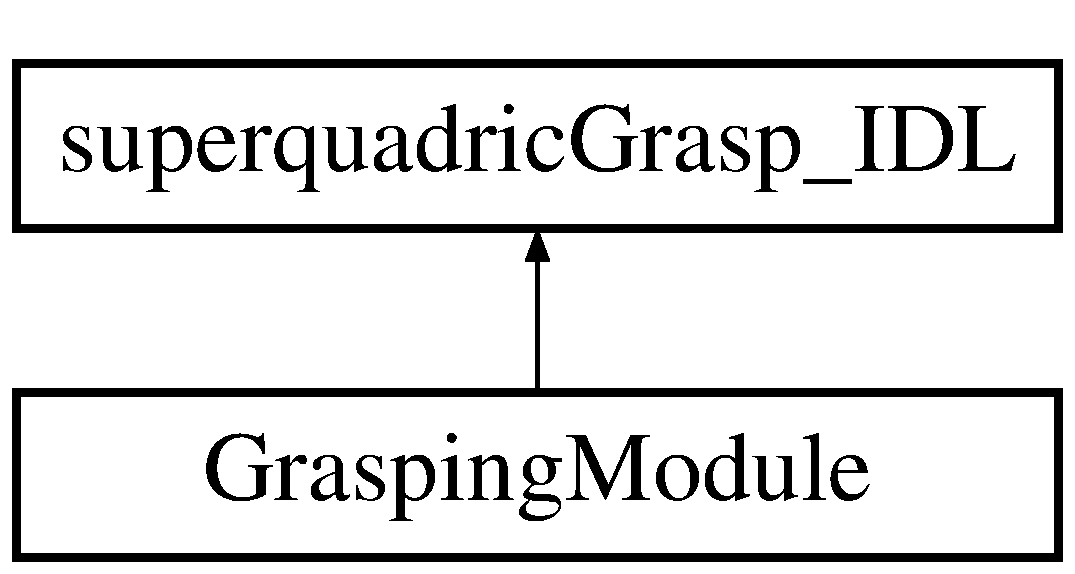
\includegraphics[height=2.000000cm]{classGraspingModule}
\end{center}
\end{figure}
\subsection*{Public Member Functions}
\begin{DoxyCompactItemize}
\item 
bool {\bfseries attach} (yarp\+::os\+::\+Rpc\+Server \&source)\label{classGraspingModule_ac3e7a265105f99952742a6aca17d67c3}

\item 
std\+::string \hyperlink{classGraspingModule_aabedec650875263d27ecf20fa9dd8b39}{get\+\_\+visualization} ()
\begin{DoxyCompactList}\small\item\em Return if visualization is on or off. \end{DoxyCompactList}\item 
bool \hyperlink{classGraspingModule_a801de4b63aba360a4b85e322c5947a4a}{set\+\_\+visualization} (const std\+::string \&e)
\begin{DoxyCompactList}\small\item\em Set visualization option on or off. \end{DoxyCompactList}\item 
std\+::string \hyperlink{classGraspingModule_a5103f8bd6671a11a9bd1c7e29d290009}{get\+\_\+best\+\_\+hand} ()
\begin{DoxyCompactList}\small\item\em Return the computed grasping poses. \end{DoxyCompactList}\item 
yarp\+::os\+::\+Property \hyperlink{classGraspingModule_af1e057f767ab83be185cf486d3f5c46b}{get\+\_\+grasping\+\_\+pose} (const yarp\+::os\+::\+Property \&superquadric, const std\+::string \&hand)
\begin{DoxyCompactList}\small\item\em Return the estimated grasping poses given an estimated superquadric. \end{DoxyCompactList}\item 
yarp\+::os\+::\+Property \hyperlink{classGraspingModule_a375475691c644d8aa882db8d65ceda50}{get\+\_\+options} (const std\+::string \&field)
\begin{DoxyCompactList}\small\item\em Get options of the field of interest. \end{DoxyCompactList}\item 
bool \hyperlink{classGraspingModule_a849c459ef9700c93b45ef6cff394f675}{set\+\_\+options} (const yarp\+::os\+::\+Property \&new\+Options, const std\+::string \&field)
\begin{DoxyCompactList}\small\item\em Set options of the field of interest. \end{DoxyCompactList}\item 
std\+::string \hyperlink{classGraspingModule_a557a87131c7396dd62c02eced7f4a937}{get\+\_\+hand} ()
\begin{DoxyCompactList}\small\item\em Return which hand has been enabled. \end{DoxyCompactList}\item 
bool \hyperlink{classGraspingModule_a9d34cb0521f86dd16648255e640eec90}{set\+\_\+hand} (const std\+::string \&e)
\begin{DoxyCompactList}\small\item\em Set hand enabled. \end{DoxyCompactList}\item 
bool \hyperlink{classGraspingModule_a618785dec349358760a05e6e4b097866}{set\+\_\+save\+\_\+poses} (const std\+::string \&entry)
\begin{DoxyCompactList}\small\item\em Return if poses are saved or not. \end{DoxyCompactList}\item 
std\+::string \hyperlink{classGraspingModule_a949e4297bdf26f564669ffc91068c4f3}{get\+\_\+save\+\_\+poses} ()
\begin{DoxyCompactList}\small\item\em Set if poses are saved or not. \end{DoxyCompactList}\item 
yarp\+::os\+::\+Property \hyperlink{classGraspingModule_a059da011f804acd1adc4549eaa3d2141}{fill\+Property} (const yarp\+::sig\+::\+Vector \&sol)
\begin{DoxyCompactList}\small\item\em Fill property with the grasping solutions. \end{DoxyCompactList}\item 
bool \hyperlink{classGraspingModule_a834e972a2a1b7b92bf8dc1e83319b028}{clear\+\_\+poses} ()
\begin{DoxyCompactList}\small\item\em Delete computed poses. \end{DoxyCompactList}\item 
bool \hyperlink{classGraspingModule_a08bd9cdbb1d16da8616c9769510e2bf1}{move} (const std\+::string \&entry)
\begin{DoxyCompactList}\small\item\em Move the selected arm. \end{DoxyCompactList}\item 
bool \hyperlink{classGraspingModule_a518ee4ec1b27d32c600f340c0f3bf552}{config\+Basics} (yarp\+::os\+::\+Resource\+Finder \&rf)
\begin{DoxyCompactList}\small\item\em Configure basics options. \end{DoxyCompactList}\item 
bool \hyperlink{classGraspingModule_a151b46117f2d1fdd8c321554012d63f3}{close} ()
\begin{DoxyCompactList}\small\item\em Close function of the RF module. \end{DoxyCompactList}\item 
bool \hyperlink{classGraspingModule_aca7dc9ec5e0a98b1333ed4c63650cdba}{interrupt\+Module} ()
\begin{DoxyCompactList}\small\item\em Interrupt function of the RF module. \end{DoxyCompactList}\item 
bool \hyperlink{classGraspingModule_af2cd7fa157b5d78080ffd7952655046d}{update\+Module} ()
\begin{DoxyCompactList}\small\item\em Update function of the RF module. \end{DoxyCompactList}\item 
double \hyperlink{classGraspingModule_abfc60b8437d750f2b2a48b8a617e53c1}{get\+Period} ()
\begin{DoxyCompactList}\small\item\em Get period function of the RF module. \end{DoxyCompactList}\item 
bool \hyperlink{classGraspingModule_a1086203a4db1e465ef8aba5e28f60025}{config\+Viewer} (yarp\+::os\+::\+Resource\+Finder \&rf)
\begin{DoxyCompactList}\small\item\em Configure options for visualization. \end{DoxyCompactList}\item 
bool \hyperlink{classGraspingModule_ab6d6d4c684340a0e4988a338ff72e3d0}{config\+Pose} (yarp\+::os\+::\+Resource\+Finder \&rf)
\begin{DoxyCompactList}\small\item\em Configure options for pose computation. \end{DoxyCompactList}\item 
bool \hyperlink{classGraspingModule_af83c4dc5cdc8ed18a03ce2637abda2e9}{config\+Movements} (yarp\+::os\+::\+Resource\+Finder \&rf)
\begin{DoxyCompactList}\small\item\em Configure options for arm movements. \end{DoxyCompactList}\item 
bool \hyperlink{classGraspingModule_a31c82e1ba3c80d1238e95449780f62c6}{config\+Grasp} (yarp\+::os\+::\+Resource\+Finder \&rf)
\begin{DoxyCompactList}\small\item\em Configure options for grasping. \end{DoxyCompactList}\item 
bool \hyperlink{classGraspingModule_ab4c0ea3cabb2cc6de63da53ba1771e27}{configure} (yarp\+::os\+::\+Resource\+Finder \&rf)\label{classGraspingModule_ab4c0ea3cabb2cc6de63da53ba1771e27}

\begin{DoxyCompactList}\small\item\em Configure function of RF module. \end{DoxyCompactList}\item 
bool \hyperlink{classGraspingModule_aa1c32186a8b7133db63e115898949b28}{read\+Superq} (const std\+::string \&name\+\_\+obj, yarp\+::sig\+::\+Vector \&x, const int \&dimension, yarp\+::os\+::\+Resource\+Finder $\ast$rf)
\begin{DoxyCompactList}\small\item\em Read object model from text file for simulation tests. \end{DoxyCompactList}\item 
void \hyperlink{classGraspingModule_a43a89c97919dd68a4ab28a6c9fe16a95}{save\+Sol} (const yarp\+::os\+::\+Property \&sol)
\begin{DoxyCompactList}\small\item\em Save solutions. \end{DoxyCompactList}\item 
bool {\bfseries look\+\_\+center} ()\label{classGraspingModule_af640219e03fdfe6e6145a5ff6f01d23a}

\item 
bool {\bfseries look\+\_\+obj} ()\label{classGraspingModule_a741cac4968db05d8dde9cd1856776c50}

\item 
bool \hyperlink{classGraspingModule_a1455fc4c6a1ae5690fa691cc324fec4e}{go\+\_\+home} (const std\+::string \&entry)
\begin{DoxyCompactList}\small\item\em Go back to home position. \end{DoxyCompactList}\item 
bool \hyperlink{classGraspingModule_a75482819f7f289b3f456571628952122}{go\+\_\+to\+\_\+basket} (const std\+::string \&entry)
\begin{DoxyCompactList}\small\item\em Go back to the basket on the robot side. \end{DoxyCompactList}\item 
bool \hyperlink{classGraspingModule_a91eac72e632f224442f34b907e479fa3}{check\+\_\+motion} ()
\begin{DoxyCompactList}\small\item\em Check if the motion has been completed. \end{DoxyCompactList}\item 
bool \hyperlink{classGraspingModule_a650c026153e3a7b0044f508cf9d4bf00}{check\+\_\+home} ()
\begin{DoxyCompactList}\small\item\em Check if the motion back to home has been completed. \end{DoxyCompactList}\item 
bool \hyperlink{classGraspingModule_a19ee1967a83d1412f9125ec482ce80bd}{check\+\_\+basket} ()
\begin{DoxyCompactList}\small\item\em Check if the motion to the basket has been completed. \end{DoxyCompactList}\item 
virtual bool \hyperlink{classsuperquadricGrasp__IDL_ac40ef7c0dd4f0e3600db9aea5cc5c298}{calibrate} ()
\begin{DoxyCompactList}\small\item\em Calibrate plane height via superquadric computation. \end{DoxyCompactList}\item 
virtual bool {\bfseries read} (yarp\+::os\+::\+Connection\+Reader \&connection) Y\+A\+R\+P\+\_\+\+O\+V\+E\+R\+R\+I\+DE\label{classsuperquadricGrasp__IDL_a710271cfee0c9b1a31707d84f194b69b}

\item 
virtual std\+::vector$<$ std\+::string $>$ {\bfseries help} (const std\+::string \&function\+Name=\char`\"{}-\/-\/all\char`\"{})\label{classsuperquadricGrasp__IDL_a226f766d3a3a0ba87e7c1fa0aceb2cb8}

\end{DoxyCompactItemize}
\subsection*{Protected Attributes}
\begin{DoxyCompactItemize}
\item 
yarp\+::os\+::\+Resource\+Finder $\ast$ {\bfseries rf}\label{classGraspingModule_aed592146c8031a537a8d1f71a7e054c5}

\item 
std\+::string {\bfseries robot}\label{classGraspingModule_a508cc33e7003b294f00316f362f82eaa}

\item 
std\+::string {\bfseries left\+\_\+or\+\_\+right}\label{classGraspingModule_ab9603885e438ebe5a7f673c04bc37ed8}

\item 
std\+::string {\bfseries home\+Context\+Path}\label{classGraspingModule_a0aa116f84336b88479b6f3ac6a97e76b}

\item 
yarp\+::sig\+::\+Vector {\bfseries poseL}\label{classGraspingModule_ae819bea3ec49cbec2703737a7a786007}

\item 
yarp\+::sig\+::\+Vector {\bfseries solL}\label{classGraspingModule_a0a13dee5ac1b2db61a87f82ecdc44ea6}

\item 
yarp\+::sig\+::\+Vector {\bfseries poseR}\label{classGraspingModule_a148c46809e3dba05972df158c81c48f8}

\item 
yarp\+::sig\+::\+Vector {\bfseries solR}\label{classGraspingModule_a1215352771f0e7f26e033ad95731a81e}

\item 
std\+::deque$<$ yarp\+::sig\+::\+Vector $>$ {\bfseries trajectory\+\_\+right}\label{classGraspingModule_ac7c1f1dc2e81ed15f87218feaa038988}

\item 
std\+::deque$<$ yarp\+::sig\+::\+Vector $>$ {\bfseries trajectory\+\_\+left}\label{classGraspingModule_afcfe41fdc6ce4446e89594a3d40d2a7d}

\item 
int {\bfseries context\+\_\+gaze}\label{classGraspingModule_ab87532f4790da036cdf51654a649cece}

\item 
int {\bfseries rate\+\_\+vis}\label{classGraspingModule_a26e3aee1196f9b3783426f5be6a387b5}

\item 
int {\bfseries print\+\_\+level}\label{classGraspingModule_a244cb8f6f2b2294d2be164ee1518cc36}

\item 
double {\bfseries t}\label{classGraspingModule_a4f36c3ca4e343f62ec908768af45a3da}

\item 
double {\bfseries t0}\label{classGraspingModule_a70a4e9c60616c7e7c63b11594e73a6ac}

\item 
double {\bfseries t\+\_\+grasp}\label{classGraspingModule_aaf674331d6bbf84ea008566948c6dee2}

\item 
double {\bfseries t\+\_\+vis}\label{classGraspingModule_ae0cddf0f4c4e7d00197a1c45ff98f0e5}

\item 
std\+::deque$<$ double $>$ {\bfseries times\+\_\+vis}\label{classGraspingModule_a9a0dedfb6b400af32cd04a9eafd43dba}

\item 
double {\bfseries tol}\label{classGraspingModule_a521b7c66535fb4dac516a9ff58241f05}

\item 
int {\bfseries max\+\_\+iter}\label{classGraspingModule_a3f17b0601f067499b5f574fb8c6f937e}

\item 
int {\bfseries n\+\_\+pointshand}\label{classGraspingModule_aa4dff98eeb8125bc88613b15159cd26c}

\item 
int {\bfseries acceptable\+\_\+iter}\label{classGraspingModule_ab3821aa16b5021be595ac8b7db4d6cfb}

\item 
double {\bfseries constr\+\_\+viol\+\_\+tol}\label{classGraspingModule_a5529bf668b7ea95582ea238d5f50e3c2}

\item 
std\+::string {\bfseries mu\+\_\+strategy}\label{classGraspingModule_a64763408867f3cb6dc508c91f8cf220a}

\item 
std\+::string {\bfseries nlp\+\_\+scaling\+\_\+method}\label{classGraspingModule_aecc5738f9012849c9edaf35f479723b4}

\item 
double {\bfseries max\+\_\+cpu\+\_\+time}\label{classGraspingModule_a3dabf2eac967efb30b1b7bb9c91e41b3}

\item 
std\+::string {\bfseries dir}\label{classGraspingModule_a87c885eada6df4d622c92173d8a4ed2e}

\item 
yarp\+::sig\+::\+Vector {\bfseries object}\label{classGraspingModule_a4b3ada8a9325ed821e73b8e84375c4fa}

\item 
yarp\+::sig\+::\+Vector {\bfseries hand}\label{classGraspingModule_af8308a8938957b4bb50c260dc42d7b27}

\item 
yarp\+::sig\+::\+Vector {\bfseries hand1}\label{classGraspingModule_a0b4986d666ef55b1c769d1b02b49c86f}

\item 
double {\bfseries distance}\label{classGraspingModule_af1912ddc2800fb3101e98a99d3b04b5b}

\item 
double {\bfseries distance1}\label{classGraspingModule_aacb0581ba76204e825aee632cf9679e4}

\item 
yarp\+::sig\+::\+Vector {\bfseries displacement}\label{classGraspingModule_a52131b73f3688ab8524f37b8e1945717}

\item 
yarp\+::sig\+::\+Vector {\bfseries plane}\label{classGraspingModule_a234e3ab635ba9b581e6877519dc633b6}

\item 
yarp\+::os\+::\+Rpc\+Server {\bfseries port\+Rpc}\label{classGraspingModule_a164dc4c91253669941ad45e2702bb746}

\item 
std\+::string {\bfseries eye}\label{classGraspingModule_a2d764f516aecffb52ba22f1dcdd2a730}

\item 
double {\bfseries block\+\_\+eye}\label{classGraspingModule_a9562cc675af9a861201956fe23a267bc}

\item 
double {\bfseries block\+\_\+neck}\label{classGraspingModule_aa92c21ad6a4a5f70f73ebf3281676f62}

\item 
yarp\+::sig\+::\+Matrix {\bfseries K}\label{classGraspingModule_a161a8c4d8bc2db6e1cf7c00a69953831}

\item 
yarp\+::sig\+::\+Matrix {\bfseries H}\label{classGraspingModule_acb55c5d37d9a7225b44323d2be724bfe}

\item 
yarp\+::dev\+::\+Poly\+Driver {\bfseries Gaze\+Ctrl}\label{classGraspingModule_adfed9afcb5290a5ee2e99768352fd4fb}

\item 
yarp\+::dev\+::\+I\+Gaze\+Control $\ast$ {\bfseries igaze}\label{classGraspingModule_a70a410aead666d7198eb183ba05472a5}

\item 
std\+::string {\bfseries fing}\label{classGraspingModule_ad33afeaa6a6b67f3f49ccb4ee771e6cb}

\item 
bool {\bfseries lift\+\_\+object}\label{classGraspingModule_ae7f23202919c7dbd742230a2cc005043}

\item 
std\+::string {\bfseries lobj}\label{classGraspingModule_af871b2ab1e5110408893eef5ac711984}

\item 
bool {\bfseries go\+\_\+on}\label{classGraspingModule_aa1da1c0d76de383f74360bc9c9125e77}

\item 
bool {\bfseries grasp}\label{classGraspingModule_ae56f0d9a9eed5d68051da744dac15a41}

\item 
bool {\bfseries executed}\label{classGraspingModule_a499af38a89686312a34117c0218fc6cb}

\item 
bool {\bfseries executed\+\_\+var}\label{classGraspingModule_abdcf071d6ce460a83c56ef1ba90f8b1f}

\item 
bool {\bfseries reached\+\_\+home}\label{classGraspingModule_af46e9f6a4a79bb39db0f975803d739b3}

\item 
bool {\bfseries reached\+\_\+basket}\label{classGraspingModule_a295ffc6e5c40dea6d6e222f3f487ec67}

\item 
std\+::string {\bfseries show\+\_\+hand}\label{classGraspingModule_af05d3fc99e87d5ab513bb9fe91f0bcea}

\item 
std\+::string {\bfseries show\+\_\+only\+\_\+pose}\label{classGraspingModule_ae9a9a1e59ba2298fac3c4f34996ec25e}

\item 
std\+::string {\bfseries look\+\_\+object}\label{classGraspingModule_ac74a028982f21c24a3405deb41e70f9f}

\item 
bool {\bfseries visualization}\label{classGraspingModule_afb42ea3b2951d1e8abe7f391675d8f73}

\item 
bool {\bfseries mode\+\_\+online}\label{classGraspingModule_afa54033aed276e29223d9a88a6f7f145}

\item 
bool {\bfseries save\+\_\+poses}\label{classGraspingModule_a8193f9e7fc2e65f52bf80580735113bc}

\item 
bool {\bfseries also\+\_\+traj}\label{classGraspingModule_ada586ca7d90ea75cf6be9847ddb274c7}

\item 
double {\bfseries force\+\_\+threshold}\label{classGraspingModule_abd2e8eaca9dd18e74a40fd3831922c16}

\item 
std\+::string {\bfseries compliant}\label{classGraspingModule_ad74775f47ff255bde51b0bab79a31728}

\item 
std\+::string {\bfseries visual\+\_\+servoing}\label{classGraspingModule_a79082a891f887dbb9edfed4653451e35}

\item 
std\+::string {\bfseries use\+\_\+direct\+\_\+kin}\label{classGraspingModule_a832c738961170cb80a024805b22464b8}

\item 
double {\bfseries pixel\+\_\+tol}\label{classGraspingModule_aa84058eee1411f35aa489b9cad9f9371}

\item 
double {\bfseries lift\+\_\+z}\label{classGraspingModule_a676c7aa895de03ba5362a309cd669905}

\item 
double {\bfseries torso\+\_\+pitch\+\_\+max}\label{classGraspingModule_af1feeb0f4397d83491831327e05c8b44}

\item 
double {\bfseries traj\+\_\+time}\label{classGraspingModule_a02accb5392fe0877a2a98febbcf20ea6}

\item 
double {\bfseries traj\+\_\+tol}\label{classGraspingModule_a2b59e1c09ae51bb1829cb4b73799a9d2}

\item 
yarp\+::sig\+::\+Vector {\bfseries shift\+\_\+right}\label{classGraspingModule_a589b2e394e0d255fcd23734b911392ef}

\item 
yarp\+::sig\+::\+Vector {\bfseries shift\+\_\+left}\label{classGraspingModule_a96feca3ff9d44e599351ddb1c4497fcf}

\item 
yarp\+::sig\+::\+Vector {\bfseries home\+\_\+right}\label{classGraspingModule_ac43f827abab558d8aea39a6cbcd150a2}

\item 
yarp\+::sig\+::\+Vector {\bfseries home\+\_\+left}\label{classGraspingModule_a75a4689473261072a85c67c76ac6567f}

\item 
yarp\+::sig\+::\+Vector {\bfseries basket\+\_\+right}\label{classGraspingModule_a514ee9d4045d3e551a089ffd1f296c49}

\item 
yarp\+::sig\+::\+Vector {\bfseries basket\+\_\+left}\label{classGraspingModule_a4c2cf37b608df9bdce4ff5a2882111ef}

\item 
yarp\+::sig\+::\+Vector {\bfseries stiff\+\_\+right}\label{classGraspingModule_af25aefd74e3a455cd3288896dc7f545e}

\item 
yarp\+::sig\+::\+Vector {\bfseries stiff\+\_\+left}\label{classGraspingModule_a39f2ad508bb3f5baeac30684cd57bf44}

\item 
yarp\+::sig\+::\+Vector {\bfseries damp\+\_\+right}\label{classGraspingModule_af7690eeb0850a02dc05e20e4c4326dd4}

\item 
yarp\+::sig\+::\+Vector {\bfseries damp\+\_\+left}\label{classGraspingModule_ad4dda6219b8a0bf9636c7bf58effc14b}

\item 
std\+::string {\bfseries hand\+\_\+to\+\_\+move}\label{classGraspingModule_af119be2a7acbb0568d1c08f4f6069928}

\item 
std\+::string {\bfseries name\+File\+Out\+\_\+right}\label{classGraspingModule_a627ae74edcebd1e63427d1923bf07004}

\item 
std\+::string {\bfseries name\+File\+Trajectory\+\_\+right}\label{classGraspingModule_a2d67456b32002aeca338be1844e5fe79}

\item 
std\+::string {\bfseries name\+File\+Out\+\_\+left}\label{classGraspingModule_a3d16b71a4e021206b2b60dca65b6bf88}

\item 
std\+::string {\bfseries name\+File\+Trajectory\+\_\+left}\label{classGraspingModule_a1f3841076509b5140edbdb7d01aa3f4b}

\item 
std\+::string {\bfseries lib\+\_\+context}\label{classGraspingModule_a7d96e2271d553a340888ffa1a422d608}

\item 
std\+::string {\bfseries lib\+\_\+filename}\label{classGraspingModule_a437d621f1b6e1ce0d5cc1d8958b53fee}

\item 
yarp\+::os\+::\+Mutex {\bfseries mutex}\label{classGraspingModule_ae27bf275f6a5f99728586ae235477683}

\item 
\hyperlink{classGraspComputation}{Grasp\+Computation} $\ast$ {\bfseries grasp\+Comp}\label{classGraspingModule_a2a88d576e1cc46c209d6ff40657f1ddb}

\item 
\hyperlink{classGraspVisualization}{Grasp\+Visualization} $\ast$ {\bfseries grasp\+Vis}\label{classGraspingModule_a98acb57493a68c3ce14f6e89b721aa23}

\item 
\hyperlink{classGraspExecution}{Grasp\+Execution} $\ast$ {\bfseries grasp\+Exec}\label{classGraspingModule_a1c5e0b94e7b086d14ac1bf45db3007f1}

\item 
yarp\+::os\+::\+Property {\bfseries vis\+\_\+par}\label{classGraspingModule_a2d8f2bb7d5263b2df89d7431fe830525}

\item 
yarp\+::os\+::\+Property {\bfseries pose\+\_\+par}\label{classGraspingModule_ac5132578e072a0cd851a888487d4e144}

\item 
yarp\+::os\+::\+Property {\bfseries traj\+\_\+par}\label{classGraspingModule_a4fde085a2948717e65736a75a2786a0d}

\item 
yarp\+::os\+::\+Property {\bfseries grasp\+\_\+par}\label{classGraspingModule_a8665afdacf9d155c465fb7497d202fba}

\item 
yarp\+::os\+::\+Property {\bfseries ipopt\+\_\+par}\label{classGraspingModule_af17896b5afa9de9dbd63caf2bf4e2deb}

\item 
yarp\+::os\+::\+Property {\bfseries movement\+\_\+par}\label{classGraspingModule_a7da5cb35f5a34a18b68023c3d1d3f276}

\item 
yarp\+::os\+::\+Property {\bfseries complete\+\_\+sol}\label{classGraspingModule_af0bdebfd4648ff04bcaf790879897743}

\item 
double {\bfseries quality\+\_\+right}\label{classGraspingModule_aca01f7f0ec39c36623700330b632109f}

\item 
double {\bfseries quality\+\_\+left}\label{classGraspingModule_a6f5ca6d1a1e4efceb05d32fb9c0e10ad}

\end{DoxyCompactItemize}


\subsection{Detailed Description}
This class handles the grasping pose computation and visualization, together with the interaction with the user. 

In particular, it launches the visualization thread and implements a state machine for handling the grasping pose computation and excution. 

Definition at line 39 of file grasp\+Module.\+h.



\subsection{Member Function Documentation}
\index{Grasping\+Module@{Grasping\+Module}!calibrate@{calibrate}}
\index{calibrate@{calibrate}!Grasping\+Module@{Grasping\+Module}}
\subsubsection[{\texorpdfstring{calibrate()}{calibrate()}}]{\setlength{\rightskip}{0pt plus 5cm}virtual bool superquadric\+Grasp\+\_\+\+I\+D\+L\+::calibrate (
\begin{DoxyParamCaption}
{}
\end{DoxyParamCaption}
)\hspace{0.3cm}{\ttfamily [virtual]}, {\ttfamily [inherited]}}\label{classsuperquadricGrasp__IDL_ac40ef7c0dd4f0e3600db9aea5cc5c298}


Calibrate plane height via superquadric computation. 

\begin{DoxyReturn}{Returns}
true/false on success/failure. 
\end{DoxyReturn}
\index{Grasping\+Module@{Grasping\+Module}!check\+\_\+basket@{check\+\_\+basket}}
\index{check\+\_\+basket@{check\+\_\+basket}!Grasping\+Module@{Grasping\+Module}}
\subsubsection[{\texorpdfstring{check\+\_\+basket()}{check_basket()}}]{\setlength{\rightskip}{0pt plus 5cm}bool Grasping\+Module\+::check\+\_\+basket (
\begin{DoxyParamCaption}
{}
\end{DoxyParamCaption}
)}\label{classGraspingModule_a19ee1967a83d1412f9125ec482ce80bd}


Check if the motion to the basket has been completed. 

\begin{DoxyReturn}{Returns}
true/false on success/failure 
\end{DoxyReturn}


Definition at line 289 of file grasp\+Module.\+cpp.


\begin{DoxyCode}
290 \{
291     \textcolor{keywordflow}{return} reached\_basket;
292 \}
\end{DoxyCode}
\index{Grasping\+Module@{Grasping\+Module}!check\+\_\+home@{check\+\_\+home}}
\index{check\+\_\+home@{check\+\_\+home}!Grasping\+Module@{Grasping\+Module}}
\subsubsection[{\texorpdfstring{check\+\_\+home()}{check_home()}}]{\setlength{\rightskip}{0pt plus 5cm}bool Grasping\+Module\+::check\+\_\+home (
\begin{DoxyParamCaption}
{}
\end{DoxyParamCaption}
)\hspace{0.3cm}{\ttfamily [virtual]}}\label{classGraspingModule_a650c026153e3a7b0044f508cf9d4bf00}


Check if the motion back to home has been completed. 

\begin{DoxyReturn}{Returns}
true/false on success/failure 
\end{DoxyReturn}


Reimplemented from \hyperlink{classsuperquadricGrasp__IDL_a9e11fd04a40c86987500c42f898508ea}{superquadric\+Grasp\+\_\+\+I\+DL}.



Definition at line 283 of file grasp\+Module.\+cpp.


\begin{DoxyCode}
284 \{
285     \textcolor{keywordflow}{return} reached\_home;
286 \}
\end{DoxyCode}
\index{Grasping\+Module@{Grasping\+Module}!check\+\_\+motion@{check\+\_\+motion}}
\index{check\+\_\+motion@{check\+\_\+motion}!Grasping\+Module@{Grasping\+Module}}
\subsubsection[{\texorpdfstring{check\+\_\+motion()}{check_motion()}}]{\setlength{\rightskip}{0pt plus 5cm}bool Grasping\+Module\+::check\+\_\+motion (
\begin{DoxyParamCaption}
{}
\end{DoxyParamCaption}
)\hspace{0.3cm}{\ttfamily [virtual]}}\label{classGraspingModule_a91eac72e632f224442f34b907e479fa3}


Check if the motion has been completed. 

\begin{DoxyReturn}{Returns}
true/false on success/failure 
\end{DoxyReturn}


Reimplemented from \hyperlink{classsuperquadricGrasp__IDL_afd0cc265ba84c844aee5654f1a713fbd}{superquadric\+Grasp\+\_\+\+I\+DL}.



Definition at line 277 of file grasp\+Module.\+cpp.


\begin{DoxyCode}
278 \{
279     \textcolor{keywordflow}{return} executed\_var;
280 \}
\end{DoxyCode}
\index{Grasping\+Module@{Grasping\+Module}!clear\+\_\+poses@{clear\+\_\+poses}}
\index{clear\+\_\+poses@{clear\+\_\+poses}!Grasping\+Module@{Grasping\+Module}}
\subsubsection[{\texorpdfstring{clear\+\_\+poses()}{clear_poses()}}]{\setlength{\rightskip}{0pt plus 5cm}bool Grasping\+Module\+::clear\+\_\+poses (
\begin{DoxyParamCaption}
{}
\end{DoxyParamCaption}
)\hspace{0.3cm}{\ttfamily [virtual]}}\label{classGraspingModule_a834e972a2a1b7b92bf8dc1e83319b028}


Delete computed poses. 

\begin{DoxyReturn}{Returns}
true/false 
\end{DoxyReturn}


Reimplemented from \hyperlink{classsuperquadricGrasp__IDL_a6d1e4533ad8b34510ba9792f7cd72113}{superquadric\+Grasp\+\_\+\+I\+DL}.



Definition at line 46 of file grasp\+Module.\+cpp.


\begin{DoxyCode}
47 \{
48     LockGuard lg(mutex);
49 
50     poseR.resize(6,0.0);
51     poseL.resize(6,0.0);
52     \textcolor{keywordtype}{object}.resize(11,0.0);
53     complete\_sol.clear();
54 
55     \textcolor{keywordflow}{return} \textcolor{keyword}{true};
56 \}
\end{DoxyCode}
\index{Grasping\+Module@{Grasping\+Module}!close@{close}}
\index{close@{close}!Grasping\+Module@{Grasping\+Module}}
\subsubsection[{\texorpdfstring{close()}{close()}}]{\setlength{\rightskip}{0pt plus 5cm}bool Grasping\+Module\+::close (
\begin{DoxyParamCaption}
{}
\end{DoxyParamCaption}
)}\label{classGraspingModule_a151b46117f2d1fdd8c321554012d63f3}


Close function of the RF module. 

\begin{DoxyReturn}{Returns}
true/false on success/failure 
\end{DoxyReturn}


Definition at line 545 of file grasp\+Module.\+cpp.


\begin{DoxyCode}
546 \{
547     \textcolor{keyword}{delete} graspComp;
548 
549     graspExec->release();
550     \textcolor{keyword}{delete} graspExec;
551 
552     \textcolor{keywordflow}{if} (visualization)
553         graspVis->stop();
554 
555     \textcolor{keyword}{delete} graspVis;
556 
557     \textcolor{keywordflow}{if} (portRpc.asPort().isOpen())
558         portRpc.close();
559 
560     igaze->stopControl();
561 
562     igaze->restoreContext(context\_gaze);
563 
564     GazeCtrl.close();
565 
566     \textcolor{keywordflow}{return} \textcolor{keyword}{true};
567 \}
\end{DoxyCode}
\index{Grasping\+Module@{Grasping\+Module}!config\+Basics@{config\+Basics}}
\index{config\+Basics@{config\+Basics}!Grasping\+Module@{Grasping\+Module}}
\subsubsection[{\texorpdfstring{config\+Basics(yarp\+::os\+::\+Resource\+Finder \&rf)}{configBasics(yarp::os::ResourceFinder &rf)}}]{\setlength{\rightskip}{0pt plus 5cm}bool Grasping\+Module\+::config\+Basics (
\begin{DoxyParamCaption}
\item[{yarp\+::os\+::\+Resource\+Finder \&}]{rf}
\end{DoxyParamCaption}
)}\label{classGraspingModule_a518ee4ec1b27d32c600f340c0f3bf552}


Configure basics options. 


\begin{DoxyParams}{Parameters}
{\em rf} & is the resource finder with all the options from config files \\
\hline
\end{DoxyParams}
\begin{DoxyReturn}{Returns}
true/false on success/failure 
\end{DoxyReturn}


Definition at line 377 of file grasp\+Module.\+cpp.


\begin{DoxyCode}
378 \{
379     homeContextPath=rf.getHomeContextPath().c\_str();
380 
381     robot=rf.find(\textcolor{stringliteral}{"robot"}).asString().c\_str();
382     \textcolor{keywordflow}{if}(rf.find(\textcolor{stringliteral}{"robot"}).isNull())
383         robot=\textcolor{stringliteral}{"icubSim"};
384 
385     left\_or\_right=rf.find(\textcolor{stringliteral}{"which\_hand"}).asString().c\_str();
386 
387     \textcolor{keywordflow}{if}(rf.find(\textcolor{stringliteral}{"which\_hand"}).isNull())
388         left\_or\_right=\textcolor{stringliteral}{"right"};
389 
390     portRpc.open(\textcolor{stringliteral}{"/superquadric-grasp/rpc"});
391     attach(portRpc);
392 
393     dir=rf.check(\textcolor{stringliteral}{"approaching\_direction"}, Value(\textcolor{stringliteral}{"z"})).asString();
394     rate\_vis=rf.check(\textcolor{stringliteral}{"rate\_vis"}, Value(100)).asInt();
395     mode\_online=(rf.check(\textcolor{stringliteral}{"mode\_online"}, Value(\textcolor{stringliteral}{"on"})).asString()==\textcolor{stringliteral}{"on"});
396     save\_poses=(rf.check(\textcolor{stringliteral}{"save\_poses"}, Value(\textcolor{stringliteral}{"on"})).asString()==\textcolor{stringliteral}{"on"});
397     also\_traj=(rf.check(\textcolor{stringliteral}{"also\_traj"}, Value(\textcolor{stringliteral}{"off"})).asString()==\textcolor{stringliteral}{"on"});
398     visualization=(rf.check(\textcolor{stringliteral}{"visualization"}, Value(\textcolor{stringliteral}{"off"})).asString()==\textcolor{stringliteral}{"on"});
399     grasp=(rf.check(\textcolor{stringliteral}{"grasp"}, Value(\textcolor{stringliteral}{"off"})).asString()==\textcolor{stringliteral}{"on"});
400     visual\_servoing=rf.check(\textcolor{stringliteral}{"visual\_servoing"}, Value(\textcolor{stringliteral}{"off"})).asString();   
401     compliant=rf.check(\textcolor{stringliteral}{"compliant"}, Value(\textcolor{stringliteral}{"off"})).asString();
402     use\_direct\_kin=rf.check(\textcolor{stringliteral}{"use\_direct\_kin"}, Value(\textcolor{stringliteral}{"off"})).asString();
403     print\_level=rf.check(\textcolor{stringliteral}{"print\_level"}, Value(0)).asInt();
404 
405     go\_on=\textcolor{keyword}{false};
406 
407     \textcolor{keywordflow}{return} \textcolor{keyword}{true};
408 \}
\end{DoxyCode}
\index{Grasping\+Module@{Grasping\+Module}!config\+Grasp@{config\+Grasp}}
\index{config\+Grasp@{config\+Grasp}!Grasping\+Module@{Grasping\+Module}}
\subsubsection[{\texorpdfstring{config\+Grasp(yarp\+::os\+::\+Resource\+Finder \&rf)}{configGrasp(yarp::os::ResourceFinder &rf)}}]{\setlength{\rightskip}{0pt plus 5cm}bool Grasping\+Module\+::config\+Grasp (
\begin{DoxyParamCaption}
\item[{yarp\+::os\+::\+Resource\+Finder \&}]{rf}
\end{DoxyParamCaption}
)}\label{classGraspingModule_a31c82e1ba3c80d1238e95449780f62c6}


Configure options for grasping. 


\begin{DoxyParams}{Parameters}
{\em rf} & is the resource finder with all the optins \\
\hline
\end{DoxyParams}
\begin{DoxyReturn}{Returns}
true/false on success/failure 
\end{DoxyReturn}


Definition at line 536 of file grasp\+Module.\+cpp.


\begin{DoxyCode}
537 \{
538     lib\_context=rf.check(\textcolor{stringliteral}{"lib\_context"}, Value(\textcolor{stringliteral}{"superquadric-grasp"})).asString();
539     lib\_filename=rf.check(\textcolor{stringliteral}{"lib\_filename"}, Value(\textcolor{stringliteral}{"confTactileControlLib"})).asString();
540 
541     \textcolor{keywordflow}{return} \textcolor{keyword}{true};
542 \}
\end{DoxyCode}
\index{Grasping\+Module@{Grasping\+Module}!config\+Movements@{config\+Movements}}
\index{config\+Movements@{config\+Movements}!Grasping\+Module@{Grasping\+Module}}
\subsubsection[{\texorpdfstring{config\+Movements(yarp\+::os\+::\+Resource\+Finder \&rf)}{configMovements(yarp::os::ResourceFinder &rf)}}]{\setlength{\rightskip}{0pt plus 5cm}bool Grasping\+Module\+::config\+Movements (
\begin{DoxyParamCaption}
\item[{yarp\+::os\+::\+Resource\+Finder \&}]{rf}
\end{DoxyParamCaption}
)}\label{classGraspingModule_af83c4dc5cdc8ed18a03ce2637abda2e9}


Configure options for arm movements. 


\begin{DoxyParams}{Parameters}
{\em rf} & is the resource finder with all the optins \\
\hline
\end{DoxyParams}
\begin{DoxyReturn}{Returns}
true/false on success/failure 
\end{DoxyReturn}


Definition at line 411 of file grasp\+Module.\+cpp.


\begin{DoxyCode}
412 \{
413     traj\_time=rf.check(\textcolor{stringliteral}{"trajectory\_time"}, Value(1.0)).asDouble();
414     traj\_tol=rf.check(\textcolor{stringliteral}{"trajectory\_tol"}, Value(0.01)).asDouble();
415     pixel\_tol=rf.check(\textcolor{stringliteral}{"pixel\_tol"}, Value(15)).asDouble();
416     force\_threshold=rf.check(\textcolor{stringliteral}{"force\_threshold"}, Value(6.0)).asDouble();
417     lift\_z=rf.check(\textcolor{stringliteral}{"lift\_z"}, Value(0.15)).asDouble();
418     torso\_pitch\_max=rf.check(\textcolor{stringliteral}{"torso\_pitch\_max"}, Value(15.0)).asDouble();
419     fing=rf.check(\textcolor{stringliteral}{"five\_fingers"}, Value(\textcolor{stringliteral}{"off"})).asString();
420     lobj=rf.check(\textcolor{stringliteral}{"lift\_object"}, Value(\textcolor{stringliteral}{"off"})).asString();
421 
422     readSuperq(\textcolor{stringliteral}{"shift\_right"},shift\_right,3,this->rf);
423     readSuperq(\textcolor{stringliteral}{"shift\_left"},shift\_left,3,this->rf);
424     readSuperq(\textcolor{stringliteral}{"home\_right"},home\_right,7,this->rf);
425     readSuperq(\textcolor{stringliteral}{"home\_left"},home\_left,7,this->rf);
426     readSuperq(\textcolor{stringliteral}{"basket\_right"},basket\_right,7,this->rf);
427     readSuperq(\textcolor{stringliteral}{"basket\_left"},basket\_left,7,this->rf);
428     readSuperq(\textcolor{stringliteral}{"stiff\_right"},stiff\_right,5,this->rf);
429     readSuperq(\textcolor{stringliteral}{"stiff\_left"},stiff\_left,5,this->rf);
430     readSuperq(\textcolor{stringliteral}{"damp\_right"},damp\_right,5,this->rf);
431     readSuperq(\textcolor{stringliteral}{"damp\_left"},damp\_left,5,this->rf);
432 
433 
434     movement\_par.put(\textcolor{stringliteral}{"robot"},robot);
435     movement\_par.put(\textcolor{stringliteral}{"hand"},left\_or\_right);
436     movement\_par.put(\textcolor{stringliteral}{"five\_fingers"},fing);
437     movement\_par.put(\textcolor{stringliteral}{"five\_fingers"},fing);
438     movement\_par.put(\textcolor{stringliteral}{"lift\_object"},lobj);
439 
440     movement\_par.put(\textcolor{stringliteral}{"traj\_time"},traj\_time);
441     movement\_par.put(\textcolor{stringliteral}{"force\_threshold"},force\_threshold);
442     movement\_par.put(\textcolor{stringliteral}{"traj\_tol"},traj\_tol);
443     movement\_par.put(\textcolor{stringliteral}{"lift\_z"}, lift\_z);
444     movement\_par.put(\textcolor{stringliteral}{"torso\_pitch\_max"}, torso\_pitch\_max);
445     movement\_par.put(\textcolor{stringliteral}{"visual\_servoing"}, visual\_servoing);
446     movement\_par.put(\textcolor{stringliteral}{"compliant"}, compliant);
447     movement\_par.put(\textcolor{stringliteral}{"use\_direct\_kin"}, use\_direct\_kin);
448     movement\_par.put(\textcolor{stringliteral}{"pixel\_tol"}, pixel\_tol);
449 
450     Bottle planed;
451     Bottle &pd=planed.addList();
452     pd.addDouble(shift\_right[0]); pd.addDouble(shift\_right[1]);
453     pd.addDouble(shift\_right[2]);
454     movement\_par.put(\textcolor{stringliteral}{"shift\_right"},planed.get(0));
455     Bottle planed2;
456     Bottle &pd2=planed2.addList();
457     pd2.addDouble(shift\_left[0]); pd2.addDouble(shift\_left[1]);
458     pd2.addDouble(shift\_left[2]);
459     movement\_par.put(\textcolor{stringliteral}{"shift\_left"},planed2.get(0));
460     Bottle planeb;
461     Bottle &p2=planeb.addList();
462     p2.addDouble(home\_right[0]); p2.addDouble(home\_right[1]);
463     p2.addDouble(home\_right[2]); p2.addDouble(home\_right[3]);
464     p2.addDouble(home\_right[4]); p2.addDouble(home\_right[5]);p2.addDouble(home\_right[6]);
465     movement\_par.put(\textcolor{stringliteral}{"home\_right"}, planeb.get(0));
466 
467     Bottle planebl;
468     Bottle &p2l=planebl.addList();
469     p2l.addDouble(home\_left[0]); p2l.addDouble(home\_left[1]);
470     p2l.addDouble(home\_left[2]); p2l.addDouble(home\_left[3]);
471     p2l.addDouble(home\_left[4]); p2l.addDouble(home\_left[5]);p2l.addDouble(home\_left[6]);
472     movement\_par.put(\textcolor{stringliteral}{"home\_left"}, planebl.get(0));
473 
474     Bottle planebask\_r;
475     Bottle &pk=planebask\_r.addList();
476     pk.addDouble(basket\_right[0]); pk.addDouble(basket\_right[1]);
477     pk.addDouble(basket\_right[2]); pk.addDouble(basket\_right[3]);
478     pk.addDouble(basket\_right[4]); pk.addDouble(basket\_right[5]);pk.addDouble(basket\_right[6]);
479     movement\_par.put(\textcolor{stringliteral}{"basket\_right"}, planebask\_r.get(0));
480 
481     Bottle planebask\_l;
482     Bottle &pk2=planebask\_l.addList();
483     pk2.addDouble(basket\_left[0]); pk2.addDouble(basket\_left[1]);
484     pk2.addDouble(basket\_left[2]); pk2.addDouble(basket\_left[3]);
485     pk2.addDouble(basket\_left[4]); pk2.addDouble(basket\_left[5]);pk2.addDouble(basket\_left[6]);
486     movement\_par.put(\textcolor{stringliteral}{"basket\_left"}, planebask\_l.get(0));
487 
488     Bottle planestiff\_r;
489     Bottle &ps=planestiff\_r.addList();
490     ps.addDouble(stiff\_right[0]); ps.addDouble(stiff\_right[1]);
491     ps.addDouble(stiff\_right[2]); ps.addDouble(stiff\_right[3]);
492     ps.addDouble(stiff\_right[4]);
493     movement\_par.put(\textcolor{stringliteral}{"stiff\_right"}, planestiff\_r.get(0));
494 
495     Bottle planestiff\_l;
496     Bottle &ps2=planestiff\_l.addList();
497     ps2.addDouble(stiff\_left[0]); ps2.addDouble(stiff\_left[1]);
498     ps2.addDouble(stiff\_left[2]); ps2.addDouble(stiff\_left[3]);
499     ps2.addDouble(stiff\_left[4]);
500     movement\_par.put(\textcolor{stringliteral}{"stiff\_left"}, planestiff\_l.get(0));
501 
502     Bottle planedamp\_r;
503     Bottle &pdamp=planedamp\_r.addList();
504     pdamp.addDouble(damp\_right[0]); pdamp.addDouble(damp\_right[1]);
505     pdamp.addDouble(damp\_right[2]); pdamp.addDouble(damp\_right[3]);
506     pdamp.addDouble(damp\_right[4]);
507     movement\_par.put(\textcolor{stringliteral}{"damp\_right"}, planedamp\_r.get(0));
508 
509     Bottle planedamp\_l;
510     Bottle &pdamp2=planedamp\_l.addList();
511     pdamp2.addDouble(damp\_left[0]); pdamp2.addDouble(damp\_left[1]);
512     pdamp2.addDouble(damp\_left[2]); pdamp2.addDouble(damp\_left[3]);
513     pdamp2.addDouble(damp\_left[4]);
514     movement\_par.put(\textcolor{stringliteral}{"damp\_left"}, planedamp\_l.get(0));
515 
516     executed=\textcolor{keyword}{true};
517     hand\_to\_move=\textcolor{stringliteral}{"right"};
518 
519     yInfo()<<\textcolor{stringliteral}{"[GraspExecution] lift\_z:        "}<<lift\_z;
520     yInfo()<<\textcolor{stringliteral}{"[GraspExecution] force\_threshold: "}<<force\_threshold;
521     yInfo()<<\textcolor{stringliteral}{"[GraspExecution] shift\_right:   "}<<shift\_right.toString(3,3);
522     yInfo()<<\textcolor{stringliteral}{"[GraspExecution] shift\_left:    "}<<shift\_left.toString(3,3);
523     yInfo()<<\textcolor{stringliteral}{"[GraspExecution] home\_right:    "}<<home\_right.toString(3,3);
524     yInfo()<<\textcolor{stringliteral}{"[GraspExecution] home\_left:     "}<<home\_left.toString(3,3);
525     yInfo()<<\textcolor{stringliteral}{"[GraspExecution] basket\_right:  "}<<basket\_right.toString(3,3);
526     yInfo()<<\textcolor{stringliteral}{"[GraspExecution] basket\_left:   "}<<basket\_left.toString(3,3);
527     yInfo()<<\textcolor{stringliteral}{"[GraspExecution] stiff\_right:   "}<<stiff\_right.toString(3,3);
528     yInfo()<<\textcolor{stringliteral}{"[GraspExecution] stiff\_left:    "}<<stiff\_left.toString(3,3);
529     yInfo()<<\textcolor{stringliteral}{"[GraspExecution] damp\_right:    "}<<damp\_right.toString(3,3);
530     yInfo()<<\textcolor{stringliteral}{"[GraspExecution] damp\_left:     "}<<damp\_left.toString(3,3);
531 
532     \textcolor{keywordflow}{return} \textcolor{keyword}{true};
533 \}
\end{DoxyCode}
\index{Grasping\+Module@{Grasping\+Module}!config\+Pose@{config\+Pose}}
\index{config\+Pose@{config\+Pose}!Grasping\+Module@{Grasping\+Module}}
\subsubsection[{\texorpdfstring{config\+Pose(yarp\+::os\+::\+Resource\+Finder \&rf)}{configPose(yarp::os::ResourceFinder &rf)}}]{\setlength{\rightskip}{0pt plus 5cm}bool Grasping\+Module\+::config\+Pose (
\begin{DoxyParamCaption}
\item[{yarp\+::os\+::\+Resource\+Finder \&}]{rf}
\end{DoxyParamCaption}
)}\label{classGraspingModule_ab6d6d4c684340a0e4988a338ff72e3d0}


Configure options for pose computation. 


\begin{DoxyParams}{Parameters}
{\em rf} & is the resource finder with all the optins \\
\hline
\end{DoxyParams}
\begin{DoxyReturn}{Returns}
true/false on success/failure 
\end{DoxyReturn}


Definition at line 681 of file grasp\+Module.\+cpp.


\begin{DoxyCode}
682 \{
683     this->rf=&rf;
684 
685     n\_pointshand=rf.check(\textcolor{stringliteral}{"pointshand"}, Value(48)).asInt();
686     distance=rf.check(\textcolor{stringliteral}{"distance\_on\_x"}, Value(0.13)).asDouble();
687     distance1=rf.check(\textcolor{stringliteral}{"distance\_on\_z"}, Value(0.05)).asDouble();
688     max\_cpu\_time=rf.check(\textcolor{stringliteral}{"max\_cpu\_time"}, Value(5.0)).asDouble();
689 
690     \textcolor{keywordtype}{object}.resize(11,0.0);
691 
692     readSuperq(\textcolor{stringliteral}{"hand"},hand,11,this->rf);
693 
694     \textcolor{keywordflow}{if} (left\_or\_right==\textcolor{stringliteral}{"both"})
695     \{
696         readSuperq(\textcolor{stringliteral}{"hand1"},hand1,11,this->rf);
697     \}
698 
699     readSuperq(\textcolor{stringliteral}{"displacement"},displacement,3,this->rf);
700     yDebug()<<\textcolor{stringliteral}{"displacement "}<<displacement.toString(3,3);
701     readSuperq(\textcolor{stringliteral}{"plane"},plane,4,this->rf);
702 
703     \textcolor{keywordflow}{if} (plane.size()==0 && displacement.size()==0)
704     \{
705         yError()<<\textcolor{stringliteral}{"No plane and displacement provided!"};
706         \textcolor{keywordflow}{return} \textcolor{keyword}{false};
707     \}
708 
709     nameFileOut\_right=rf.find(\textcolor{stringliteral}{"nameFileOut\_right"}).asString().c\_str();
710     \textcolor{keywordflow}{if}(rf.find(\textcolor{stringliteral}{"nameFileOut\_right"}).isNull())
711        nameFileOut\_right=\textcolor{stringliteral}{"test\_right"};
712 
713     nameFileTrajectory\_right=rf.find(\textcolor{stringliteral}{"nameFileTrajectory\_right"}).asString().c\_str();
714     \textcolor{keywordflow}{if}(rf.find(\textcolor{stringliteral}{"nameFileTrajectory\_right"}).isNull())
715        nameFileTrajectory\_right=\textcolor{stringliteral}{"test-trajectory\_right.txt"};
716 
717     nameFileOut\_left=rf.find(\textcolor{stringliteral}{"nameFileOut\_left"}).asString().c\_str();
718     \textcolor{keywordflow}{if}(rf.find(\textcolor{stringliteral}{"nameFileOut\_left"}).isNull())
719        nameFileOut\_left=\textcolor{stringliteral}{"test\_left"};
720 
721     nameFileTrajectory\_left=rf.find(\textcolor{stringliteral}{"nameFileTrajectory\_left"}).asString().c\_str();
722     \textcolor{keywordflow}{if}(rf.find(\textcolor{stringliteral}{"nameFileTrajectory\_left"}).isNull())
723        nameFileTrajectory\_left=\textcolor{stringliteral}{"test-trajectory\_left.txt"};
724 
725     tol=rf.check(\textcolor{stringliteral}{"tol"}, Value(1e-3)).asDouble();
726     constr\_viol\_tol=rf.check(\textcolor{stringliteral}{"constr\_tol"}, Value(1e-2)).asDouble();
727     acceptable\_iter=rf.check(\textcolor{stringliteral}{"acceptable\_iter"}, Value(0)).asInt();
728     max\_iter=rf.check(\textcolor{stringliteral}{"max\_iter"}, Value(1e8)).asInt();
729 
730     mu\_strategy=rf.find(\textcolor{stringliteral}{"mu\_strategy"}).asString().c\_str();
731     \textcolor{keywordflow}{if}(rf.find(\textcolor{stringliteral}{"mu\_strategy"}).isNull())
732        mu\_strategy=\textcolor{stringliteral}{"monotone"};
733 
734     nlp\_scaling\_method=rf.find(\textcolor{stringliteral}{"nlp\_scaling\_method"}).asString().c\_str();
735     \textcolor{keywordflow}{if}(rf.find(\textcolor{stringliteral}{"nlp\_scaling\_method"}).isNull())
736        nlp\_scaling\_method=\textcolor{stringliteral}{"none"};
737 
738     ipopt\_par.put(\textcolor{stringliteral}{"max\_cpu\_time"},max\_cpu\_time);
739     ipopt\_par.put(\textcolor{stringliteral}{"tol"},tol);
740     ipopt\_par.put(\textcolor{stringliteral}{"constr\_viol\_tol"},constr\_viol\_tol);
741     ipopt\_par.put(\textcolor{stringliteral}{"max\_iter"},max\_iter);
742     ipopt\_par.put(\textcolor{stringliteral}{"acceptable\_iter"},acceptable\_iter);
743     ipopt\_par.put(\textcolor{stringliteral}{"IPOPT\_mu\_strategy"},mu\_strategy);
744     ipopt\_par.put(\textcolor{stringliteral}{"IPOPT\_nlp\_scaling\_method"},nlp\_scaling\_method);
745     ipopt\_par.put(\textcolor{stringliteral}{"print\_level"},print\_level);
746 
747     pose\_par.put(\textcolor{stringliteral}{"n\_pointshand"},n\_pointshand);
748     Bottle planed;
749     Bottle &pd=planed.addList();
750     pd.addDouble(displacement[0]); pd.addDouble(displacement[1]);
751     pd.addDouble(displacement[2]);
752     pose\_par.put(\textcolor{stringliteral}{"hand\_displacement"},planed.get(0));
753     Bottle planeb;
754     Bottle &p2=planeb.addList();
755     p2.addDouble(plane[0]); p2.addDouble(plane[1]);
756     p2.addDouble(plane[2]); p2.addDouble(plane[3]);
757     pose\_par.put(\textcolor{stringliteral}{"plane"}, planeb.get(0));
758 
759     traj\_par.put(\textcolor{stringliteral}{"distance\_on\_x"},distance);
760     traj\_par.put(\textcolor{stringliteral}{"distance\_on\_z"},distance1);
761     traj\_par.put(\textcolor{stringliteral}{"approaching\_direction"},dir);
762 
763     poseR.resize(6,0.0);
764     poseL.resize(6,0.0);
765 
766     \textcolor{keywordflow}{return} \textcolor{keyword}{true};
767 \}
\end{DoxyCode}
\index{Grasping\+Module@{Grasping\+Module}!config\+Viewer@{config\+Viewer}}
\index{config\+Viewer@{config\+Viewer}!Grasping\+Module@{Grasping\+Module}}
\subsubsection[{\texorpdfstring{config\+Viewer(yarp\+::os\+::\+Resource\+Finder \&rf)}{configViewer(yarp::os::ResourceFinder &rf)}}]{\setlength{\rightskip}{0pt plus 5cm}bool Grasping\+Module\+::config\+Viewer (
\begin{DoxyParamCaption}
\item[{yarp\+::os\+::\+Resource\+Finder \&}]{rf}
\end{DoxyParamCaption}
)}\label{classGraspingModule_a1086203a4db1e465ef8aba5e28f60025}


Configure options for visualization. 


\begin{DoxyParams}{Parameters}
{\em rf} & is the resource finder with all the optins \\
\hline
\end{DoxyParams}
\begin{DoxyReturn}{Returns}
true/false on success/failure 
\end{DoxyReturn}


Definition at line 618 of file grasp\+Module.\+cpp.


\begin{DoxyCode}
619 \{
620     block\_eye=rf.check(\textcolor{stringliteral}{"block\_eye"}, Value(5.0)).asDouble();
621     block\_neck=rf.check(\textcolor{stringliteral}{"block\_neck"}, Value(0.0)).asDouble();
622     eye=rf.check(\textcolor{stringliteral}{"eye"}, Value(\textcolor{stringliteral}{"left"})).asString();
623     show\_hand=rf.check(\textcolor{stringliteral}{"show\_hand"}, Value(\textcolor{stringliteral}{"on"})).asString();
624     look\_object=rf.check(\textcolor{stringliteral}{"look\_object"}, Value(\textcolor{stringliteral}{"on"})).asString();
625     show\_only\_pose=rf.check(\textcolor{stringliteral}{"show\_only\_pose"}, Value(\textcolor{stringliteral}{"on"})).asString();
626 
627     Property optionG;
628     optionG.put(\textcolor{stringliteral}{"device"},\textcolor{stringliteral}{"gazecontrollerclient"});
629     optionG.put(\textcolor{stringliteral}{"remote"},\textcolor{stringliteral}{"/iKinGazeCtrl"});
630     optionG.put(\textcolor{stringliteral}{"local"},\textcolor{stringliteral}{"/superquadric-grasp/gaze"});
631 
632     GazeCtrl.open(optionG);
633     igaze=NULL;
634 
635     \textcolor{keywordflow}{if} (GazeCtrl.isValid())
636     \{
637         GazeCtrl.view(igaze);
638     \}
639     \textcolor{keywordflow}{else}
640         \textcolor{keywordflow}{return} \textcolor{keyword}{false};
641 
642     igaze->storeContext(&context\_gaze);
643 
644     igaze->setSaccadesMode(\textcolor{keyword}{false});
645 
646     yDebug()<<\textcolor{stringliteral}{"Blocking eyes..."}<<block\_eye;
647     igaze->blockEyes(block\_eye);
648     yDebug()<<\textcolor{stringliteral}{"Done: "}<<igaze->waitMotionDone(2.0);
649 
650     yDebug()<<\textcolor{stringliteral}{"Blocking roll..."}<<block\_neck;
651     igaze->blockNeckRoll(block\_neck);
652     yDebug()<<\textcolor{stringliteral}{"Done: "}<<igaze->waitMotionDone(2.0);
653 
654     Bottle info;
655     igaze->getInfo(info);
656     K.resize(3,4);
657     K.zero();
658 
659     Bottle *intr\_par;
660 
661     \textcolor{keywordflow}{if} (eye==\textcolor{stringliteral}{"left"})
662         intr\_par=info.find(\textcolor{stringliteral}{"camera\_intrinsics\_left"}).asList();
663     \textcolor{keywordflow}{else}
664         intr\_par=info.find(\textcolor{stringliteral}{"camera\_intrinsics\_right"}).asList();
665 
666     K(0,0)=intr\_par->get(0).asDouble();
667     K(0,1)=intr\_par->get(1).asDouble();
668     K(0,2)=intr\_par->get(2).asDouble();
669     K(1,1)=intr\_par->get(5).asDouble();
670     K(1,2)=intr\_par->get(6).asDouble();
671     K(2,2)=1;
672 
673 
674     vis\_par.put(\textcolor{stringliteral}{"look\_object"},look\_object);
675     vis\_par.put(\textcolor{stringliteral}{"show\_hand"}, show\_hand);
676 
677     \textcolor{keywordflow}{return} \textcolor{keyword}{true};
678 \}
\end{DoxyCode}
\index{Grasping\+Module@{Grasping\+Module}!fill\+Property@{fill\+Property}}
\index{fill\+Property@{fill\+Property}!Grasping\+Module@{Grasping\+Module}}
\subsubsection[{\texorpdfstring{fill\+Property(const yarp\+::sig\+::\+Vector \&sol)}{fillProperty(const yarp::sig::Vector &sol)}}]{\setlength{\rightskip}{0pt plus 5cm}yarp\+::os\+::\+Property Grasping\+Module\+::fill\+Property (
\begin{DoxyParamCaption}
\item[{const yarp\+::sig\+::\+Vector \&}]{sol}
\end{DoxyParamCaption}
)}\label{classGraspingModule_a059da011f804acd1adc4549eaa3d2141}


Fill property with the grasping solutions. 


\begin{DoxyParams}{Parameters}
{\em sol} & is the solution to be saved in a property \\
\hline
\end{DoxyParams}
\begin{DoxyReturn}{Returns}
the Property with the solution in the proper form 
\end{DoxyReturn}
\index{Grasping\+Module@{Grasping\+Module}!get\+\_\+best\+\_\+hand@{get\+\_\+best\+\_\+hand}}
\index{get\+\_\+best\+\_\+hand@{get\+\_\+best\+\_\+hand}!Grasping\+Module@{Grasping\+Module}}
\subsubsection[{\texorpdfstring{get\+\_\+best\+\_\+hand()}{get_best_hand()}}]{\setlength{\rightskip}{0pt plus 5cm}string Grasping\+Module\+::get\+\_\+best\+\_\+hand (
\begin{DoxyParamCaption}
{}
\end{DoxyParamCaption}
)\hspace{0.3cm}{\ttfamily [virtual]}}\label{classGraspingModule_a5103f8bd6671a11a9bd1c7e29d290009}


Return the computed grasping poses. 


\begin{DoxyParams}{Parameters}
{\em superquadric} & is a property with the object superquadric \\
\hline
{\em hand} & is the name of the hand for which we want to compute the grasping pose \\
\hline
\end{DoxyParams}
\begin{DoxyReturn}{Returns}
a property with the grasping pose solution 
\end{DoxyReturn}


Reimplemented from \hyperlink{classsuperquadricGrasp__IDL_afca9a01bade8e22262e5e70a96d671ae}{superquadric\+Grasp\+\_\+\+I\+DL}.



Definition at line 137 of file grasp\+Module.\+cpp.


\begin{DoxyCode}
138 \{
139     \textcolor{keywordflow}{return} graspComp->best\_hand;
140 \}
\end{DoxyCode}
\index{Grasping\+Module@{Grasping\+Module}!get\+\_\+grasping\+\_\+pose@{get\+\_\+grasping\+\_\+pose}}
\index{get\+\_\+grasping\+\_\+pose@{get\+\_\+grasping\+\_\+pose}!Grasping\+Module@{Grasping\+Module}}
\subsubsection[{\texorpdfstring{get\+\_\+grasping\+\_\+pose(const yarp\+::os\+::\+Property \&superquadric, const std\+::string \&hand)}{get_grasping_pose(const yarp::os::Property &superquadric, const std::string &hand)}}]{\setlength{\rightskip}{0pt plus 5cm}Property Grasping\+Module\+::get\+\_\+grasping\+\_\+pose (
\begin{DoxyParamCaption}
\item[{const yarp\+::os\+::\+Property \&}]{estimated\+\_\+superq, }
\item[{const std\+::string \&}]{hand}
\end{DoxyParamCaption}
)\hspace{0.3cm}{\ttfamily [virtual]}}\label{classGraspingModule_af1e057f767ab83be185cf486d3f5c46b}


Return the estimated grasping poses given an estimated superquadric. 


\begin{DoxyParams}{Parameters}
{\em estimated\+\_\+superq} & is a Property containing the superquadric. \\
\hline
{\em hand} & is the hand for which we want to solve the grasping problem (right, left or both). \\
\hline
\end{DoxyParams}
\begin{DoxyReturn}{Returns}
a property containing the solution. Note\+: the estimated superquadric must be provide in the following format\+: (dimensions (x0 x1 x2)) (exponents (x3 x4)) (center (x5 x6 x7)) (orientation (x8 x9 x10 x11)) where x0, x1,x2 are the semi axes of the superquadric, x3, x4 are the responsible for the shape, x5 x6 x7 are the coordinates of the superquadric center and x8 x9 x10 x11 are the axis-\/angle representation of the superquadric orientation. The solution is given in the form\+: (pose\+\_\+right (h0 h1 h2 h3 h4 h5 h6)) (trajectory\+\_\+right (t0 t1 t2 t3 t4 t5) ... ) for the right hand, and the same for the left hand (according to the value of the string hand are input parameter. The quantity \char`\"{}pose\+\_\+right\char`\"{} is the pose computed for the robot hand (x0,x1,x2, are the 3D coordinates of the end-\/effector and x3,x4,x5 are the Euler angles representing the end-\/effector orientation) The quantity \char`\"{}trajectory\+\_\+right\char`\"{} includes all the waypoint of the computed trajectory, in the form center of the end-\/effector (t0,t1,t2)+ orientation (Euler angles, t3,t4,t5). 
\end{DoxyReturn}


Reimplemented from \hyperlink{classsuperquadricGrasp__IDL_a595e98ed2a8fca7ac707b71f97d626d1}{superquadric\+Grasp\+\_\+\+I\+DL}.



Definition at line 59 of file grasp\+Module.\+cpp.


\begin{DoxyCode}
60 \{
61     \textcolor{comment}{//LockGuard lg(mutex);}
62 
63     Bottle *dim=estimated\_superq.find(\textcolor{stringliteral}{"dimensions"}).asList();
64 
65     \textcolor{keywordflow}{if} (!estimated\_superq.find(\textcolor{stringliteral}{"dimensions"}).isNull())
66     \{
67         \textcolor{keywordtype}{object}[0]=dim->get(0).asDouble(); \textcolor{keywordtype}{object}[1]=dim->get(1).asDouble(); \textcolor{keywordtype}{object}[2]=dim->get(2).asDouble(
      );
68     \}
69 
70     Bottle *shape=estimated\_superq.find(\textcolor{stringliteral}{"exponents"}).asList();
71 
72     \textcolor{keywordflow}{if} (!estimated\_superq.find(\textcolor{stringliteral}{"exponents"}).isNull())
73     \{
74         \textcolor{keywordtype}{object}[3]=shape->get(0).asDouble(); \textcolor{keywordtype}{object}[4]=shape->get(1).asDouble();
75     \}
76 
77     Bottle *exp=estimated\_superq.find(\textcolor{stringliteral}{"exponents"}).asList();
78 
79     \textcolor{keywordflow}{if} (!estimated\_superq.find(\textcolor{stringliteral}{"exponents"}).isNull())
80     \{
81         \textcolor{keywordtype}{object}[3]=exp->get(0).asDouble(); \textcolor{keywordtype}{object}[4]=exp->get(1).asDouble();
82     \}
83 
84     Bottle *center=estimated\_superq.find(\textcolor{stringliteral}{"center"}).asList();
85 
86     \textcolor{keywordflow}{if} (!estimated\_superq.find(\textcolor{stringliteral}{"center"}).isNull())
87     \{
88         \textcolor{keywordtype}{object}[5]=center->get(0).asDouble(); \textcolor{keywordtype}{object}[6]=center->get(1).asDouble(); \textcolor{keywordtype}{object}[7]=center->get(2).
      asDouble();
89     \}
90 
91     Bottle *orientation=estimated\_superq.find(\textcolor{stringliteral}{"orientation"}).asList();
92 
93     \textcolor{keywordflow}{if} (!estimated\_superq.find(\textcolor{stringliteral}{"orientation"}).isNull())
94     \{
95         Vector axis(4,0.0);
96         axis[0]=orientation->get(0).asDouble(); axis[1]=orientation->get(1).asDouble(); axis[2]=orientation
      ->get(2).asDouble(); axis[3]=orientation->get(3).asDouble();
97         \textcolor{keywordtype}{object}.setSubvector(8,dcm2euler(axis2dcm(axis)));
98     \}
99 
100     readSuperq(\textcolor{stringliteral}{"hand"},hand,11,this->rf);
101 
102     \textcolor{keywordflow}{if} (left\_or\_right==\textcolor{stringliteral}{"both"})
103     \{
104         readSuperq(\textcolor{stringliteral}{"hand1"},hand1,11,this->rf);
105     \}
106 
107     graspComp->setPar(\textcolor{stringliteral}{"left\_or\_right"}, hand\_str);
108     graspComp->run();
109     graspComp->getSolution(hand\_str);
110 
111     yInfo()<<\textcolor{stringliteral}{" [GraspingModule]: Complete solution "}<<complete\_sol.toString();
112 
113     t\_grasp=graspComp->getTime();
114 
115     graspVis->left_or_right=hand\_str;
116 
117     readSuperq(\textcolor{stringliteral}{"hand"},graspVis->hand,11,this->rf);
118 
119     executed\_var=\textcolor{keyword}{false};
120 
121     \textcolor{keywordflow}{if} (look\_object==\textcolor{stringliteral}{"on"})
122         graspVis->look_object=\textcolor{keyword}{true};
123 
124     \textcolor{keywordflow}{return} complete\_sol;
125 \}
\end{DoxyCode}
\index{Grasping\+Module@{Grasping\+Module}!get\+\_\+hand@{get\+\_\+hand}}
\index{get\+\_\+hand@{get\+\_\+hand}!Grasping\+Module@{Grasping\+Module}}
\subsubsection[{\texorpdfstring{get\+\_\+hand()}{get_hand()}}]{\setlength{\rightskip}{0pt plus 5cm}string Grasping\+Module\+::get\+\_\+hand (
\begin{DoxyParamCaption}
{}
\end{DoxyParamCaption}
)\hspace{0.3cm}{\ttfamily [virtual]}}\label{classGraspingModule_a557a87131c7396dd62c02eced7f4a937}


Return which hand has been enabled. 

\begin{DoxyReturn}{Returns}
the name of the hand enabled 
\end{DoxyReturn}


Reimplemented from \hyperlink{classsuperquadricGrasp__IDL_ad1e5b402e403bc6765d7bf7e8fff0e91}{superquadric\+Grasp\+\_\+\+I\+DL}.



Definition at line 170 of file grasp\+Module.\+cpp.


\begin{DoxyCode}
171 \{
172     \textcolor{keywordflow}{return} left\_or\_right;
173 \}
\end{DoxyCode}
\index{Grasping\+Module@{Grasping\+Module}!get\+\_\+options@{get\+\_\+options}}
\index{get\+\_\+options@{get\+\_\+options}!Grasping\+Module@{Grasping\+Module}}
\subsubsection[{\texorpdfstring{get\+\_\+options(const std\+::string \&field)}{get_options(const std::string &field)}}]{\setlength{\rightskip}{0pt plus 5cm}Property Grasping\+Module\+::get\+\_\+options (
\begin{DoxyParamCaption}
\item[{const std\+::string \&}]{field}
\end{DoxyParamCaption}
)\hspace{0.3cm}{\ttfamily [virtual]}}\label{classGraspingModule_a375475691c644d8aa882db8d65ceda50}


Get options of the field of interest. 


\begin{DoxyParams}{Parameters}
{\em is} & a string with the field of options of interest \\
\hline
\end{DoxyParams}
\begin{DoxyReturn}{Returns}
a Property with all the options 
\end{DoxyReturn}


Reimplemented from \hyperlink{classsuperquadricGrasp__IDL_a4799064cf16a52762787c0b245318d54}{superquadric\+Grasp\+\_\+\+I\+DL}.



Definition at line 211 of file grasp\+Module.\+cpp.


\begin{DoxyCode}
212 \{
213     Property advOptions;
214     \textcolor{keywordflow}{if} (field==\textcolor{stringliteral}{"pose"})
215         advOptions=graspComp->getPosePar();
216     \textcolor{keywordflow}{else} \textcolor{keywordflow}{if} (field==\textcolor{stringliteral}{"trajectory"})
217         advOptions=graspComp->getTrajectoryPar();
218     \textcolor{keywordflow}{else} \textcolor{keywordflow}{if} (field==\textcolor{stringliteral}{"optimization"})
219         advOptions=graspComp->getIpoptPar();
220     \textcolor{keywordflow}{else} \textcolor{keywordflow}{if} (field==\textcolor{stringliteral}{"execution"})
221         advOptions=graspExec->getPosePar();
222     \textcolor{keywordflow}{else} \textcolor{keywordflow}{if} (field==\textcolor{stringliteral}{"visualization"})
223         advOptions=graspVis->getPar();
224     \textcolor{keywordflow}{else} \textcolor{keywordflow}{if} (field==\textcolor{stringliteral}{"statistics"})
225     \{
226         advOptions.put(\textcolor{stringliteral}{"average\_computation\_time"}, t\_grasp);
227         advOptions.put(\textcolor{stringliteral}{"average\_visualization\_time"}, t\_vis);
228     \}
229 
230     \textcolor{keywordflow}{return} advOptions;
231 \}
\end{DoxyCode}
\index{Grasping\+Module@{Grasping\+Module}!get\+\_\+save\+\_\+poses@{get\+\_\+save\+\_\+poses}}
\index{get\+\_\+save\+\_\+poses@{get\+\_\+save\+\_\+poses}!Grasping\+Module@{Grasping\+Module}}
\subsubsection[{\texorpdfstring{get\+\_\+save\+\_\+poses()}{get_save_poses()}}]{\setlength{\rightskip}{0pt plus 5cm}string Grasping\+Module\+::get\+\_\+save\+\_\+poses (
\begin{DoxyParamCaption}
{}
\end{DoxyParamCaption}
)\hspace{0.3cm}{\ttfamily [virtual]}}\label{classGraspingModule_a949e4297bdf26f564669ffc91068c4f3}


Set if poses are saved or not. 

\begin{DoxyReturn}{Returns}
\char`\"{}on\char`\"{} or \char`\"{}off\char`\"{} is the poses are saved 
\end{DoxyReturn}


Reimplemented from \hyperlink{classsuperquadricGrasp__IDL_aab45b0423b4e2d440b8a1256c1d6bdfc}{superquadric\+Grasp\+\_\+\+I\+DL}.



Definition at line 234 of file grasp\+Module.\+cpp.


\begin{DoxyCode}
235 \{
236     \textcolor{keywordflow}{if} (save\_poses)
237     \{
238         \textcolor{keywordflow}{return} \textcolor{stringliteral}{"on"};
239     \}
240     \textcolor{keywordflow}{else}
241     \{
242         \textcolor{keywordflow}{return} \textcolor{stringliteral}{"off"};
243     \}
244 \}
\end{DoxyCode}
\index{Grasping\+Module@{Grasping\+Module}!get\+\_\+visualization@{get\+\_\+visualization}}
\index{get\+\_\+visualization@{get\+\_\+visualization}!Grasping\+Module@{Grasping\+Module}}
\subsubsection[{\texorpdfstring{get\+\_\+visualization()}{get_visualization()}}]{\setlength{\rightskip}{0pt plus 5cm}string Grasping\+Module\+::get\+\_\+visualization (
\begin{DoxyParamCaption}
{}
\end{DoxyParamCaption}
)\hspace{0.3cm}{\ttfamily [virtual]}}\label{classGraspingModule_aabedec650875263d27ecf20fa9dd8b39}


Return if visualization is on or off. 

\begin{DoxyReturn}{Returns}
\char`\"{}on\char`\"{} or \char`\"{}off\char`\"{} 
\end{DoxyReturn}


Reimplemented from \hyperlink{classsuperquadricGrasp__IDL_ad108d67db8f389b630fa2b0caed87ca5}{superquadric\+Grasp\+\_\+\+I\+DL}.



Definition at line 128 of file grasp\+Module.\+cpp.


\begin{DoxyCode}
129 \{
130     \textcolor{keywordflow}{if} (visualization)
131         \textcolor{keywordflow}{return} \textcolor{stringliteral}{"on"};
132     \textcolor{keywordflow}{else}
133         \textcolor{keywordflow}{return} \textcolor{stringliteral}{"off"};
134 \}
\end{DoxyCode}
\index{Grasping\+Module@{Grasping\+Module}!get\+Period@{get\+Period}}
\index{get\+Period@{get\+Period}!Grasping\+Module@{Grasping\+Module}}
\subsubsection[{\texorpdfstring{get\+Period()}{getPeriod()}}]{\setlength{\rightskip}{0pt plus 5cm}double Grasping\+Module\+::get\+Period (
\begin{DoxyParamCaption}
{}
\end{DoxyParamCaption}
)}\label{classGraspingModule_abfc60b8437d750f2b2a48b8a617e53c1}


Get period function of the RF module. 

\begin{DoxyReturn}{Returns}
the thread period 
\end{DoxyReturn}


Definition at line 612 of file grasp\+Module.\+cpp.


\begin{DoxyCode}
613 \{
614     \textcolor{keywordflow}{return} 0.1;
615 \}
\end{DoxyCode}
\index{Grasping\+Module@{Grasping\+Module}!go\+\_\+home@{go\+\_\+home}}
\index{go\+\_\+home@{go\+\_\+home}!Grasping\+Module@{Grasping\+Module}}
\subsubsection[{\texorpdfstring{go\+\_\+home(const std\+::string \&entry)}{go_home(const std::string &entry)}}]{\setlength{\rightskip}{0pt plus 5cm}bool Grasping\+Module\+::go\+\_\+home (
\begin{DoxyParamCaption}
\item[{const std\+::string \&}]{entry}
\end{DoxyParamCaption}
)\hspace{0.3cm}{\ttfamily [virtual]}}\label{classGraspingModule_a1455fc4c6a1ae5690fa691cc324fec4e}


Go back to home position. 


\begin{DoxyParams}{Parameters}
{\em entry} & is the name of the hand that is moving \\
\hline
\end{DoxyParams}
\begin{DoxyReturn}{Returns}
true/false on success/failure 
\end{DoxyReturn}


Reimplemented from \hyperlink{classsuperquadricGrasp__IDL_a67b63b85635a02ab15f9447ad2b1b0dd}{superquadric\+Grasp\+\_\+\+I\+DL}.



Definition at line 314 of file grasp\+Module.\+cpp.


\begin{DoxyCode}
315 \{
316     LockGuard lg(mutex);
317     reached\_home=\textcolor{keyword}{false};
318 
319     \textcolor{keywordflow}{if} ((entry==\textcolor{stringliteral}{"right"}) || (entry==\textcolor{stringliteral}{"left"}))
320     \{
321         executed=\textcolor{keyword}{true};
322         graspExec->reached=\textcolor{keyword}{true};
323         graspExec->reached_tot=\textcolor{keyword}{true};
324         graspExec->stop();
325         reached\_home=graspExec->goHome(entry);
326 
327         \textcolor{keywordflow}{return} \textcolor{keyword}{true};
328     \}
329     \textcolor{keywordflow}{else} \textcolor{keywordflow}{if} (entry==\textcolor{stringliteral}{"both"})
330     \{
331         executed=\textcolor{keyword}{true};
332         graspExec->reached=\textcolor{keyword}{true};
333         graspExec->reached_tot=\textcolor{keyword}{true};
334         graspExec->stop();
335         graspExec->goHome(\textcolor{stringliteral}{"right"});
336         reached\_home=graspExec->goHome(\textcolor{stringliteral}{"left"});
337 
338         \textcolor{keywordflow}{return} \textcolor{keyword}{true};
339     \}
340 
341     \textcolor{keywordflow}{return} \textcolor{keyword}{false};
342 \}
\end{DoxyCode}
\index{Grasping\+Module@{Grasping\+Module}!go\+\_\+to\+\_\+basket@{go\+\_\+to\+\_\+basket}}
\index{go\+\_\+to\+\_\+basket@{go\+\_\+to\+\_\+basket}!Grasping\+Module@{Grasping\+Module}}
\subsubsection[{\texorpdfstring{go\+\_\+to\+\_\+basket(const std\+::string \&entry)}{go_to_basket(const std::string &entry)}}]{\setlength{\rightskip}{0pt plus 5cm}bool Grasping\+Module\+::go\+\_\+to\+\_\+basket (
\begin{DoxyParamCaption}
\item[{const std\+::string \&}]{entry}
\end{DoxyParamCaption}
)\hspace{0.3cm}{\ttfamily [virtual]}}\label{classGraspingModule_a75482819f7f289b3f456571628952122}


Go back to the basket on the robot side. 


\begin{DoxyParams}{Parameters}
{\em entry} & is the name of the hand that is moving \\
\hline
\end{DoxyParams}
\begin{DoxyReturn}{Returns}
true/false on success/failure 
\end{DoxyReturn}


Reimplemented from \hyperlink{classsuperquadricGrasp__IDL_abafbd89252eed10caf876ff1965491d0}{superquadric\+Grasp\+\_\+\+I\+DL}.



Definition at line 345 of file grasp\+Module.\+cpp.


\begin{DoxyCode}
346 \{
347     LockGuard lg(mutex);
348     reached\_basket=\textcolor{keyword}{false};
349 
350     \textcolor{keywordflow}{if} ((entry==\textcolor{stringliteral}{"right"}) || (entry==\textcolor{stringliteral}{"left"}))
351     \{
352         executed=\textcolor{keyword}{true};
353         graspExec->reached=\textcolor{keyword}{true};
354         graspExec->reached_tot=\textcolor{keyword}{true};
355         graspExec->stop();
356         reached\_basket=graspExec->goToBasket(entry);
357 
358         \textcolor{keywordflow}{return} \textcolor{keyword}{true};
359     \}
360     \textcolor{keywordflow}{else} \textcolor{keywordflow}{if} (entry==\textcolor{stringliteral}{"both"})
361     \{
362         executed=\textcolor{keyword}{true};
363         graspExec->reached=\textcolor{keyword}{true};
364         graspExec->reached_tot=\textcolor{keyword}{true};
365         graspExec->stop();
366         graspExec->goToBasket(\textcolor{stringliteral}{"right"});
367         reached\_basket=graspExec->goToBasket(\textcolor{stringliteral}{"left"});
368 
369         \textcolor{keywordflow}{return} \textcolor{keyword}{true};
370     \}
371 
372     \textcolor{keywordflow}{return} \textcolor{keyword}{false};
373 \}
\end{DoxyCode}
\index{Grasping\+Module@{Grasping\+Module}!interrupt\+Module@{interrupt\+Module}}
\index{interrupt\+Module@{interrupt\+Module}!Grasping\+Module@{Grasping\+Module}}
\subsubsection[{\texorpdfstring{interrupt\+Module()}{interruptModule()}}]{\setlength{\rightskip}{0pt plus 5cm}bool Grasping\+Module\+::interrupt\+Module (
\begin{DoxyParamCaption}
{}
\end{DoxyParamCaption}
)}\label{classGraspingModule_aca7dc9ec5e0a98b1333ed4c63650cdba}


Interrupt function of the RF module. 

\begin{DoxyReturn}{Returns}
true/false on success/failure 
\end{DoxyReturn}


Definition at line 570 of file grasp\+Module.\+cpp.


\begin{DoxyCode}
571 \{
572     \textcolor{keywordflow}{return} \textcolor{keyword}{true};
573 \}
\end{DoxyCode}
\index{Grasping\+Module@{Grasping\+Module}!move@{move}}
\index{move@{move}!Grasping\+Module@{Grasping\+Module}}
\subsubsection[{\texorpdfstring{move(const std\+::string \&entry)}{move(const std::string &entry)}}]{\setlength{\rightskip}{0pt plus 5cm}bool Grasping\+Module\+::move (
\begin{DoxyParamCaption}
\item[{const std\+::string \&}]{entry}
\end{DoxyParamCaption}
)\hspace{0.3cm}{\ttfamily [virtual]}}\label{classGraspingModule_a08bd9cdbb1d16da8616c9769510e2bf1}


Move the selected arm. 


\begin{DoxyParams}{Parameters}
{\em entry} & is the name of the hand to be moved \\
\hline
\end{DoxyParams}
\begin{DoxyReturn}{Returns}
true/false on success/failure 
\end{DoxyReturn}


Reimplemented from \hyperlink{classsuperquadricGrasp__IDL_aa996e476a845b484542c7a596cc1f02a}{superquadric\+Grasp\+\_\+\+I\+DL}.



Definition at line 258 of file grasp\+Module.\+cpp.


\begin{DoxyCode}
259 \{
260     LockGuard lg(mutex);
261 
262     yDebug()<<\textcolor{stringliteral}{"command received"};
263 
264     \textcolor{keywordflow}{if} ((entry==\textcolor{stringliteral}{"right"}) || (entry==\textcolor{stringliteral}{"left"}))
265     \{
266         hand\_to\_move=entry;
267         executed=\textcolor{keyword}{false};
268         executed\_var=\textcolor{keyword}{false};
269 
270         \textcolor{keywordflow}{return} \textcolor{keyword}{true};
271     \}
272 
273     \textcolor{keywordflow}{return} \textcolor{keyword}{false};
274 \}
\end{DoxyCode}
\index{Grasping\+Module@{Grasping\+Module}!read\+Superq@{read\+Superq}}
\index{read\+Superq@{read\+Superq}!Grasping\+Module@{Grasping\+Module}}
\subsubsection[{\texorpdfstring{read\+Superq(const std\+::string \&name\+\_\+obj, yarp\+::sig\+::\+Vector \&x, const int \&dimension, yarp\+::os\+::\+Resource\+Finder $\ast$rf)}{readSuperq(const std::string &name_obj, yarp::sig::Vector &x, const int &dimension, yarp::os::ResourceFinder *rf)}}]{\setlength{\rightskip}{0pt plus 5cm}bool Grasping\+Module\+::read\+Superq (
\begin{DoxyParamCaption}
\item[{const std\+::string \&}]{name\+\_\+obj, }
\item[{yarp\+::sig\+::\+Vector \&}]{x, }
\item[{const int \&}]{dimension, }
\item[{yarp\+::os\+::\+Resource\+Finder $\ast$}]{rf}
\end{DoxyParamCaption}
)}\label{classGraspingModule_aa1c32186a8b7133db63e115898949b28}


Read object model from text file for simulation tests. 


\begin{DoxyParams}{Parameters}
{\em name\+\_\+obj} & is the name of the object \\
\hline
{\em x} & is the superquadric lot be read \\
\hline
{\em dimensions} & is the dimension of the superquadric (11) \\
\hline
{\em rf} & is the resource finder \\
\hline
\end{DoxyParams}
\begin{DoxyReturn}{Returns}
true/false on success/failure 
\end{DoxyReturn}


Definition at line 823 of file grasp\+Module.\+cpp.


\begin{DoxyCode}
824 \{
825     x.clear();
826     \textcolor{keywordflow}{if} (Bottle *b=rf->find(name\_obj.c\_str()).asList())
827     \{
828         \textcolor{keywordflow}{if} (b->size()>=dimension)
829         \{
830             \textcolor{keywordflow}{for}(\textcolor{keywordtype}{size\_t} i=0; i<b->size();i++)
831                 x.push\_back(b->get(i).asDouble());
832         \}
833         \textcolor{keywordflow}{return} \textcolor{keyword}{true};
834     \}
835 \}
\end{DoxyCode}
\index{Grasping\+Module@{Grasping\+Module}!save\+Sol@{save\+Sol}}
\index{save\+Sol@{save\+Sol}!Grasping\+Module@{Grasping\+Module}}
\subsubsection[{\texorpdfstring{save\+Sol(const yarp\+::os\+::\+Property \&sol)}{saveSol(const yarp::os::Property &sol)}}]{\setlength{\rightskip}{0pt plus 5cm}void Grasping\+Module\+::save\+Sol (
\begin{DoxyParamCaption}
\item[{const yarp\+::os\+::\+Property \&}]{sol}
\end{DoxyParamCaption}
)}\label{classGraspingModule_a43a89c97919dd68a4ab28a6c9fe16a95}


Save solutions. 


\begin{DoxyParams}{Parameters}
{\em sol} & is a property with the solution to be saved \\
\hline
\end{DoxyParams}


Definition at line 838 of file grasp\+Module.\+cpp.


\begin{DoxyCode}
839 \{
840     stringstream ss;
841     ss << graspComp->count\_file;
842     \textcolor{keywordtype}{string} count\_file=ss.str();
843 
844     Bottle &pose=poses.findGroup(\textcolor{stringliteral}{"pose\_right"});
845     \textcolor{keywordflow}{if} (!pose.isNull())
846     \{
847         Bottle *p=pose.get(1).asList();
848 
849         \textcolor{keywordflow}{for} (\textcolor{keywordtype}{size\_t} i=0; i<p->size(); i++)
850             poseR[i]=p->get(i).asDouble();
851     \}
852     \textcolor{keywordflow}{else}
853         yError()<<\textcolor{stringliteral}{"[GraspingModule]: No pose right found!"};
854 
855     Bottle &pose1=poses.findGroup(\textcolor{stringliteral}{"pose\_left"});
856     \textcolor{keywordflow}{if} (!pose1.isNull())
857     \{
858         Bottle *p=pose1.get(1).asList();
859 
860         \textcolor{keywordflow}{for} (\textcolor{keywordtype}{size\_t} i=0; i<p->size(); i++)
861             poseL[i]=p->get(i).asDouble();
862     \}
863     \textcolor{keywordflow}{else}
864         yError()<<\textcolor{stringliteral}{"[GraspingModule]: No pose left found!"};
865 
866     \textcolor{keywordflow}{if} ((left\_or\_right==\textcolor{stringliteral}{"right"} || left\_or\_right==\textcolor{stringliteral}{"both"}) && (norm(poseR)!=0.0))
867     \{
868         ofstream fout((homeContextPath+\textcolor{stringliteral}{"/"}+nameFileOut\_right+ \textcolor{stringliteral}{"\_"}+count\_file+\textcolor{stringliteral}{".txt"}).c\_str());
869 
870         yDebug()<<\textcolor{stringliteral}{"[GraspingModule]: Saving solution for right hand in "}<<(homeContextPath+\textcolor{stringliteral}{"/"}+
      nameFileOut\_right+ \textcolor{stringliteral}{"\_"}+count\_file+\textcolor{stringliteral}{".txt"}).c\_str();
871 
872         \textcolor{keywordflow}{if}(fout.is\_open())
873         \{
874             fout<<\textcolor{stringliteral}{"Initial right hand volume pose: "}<<endl<<\textcolor{stringliteral}{"["}<<hand.toString(3,3).c\_str()<<\textcolor{stringliteral}{"]"}<<endl<<
      endl;
875 
876             fout<<\textcolor{stringliteral}{"Final right hand pose: "}<<endl<<\textcolor{stringliteral}{"["}<<poseR.toString(3,3)<<\textcolor{stringliteral}{"]"}<<endl<<endl;
877 
878             fout<<\textcolor{stringliteral}{"Average time for computation: "}<<endl<<t\_grasp<<endl<<endl;
879 
880             fout<<\textcolor{stringliteral}{"object: "}<<endl<<\textcolor{stringliteral}{"["}<<\textcolor{keywordtype}{object}.toString(3,3)<<\textcolor{stringliteral}{"]"}<<endl<<endl;
881         \}  
882     \}
883 
884     \textcolor{keywordflow}{if} ((left\_or\_right==\textcolor{stringliteral}{"left"} || left\_or\_right==\textcolor{stringliteral}{"both"}) && (norm(poseL)!=0.0))
885     \{
886         ofstream fout((homeContextPath+\textcolor{stringliteral}{"/"}+nameFileOut\_left+ \textcolor{stringliteral}{"\_"}+count\_file+\textcolor{stringliteral}{".txt"}).c\_str());
887 
888         yDebug()<<\textcolor{stringliteral}{"[GraspingModule]: Saving solution for left hand in "}<<(homeContextPath+\textcolor{stringliteral}{"/"}+
      nameFileOut\_left+ \textcolor{stringliteral}{"\_"}+count\_file+\textcolor{stringliteral}{".txt"}).c\_str();
889 
890         \textcolor{keywordflow}{if}(fout.is\_open())
891         \{
892             \textcolor{keywordflow}{if} (left\_or\_right==\textcolor{stringliteral}{"left"})
893                 fout<<\textcolor{stringliteral}{"Initial left hand volume pose: "}<<endl<<\textcolor{stringliteral}{"["}<<hand.toString(3,3).c\_str()<<\textcolor{stringliteral}{"]"}<<endl<<
      endl;
894             \textcolor{keywordflow}{else}
895                 fout<<\textcolor{stringliteral}{"Initial left hand volume pose: "}<<endl<<\textcolor{stringliteral}{"["}<<hand1.toString(3,3).c\_str()<<\textcolor{stringliteral}{"]"}<<endl<
      <endl;
896 
897             fout<<\textcolor{stringliteral}{"Final left hand pose: "}<<endl<<\textcolor{stringliteral}{"["}<<poseL.toString(3,3)<<\textcolor{stringliteral}{"]"}<<endl<<endl;
898 
899             fout<<\textcolor{stringliteral}{"Average time for computation: "}<<endl<<t\_grasp<<endl<<endl;
900 
901             fout<<\textcolor{stringliteral}{"object: "}<<endl<<\textcolor{stringliteral}{"["}<<\textcolor{keywordtype}{object}.toString(3,3)<<\textcolor{stringliteral}{"]"}<<endl<<endl;
902         \}
903     \}
904 
905     Vector tmp(6,0.0);
906     Bottle &pose2=poses.findGroup(\textcolor{stringliteral}{"trajectory\_right"});
907 
908     \textcolor{keywordflow}{if} (!pose2.isNull())
909     \{
910         Bottle *p=pose2.get(1).asList();
911         \textcolor{keywordflow}{for} (\textcolor{keywordtype}{size\_t} i=0; i<p->size(); i++)
912         \{
913             Bottle *p1=p->get(i).asList();
914 
915 
916             \textcolor{keywordflow}{for} (\textcolor{keywordtype}{size\_t} j=0; j<p1->size(); j++)
917             \{
918                 tmp[i]=p1->get(j).asDouble();
919             \}
920             trajectory\_right.push\_back(tmp);
921         \}
922     \}
923     \textcolor{keywordflow}{else}
924         yError()<<\textcolor{stringliteral}{"[GraspingModule]: No trajectory right found!"};
925 
926     Bottle &pose3=poses.findGroup(\textcolor{stringliteral}{"trajectory\_left"});
927 
928     \textcolor{keywordflow}{if} (!pose3.isNull())
929     \{
930         Bottle *p=pose3.get(1).asList();
931         \textcolor{keywordflow}{for} (\textcolor{keywordtype}{size\_t} i=0; i<p->size(); i++)
932         \{
933             Bottle *p1=p->get(i).asList();
934 
935 
936             \textcolor{keywordflow}{for} (\textcolor{keywordtype}{size\_t} j=0; j<p1->size(); j++)
937             \{
938                 tmp[i]=p1->get(j).asDouble();
939             \}
940             trajectory\_left.push\_back(tmp);
941         \}
942     \}
943     \textcolor{keywordflow}{else}
944         yError()<<\textcolor{stringliteral}{"[GraspingModule]: No trajectory left found!"};
945 
946     \textcolor{keywordflow}{if} ((left\_or\_right==\textcolor{stringliteral}{"right"} || left\_or\_right==\textcolor{stringliteral}{"both"}) && (norm(poseR)!=0.0) && (also\_traj==\textcolor{keyword}{true}))
947     \{
948         ofstream fout((homeContextPath+\textcolor{stringliteral}{"/"}+nameFileTrajectory\_right+ \textcolor{stringliteral}{"\_"}+count\_file+\textcolor{stringliteral}{".txt"}).c\_str());
949 
950         yDebug()<<\textcolor{stringliteral}{"[GraspingModule]: Saving trajectory for right hand in "}<<(homeContextPath+
      nameFileOut\_left+ \textcolor{stringliteral}{"\_"}+count\_file+\textcolor{stringliteral}{".txt"}).c\_str();
951 
952         \textcolor{keywordflow}{if}(fout.is\_open())
953         \{
954             fout<<\textcolor{stringliteral}{"Trajectory for right hand: "}<<endl;
955             \textcolor{keywordflow}{for} (\textcolor{keywordtype}{size\_t} i=0; i<trajectory\_right.size(); i++)
956             \{
957                 fout<<\textcolor{stringliteral}{"["}<<trajectory\_right[i].toString(3,3).c\_str()<<\textcolor{stringliteral}{"]"}<<endl<<endl;
958             \}
959         \}
960     \}
961 
962     \textcolor{keywordflow}{if} ((left\_or\_right==\textcolor{stringliteral}{"left"} || left\_or\_right==\textcolor{stringliteral}{"both"}) && (norm(poseL)!=0.0) && (also\_traj==\textcolor{keyword}{true}))
963     \{
964         ofstream fout((homeContextPath+\textcolor{stringliteral}{"/"}+nameFileTrajectory\_left+ \textcolor{stringliteral}{"\_"}+count\_file+\textcolor{stringliteral}{".txt"}).c\_str());
965 
966         yDebug()<<\textcolor{stringliteral}{"[GraspingModule]: Saving trajectory for left hand in "}<<(homeContextPath+
      nameFileOut\_left+ \textcolor{stringliteral}{"\_"}+count\_file+\textcolor{stringliteral}{".txt"}).c\_str();
967 
968         \textcolor{keywordflow}{if}(fout.is\_open())
969         \{
970             fout<<\textcolor{stringliteral}{"Trajectory for left hand: "}<<endl;
971             \textcolor{keywordflow}{for} (\textcolor{keywordtype}{size\_t} i=0; i<trajectory\_left.size(); i++)
972             \{
973                 fout<<\textcolor{stringliteral}{"["}<<trajectory\_left[i].toString(3,3).c\_str()<<\textcolor{stringliteral}{"]"}<<endl<<endl;
974             \}
975         \}
976     \}
977 
978     graspComp->count\_file\_old++;
979 \}
\end{DoxyCode}
\index{Grasping\+Module@{Grasping\+Module}!set\+\_\+hand@{set\+\_\+hand}}
\index{set\+\_\+hand@{set\+\_\+hand}!Grasping\+Module@{Grasping\+Module}}
\subsubsection[{\texorpdfstring{set\+\_\+hand(const std\+::string \&e)}{set_hand(const std::string &e)}}]{\setlength{\rightskip}{0pt plus 5cm}bool Grasping\+Module\+::set\+\_\+hand (
\begin{DoxyParamCaption}
\item[{const std\+::string \&}]{e}
\end{DoxyParamCaption}
)\hspace{0.3cm}{\ttfamily [virtual]}}\label{classGraspingModule_a9d34cb0521f86dd16648255e640eec90}


Set hand enabled. 


\begin{DoxyParams}{Parameters}
{\em e} & is the name of the selected hand \\
\hline
\end{DoxyParams}
\begin{DoxyReturn}{Returns}
true/false on success/failure 
\end{DoxyReturn}


Reimplemented from \hyperlink{classsuperquadricGrasp__IDL_a6215b75f080a5837599b25826c142921}{superquadric\+Grasp\+\_\+\+I\+DL}.



Definition at line 176 of file grasp\+Module.\+cpp.


\begin{DoxyCode}
177 \{
178     \textcolor{keywordflow}{if} ((e==\textcolor{stringliteral}{"right"}) || (e==\textcolor{stringliteral}{"left"}) || (e==\textcolor{stringliteral}{"both"}))
179     \{
180         LockGuard lg(mutex);
181 
182         left\_or\_right=e;
183         \textcolor{keywordflow}{return} \textcolor{keyword}{true};
184     \}
185     \textcolor{keywordflow}{else}
186     \{
187         \textcolor{keywordflow}{return} \textcolor{keyword}{false};
188     \}
189 \}
\end{DoxyCode}
\index{Grasping\+Module@{Grasping\+Module}!set\+\_\+options@{set\+\_\+options}}
\index{set\+\_\+options@{set\+\_\+options}!Grasping\+Module@{Grasping\+Module}}
\subsubsection[{\texorpdfstring{set\+\_\+options(const yarp\+::os\+::\+Property \&new\+Options, const std\+::string \&field)}{set_options(const yarp::os::Property &newOptions, const std::string &field)}}]{\setlength{\rightskip}{0pt plus 5cm}bool Grasping\+Module\+::set\+\_\+options (
\begin{DoxyParamCaption}
\item[{const yarp\+::os\+::\+Property \&}]{new\+Options, }
\item[{const std\+::string \&}]{field}
\end{DoxyParamCaption}
)\hspace{0.3cm}{\ttfamily [virtual]}}\label{classGraspingModule_a849c459ef9700c93b45ef6cff394f675}


Set options of the field of interest. 


\begin{DoxyParams}{Parameters}
{\em new\+Options} & is a proeprty with the new options to be set \\
\hline
{\em field} & is the field of the options to be set \\
\hline
\end{DoxyParams}
\begin{DoxyReturn}{Returns}
true/false on success/failure 
\end{DoxyReturn}


Reimplemented from \hyperlink{classsuperquadricGrasp__IDL_a5320ef56cf3da687e7cf678b2a9397f5}{superquadric\+Grasp\+\_\+\+I\+DL}.



Definition at line 192 of file grasp\+Module.\+cpp.


\begin{DoxyCode}
193 \{
194     \textcolor{keywordflow}{if} (field==\textcolor{stringliteral}{"pose"})
195         graspComp->setPosePar(newOptions, \textcolor{keyword}{false});
196     \textcolor{keywordflow}{else} \textcolor{keywordflow}{if} (field==\textcolor{stringliteral}{"trajectory"})
197         graspComp->setTrajectoryPar(newOptions, \textcolor{keyword}{false});
198     \textcolor{keywordflow}{else} \textcolor{keywordflow}{if} (field==\textcolor{stringliteral}{"optimization"})
199         graspComp->setIpoptPar(newOptions, \textcolor{keyword}{false});
200     \textcolor{keywordflow}{else} \textcolor{keywordflow}{if} (field==\textcolor{stringliteral}{"execution"})
201         graspExec->setPosePar(newOptions, \textcolor{keyword}{false});
202     \textcolor{keywordflow}{else} \textcolor{keywordflow}{if} (field==\textcolor{stringliteral}{"visualization"})
203         graspVis->setPar(newOptions,\textcolor{keyword}{false});
204     \textcolor{keywordflow}{else}
205         \textcolor{keywordflow}{return} \textcolor{keyword}{false};
206 
207     \textcolor{keywordflow}{return} \textcolor{keyword}{true};
208 \}
\end{DoxyCode}
\index{Grasping\+Module@{Grasping\+Module}!set\+\_\+save\+\_\+poses@{set\+\_\+save\+\_\+poses}}
\index{set\+\_\+save\+\_\+poses@{set\+\_\+save\+\_\+poses}!Grasping\+Module@{Grasping\+Module}}
\subsubsection[{\texorpdfstring{set\+\_\+save\+\_\+poses(const std\+::string \&entry)}{set_save_poses(const std::string &entry)}}]{\setlength{\rightskip}{0pt plus 5cm}bool Grasping\+Module\+::set\+\_\+save\+\_\+poses (
\begin{DoxyParamCaption}
\item[{const std\+::string \&}]{entry}
\end{DoxyParamCaption}
)\hspace{0.3cm}{\ttfamily [virtual]}}\label{classGraspingModule_a618785dec349358760a05e6e4b097866}


Return if poses are saved or not. 


\begin{DoxyParams}{Parameters}
{\em entry} & can be \char`\"{}on\char`\"{} or \char`\"{}off\char`\"{} \\
\hline
\end{DoxyParams}
\begin{DoxyReturn}{Returns}
true of false 
\end{DoxyReturn}


Reimplemented from \hyperlink{classsuperquadricGrasp__IDL_ac01ec2012d2b12098a86f7f053068464}{superquadric\+Grasp\+\_\+\+I\+DL}.



Definition at line 247 of file grasp\+Module.\+cpp.


\begin{DoxyCode}
248 \{
249     LockGuard lg(mutex);
250 
251     \textcolor{keywordflow}{if} ((entry==\textcolor{stringliteral}{"on"}) || (entry==\textcolor{stringliteral}{"off"}))
252     \{
253         save\_poses=(entry==\textcolor{stringliteral}{"on"});
254     \}
255 \}
\end{DoxyCode}
\index{Grasping\+Module@{Grasping\+Module}!set\+\_\+visualization@{set\+\_\+visualization}}
\index{set\+\_\+visualization@{set\+\_\+visualization}!Grasping\+Module@{Grasping\+Module}}
\subsubsection[{\texorpdfstring{set\+\_\+visualization(const std\+::string \&e)}{set_visualization(const std::string &e)}}]{\setlength{\rightskip}{0pt plus 5cm}bool Grasping\+Module\+::set\+\_\+visualization (
\begin{DoxyParamCaption}
\item[{const std\+::string \&}]{e}
\end{DoxyParamCaption}
)\hspace{0.3cm}{\ttfamily [virtual]}}\label{classGraspingModule_a801de4b63aba360a4b85e322c5947a4a}


Set visualization option on or off. 


\begin{DoxyParams}{Parameters}
{\em e} & can be \char`\"{}on\char`\"{} or \char`\"{}off\char`\"{} for setting the visualization on or off \\
\hline
\end{DoxyParams}
\begin{DoxyReturn}{Returns}
true/false on success/failure 
\end{DoxyReturn}


Reimplemented from \hyperlink{classsuperquadricGrasp__IDL_a91d43de48ad97e35205010c7510e503c}{superquadric\+Grasp\+\_\+\+I\+DL}.



Definition at line 143 of file grasp\+Module.\+cpp.


\begin{DoxyCode}
144 \{
145     \textcolor{keywordflow}{if} ((e==\textcolor{stringliteral}{"on"}) || (e==\textcolor{stringliteral}{"off"}))
146     \{
147         LockGuard lg(mutex);
148 
149         \textcolor{keywordflow}{if} ((visualization==\textcolor{keyword}{false}) && (e==\textcolor{stringliteral}{"on"}))
150         \{
151             graspVis->resume();
152 
153             visualization=\textcolor{keyword}{true};
154 
155         \}
156         \textcolor{keywordflow}{else} \textcolor{keywordflow}{if} ((visualization==\textcolor{keyword}{true}) && (e==\textcolor{stringliteral}{"off"}))
157         \{
158             graspVis->suspend();
159             visualization=\textcolor{keyword}{false};
160         \}
161         \textcolor{keywordflow}{return} \textcolor{keyword}{true};
162     \}
163     \textcolor{keywordflow}{else}
164     \{
165         \textcolor{keywordflow}{return} \textcolor{keyword}{false};
166     \}
167 \}
\end{DoxyCode}
\index{Grasping\+Module@{Grasping\+Module}!update\+Module@{update\+Module}}
\index{update\+Module@{update\+Module}!Grasping\+Module@{Grasping\+Module}}
\subsubsection[{\texorpdfstring{update\+Module()}{updateModule()}}]{\setlength{\rightskip}{0pt plus 5cm}bool Grasping\+Module\+::update\+Module (
\begin{DoxyParamCaption}
{}
\end{DoxyParamCaption}
)}\label{classGraspingModule_af2cd7fa157b5d78080ffd7952655046d}


Update function of the RF module. 

\begin{DoxyReturn}{Returns}
true/false on success/failure 
\end{DoxyReturn}


Definition at line 576 of file grasp\+Module.\+cpp.


\begin{DoxyCode}
577 \{    
578     \textcolor{comment}{//LockGuard lg(mutex);}
579 
580     \textcolor{keywordflow}{if} (visualization)
581     \{
582         \textcolor{keywordflow}{if} (times\_vis.size()<10)
583             times\_vis.push\_back(graspVis->getTime());
584         \textcolor{keywordflow}{else} \textcolor{keywordflow}{if} (times\_vis.size()==10)
585         \{
586             \textcolor{keywordflow}{for} (\textcolor{keywordtype}{size\_t} i=0; i<times\_vis.size(); i++)
587             \{
588                 t\_vis+=times\_vis[i];
589             \}
590             t\_vis=t\_vis/times\_vis.size();
591             times\_vis.push\_back(0.0);
592         \}
593         \textcolor{keywordflow}{else}
594             times\_vis.clear();
595     \}
596 
597     \textcolor{keywordflow}{if} (executed==\textcolor{keyword}{false})
598     \{
599         graspExec->getPoses(complete\_sol);
600         executed\_var=executed=graspExec->executeTrajectory(hand\_to\_move);
601 
602         yDebug()<<\textcolor{stringliteral}{"executed\_var"}<<executed\_var;
603     \}
604 
605     \textcolor{keywordflow}{if} (save\_poses && (graspComp->count\_file == graspComp->count\_file\_old))
606         saveSol(complete\_sol);
607 
608    \textcolor{keywordflow}{return} \textcolor{keyword}{true};
609 \}
\end{DoxyCode}


The documentation for this class was generated from the following files\+:\begin{DoxyCompactItemize}
\item 
/home/gvezzani/\+Desktop/\+Ph\+D/\+Anno\+\_\+1/super\+Quadratiche/superquadric-\/grasping/include/grasp\+Module.\+h\item 
/home/gvezzani/\+Desktop/\+Ph\+D/\+Anno\+\_\+1/super\+Quadratiche/superquadric-\/grasping/src/grasp\+Module.\+cpp\end{DoxyCompactItemize}

\section{Grasp\+Visualization Class Reference}
\label{classGraspVisualization}\index{Grasp\+Visualization@{Grasp\+Visualization}}


This class shows the computed grasping pose and trajectory overlapped to the camera images.  




{\ttfamily \#include $<$grasp\+Visualization.\+h$>$}



Inherits Rate\+Thread.

\subsection*{Public Member Functions}
\begin{DoxyCompactItemize}
\item 
{\bfseries Grasp\+Visualization} (int rate, const std\+::string \&\+\_\+eye, yarp\+::dev\+::\+I\+Gaze\+Control $\ast$\+\_\+igaze, bool \&executed, const yarp\+::sig\+::\+Matrix \+\_\+K, std\+::string \hyperlink{classGraspVisualization_ac960abe59ca5c92521d9cb9f01dc6370}{left\+\_\+or\+\_\+right}, const yarp\+::os\+::\+Property \&\hyperlink{classGraspVisualization_a542f3bc536b354d12256f2c95fcadab1}{complete\+\_\+sol}, const yarp\+::sig\+::\+Vector \&\+\_\+object, yarp\+::sig\+::\+Vector \&\hyperlink{classGraspVisualization_af6ecf326ddb626e2dd7f83e8d75d12eb}{hand}, yarp\+::sig\+::\+Vector \&\hyperlink{classGraspVisualization_a23c0f2f9e30b20ff6ec38e0fe119ab39}{hand1}, yarp\+::os\+::\+Property \&\hyperlink{classGraspVisualization_a0efcb3e2545e09b7480da109ceaa4533}{vis\+\_\+par}, double \&quality\+\_\+right, double \&quality\+\_\+left)\label{classGraspVisualization_a33db96015b6d831cbd12d3c2279ec161}

\item 
void \hyperlink{classGraspVisualization_a0069fc0b6752a254d09d5f5f7f72dba8}{add\+Superq} (const yarp\+::sig\+::\+Vector \&x, yarp\+::sig\+::\+Image\+Of$<$ yarp\+::sig\+::\+Pixel\+Rgb $>$ \&img\+Out, const int \&col)
\begin{DoxyCompactList}\small\item\em Overlap superquadric on the camera image. \end{DoxyCompactList}\item 
yarp\+::sig\+::\+Vector \hyperlink{classGraspVisualization_a7217275a38ec798541bd68a84618bda6}{from3\+Dto2D} (const yarp\+::sig\+::\+Vector \&point3D)
\begin{DoxyCompactList}\small\item\em Convert 3D point to 3D point. \end{DoxyCompactList}\item 
bool \hyperlink{classGraspVisualization_a3ada3605a942fb51696e9747fed52a72}{show\+Trajectory} (const std\+::string \&\hyperlink{classGraspVisualization_af6ecf326ddb626e2dd7f83e8d75d12eb}{hand})
\begin{DoxyCompactList}\small\item\em Show the computed trajectory. \end{DoxyCompactList}\item 
virtual bool \hyperlink{classGraspVisualization_a277232b1b99ecc061242abee8175ff16}{thread\+Init} ()\label{classGraspVisualization_a277232b1b99ecc061242abee8175ff16}

\begin{DoxyCompactList}\small\item\em Init function of the thread. \end{DoxyCompactList}\item 
virtual void \hyperlink{classGraspVisualization_a1498b5c983abd973e9482f2da97aa5c2}{run} ()\label{classGraspVisualization_a1498b5c983abd973e9482f2da97aa5c2}

\begin{DoxyCompactList}\small\item\em Run function of the thread. \end{DoxyCompactList}\item 
virtual void \hyperlink{classGraspVisualization_a1c25a50d14603a5cda42626afb4aaa47}{thread\+Release} ()\label{classGraspVisualization_a1c25a50d14603a5cda42626afb4aaa47}

\begin{DoxyCompactList}\small\item\em release function of the thread \end{DoxyCompactList}\item 
double \hyperlink{classGraspVisualization_ac9d26a90c1f1b6121ebbb0521053a80f}{get\+Time} ()
\begin{DoxyCompactList}\small\item\em Get time required for showing the superquadrics and poses. \end{DoxyCompactList}\item 
void \hyperlink{classGraspVisualization_a11fdc62f11352941ce39bf0444060290}{get\+Poses} (const yarp\+::os\+::\+Property \&poses)
\begin{DoxyCompactList}\small\item\em Acquire poses from other threads. \end{DoxyCompactList}\item 
void \hyperlink{classGraspVisualization_a68062fbac492b9277576f4ee871bdb41}{set\+Par} (const yarp\+::os\+::\+Property \&new\+Options, bool first\+\_\+time)
\begin{DoxyCompactList}\small\item\em Set parameters for visualization. \end{DoxyCompactList}\item 
yarp\+::os\+::\+Property \hyperlink{classGraspVisualization_a9071090277d53e90c6392b7e879e0247}{get\+Par} ()
\begin{DoxyCompactList}\small\item\em Set parameters used for visualization. \end{DoxyCompactList}\end{DoxyCompactItemize}
\subsection*{Data Fields}
\begin{DoxyCompactItemize}
\item 
yarp\+::dev\+::\+I\+Gaze\+Control $\ast$ {\bfseries igaze}\label{classGraspVisualization_a21aac46017bc0d4b77d37657715961c0}

\item 
double \hyperlink{classGraspVisualization_a99b826fdf481e24b0257eea6c1942f8d}{t\+\_\+vis}\label{classGraspVisualization_a99b826fdf481e24b0257eea6c1942f8d}

\begin{DoxyCompactList}\small\item\em Visualization time. \end{DoxyCompactList}\item 
bool \hyperlink{classGraspVisualization_a973a23fe3e4429f3d8c420d27b5ce77f}{show\+\_\+hand}\label{classGraspVisualization_a973a23fe3e4429f3d8c420d27b5ce77f}

\begin{DoxyCompactList}\small\item\em Boolean variable for set if to show hand or not. \end{DoxyCompactList}\item 
bool \hyperlink{classGraspVisualization_a166196c3b0420564d434a93987223951}{look\+\_\+object}\label{classGraspVisualization_a166196c3b0420564d434a93987223951}

\begin{DoxyCompactList}\small\item\em Boolean variable for set if to look object or not. \end{DoxyCompactList}\item 
bool \hyperlink{classGraspVisualization_a12af63a6de8420f32b727aa934c68c8c}{show\+\_\+only\+\_\+pose}\label{classGraspVisualization_a12af63a6de8420f32b727aa934c68c8c}

\begin{DoxyCompactList}\small\item\em Boolean variable for set if to show trajectory or not. \end{DoxyCompactList}\item 
std\+::string \hyperlink{classGraspVisualization_ac960abe59ca5c92521d9cb9f01dc6370}{left\+\_\+or\+\_\+right}\label{classGraspVisualization_ac960abe59ca5c92521d9cb9f01dc6370}

\begin{DoxyCompactList}\small\item\em Which hand is involved. \end{DoxyCompactList}\item 
yarp\+::os\+::\+Mutex {\bfseries mutex}\label{classGraspVisualization_a2fd6a0f8c21ddf8097efe413cfd16bea}

\item 
const yarp\+::sig\+::\+Vector \& \hyperlink{classGraspVisualization_a2d3a7e82db39172cf777189f4b006dbf}{object}\label{classGraspVisualization_a2d3a7e82db39172cf777189f4b006dbf}

\begin{DoxyCompactList}\small\item\em Object superquadric. \end{DoxyCompactList}\item 
yarp\+::sig\+::\+Image\+Of$<$ yarp\+::sig\+::\+Pixel\+Rgb $>$ $\ast$ \hyperlink{classGraspVisualization_a67af368e12d13ef91e99e01a92e60850}{img\+In}\label{classGraspVisualization_a67af368e12d13ef91e99e01a92e60850}

\begin{DoxyCompactList}\small\item\em Input image. \end{DoxyCompactList}\item 
yarp\+::os\+::\+Property \hyperlink{classGraspVisualization_a0efcb3e2545e09b7480da109ceaa4533}{vis\+\_\+par}\label{classGraspVisualization_a0efcb3e2545e09b7480da109ceaa4533}

\begin{DoxyCompactList}\small\item\em Visualization parameters. \end{DoxyCompactList}\item 
yarp\+::sig\+::\+Vector \& \hyperlink{classGraspVisualization_af6ecf326ddb626e2dd7f83e8d75d12eb}{hand}\label{classGraspVisualization_af6ecf326ddb626e2dd7f83e8d75d12eb}

\begin{DoxyCompactList}\small\item\em One hand ellipsoid. \end{DoxyCompactList}\item 
yarp\+::sig\+::\+Vector \& \hyperlink{classGraspVisualization_a23c0f2f9e30b20ff6ec38e0fe119ab39}{hand1}\label{classGraspVisualization_a23c0f2f9e30b20ff6ec38e0fe119ab39}

\begin{DoxyCompactList}\small\item\em One hand ellipsoid. \end{DoxyCompactList}\item 
const yarp\+::os\+::\+Property \& \hyperlink{classGraspVisualization_a542f3bc536b354d12256f2c95fcadab1}{complete\+\_\+sol}\label{classGraspVisualization_a542f3bc536b354d12256f2c95fcadab1}

\begin{DoxyCompactList}\small\item\em Complete solution. \end{DoxyCompactList}\item 
bool \& {\bfseries executed}\label{classGraspVisualization_ac1c748f2c0bbb38c4ea19216cb4dbfc8}

\item 
bool {\bfseries stop\+\_\+fixate}\label{classGraspVisualization_ad26b15866f86df9e9c2ec59658cfdd80}

\item 
yarp\+::os\+::\+Buffered\+Port$<$ yarp\+::sig\+::\+Image\+Of$<$ yarp\+::sig\+::\+Pixel\+Rgb $>$ $>$ \hyperlink{classGraspVisualization_a82ecdc743d9883336682ffd0e6b9c113}{port\+Img\+In}\label{classGraspVisualization_a82ecdc743d9883336682ffd0e6b9c113}

\begin{DoxyCompactList}\small\item\em Buffered port of input image. \end{DoxyCompactList}\item 
yarp\+::os\+::\+Buffered\+Port$<$ yarp\+::sig\+::\+Image\+Of$<$ yarp\+::sig\+::\+Pixel\+Rgb $>$ $>$ \hyperlink{classGraspVisualization_a9d9aab016248eb6eec902fed80e74d65}{port\+Img\+Out}\label{classGraspVisualization_a9d9aab016248eb6eec902fed80e74d65}

\begin{DoxyCompactList}\small\item\em Buffered port of output image. \end{DoxyCompactList}\end{DoxyCompactItemize}
\subsection*{Protected Attributes}
\begin{DoxyCompactItemize}
\item 
std\+::string {\bfseries eye}\label{classGraspVisualization_ace61511b9d00f72c39311e6213dc4047}

\item 
yarp\+::dev\+::\+Poly\+Driver {\bfseries Gaze\+Ctrl}\label{classGraspVisualization_ad7bdd9a15a2c683a358e77bb694598d2}

\item 
yarp\+::sig\+::\+Matrix {\bfseries K}\label{classGraspVisualization_a36a4e8dd697faf597dcb41d95aac83de}

\item 
yarp\+::sig\+::\+Matrix {\bfseries H}\label{classGraspVisualization_a422df68dee6c62ba04f00677dccae57e}

\item 
yarp\+::sig\+::\+Vector {\bfseries poseR}\label{classGraspVisualization_ab78d3c9bb633b704b22244db49b08423}

\item 
yarp\+::sig\+::\+Vector {\bfseries poseL}\label{classGraspVisualization_afe153394fdf1ffd1b70a3396d469188d}

\item 
yarp\+::sig\+::\+Vector {\bfseries solR}\label{classGraspVisualization_a2f2c72e622512ee74014e3715beba78b}

\item 
yarp\+::sig\+::\+Vector {\bfseries solL}\label{classGraspVisualization_a4952ee1be9e70461326b47ef50f064f2}

\item 
yarp\+::sig\+::\+Vector {\bfseries hand\+\_\+in\+\_\+poseL}\label{classGraspVisualization_a25591f12c24270bc2257eb2a5446e85d}

\item 
yarp\+::sig\+::\+Vector {\bfseries hand\+\_\+in\+\_\+poseR}\label{classGraspVisualization_ae4f26a3c1c3c4b51ac043bdfb1176092}

\item 
std\+::deque$<$ yarp\+::sig\+::\+Vector $>$ {\bfseries trajectory\+\_\+right}\label{classGraspVisualization_af2ad3c4bb204694b6948fa99d508282f}

\item 
std\+::deque$<$ yarp\+::sig\+::\+Vector $>$ {\bfseries trajectory\+\_\+left}\label{classGraspVisualization_a8d400d538af6c649485081f306d43e3e}

\item 
yarp\+::sig\+::\+Vector {\bfseries point2D}\label{classGraspVisualization_ad377be64896271582eb9f5257ecef819}

\item 
yarp\+::sig\+::\+Vector {\bfseries point}\label{classGraspVisualization_ae8cf3097e9a8542ba3562fdfc8837995}

\item 
yarp\+::sig\+::\+Vector {\bfseries point1}\label{classGraspVisualization_a0a87a52dda56b81b1b6f7d36c969672c}

\item 
yarp\+::sig\+::\+Vector {\bfseries superq}\label{classGraspVisualization_a38fa19f89c4185545bc35be510ad6158}

\item 
std\+::deque$<$ yarp\+::sig\+::\+Vector $>$ {\bfseries trajectory}\label{classGraspVisualization_a7a9b020ba00e06ffc1d272214697a6b7}

\item 
yarp\+::sig\+::\+Matrix {\bfseries R}\label{classGraspVisualization_a0171ee2be1eb60dde9f889313b247658}

\item 
double \& {\bfseries quality\+\_\+right}\label{classGraspVisualization_aa82104f77a9903438727132275401f96}

\item 
double \& {\bfseries quality\+\_\+left}\label{classGraspVisualization_aabfdc93263c2684e1fecf110e733c090}

\end{DoxyCompactItemize}


\subsection{Detailed Description}
This class shows the computed grasping pose and trajectory overlapped to the camera images. 

Definition at line 36 of file grasp\+Visualization.\+h.



\subsection{Member Function Documentation}
\index{Grasp\+Visualization@{Grasp\+Visualization}!add\+Superq@{add\+Superq}}
\index{add\+Superq@{add\+Superq}!Grasp\+Visualization@{Grasp\+Visualization}}
\subsubsection[{\texorpdfstring{add\+Superq(const yarp\+::sig\+::\+Vector \&x, yarp\+::sig\+::\+Image\+Of$<$ yarp\+::sig\+::\+Pixel\+Rgb $>$ \&img\+Out, const int \&col)}{addSuperq(const yarp::sig::Vector &x, yarp::sig::ImageOf< yarp::sig::PixelRgb > &imgOut, const int &col)}}]{\setlength{\rightskip}{0pt plus 5cm}void Grasp\+Visualization\+::add\+Superq (
\begin{DoxyParamCaption}
\item[{const yarp\+::sig\+::\+Vector \&}]{x, }
\item[{yarp\+::sig\+::\+Image\+Of$<$ yarp\+::sig\+::\+Pixel\+Rgb $>$ \&}]{img\+Out, }
\item[{const int \&}]{col}
\end{DoxyParamCaption}
)}\label{classGraspVisualization_a0069fc0b6752a254d09d5f5f7f72dba8}


Overlap superquadric on the camera image. 


\begin{DoxyParams}{Parameters}
{\em x} & is the superquadric to be visualization \\
\hline
{\em img\+Out} & is the image on which to overlpa the superquadroc \\
\hline
{\em col} & is the color to be used for drawing \\
\hline
\end{DoxyParams}


Definition at line 261 of file grasp\+Visualization.\+cpp.


\begin{DoxyCode}
262 \{
263     \textcolor{keywordtype}{int} count=0;
264 
265     PixelRgb color(col,0,0);
266 
267     \textcolor{keywordflow}{if} (col==0)
268     \{
269         color.r=0;
270         color.b=255;
271     \}
272 
273     Vector pos, orient;
274     \textcolor{keywordtype}{double} co,so,ce,se;
275     Stamp *stamp=NULL;
276 
277     Matrix R=euler2dcm(x.subVector(8,10));
278     R=R.transposed();
279 
280     \textcolor{keywordflow}{if} ((norm(x)>0.0))
281     \{
282         \textcolor{keywordflow}{if} (eye==\textcolor{stringliteral}{"left"})
283         \{
284             \textcolor{keywordflow}{if} (igaze->getLeftEyePose(pos,orient,stamp))
285             \{
286                 H=axis2dcm(orient);
287                 H.setSubcol(pos,0,3);
288                 H=SE3inv(H);
289             \}
290         \}
291         \textcolor{keywordflow}{else}
292         \{
293             \textcolor{keywordflow}{if} (igaze->getRightEyePose(pos,orient,stamp))
294             \{
295                 H=axis2dcm(orient);
296                 H.setSubcol(pos,0,3);
297                 H=SE3inv(H);
298             \}
299         \}
300 
301         Vector point(3,0.0);
302         Vector point2D(2,0.0);
303         \textcolor{keywordtype}{double} step=2*M\_PI/50;
304 
305         \textcolor{keywordflow}{for} (\textcolor{keywordtype}{double} eta=-M\_PI; eta<M\_PI; eta+=step)
306         \{
307              \textcolor{keywordflow}{for} (\textcolor{keywordtype}{double} omega=-M\_PI; omega<M\_PI;omega+=step)
308              \{
309                  co=cos(omega); so=sin(omega);
310                  ce=cos(eta); se=sin(eta);
311 
312                  point[0]=x[0] * sign(ce)*(pow(abs(ce),x[3])) * sign(co)*(pow(abs(co),x[4])) * R(0,0) +
313                             x[1] * sign(ce)*(pow(abs(ce),x[3]))* sign(so)*(pow(abs(so),x[4])) * R(0,1)+
314                                 x[2] * sign(se)*(pow(abs(se),x[3])) * R(0,2) + x[5];
315 
316                  point[1]=x[0] * sign(ce)*(pow(abs(ce),x[3])) * sign(co)*(pow(abs(co),x[4])) * R(1,0) +
317                             x[1] * sign(ce)*(pow(abs(ce),x[3])) * sign(so)*(pow(abs(so),x[4])) * R(1,1)+
318                                 x[2] * sign(se)*(pow(abs(se),x[3])) * R(1,2) + x[6];
319 
320                  point[2]=x[0] * sign(ce)*(pow(abs(ce),x[3])) * sign(co)*(pow(abs(co),x[4])) * R(2,0) +
321                             x[1] * sign(ce)*(pow(abs(ce),x[3])) * sign(so)*(pow(abs(so),x[4])) * R(2,1)+
322                                 x[2] * sign(se)*(pow(abs(se),x[3])) * R(2,2) + x[7];
323 
324                  point2D=from3Dto2D(point);
325 
326                  cv::Point target\_point((\textcolor{keywordtype}{int})point2D[0],(\textcolor{keywordtype}{int})point2D[1]);
327 
328                  \textcolor{keywordflow}{if} ((target\_point.x<0) || (target\_point.y<0) || (target\_point.x>=320) || (target\_point.y>=
      240))
329                  \{
330                      count++;
331                  \}
332                  \textcolor{keywordflow}{else}
333                     imgOut.pixel(target\_point.x, target\_point.y)=color;
334              \}
335          \}
336     \}
337 \}
\end{DoxyCode}
\index{Grasp\+Visualization@{Grasp\+Visualization}!from3\+Dto2D@{from3\+Dto2D}}
\index{from3\+Dto2D@{from3\+Dto2D}!Grasp\+Visualization@{Grasp\+Visualization}}
\subsubsection[{\texorpdfstring{from3\+Dto2\+D(const yarp\+::sig\+::\+Vector \&point3\+D)}{from3Dto2D(const yarp::sig::Vector &point3D)}}]{\setlength{\rightskip}{0pt plus 5cm}Vector Grasp\+Visualization\+::from3\+Dto2D (
\begin{DoxyParamCaption}
\item[{const yarp\+::sig\+::\+Vector \&}]{point3D}
\end{DoxyParamCaption}
)}\label{classGraspVisualization_a7217275a38ec798541bd68a84618bda6}


Convert 3D point to 3D point. 


\begin{DoxyParams}{Parameters}
{\em point3D} & is the 3D point to be converted \\
\hline
\end{DoxyParams}
\begin{DoxyReturn}{Returns}
a 2D vector representing the pixel 
\end{DoxyReturn}


Definition at line 340 of file grasp\+Visualization.\+cpp.


\begin{DoxyCode}
341 \{
342     Vector point2D(3,0.0);
343     Vector point\_aux(4,1.0);
344     point\_aux.setSubvector(0,point3D);
345     point2D=K*H*point\_aux;
346     \textcolor{keywordflow}{return} point2D.subVector(0,1)/point2D[2];
347 \}
\end{DoxyCode}
\index{Grasp\+Visualization@{Grasp\+Visualization}!get\+Par@{get\+Par}}
\index{get\+Par@{get\+Par}!Grasp\+Visualization@{Grasp\+Visualization}}
\subsubsection[{\texorpdfstring{get\+Par()}{getPar()}}]{\setlength{\rightskip}{0pt plus 5cm}Property Grasp\+Visualization\+::get\+Par (
\begin{DoxyParamCaption}
{}
\end{DoxyParamCaption}
)}\label{classGraspVisualization_a9071090277d53e90c6392b7e879e0247}


Set parameters used for visualization. 

\begin{DoxyReturn}{Returns}
a Property with the options set for visualization 
\end{DoxyReturn}


Definition at line 560 of file grasp\+Visualization.\+cpp.


\begin{DoxyCode}
561 \{
562     LockGuard lg(mutex);
563 
564     Property advOptions;
565     \textcolor{keywordflow}{if} (show_hand)
566         advOptions.put(\textcolor{stringliteral}{"show\_hand"},\textcolor{stringliteral}{"on"});
567     \textcolor{keywordflow}{else}
568         advOptions.put(\textcolor{stringliteral}{"show\_hand"},\textcolor{stringliteral}{"off"});
569     \textcolor{keywordflow}{if} (look_object)
570         advOptions.put(\textcolor{stringliteral}{"look\_object"},\textcolor{stringliteral}{"on"});
571     \textcolor{keywordflow}{else}
572         advOptions.put(\textcolor{stringliteral}{"look\_object"},\textcolor{stringliteral}{"off"});
573     \textcolor{keywordflow}{if} (show_only_pose)
574         advOptions.put(\textcolor{stringliteral}{"show\_only\_pose"},\textcolor{stringliteral}{"on"});
575     \textcolor{keywordflow}{else}
576         advOptions.put(\textcolor{stringliteral}{"show\_only\_pose"},\textcolor{stringliteral}{"off"});
577 
578     \textcolor{keywordflow}{return} advOptions;
579 \}
\end{DoxyCode}
\index{Grasp\+Visualization@{Grasp\+Visualization}!get\+Poses@{get\+Poses}}
\index{get\+Poses@{get\+Poses}!Grasp\+Visualization@{Grasp\+Visualization}}
\subsubsection[{\texorpdfstring{get\+Poses(const yarp\+::os\+::\+Property \&poses)}{getPoses(const yarp::os::Property &poses)}}]{\setlength{\rightskip}{0pt plus 5cm}void Grasp\+Visualization\+::get\+Poses (
\begin{DoxyParamCaption}
\item[{const yarp\+::os\+::\+Property \&}]{poses}
\end{DoxyParamCaption}
)}\label{classGraspVisualization_a11fdc62f11352941ce39bf0444060290}


Acquire poses from other threads. 


\begin{DoxyParams}{Parameters}
{\em poses} & contains the poses to be reached \\
\hline
\end{DoxyParams}


Definition at line 429 of file grasp\+Visualization.\+cpp.


\begin{DoxyCode}
430 \{
431     LockGuard lg(mutex);
432     Vector tmp(6,0.0);
433     trajectory\_right.clear();
434     trajectory\_left.clear();
435 
436     Bottle &pose2=poses.findGroup(\textcolor{stringliteral}{"trajectory\_right"});
437 
438     \textcolor{keywordflow}{if} (!pose2.isNull())
439     \{
440         Bottle *p=pose2.get(1).asList();
441         \textcolor{keywordflow}{for} (\textcolor{keywordtype}{size\_t} i=0; i<p->size(); i++)
442         \{
443             Bottle *p1=p->get(i).asList();
444 
445 
446             \textcolor{keywordflow}{for} (\textcolor{keywordtype}{size\_t} j=0; j<p1->size(); j++)
447             \{
448                 tmp[j]=p1->get(j).asDouble();
449             \}
450 
451             trajectory\_right.push\_back(tmp);
452         \}
453     \}
454 
455     Bottle &pose3=poses.findGroup(\textcolor{stringliteral}{"trajectory\_left"});
456 
457     \textcolor{keywordflow}{if} (!pose3.isNull())
458     \{
459         Bottle *p=pose3.get(1).asList();
460         \textcolor{keywordflow}{for} (\textcolor{keywordtype}{size\_t} i=0; i<p->size(); i++)
461         \{
462             Bottle *p1=p->get(i).asList();
463 
464 
465             \textcolor{keywordflow}{for} (\textcolor{keywordtype}{size\_t} j=0; j<p1->size(); j++)
466             \{
467                 tmp[j]=p1->get(j).asDouble();
468             \}
469             trajectory\_left.push\_back(tmp);
470         \}
471     \}
472 
473     Bottle &pose=poses.findGroup(\textcolor{stringliteral}{"solution\_right"});
474     \textcolor{keywordflow}{if} (!pose.isNull())
475     \{
476         Bottle *p=pose.get(1).asList();
477 
478         \textcolor{keywordflow}{for} (\textcolor{keywordtype}{size\_t} i=0; i<p->size(); i++)
479             solR[i]=p->get(i).asDouble();
480     \}
481 
482     Bottle &pose1=poses.findGroup(\textcolor{stringliteral}{"solution\_left"});
483     \textcolor{keywordflow}{if} (!pose1.isNull())
484     \{
485         Bottle *p=pose1.get(1).asList();
486 
487         \textcolor{keywordflow}{for} (\textcolor{keywordtype}{size\_t} i=0; i<p->size(); i++)
488             solL[i]=p->get(i).asDouble();
489     \}
490 \}
\end{DoxyCode}
\index{Grasp\+Visualization@{Grasp\+Visualization}!get\+Time@{get\+Time}}
\index{get\+Time@{get\+Time}!Grasp\+Visualization@{Grasp\+Visualization}}
\subsubsection[{\texorpdfstring{get\+Time()}{getTime()}}]{\setlength{\rightskip}{0pt plus 5cm}double Grasp\+Visualization\+::get\+Time (
\begin{DoxyParamCaption}
{}
\end{DoxyParamCaption}
)}\label{classGraspVisualization_ac9d26a90c1f1b6121ebbb0521053a80f}


Get time required for showing the superquadrics and poses. 

\begin{DoxyReturn}{Returns}
the thread period 
\end{DoxyReturn}


Definition at line 493 of file grasp\+Visualization.\+cpp.


\begin{DoxyCode}
494 \{
495     LockGuard lg(mutex);
496     \textcolor{keywordflow}{return} t_vis;
497 \}
\end{DoxyCode}
\index{Grasp\+Visualization@{Grasp\+Visualization}!set\+Par@{set\+Par}}
\index{set\+Par@{set\+Par}!Grasp\+Visualization@{Grasp\+Visualization}}
\subsubsection[{\texorpdfstring{set\+Par(const yarp\+::os\+::\+Property \&new\+Options, bool first\+\_\+time)}{setPar(const yarp::os::Property &newOptions, bool first_time)}}]{\setlength{\rightskip}{0pt plus 5cm}void Grasp\+Visualization\+::set\+Par (
\begin{DoxyParamCaption}
\item[{const yarp\+::os\+::\+Property \&}]{new\+Options, }
\item[{bool}]{first\+\_\+time}
\end{DoxyParamCaption}
)}\label{classGraspVisualization_a68062fbac492b9277576f4ee871bdb41}


Set parameters for visualization. 


\begin{DoxyParams}{Parameters}
{\em new\+Options} & are the options to be set \\
\hline
{\em first\+\_\+time} & takes into account if the options have been set once \\
\hline
\end{DoxyParams}


Definition at line 500 of file grasp\+Visualization.\+cpp.


\begin{DoxyCode}
501 \{
502     LockGuard lg(mutex);
503 
504     \textcolor{keywordtype}{string} show\_h=newOptions.find(\textcolor{stringliteral}{"show\_hand"}).asString();
505 
506     \textcolor{keywordflow}{if} (newOptions.find(\textcolor{stringliteral}{"show\_hand"}).isNull() && (first\_time==\textcolor{keyword}{true}))
507     \{
508         show_hand=\textcolor{keyword}{false};
509     \}
510     \textcolor{keywordflow}{else} \textcolor{keywordflow}{if} (!newOptions.find(\textcolor{stringliteral}{"show\_hand"}).isNull())
511     \{
512         \textcolor{keywordflow}{if} ((show\_h==\textcolor{stringliteral}{"on"}) || (show\_h==\textcolor{stringliteral}{"off"}))
513         \{
514             show_hand=(show\_h==\textcolor{stringliteral}{"on"});
515         \}
516         \textcolor{keywordflow}{else}
517         \{
518             show_hand=\textcolor{keyword}{false};
519         \}
520     \}
521 
522     \textcolor{keywordtype}{string} l\_o=newOptions.find(\textcolor{stringliteral}{"look\_object"}).asString();
523 
524     \textcolor{keywordflow}{if} (newOptions.find(\textcolor{stringliteral}{"look\_object"}).isNull() && (first\_time==\textcolor{keyword}{true}))
525     \{
526         look_object=\textcolor{keyword}{false};
527     \}
528     \textcolor{keywordflow}{else} \textcolor{keywordflow}{if} (!newOptions.find(\textcolor{stringliteral}{"look\_object"}).isNull())
529     \{
530         \textcolor{keywordflow}{if} ((l\_o==\textcolor{stringliteral}{"on"}) || (l\_o==\textcolor{stringliteral}{"off"}))
531         \{
532             look_object=(l\_o==\textcolor{stringliteral}{"on"});
533         \}
534         \textcolor{keywordflow}{else}
535         \{
536             look_object=\textcolor{keyword}{false};
537         \}
538     \}
539 
540     \textcolor{keywordtype}{string} show\_pose=newOptions.find(\textcolor{stringliteral}{"show\_only\_pose"}).asString();
541 
542     \textcolor{keywordflow}{if} (newOptions.find(\textcolor{stringliteral}{"show\_only\_pose"}).isNull() && (first\_time==\textcolor{keyword}{true}))
543     \{
544         show_only_pose=\textcolor{keyword}{false};
545     \}
546     \textcolor{keywordflow}{else} \textcolor{keywordflow}{if} (!newOptions.find(\textcolor{stringliteral}{"show\_only\_pose"}).isNull())
547     \{
548         \textcolor{keywordflow}{if} ((show\_pose==\textcolor{stringliteral}{"on"}) || (show\_pose==\textcolor{stringliteral}{"off"}))
549         \{
550             show_only_pose=(show\_pose==\textcolor{stringliteral}{"on"});
551         \}
552         \textcolor{keywordflow}{else}
553         \{
554             show_only_pose=\textcolor{keyword}{false};
555         \}
556     \}
557 \}
\end{DoxyCode}
\index{Grasp\+Visualization@{Grasp\+Visualization}!show\+Trajectory@{show\+Trajectory}}
\index{show\+Trajectory@{show\+Trajectory}!Grasp\+Visualization@{Grasp\+Visualization}}
\subsubsection[{\texorpdfstring{show\+Trajectory(const std\+::string \&hand)}{showTrajectory(const std::string &hand)}}]{\setlength{\rightskip}{0pt plus 5cm}bool Grasp\+Visualization\+::show\+Trajectory (
\begin{DoxyParamCaption}
\item[{const std\+::string \&}]{hand}
\end{DoxyParamCaption}
)}\label{classGraspVisualization_a3ada3605a942fb51696e9747fed52a72}


Show the computed trajectory. 


\begin{DoxyParams}{Parameters}
{\em hand} & is the name of the hand used \\
\hline
\end{DoxyParams}
\begin{DoxyReturn}{Returns}
true 
\end{DoxyReturn}


Definition at line 39 of file grasp\+Visualization.\+cpp.


\begin{DoxyCode}
40 \{
41     \textcolor{keywordtype}{int} count=0;
42     ImageOf<PixelRgb> *imgIn=portImgIn.read(\textcolor{keyword}{false});
43     \textcolor{keywordflow}{if} (imgIn==NULL)
44         \textcolor{keywordflow}{return} \textcolor{keyword}{false};
45 
46     ImageOf<PixelRgb> &imgOut=portImgOut.prepare();
47     imgOut=*imgIn;
48 
49     cv::Mat imgInMat=cv::cvarrToMat((IplImage*)imgIn->getIplImage());
50     cv::Mat imgOutMat=cv::cvarrToMat((IplImage*)imgOut.getIplImage());
51     imgInMat.copyTo(imgOutMat);
52 
53     PixelRgb color(255,255,0);
54 
55     Vector waypoint(6,0.0);
56     Vector waypoint2D(2,0.0);
57 
58     Vector x(3,0.0);
59     Vector y(3,0.0);
60     Vector z(3,0.0);
61     \textcolor{keywordtype}{double} length=0.04;
62     Vector dir\_x(3,0.0);
63     Vector dir\_y(3,0.0);
64     Vector dir\_z(3,0.0);
65     Vector x2D(2,0.0);
66     Vector y2D(2,0.0);
67     Vector z2D(2,0.0);  
68 
69     addSuperq(\textcolor{keywordtype}{object},imgOut,255);
70 
71      \textcolor{comment}{//if (show\_hand)}
72     \textcolor{comment}{//yDebug()<<"Hand in pose R"<<hand\_in\_poseR.toString();}
73     \textcolor{comment}{//        addSuperq(hand\_in\_poseR,imgOut,0);}
74 
75     \textcolor{keywordflow}{if} (trajectory\_right.size()>0 || trajectory\_left.size()>0)
76     \{
77         trajectory.clear();
78 
79         \textcolor{keywordflow}{if} (hand\_str==\textcolor{stringliteral}{"right"})
80         \{
81             hand\_in\_poseR.setSubvector(0,hand);
82             hand\_in\_poseR.setSubvector(5,solR);
83 
84             yDebug()<<\textcolor{stringliteral}{"Hand in pose R"}<<hand\_in\_poseR.toString();
85             \textcolor{keywordflow}{if} (show_hand)
86                 addSuperq(hand\_in\_poseR,imgOut,0);
87 
88             \textcolor{keywordflow}{if} (show_only_pose)
89             \{
90                 \textcolor{keywordflow}{for} (\textcolor{keywordtype}{size\_t} i=0; i<trajectory\_right.size(); i++)
91                     trajectory.push\_back(trajectory\_right[trajectory\_right.size()-1]);
92             \}
93             \textcolor{keywordflow}{else}
94             \{
95                 \textcolor{keywordflow}{for} (\textcolor{keywordtype}{size\_t} i=0; i<trajectory\_right.size(); i++)
96                     trajectory.push\_back(trajectory\_right[i]);
97             \}
98         \}
99         \textcolor{keywordflow}{else} \textcolor{keywordflow}{if} (hand\_str==\textcolor{stringliteral}{"left"})
100         \{
101             hand\_in\_poseL.setSubvector(0,hand1);
102             hand\_in\_poseL.setSubvector(5,solL);
103 
104             \textcolor{keywordflow}{if} (show_hand)               
105                 addSuperq(hand\_in\_poseL,imgOut,0);
106 
107             \textcolor{keywordflow}{if} (show_only_pose)
108             \{
109                 \textcolor{keywordflow}{for} (\textcolor{keywordtype}{size\_t} i=0; i<trajectory\_left.size(); i++)
110                     trajectory.push\_back(trajectory\_left[trajectory\_left.size()-1]);
111             \}
112             \textcolor{keywordflow}{else}
113             \{
114                 \textcolor{keywordflow}{for} (\textcolor{keywordtype}{size\_t} i=0; i<trajectory\_left.size(); i++)
115                     trajectory.push\_back(trajectory\_left[i]);
116             \}
117         \}
118         \textcolor{keywordflow}{else}
119         \{
120             hand\_in\_poseR.setSubvector(0,hand);
121             hand\_in\_poseR.setSubvector(5,solR);
122             \textcolor{keywordflow}{if} (show_hand)
123                 addSuperq(hand\_in\_poseR,imgOut,0);
124 
125             \textcolor{keywordflow}{if} (show_only_pose)
126             \{
127                 \textcolor{keywordflow}{for} (\textcolor{keywordtype}{size\_t} i=0; i<trajectory\_right.size(); i++)
128                     trajectory.push\_back(trajectory\_right[trajectory\_right.size()-1]);
129             \}
130             \textcolor{keywordflow}{else}
131             \{
132                 \textcolor{keywordflow}{for} (\textcolor{keywordtype}{size\_t} i=0; i<trajectory\_right.size(); i++)
133                     trajectory.push\_back(trajectory\_right[i]);
134             \}
135 
136             hand\_in\_poseL.setSubvector(0,hand1);
137             hand\_in\_poseL.setSubvector(5,solL);
138             \textcolor{keywordflow}{if} (show_hand)
139                 addSuperq(hand\_in\_poseL,imgOut,0);
140 
141             \textcolor{keywordflow}{if} (show_only_pose)
142             \{
143                 \textcolor{keywordflow}{for} (\textcolor{keywordtype}{size\_t} i=0; i<trajectory\_left.size(); i++)
144                     trajectory.push\_back(trajectory\_left[trajectory\_left.size()-1]);
145             \}
146             \textcolor{keywordflow}{else}
147             \{
148                 \textcolor{keywordflow}{for} (\textcolor{keywordtype}{size\_t} i=0; i<trajectory\_left.size(); i++)
149                     trajectory.push\_back(trajectory\_left[i]);
150             \}
151         \}
152 
153         \textcolor{keywordflow}{for} (\textcolor{keywordtype}{size\_t} i=0; i<trajectory.size(); i++)
154         \{
155             waypoint=trajectory[i];
156 
157             \textcolor{keywordflow}{if} (eye==\textcolor{stringliteral}{"left"})
158                 igaze->get2DPixel(0,waypoint.subVector(0,2),waypoint2D);
159             \textcolor{keywordflow}{else}
160                 igaze->get2DPixel(1,waypoint.subVector(0,2),waypoint2D);
161 
162             Matrix H=euler2dcm(waypoint.subVector(3,5));
163 
164             dir\_x=H.subcol(0,0,3);
165             dir\_y=H.subcol(0,1,3);
166             dir\_z=H.subcol(0,2,3);
167 
168             x[0]=waypoint[0]+length*dir\_x[0]; x[1]=waypoint[1]+length*dir\_x[1]; x[2]=waypoint[2]+length*
      dir\_x[2];
169             y[0]=waypoint[0]+length*dir\_y[0]; y[1]=waypoint[1]+length*dir\_y[1]; y[2]=waypoint[2]+length*
      dir\_y[2];
170             z[0]=waypoint[0]+length*dir\_z[0]; z[1]=waypoint[1]+length*dir\_z[1]; z[2]=waypoint[2]+length*
      dir\_z[2];
171 
172             \textcolor{keywordflow}{if} (eye==\textcolor{stringliteral}{"left"})
173             \{
174                 igaze->get2DPixel(0,x,x2D);
175                 igaze->get2DPixel(0,y,y2D);
176                 igaze->get2DPixel(0,z,z2D);
177             \}
178             \textcolor{keywordflow}{else}
179             \{
180                 igaze->get2DPixel(1,x,x2D);
181                 igaze->get2DPixel(1,y,y2D);
182                 igaze->get2DPixel(1,z,z2D);
183             \}
184 
185             cv::Point  target\_point((\textcolor{keywordtype}{int})waypoint2D[0],(\textcolor{keywordtype}{int})waypoint2D[1]);
186             cv::Point  target\_pointx((\textcolor{keywordtype}{int})x2D[0],(\textcolor{keywordtype}{int})x2D[1]);
187             cv::Point  target\_pointy((\textcolor{keywordtype}{int})y2D[0],(\textcolor{keywordtype}{int})y2D[1]);
188             cv::Point  target\_pointz((\textcolor{keywordtype}{int})z2D[0],(\textcolor{keywordtype}{int})z2D[1]);
189 
190             \textcolor{keywordflow}{if} ((target\_point.x<0) || (target\_point.y<0) || (target\_point.x>=320) || (target\_point.y>=240))
191             \{
192                 count++;
193             \}
194             \textcolor{keywordflow}{else}
195                 imgOut.pixel(target\_point.x, target\_point.y)= color;
196 
197             \textcolor{keywordflow}{if} ((target\_pointx.x<0) || (target\_pointx.y<0) || (target\_pointx.x>=320) || (target\_pointx.y>=2
      40))
198             \{
199                 count++;
200             \}
201             \textcolor{keywordflow}{else}
202                 cv::line(imgOutMat,target\_point,target\_pointx,cv::Scalar(255,0,0));
203 
204             \textcolor{keywordflow}{if} ((target\_pointy.x<0) || (target\_pointy.y<0) || (target\_pointy.x>=320) || (target\_pointy.y>=2
      40))
205             \{
206                 count++;
207             \}
208             \textcolor{keywordflow}{else}
209                 cv::line(imgOutMat,target\_point,target\_pointy,cv::Scalar(0,255,0));
210 
211             \textcolor{keywordflow}{if} ((target\_pointz.x<0) || (target\_pointz.y<0) || (target\_pointz.x>=320) || (target\_pointz.y>=2
      40))
212             \{
213                 count++;
214             \}
215             \textcolor{keywordflow}{else}
216                 cv::line(imgOutMat,target\_point,target\_pointz,cv::Scalar(0,0,255));            
217         \}
218 
219         \textcolor{keywordflow}{if} (hand\_str==\textcolor{stringliteral}{"both"})
220         \{
221             stringstream q\_r, q\_l;
222             q\_r<<round( quality\_right * 100.0 ) / 100.0;
223             q\_l<<round( quality\_left * 100.0 ) / 100.0;
224 
225             stringstream right, left;
226             right<<\textcolor{stringliteral}{"cost right"};
227             left<<\textcolor{stringliteral}{"cost left"};
228 
229             \textcolor{keywordtype}{int} thickness=2.0;
230             \textcolor{keywordtype}{int} font=cv::FONT\_HERSHEY\_SIMPLEX;
231             \textcolor{keywordtype}{double} fontScale=0.5;
232 
233             cv::Scalar red(230,0,0);
234             cv::Scalar blue(0,240,0);
235 
236             cv::Scalar iol\_green(22,88,248);
237             cv::Scalar iol\_red(244,16, 46);
238 
239             \textcolor{keywordflow}{if} ((quality\_right<quality\_left) && (quality\_right!=0.0) && (quality\_left!=0.0))
240             \{
241                 cv::putText(imgOutMat, q\_r.str(), cv::Point(200,85), font, fontScale, iol\_green, thickness)
      ;
242                 cv::putText(imgOutMat, q\_l.str(), cv::Point(50,85), font, fontScale, iol\_red, thickness);
243                 cv::putText(imgOutMat, right.str(), cv::Point(200,55), font, fontScale, iol\_green, 
      thickness);
244                 cv::putText(imgOutMat, left.str(), cv::Point(50,55), font, fontScale, iol\_red, thickness);
245             \}
246             \textcolor{keywordflow}{else} \textcolor{keywordflow}{if} ((quality\_right>quality\_left) && (quality\_right!=0.0) && (quality\_left!=0.0))
247             \{
248                 cv::putText(imgOutMat, q\_r.str(), cv::Point(200,85), font, fontScale, iol\_red, thickness);
249                 cv::putText(imgOutMat, q\_l.str(), cv::Point(50,85), font, fontScale, iol\_green, thickness);
250                 cv::putText(imgOutMat, right.str(), cv::Point(200,55), font, fontScale, iol\_red, thickness)
      ;
251                 cv::putText(imgOutMat, left.str(), cv::Point(50,55), font, fontScale, iol\_green, thickness)
      ;
252             \}
253         \}
254             
255     \}
256 
257     portImgOut.write();
258 \}
\end{DoxyCode}


The documentation for this class was generated from the following files\+:\begin{DoxyCompactItemize}
\item 
/home/gvezzani/\+Desktop/\+Ph\+D/\+Anno\+\_\+1/super\+Quadratiche/superquadric-\/grasping/include/grasp\+Visualization.\+h\item 
/home/gvezzani/\+Desktop/\+Ph\+D/\+Anno\+\_\+1/super\+Quadratiche/superquadric-\/grasping/src/grasp\+Visualization.\+cpp\end{DoxyCompactItemize}

\section{superquadric\+Grasp\+\_\+\+I\+DL Class Reference}
\label{classsuperquadricGrasp__IDL}\index{superquadric\+Grasp\+\_\+\+I\+DL@{superquadric\+Grasp\+\_\+\+I\+DL}}


\hyperlink{classsuperquadricGrasp__IDL}{superquadric\+Grasp\+\_\+\+I\+DL} I\+DL Interface to superquadric-\/grasp services.  




{\ttfamily \#include $<$superquadric\+Grasp\+\_\+\+I\+D\+L.\+h$>$}

Inheritance diagram for superquadric\+Grasp\+\_\+\+I\+DL\+:\begin{figure}[H]
\begin{center}
\leavevmode
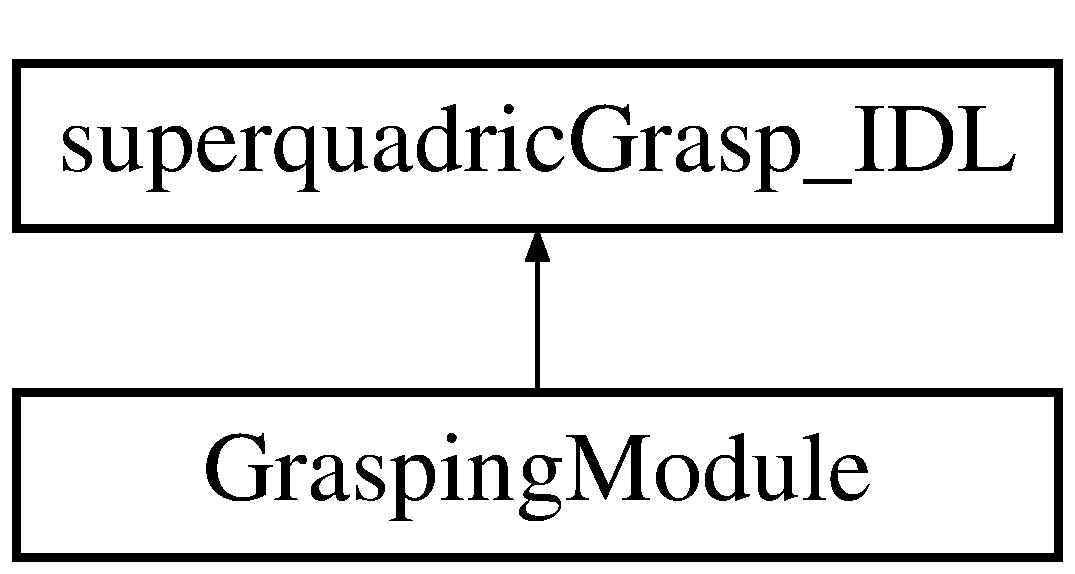
\includegraphics[height=2.000000cm]{classsuperquadricGrasp__IDL}
\end{center}
\end{figure}
\subsection*{Public Member Functions}
\begin{DoxyCompactItemize}
\item 
virtual bool \hyperlink{classsuperquadricGrasp__IDL_a6d1e4533ad8b34510ba9792f7cd72113}{clear\+\_\+poses} ()
\begin{DoxyCompactList}\small\item\em Remove computed poses. \end{DoxyCompactList}\item 
virtual bool \hyperlink{classsuperquadricGrasp__IDL_a6215b75f080a5837599b25826c142921}{set\+\_\+hand} (const std\+::string \&hand)
\begin{DoxyCompactList}\small\item\em Choose the hand to use to grasp the object. \end{DoxyCompactList}\item 
virtual std\+::string \hyperlink{classsuperquadricGrasp__IDL_ad1e5b402e403bc6765d7bf7e8fff0e91}{get\+\_\+hand} ()
\begin{DoxyCompactList}\small\item\em Get the chosen hand. \end{DoxyCompactList}\item 
virtual bool \hyperlink{classsuperquadricGrasp__IDL_ac01ec2012d2b12098a86f7f053068464}{set\+\_\+save\+\_\+poses} (const std\+::string \&entry)
\begin{DoxyCompactList}\small\item\em Set if to save or not the computed poses and trajectory. \end{DoxyCompactList}\item 
virtual std\+::string \hyperlink{classsuperquadricGrasp__IDL_aab45b0423b4e2d440b8a1256c1d6bdfc}{get\+\_\+save\+\_\+poses} ()
\begin{DoxyCompactList}\small\item\em Get if the saving process is on or off. \end{DoxyCompactList}\item 
virtual bool \hyperlink{classsuperquadricGrasp__IDL_a5320ef56cf3da687e7cf678b2a9397f5}{set\+\_\+options} (const yarp\+::os\+::\+Property \&options, const std\+::string \&field)
\begin{DoxyCompactList}\small\item\em Set the parameters of the module. \end{DoxyCompactList}\item 
virtual yarp\+::os\+::\+Property \hyperlink{classsuperquadricGrasp__IDL_a4799064cf16a52762787c0b245318d54}{get\+\_\+options} (const std\+::string \&field)
\begin{DoxyCompactList}\small\item\em Get the parameters of the module. \end{DoxyCompactList}\item 
virtual yarp\+::os\+::\+Property \hyperlink{classsuperquadricGrasp__IDL_a595e98ed2a8fca7ac707b71f97d626d1}{get\+\_\+grasping\+\_\+pose} (const yarp\+::os\+::\+Property \&estimated\+\_\+superq, const std\+::string \&hand)
\begin{DoxyCompactList}\small\item\em Return the estimated grasping poses given an estimated superquadric. \end{DoxyCompactList}\item 
virtual bool \hyperlink{classsuperquadricGrasp__IDL_a91d43de48ad97e35205010c7510e503c}{set\+\_\+visualization} (const std\+::string \&e)
\begin{DoxyCompactList}\small\item\em Set if the visualization has to be enabled. \end{DoxyCompactList}\item 
virtual std\+::string \hyperlink{classsuperquadricGrasp__IDL_ad108d67db8f389b630fa2b0caed87ca5}{get\+\_\+visualization} ()
\begin{DoxyCompactList}\small\item\em Get if visualization is enabled. \end{DoxyCompactList}\item 
virtual bool \hyperlink{classsuperquadricGrasp__IDL_aa996e476a845b484542c7a596cc1f02a}{move} (const std\+::string \&e)
\begin{DoxyCompactList}\small\item\em Move the right or the left arm (according to the string e). \end{DoxyCompactList}\item 
virtual bool {\bfseries look\+\_\+center} ()\label{classsuperquadricGrasp__IDL_a2f9efa6904f4e7240456a4968f3f6c07}

\item 
virtual bool {\bfseries look\+\_\+obj} ()\label{classsuperquadricGrasp__IDL_ad583966fde84372bad2b65214dcbe2bc}

\item 
virtual bool \hyperlink{classsuperquadricGrasp__IDL_a67b63b85635a02ab15f9447ad2b1b0dd}{go\+\_\+home} (const std\+::string \&e)
\begin{DoxyCompactList}\small\item\em Move the right or the left arm back to home position (according to the string e). \end{DoxyCompactList}\item 
virtual bool \hyperlink{classsuperquadricGrasp__IDL_abafbd89252eed10caf876ff1965491d0}{go\+\_\+to\+\_\+basket} (const std\+::string \&e)
\begin{DoxyCompactList}\small\item\em Move the right or the left arm to the basket (according to the string e). \end{DoxyCompactList}\item 
virtual std\+::string \hyperlink{classsuperquadricGrasp__IDL_afca9a01bade8e22262e5e70a96d671ae}{get\+\_\+best\+\_\+hand} ()
\begin{DoxyCompactList}\small\item\em Get the name of the best hand for grasping the object. \end{DoxyCompactList}\item 
virtual bool \hyperlink{classsuperquadricGrasp__IDL_afd0cc265ba84c844aee5654f1a713fbd}{check\+\_\+motion} ()
\begin{DoxyCompactList}\small\item\em Check if the motion has been completed. \end{DoxyCompactList}\item 
virtual bool \hyperlink{classsuperquadricGrasp__IDL_a9e11fd04a40c86987500c42f898508ea}{check\+\_\+home} ()
\begin{DoxyCompactList}\small\item\em Check if the motion back to home has been completed. \end{DoxyCompactList}\item 
virtual bool \hyperlink{classsuperquadricGrasp__IDL_ac40ef7c0dd4f0e3600db9aea5cc5c298}{calibrate} ()
\begin{DoxyCompactList}\small\item\em Calibrate plane height via superquadric computation. \end{DoxyCompactList}\item 
virtual bool {\bfseries read} (yarp\+::os\+::\+Connection\+Reader \&connection) Y\+A\+R\+P\+\_\+\+O\+V\+E\+R\+R\+I\+DE\label{classsuperquadricGrasp__IDL_a710271cfee0c9b1a31707d84f194b69b}

\item 
virtual std\+::vector$<$ std\+::string $>$ {\bfseries help} (const std\+::string \&function\+Name=\char`\"{}-\/-\/all\char`\"{})\label{classsuperquadricGrasp__IDL_a226f766d3a3a0ba87e7c1fa0aceb2cb8}

\end{DoxyCompactItemize}


\subsection{Detailed Description}
\hyperlink{classsuperquadricGrasp__IDL}{superquadric\+Grasp\+\_\+\+I\+DL} I\+DL Interface to superquadric-\/grasp services. 

Definition at line 18 of file superquadric\+Grasp\+\_\+\+I\+D\+L.\+h.



\subsection{Member Function Documentation}
\index{superquadric\+Grasp\+\_\+\+I\+DL@{superquadric\+Grasp\+\_\+\+I\+DL}!calibrate@{calibrate}}
\index{calibrate@{calibrate}!superquadric\+Grasp\+\_\+\+I\+DL@{superquadric\+Grasp\+\_\+\+I\+DL}}
\subsubsection[{\texorpdfstring{calibrate()}{calibrate()}}]{\setlength{\rightskip}{0pt plus 5cm}virtual bool superquadric\+Grasp\+\_\+\+I\+D\+L\+::calibrate (
\begin{DoxyParamCaption}
{}
\end{DoxyParamCaption}
)\hspace{0.3cm}{\ttfamily [virtual]}}\label{classsuperquadricGrasp__IDL_ac40ef7c0dd4f0e3600db9aea5cc5c298}


Calibrate plane height via superquadric computation. 

\begin{DoxyReturn}{Returns}
true/false on success/failure. 
\end{DoxyReturn}
\index{superquadric\+Grasp\+\_\+\+I\+DL@{superquadric\+Grasp\+\_\+\+I\+DL}!check\+\_\+home@{check\+\_\+home}}
\index{check\+\_\+home@{check\+\_\+home}!superquadric\+Grasp\+\_\+\+I\+DL@{superquadric\+Grasp\+\_\+\+I\+DL}}
\subsubsection[{\texorpdfstring{check\+\_\+home()}{check_home()}}]{\setlength{\rightskip}{0pt plus 5cm}virtual bool superquadric\+Grasp\+\_\+\+I\+D\+L\+::check\+\_\+home (
\begin{DoxyParamCaption}
{}
\end{DoxyParamCaption}
)\hspace{0.3cm}{\ttfamily [virtual]}}\label{classsuperquadricGrasp__IDL_a9e11fd04a40c86987500c42f898508ea}


Check if the motion back to home has been completed. 

\begin{DoxyReturn}{Returns}
true/false on success/failure 
\end{DoxyReturn}


Reimplemented in \hyperlink{classGraspingModule_a650c026153e3a7b0044f508cf9d4bf00}{Grasping\+Module}.

\index{superquadric\+Grasp\+\_\+\+I\+DL@{superquadric\+Grasp\+\_\+\+I\+DL}!check\+\_\+motion@{check\+\_\+motion}}
\index{check\+\_\+motion@{check\+\_\+motion}!superquadric\+Grasp\+\_\+\+I\+DL@{superquadric\+Grasp\+\_\+\+I\+DL}}
\subsubsection[{\texorpdfstring{check\+\_\+motion()}{check_motion()}}]{\setlength{\rightskip}{0pt plus 5cm}virtual bool superquadric\+Grasp\+\_\+\+I\+D\+L\+::check\+\_\+motion (
\begin{DoxyParamCaption}
{}
\end{DoxyParamCaption}
)\hspace{0.3cm}{\ttfamily [virtual]}}\label{classsuperquadricGrasp__IDL_afd0cc265ba84c844aee5654f1a713fbd}


Check if the motion has been completed. 

\begin{DoxyReturn}{Returns}
true/false on success/failure 
\end{DoxyReturn}


Reimplemented in \hyperlink{classGraspingModule_a91eac72e632f224442f34b907e479fa3}{Grasping\+Module}.

\index{superquadric\+Grasp\+\_\+\+I\+DL@{superquadric\+Grasp\+\_\+\+I\+DL}!clear\+\_\+poses@{clear\+\_\+poses}}
\index{clear\+\_\+poses@{clear\+\_\+poses}!superquadric\+Grasp\+\_\+\+I\+DL@{superquadric\+Grasp\+\_\+\+I\+DL}}
\subsubsection[{\texorpdfstring{clear\+\_\+poses()}{clear_poses()}}]{\setlength{\rightskip}{0pt plus 5cm}virtual bool superquadric\+Grasp\+\_\+\+I\+D\+L\+::clear\+\_\+poses (
\begin{DoxyParamCaption}
{}
\end{DoxyParamCaption}
)\hspace{0.3cm}{\ttfamily [virtual]}}\label{classsuperquadricGrasp__IDL_a6d1e4533ad8b34510ba9792f7cd72113}


Remove computed poses. 

\begin{DoxyReturn}{Returns}
true/false on success/failure. 
\end{DoxyReturn}


Reimplemented in \hyperlink{classGraspingModule_a834e972a2a1b7b92bf8dc1e83319b028}{Grasping\+Module}.

\index{superquadric\+Grasp\+\_\+\+I\+DL@{superquadric\+Grasp\+\_\+\+I\+DL}!get\+\_\+best\+\_\+hand@{get\+\_\+best\+\_\+hand}}
\index{get\+\_\+best\+\_\+hand@{get\+\_\+best\+\_\+hand}!superquadric\+Grasp\+\_\+\+I\+DL@{superquadric\+Grasp\+\_\+\+I\+DL}}
\subsubsection[{\texorpdfstring{get\+\_\+best\+\_\+hand()}{get_best_hand()}}]{\setlength{\rightskip}{0pt plus 5cm}virtual std\+::string superquadric\+Grasp\+\_\+\+I\+D\+L\+::get\+\_\+best\+\_\+hand (
\begin{DoxyParamCaption}
{}
\end{DoxyParamCaption}
)\hspace{0.3cm}{\ttfamily [virtual]}}\label{classsuperquadricGrasp__IDL_afca9a01bade8e22262e5e70a96d671ae}


Get the name of the best hand for grasping the object. 

\begin{DoxyReturn}{Returns}
right or left 
\end{DoxyReturn}


Reimplemented in \hyperlink{classGraspingModule_a5103f8bd6671a11a9bd1c7e29d290009}{Grasping\+Module}.

\index{superquadric\+Grasp\+\_\+\+I\+DL@{superquadric\+Grasp\+\_\+\+I\+DL}!get\+\_\+grasping\+\_\+pose@{get\+\_\+grasping\+\_\+pose}}
\index{get\+\_\+grasping\+\_\+pose@{get\+\_\+grasping\+\_\+pose}!superquadric\+Grasp\+\_\+\+I\+DL@{superquadric\+Grasp\+\_\+\+I\+DL}}
\subsubsection[{\texorpdfstring{get\+\_\+grasping\+\_\+pose(const yarp\+::os\+::\+Property \&estimated\+\_\+superq, const std\+::string \&hand)}{get_grasping_pose(const yarp::os::Property &estimated_superq, const std::string &hand)}}]{\setlength{\rightskip}{0pt plus 5cm}virtual yarp\+::os\+::\+Property superquadric\+Grasp\+\_\+\+I\+D\+L\+::get\+\_\+grasping\+\_\+pose (
\begin{DoxyParamCaption}
\item[{const yarp\+::os\+::\+Property \&}]{estimated\+\_\+superq, }
\item[{const std\+::string \&}]{hand}
\end{DoxyParamCaption}
)\hspace{0.3cm}{\ttfamily [virtual]}}\label{classsuperquadricGrasp__IDL_a595e98ed2a8fca7ac707b71f97d626d1}


Return the estimated grasping poses given an estimated superquadric. 


\begin{DoxyParams}{Parameters}
{\em estimated\+\_\+superq} & is a Property containing the superquadric. \\
\hline
{\em hand} & is the hand for which we want to solve the grasping problem (right, left or both). \\
\hline
\end{DoxyParams}
\begin{DoxyReturn}{Returns}
a property containing the solution. Note\+: the estimated superquadric must be provide in the following format\+: (dimensions (x0 x1 x2)) (exponents (x3 x4)) (center (x5 x6 x7)) (orientation (x8 x9 x10 x11)) where x0, x1,x2 are the semi axes of the superquadric, x3, x4 are the responsible for the shape, x5 x6 x7 are the coordinates of the superquadric center and x8 x9 x10 x11 are the axis-\/angle representation of the superquadric orientation. The solution is given in the form\+: (pose\+\_\+right (h0 h1 h2 h3 h4 h5 h6)) (trajectory\+\_\+right (t0 t1 t2 t3 t4 t5) ... ) for the right hand, and the same for the left hand (according to the value of the string hand are input parameter. The quantity \char`\"{}pose\+\_\+right\char`\"{} is the pose computed for the robot hand (x0,x1,x2, are the 3D coordinates of the end-\/effector and x3,x4,x5 are the Euler angles representing the end-\/effector orientation) The quantity \char`\"{}trajectory\+\_\+right\char`\"{} includes all the waypoint of the computed trajectory, in the form center of the end-\/effector (t0,t1,t2)+ orientation (Euler angles, t3,t4,t5). 
\end{DoxyReturn}


Reimplemented in \hyperlink{classGraspingModule_af1e057f767ab83be185cf486d3f5c46b}{Grasping\+Module}.

\index{superquadric\+Grasp\+\_\+\+I\+DL@{superquadric\+Grasp\+\_\+\+I\+DL}!get\+\_\+hand@{get\+\_\+hand}}
\index{get\+\_\+hand@{get\+\_\+hand}!superquadric\+Grasp\+\_\+\+I\+DL@{superquadric\+Grasp\+\_\+\+I\+DL}}
\subsubsection[{\texorpdfstring{get\+\_\+hand()}{get_hand()}}]{\setlength{\rightskip}{0pt plus 5cm}virtual std\+::string superquadric\+Grasp\+\_\+\+I\+D\+L\+::get\+\_\+hand (
\begin{DoxyParamCaption}
{}
\end{DoxyParamCaption}
)\hspace{0.3cm}{\ttfamily [virtual]}}\label{classsuperquadricGrasp__IDL_ad1e5b402e403bc6765d7bf7e8fff0e91}


Get the chosen hand. 

\begin{DoxyReturn}{Returns}
left or right. 
\end{DoxyReturn}


Reimplemented in \hyperlink{classGraspingModule_a557a87131c7396dd62c02eced7f4a937}{Grasping\+Module}.

\index{superquadric\+Grasp\+\_\+\+I\+DL@{superquadric\+Grasp\+\_\+\+I\+DL}!get\+\_\+options@{get\+\_\+options}}
\index{get\+\_\+options@{get\+\_\+options}!superquadric\+Grasp\+\_\+\+I\+DL@{superquadric\+Grasp\+\_\+\+I\+DL}}
\subsubsection[{\texorpdfstring{get\+\_\+options(const std\+::string \&field)}{get_options(const std::string &field)}}]{\setlength{\rightskip}{0pt plus 5cm}virtual yarp\+::os\+::\+Property superquadric\+Grasp\+\_\+\+I\+D\+L\+::get\+\_\+options (
\begin{DoxyParamCaption}
\item[{const std\+::string \&}]{field}
\end{DoxyParamCaption}
)\hspace{0.3cm}{\ttfamily [virtual]}}\label{classsuperquadricGrasp__IDL_a4799064cf16a52762787c0b245318d54}


Get the parameters of the module. 

The user must pay attention in changing them. 
\begin{DoxyParams}{Parameters}
{\em field} & can be \char`\"{}pose\char`\"{}, \char`\"{}trajectory\char`\"{}, \char`\"{}optimization\char`\"{}, \char`\"{}statistics\char`\"{}, \char`\"{}visualization\char`\"{} or \char`\"{}execution\char`\"{}. depending on which parameters we are interested in. \\
\hline
\end{DoxyParams}
\begin{DoxyReturn}{Returns}
the Property including all the parameter values. 
\end{DoxyReturn}


Reimplemented in \hyperlink{classGraspingModule_a375475691c644d8aa882db8d65ceda50}{Grasping\+Module}.

\index{superquadric\+Grasp\+\_\+\+I\+DL@{superquadric\+Grasp\+\_\+\+I\+DL}!get\+\_\+save\+\_\+poses@{get\+\_\+save\+\_\+poses}}
\index{get\+\_\+save\+\_\+poses@{get\+\_\+save\+\_\+poses}!superquadric\+Grasp\+\_\+\+I\+DL@{superquadric\+Grasp\+\_\+\+I\+DL}}
\subsubsection[{\texorpdfstring{get\+\_\+save\+\_\+poses()}{get_save_poses()}}]{\setlength{\rightskip}{0pt plus 5cm}virtual std\+::string superquadric\+Grasp\+\_\+\+I\+D\+L\+::get\+\_\+save\+\_\+poses (
\begin{DoxyParamCaption}
{}
\end{DoxyParamCaption}
)\hspace{0.3cm}{\ttfamily [virtual]}}\label{classsuperquadricGrasp__IDL_aab45b0423b4e2d440b8a1256c1d6bdfc}


Get if the saving process is on or off. 

\begin{DoxyReturn}{Returns}
\char`\"{}on\char`\"{} or \char`\"{}off\char`\"{}. 
\end{DoxyReturn}


Reimplemented in \hyperlink{classGraspingModule_a949e4297bdf26f564669ffc91068c4f3}{Grasping\+Module}.

\index{superquadric\+Grasp\+\_\+\+I\+DL@{superquadric\+Grasp\+\_\+\+I\+DL}!get\+\_\+visualization@{get\+\_\+visualization}}
\index{get\+\_\+visualization@{get\+\_\+visualization}!superquadric\+Grasp\+\_\+\+I\+DL@{superquadric\+Grasp\+\_\+\+I\+DL}}
\subsubsection[{\texorpdfstring{get\+\_\+visualization()}{get_visualization()}}]{\setlength{\rightskip}{0pt plus 5cm}virtual std\+::string superquadric\+Grasp\+\_\+\+I\+D\+L\+::get\+\_\+visualization (
\begin{DoxyParamCaption}
{}
\end{DoxyParamCaption}
)\hspace{0.3cm}{\ttfamily [virtual]}}\label{classsuperquadricGrasp__IDL_ad108d67db8f389b630fa2b0caed87ca5}


Get if visualization is enabled. 

\begin{DoxyReturn}{Returns}
\char`\"{}on\char`\"{} or \char`\"{}off\char`\"{}. 
\end{DoxyReturn}


Reimplemented in \hyperlink{classGraspingModule_aabedec650875263d27ecf20fa9dd8b39}{Grasping\+Module}.

\index{superquadric\+Grasp\+\_\+\+I\+DL@{superquadric\+Grasp\+\_\+\+I\+DL}!go\+\_\+home@{go\+\_\+home}}
\index{go\+\_\+home@{go\+\_\+home}!superquadric\+Grasp\+\_\+\+I\+DL@{superquadric\+Grasp\+\_\+\+I\+DL}}
\subsubsection[{\texorpdfstring{go\+\_\+home(const std\+::string \&e)}{go_home(const std::string &e)}}]{\setlength{\rightskip}{0pt plus 5cm}virtual bool superquadric\+Grasp\+\_\+\+I\+D\+L\+::go\+\_\+home (
\begin{DoxyParamCaption}
\item[{const std\+::string \&}]{e}
\end{DoxyParamCaption}
)\hspace{0.3cm}{\ttfamily [virtual]}}\label{classsuperquadricGrasp__IDL_a67b63b85635a02ab15f9447ad2b1b0dd}


Move the right or the left arm back to home position (according to the string e). 

\begin{DoxyReturn}{Returns}
\char`\"{}on\char`\"{} or \char`\"{}off\char`\"{} if e is right or left. 
\end{DoxyReturn}


Reimplemented in \hyperlink{classGraspingModule_a1455fc4c6a1ae5690fa691cc324fec4e}{Grasping\+Module}.

\index{superquadric\+Grasp\+\_\+\+I\+DL@{superquadric\+Grasp\+\_\+\+I\+DL}!go\+\_\+to\+\_\+basket@{go\+\_\+to\+\_\+basket}}
\index{go\+\_\+to\+\_\+basket@{go\+\_\+to\+\_\+basket}!superquadric\+Grasp\+\_\+\+I\+DL@{superquadric\+Grasp\+\_\+\+I\+DL}}
\subsubsection[{\texorpdfstring{go\+\_\+to\+\_\+basket(const std\+::string \&e)}{go_to_basket(const std::string &e)}}]{\setlength{\rightskip}{0pt plus 5cm}virtual bool superquadric\+Grasp\+\_\+\+I\+D\+L\+::go\+\_\+to\+\_\+basket (
\begin{DoxyParamCaption}
\item[{const std\+::string \&}]{e}
\end{DoxyParamCaption}
)\hspace{0.3cm}{\ttfamily [virtual]}}\label{classsuperquadricGrasp__IDL_abafbd89252eed10caf876ff1965491d0}


Move the right or the left arm to the basket (according to the string e). 

\begin{DoxyReturn}{Returns}
\char`\"{}on\char`\"{} or \char`\"{}off\char`\"{} if e is right or left. 
\end{DoxyReturn}


Reimplemented in \hyperlink{classGraspingModule_a75482819f7f289b3f456571628952122}{Grasping\+Module}.

\index{superquadric\+Grasp\+\_\+\+I\+DL@{superquadric\+Grasp\+\_\+\+I\+DL}!move@{move}}
\index{move@{move}!superquadric\+Grasp\+\_\+\+I\+DL@{superquadric\+Grasp\+\_\+\+I\+DL}}
\subsubsection[{\texorpdfstring{move(const std\+::string \&e)}{move(const std::string &e)}}]{\setlength{\rightskip}{0pt plus 5cm}virtual bool superquadric\+Grasp\+\_\+\+I\+D\+L\+::move (
\begin{DoxyParamCaption}
\item[{const std\+::string \&}]{e}
\end{DoxyParamCaption}
)\hspace{0.3cm}{\ttfamily [virtual]}}\label{classsuperquadricGrasp__IDL_aa996e476a845b484542c7a596cc1f02a}


Move the right or the left arm (according to the string e). 

\begin{DoxyReturn}{Returns}
\char`\"{}on\char`\"{} or \char`\"{}off\char`\"{} if e is right or left. 
\end{DoxyReturn}


Reimplemented in \hyperlink{classGraspingModule_a08bd9cdbb1d16da8616c9769510e2bf1}{Grasping\+Module}.

\index{superquadric\+Grasp\+\_\+\+I\+DL@{superquadric\+Grasp\+\_\+\+I\+DL}!set\+\_\+hand@{set\+\_\+hand}}
\index{set\+\_\+hand@{set\+\_\+hand}!superquadric\+Grasp\+\_\+\+I\+DL@{superquadric\+Grasp\+\_\+\+I\+DL}}
\subsubsection[{\texorpdfstring{set\+\_\+hand(const std\+::string \&hand)}{set_hand(const std::string &hand)}}]{\setlength{\rightskip}{0pt plus 5cm}virtual bool superquadric\+Grasp\+\_\+\+I\+D\+L\+::set\+\_\+hand (
\begin{DoxyParamCaption}
\item[{const std\+::string \&}]{hand}
\end{DoxyParamCaption}
)\hspace{0.3cm}{\ttfamily [virtual]}}\label{classsuperquadricGrasp__IDL_a6215b75f080a5837599b25826c142921}


Choose the hand to use to grasp the object. 


\begin{DoxyParams}{Parameters}
{\em hand} & name (left or right). \\
\hline
\end{DoxyParams}
\begin{DoxyReturn}{Returns}
true/false on success/failure. 
\end{DoxyReturn}


Reimplemented in \hyperlink{classGraspingModule_a9d34cb0521f86dd16648255e640eec90}{Grasping\+Module}.

\index{superquadric\+Grasp\+\_\+\+I\+DL@{superquadric\+Grasp\+\_\+\+I\+DL}!set\+\_\+options@{set\+\_\+options}}
\index{set\+\_\+options@{set\+\_\+options}!superquadric\+Grasp\+\_\+\+I\+DL@{superquadric\+Grasp\+\_\+\+I\+DL}}
\subsubsection[{\texorpdfstring{set\+\_\+options(const yarp\+::os\+::\+Property \&options, const std\+::string \&field)}{set_options(const yarp::os::Property &options, const std::string &field)}}]{\setlength{\rightskip}{0pt plus 5cm}virtual bool superquadric\+Grasp\+\_\+\+I\+D\+L\+::set\+\_\+options (
\begin{DoxyParamCaption}
\item[{const yarp\+::os\+::\+Property \&}]{options, }
\item[{const std\+::string \&}]{field}
\end{DoxyParamCaption}
)\hspace{0.3cm}{\ttfamily [virtual]}}\label{classsuperquadricGrasp__IDL_a5320ef56cf3da687e7cf678b2a9397f5}


Set the parameters of the module. 

The user must pay attention in changing them. 
\begin{DoxyParams}{Parameters}
{\em options} & is a Property containing the parameters the user want to change. \\
\hline
{\em field} & is a string specifying which can of parameter we are going to change. Field can be\+: \char`\"{}pose\char`\"{}, \char`\"{}trajectory\char`\"{}, \char`\"{}optimization\char`\"{}, \char`\"{}visualization\char`\"{} or \char`\"{}execution\char`\"{}. You can set the parameters typing, for instance\+: command\+: set\+\_\+options ((n\+\_\+pointshand $<$points-\/value$>$) (hand\+\_\+displacement\+\_\+x $<$displacement-\/value$>$)) pose. \\
\hline
\end{DoxyParams}
\begin{DoxyReturn}{Returns}
true/false on success/failure. 
\end{DoxyReturn}


Reimplemented in \hyperlink{classGraspingModule_a849c459ef9700c93b45ef6cff394f675}{Grasping\+Module}.

\index{superquadric\+Grasp\+\_\+\+I\+DL@{superquadric\+Grasp\+\_\+\+I\+DL}!set\+\_\+save\+\_\+poses@{set\+\_\+save\+\_\+poses}}
\index{set\+\_\+save\+\_\+poses@{set\+\_\+save\+\_\+poses}!superquadric\+Grasp\+\_\+\+I\+DL@{superquadric\+Grasp\+\_\+\+I\+DL}}
\subsubsection[{\texorpdfstring{set\+\_\+save\+\_\+poses(const std\+::string \&entry)}{set_save_poses(const std::string &entry)}}]{\setlength{\rightskip}{0pt plus 5cm}virtual bool superquadric\+Grasp\+\_\+\+I\+D\+L\+::set\+\_\+save\+\_\+poses (
\begin{DoxyParamCaption}
\item[{const std\+::string \&}]{entry}
\end{DoxyParamCaption}
)\hspace{0.3cm}{\ttfamily [virtual]}}\label{classsuperquadricGrasp__IDL_ac01ec2012d2b12098a86f7f053068464}


Set if to save or not the computed poses and trajectory. 


\begin{DoxyParams}{Parameters}
{\em entry} & can be \char`\"{}on\char`\"{} or \char`\"{}off\char`\"{}. \\
\hline
\end{DoxyParams}
\begin{DoxyReturn}{Returns}
true/false on success/failure. 
\end{DoxyReturn}


Reimplemented in \hyperlink{classGraspingModule_a618785dec349358760a05e6e4b097866}{Grasping\+Module}.

\index{superquadric\+Grasp\+\_\+\+I\+DL@{superquadric\+Grasp\+\_\+\+I\+DL}!set\+\_\+visualization@{set\+\_\+visualization}}
\index{set\+\_\+visualization@{set\+\_\+visualization}!superquadric\+Grasp\+\_\+\+I\+DL@{superquadric\+Grasp\+\_\+\+I\+DL}}
\subsubsection[{\texorpdfstring{set\+\_\+visualization(const std\+::string \&e)}{set_visualization(const std::string &e)}}]{\setlength{\rightskip}{0pt plus 5cm}virtual bool superquadric\+Grasp\+\_\+\+I\+D\+L\+::set\+\_\+visualization (
\begin{DoxyParamCaption}
\item[{const std\+::string \&}]{e}
\end{DoxyParamCaption}
)\hspace{0.3cm}{\ttfamily [virtual]}}\label{classsuperquadricGrasp__IDL_a91d43de48ad97e35205010c7510e503c}


Set if the visualization has to be enabled. 

\begin{DoxyReturn}{Returns}
true/false on success/failure. 
\end{DoxyReturn}


Reimplemented in \hyperlink{classGraspingModule_a801de4b63aba360a4b85e322c5947a4a}{Grasping\+Module}.



The documentation for this class was generated from the following file\+:\begin{DoxyCompactItemize}
\item 
/home/gvezzani/\+Desktop/\+Ph\+D/\+Anno\+\_\+1/super\+Quadratiche/superquadric-\/grasping/idl\+\_\+dox/superquadric\+Grasp\+\_\+\+I\+D\+L.\+h\end{DoxyCompactItemize}

%--- End generated contents ---

% Index
\backmatter
\newpage
\phantomsection
\clearemptydoublepage
\addcontentsline{toc}{chapter}{Index}
\printindex

\end{document}
